\documentclass[a4paper,11pt]{report}

\usepackage{array}
\usepackage{makeidx}
\usepackage{fullpage}
\usepackage{graphicx}
\usepackage{appendix}
\usepackage[acronym=true]{glossary}

\newcommand{\amu}{\textit{amu}}
\newcommand{\nm}{\textit{nm}}
\newcommand{\nmsquare}{$nm^2$}
\newcommand{\vacfunits}{$nm^2s^{-2}$}
\newcommand{\ps}{\textit{ps}}
\newcommand{\invnm}{$nm^{-1}$}
\newcommand{\ns}{\textit{ns}}
\newcommand{\thz}{\textit{THz}}
\newcommand{\qval}{\textit{q}}
\newcommand{\qvect}{\textit{q}-vector}
\newcommand{\qvects}{\textit{q}-vectors}
\newcommand{\qshell}{\textit{q}-shell}
\newcommand{\qshells}{\textit{q}-shells}
\newcommand{\NMOLDYN}{\textit{n}MOLDYN}

\setcounter{tocdepth}{3}

\setcounter{secnumdepth}{3}
\renewcommand{\labelitemii}{$\star$}

\makeacronym
\newacronym[AC]{\textit{AC}}{\textbf{A}ngular \textbf{C}orrelation}{}
\newacronym[AR]{\textit{AR}}{\textbf{A}uto-\textbf{R}egressive}{}
\newacronym[ARA]{\textit{ARA}}{\textbf{A}uto-\textbf{R}egressive \textbf{A}nalysis}{}
\newacronym[ADOS]{\textit{ADOS}}{\textbf{A}ngular \textbf{D}ensity \textbf{O}f \textbf{S}tates}{}
\newacronym[AVACF]{\textit{AVACF}}{\textbf{A}ngular \textbf{V}elocity \textbf{A}uto\textbf{C}orrelation \textbf{F}unction}{}
\newacronym[CHARMM]{CHARMM}{\textbf{C}hemistry at \textbf{HAR}vard \textbf{M}acromolecular \textbf{M}echanics}{}
\newacronym[CDL]{CDL}{network \textbf{C}ommon \textbf{D}ata \textbf{L}anguage}{}
\newacronym[CN]{\textit{CN}}{\textbf{C}oordination \textbf{N}umber}{}
\newacronym[COMT]{\textit{COMT}}{\textbf{C}enter \textbf{O}f \textbf{M}ass \textbf{T}rajectory}{}
\newacronym[DCSF]{\textit{DCSF}}{\textbf{D}ynamic \textbf{C}oherent \textbf{S}tructure \textbf{F}actor}{}
\newacronym[DCSFAR]{\textit{DCSFAR}}{\textbf{D}ynamic \textbf{C}oherent \textbf{S}tructure \textbf{F}actor using an \textbf{A}uto-\textbf{R}egressive model}{}
\newacronym[DISF]{\textit{DISF}}{\textbf{D}ynamic \textbf{I}ncoherent \textbf{S}tructure \textbf{F}actor}{}
\newacronym[DISFAR]{\textit{DISFAR}}{\textbf{D}ynamic \textbf{I}ncoherent \textbf{S}tructure \textbf{F}actor using an \textbf{A}uto-\textbf{R}egressive model}{}
\newacronym[DISFG]{\textit{DISFG}}{\textbf{D}ynamic \textbf{I}ncoherent \textbf{S}tructure \textbf{F}actor using an \textbf{G}aussian approximation}{}
\newacronym[DOS]{\textit{DOS}}{\textbf{D}ensity \textbf{O}f \textbf{S}tates}{}
\newacronym[FCA]{FCA}{\textbf{F}ast \textbf{C}orrelation \textbf{A}lgorithm}{}
\newacronym[EISF]{\textit{EISF}}{\textbf{E}lastic \textbf{I}ncoherent \textbf{S}tructure \textbf{F}actor}{}
\newacronym[GMFT]{\textit{GMFT}}{\textbf{G}lobal \textbf{M}otion \textbf{F}iltered \textbf{T}rajectory}{}
\newacronym[GUI]{\textit{GUI}}{\textbf{G}raphical \textbf{U}ser \textbf{I}nterface}{}
\newacronym[MD]{MD}{\textbf{M}olecular \textbf{D}ynamics}{}
\newacronym[MMTK]{MMTK}{\textbf{M}olecular \textbf{M}odelling \textbf{T}ool\textbf{K}it}{}
\newacronym[MSD]{\textit{MSD}}{\textbf{M}ean-\textbf{S}quare \textbf{D}isplacement}{}
\newacronym[NAMD]{NAMD}{\textbf{NA}noscale \textbf{M}olecular \textbf{D}ynamics}{}
\newacronym[NetCDF]{NetCDF}{\textbf{N}etwork \textbf{C}ommon \textbf{D}ata \textbf{F}orm}{}
\newacronym[PBFT]{\textit{PBFT}}{\textbf{P}ass-\textbf{B}and \textbf{F}iltered \textbf{T}rajectory}{}
\newacronym[OP]{\textit{OP}}{\textbf{O}rder \textbf{P}arameter}{}
\newacronym[OPCM]{\textit{OPCM}}{\textbf{O}rder \textbf{P}arameter using \textbf{C}ontact \textbf{M}odel}{}
\newacronym[PDF]{\textit{PDF}}{\textbf{P}air-\textbf{D}istribution \textbf{F}unction}{}
\newacronym[PDB]{\textit{PDB}}{\textbf{P}rotein \textbf{D}ata \textbf{B}ank}{}
\newacronym[QHA]{\textit{QHA}}{\textbf{Q}uasi-\textbf{H}armonic \textbf{A}nalysis}{}
\newacronym[RBT]{\textit{RBT}}{\textbf{R}igid-\textbf{B}ody \textbf{T}rajectory}{}
\newacronym[RCF]{\textit{RCF}}{\textbf{R}eorientational \textbf{C}orrelation \textbf{F}unction}{}
\newacronym[RDF]{\textit{RDF}}{\textbf{R}adial-\textbf{D}istribution \textbf{F}unction}{}
\newacronym[ROG]{\textit{ROG}}{\textbf{R}adius \textbf{O}f \textbf{G}yration}{}
\newacronym[RMSD]{\textit{RMSD}}{\textbf{R}oot \textbf{M}ean-\textbf{S}quare \textbf{D}eviation}{}
\newacronym[SCSF]{\textit{SCSF}}{\textbf{S}tatic \textbf{C}oherent \textbf{S}tructure \textbf{F}actor}{}
\newacronym[SD]{\textit{SD}}{\textbf{S}patial \textbf{D}ensity}{}
\newacronym[SFA]{\textit{SFA}}{\textbf{S}crew\textbf{F}it \textbf{A}nalysis}{}
\newacronym[SSCSF]{\textit{SSCSF}}{\textbf{S}moothed \textbf{S}tatic \textbf{C}oherent \textbf{S}tructure \textbf{F}actor}{}
\newacronym[TCF]{\textit{TCF}}{\textbf{T}otal-\textbf{C}orrelation \textbf{F}unction}{}
\newacronym[UCAR]{\textit{UCAR}}{\textbf{U}niversity \textbf{C}orporation for \textbf{A}tmospheric \textbf{R}esearch}{}
\newacronym[VACF]{\textit{VACF}}{\textbf{V}elocity \textbf{A}uto\textbf{C}orrelation \textbf{F}unction}{}
\newacronym[VASP]{VASP}{\textbf{V}ienna \textbf{A}b-initio \textbf{S}imulation \textbf{P}ackage}{}
\newacronym[VMD]{VMD}{\textbf{V}isual \textbf{M}olecular \textbf{D}ynamics}{}
\newacronym[XST]{XST}{e\textbf{X}tended \textbf{S}ystem \textbf{T}rajectory}{}
\begin{document}

\begin{titlepage}

\begin{center}


\includegraphics[width=0.60\textwidth]{./Figures/logo.eps}

\vspace{2cm}
 
\vspace{0.5cm}
{\Huge \bfseries \NMOLDYN\ User's Guide}\\
\vspace{0.5cm}
{\huge \bfseries Version 3.4}
\vspace{0.5cm}

\vspace{1.5cm}

{\Large Eric Pellegrini$^{a}$, Paolo Calligari$^{b}$, Vania Calandrini$^{c}$}\\
\vspace{0.5cm}
{\Large Konrad Hinsen$^{c,d}$, Gerald R. Kneller$^{c,d,\dag}$}\\

\vspace{1.0cm}
 
{\large \today}\\

\vspace{1.0cm}

{\large \textbf{Description}}\\

\end{center}

\noindent The \NMOLDYN\ User's Guide describes how to use the various features of the \MD\ analysis program 
\NMOLDYN. This guide includes a description of the capabilities of the program, how to use these capabilities, the necessary 
input files and formats, and a comprehensive list of the analysis available in the program and how to set up an run these analysis.

\footnote{$^{a}$Institut Laue-Langevin 6, rue Jules Horowitz BP 156 - 38042 Grenoble Cedex 9, France\\
$^{b}$Ecole Normale Sup\'erieure 24, rue Lhomond - 75231 Paris CEDEX 5, France\\
$^{c}$Centre de Biophysique Moleculaire, CNRS Rue Charles Sadron, 45071 Orleans, Cedex 02, France\\
$^{d}$Synchrotron Soleil - Division Experiences, Saint Aubin - BP 48 91192 Gif sur Yvette Cedex, France\\
$^{\dag}$Corresponding author. Electronic mail:{\tt kneller$@$cnrs-orleans.fr}}

\end{titlepage}

\begin{abstract}
\NMOLDYN\ is a modular program package for the analysis of \MD\ trajectories, especially designed for 
the computation and decomposition of neutron scattering spectra.  

The current release 3.0 of \NMOLDYN\ is an upgrade of the version \NMOLDYN\ 2.0 \cite{Rog}, which extends the functionality of the
original version \NMOLDYN\ 1.0 \cite{Schiller}. It provides an improved user interface (both graphical/interactive 
and batch), and can be used as a tool set for implementing new analysis modules.

\NMOLDYN\ allows one to calculate several dynamics quantities such as the mean-square displacement, the velocity autocorrelation 
function as well as its Fourier Transform (the density of states) and its memory functions, the angular velocity 
autocorrelation function and its Fourier transform, the reorientational correlation function \dots Moreover it
can compute several quantities related to neutron scattering such as the coherent and incoherent intermediate scattering 
functions with their Fourier transforms and their memory functions, the elastic incoherent structure factor, the static 
coherent structure factor or the radial distribution function. Additionally, the \NMOLDYN\ package allows one to construct 
modified trajectories from an input trajectory; rigid-body trajectories, in which the internal motions of the molecules 
(or parts thereof) are eliminated, frequency-filtered trajectories, from which motions outside a specified frequency 
interval are eliminated, global motion filtered trajectory where the global rotation and translation are removed from 
the input trajectory \ldots

All \NMOLDYN\ calculations can be applied to a whole system or to arbitrary subsets. The most common subsets can be selected in 
the graphical interface, less common selections can be specified by Python code via the command-line interface.

As \NMOLDYN\ 2.0, \NMOLDYN\ 3.0 uses \MMTK \cite{Hinsen:2000,MMTK}, an Open Source program library for molecular 
simulation applications, and expects trajectories to be in \MMTK\ format (\NetCDF\ \cite{NetCDF,Davies}). However, many 
trajectory converters are included in the distribution of \NMOLDYN. \NMOLDYN\ 3.0, was written by Eric Pellegrini.
\end{abstract}

\newpage
\tableofcontents
\addcontentsline{toc}{chapter}{Table of Contents}
\newpage
\listoffigures
\addcontentsline{toc}{chapter}{List of Figures}
\newpage
\listoftables
\addcontentsline{toc}{chapter}{List of Tables}
\newpage
\printacronym
\newpage

\chapter{Introduction}
\label{global_introduction}

Although \MD\ simulation techniques are widely used in physics, chemistry and biology, their possibilities 
are often not fully exploited because of the lack of easy-to-use analysis tools. This is especially true for very complex 
systems which force most computational scientists to use standard program packages containing only very limited 
functionality to analyze \MD\ trajectories.

In this NOTE we present the new release 3.0 of the modular program package \NMOLDYN, which replaces the original version 
\NMOLDYN\ 2.0, for the analysis of \MD\ trajectories.

The program \NMOLDYN\ was developed mainly for use in connection with neutron scattering experiment, although many of 
the quantities are also used in other contexts. The combination of neutron scattering experiments and \MD\ 
simulations is a powerful tool to study the structure and dynamics of complex molecular systems. Neutron scattering 
is sensitive to time and space correlations of atomic positions on the \ns\ time scale and the \AA\, length scale 
\cite{Lovesey, Bee}. These are exactly the time and space domains covered by classical \MD\ simulations. 
On the length scale under consideration the neutron-target interaction can be modelled by pseudopotentials with zero range 
which are centered on the atomic nuclei of the targets. The coupling between neutron and target is described by so-called
scattering lengths describing the strength of the neutron-nucleus interaction \cite{Lovesey}.  The differential scattering 
cross section can be expressed in terms of quantum time correlation functions of the spatially Fourier transformed particle 
density. The corresponding \textit{classical} time correlation function can be easily obtained from \MD\ 
simulations.  This enables a direct comparison between simulated and measured neutron scattering intensities for classical 
systems if recoil effects in the scattering process are not dominant \cite{Kneller:1994}. The experimental data can be used 
to test the quality of the \MD\ force field which is the central input for the simulations \cite{Geiger:1989,Geiger:1990,Ahlrichs,Yip:1987}. 
Conversely, the simulated intensities allow a detailed analysis of the dynamical and structural behaviour of the system 
under consideration \cite{Smith:1992,Smith:1993}. The latter is particularly important for complex systems for which 
an interpretation of the measured intensities in terms of simple analytical models is difficult, if not impossible.

The program package \NMOLDYN\ allows neutron scattering intensities to be efficiently calculated from \MD\ simulations. 
The calculation of various space and time correlation functions permits a detailed analysis of the structure and dynamics 
of the system under consideration.  \NMOLDYN\ contains modules for the calculation of dynamics-related, scattering-related and 
structure-related properties. In addition rigid body trajectories of subunits of the system can be extracted from molecular 
dynamics trajectory files. These subunits can be arbitrarily defined, their size can range from a few atoms to a whole 
domain in a macromolecule. From the rigid body trajectories angular correlation functions and reorientational correlation 
functions can be obtained.

The third generation \NMOLDYN\ presented here, offers an interactive graphical user interface for standard 
calculations, highly flexible script-based processing for non-standard applications and a machine-independent 
compact binary file format. These improvements were made possible by the use of
\begin{enumerate}
\item \textbf{python}, a high-level object oriented langage \cite{vanRossum,python};
\item \textbf{NumPy}, a python package needed for scientific computing \cite{NumPy};
\item \textbf{NetCDF}, portable binary file format and its corresponding library \cite{NetCDF,Davies};
\item \textbf{Scientific Python}, an additional scientific computing library \cite{Scientific1,Scientific2};
\item \textbf{MMTK}, a molecular simulation library \cite{Hinsen:2000,MMTK}.
\end{enumerate} 
All of these packages are developped and distributed following the Open Source principles \cite{OpenSource}; anyone can use 
and improve them without being hindered by licensing restricitons.
All the time-consuming algorithms use efficient implementations in C or in Pyrex, a language that allows to 
write code that mixes Python and C data types, and compiles it into a C extension for Python \cite{Pyrex}.

This NOTE is organized as follows: 

Section \ref{global_introduction} gives an overview of \NMOLDYN.\\
Section \ref{installing_nmoldyn} gives the instruction to install \NMOLDYN\ properly in an existing python distribution.\\
Section \ref{input_and_output_files} describes the different \NMOLDYN\ file formats.\\
Section \ref{running_nmoldyn_from_the_graphical_user_interface} describes how to set up and run an analysis in \NMOLDYN\ from the \GUI .\\
Section \ref{running_nmoldyn_from_the_command_line_interface} describes how to set up and run an analysis in \NMOLDYN\ from the command-line interface.
\section{New features in version 3.0}
\label{new_features_in_version_3}

\begin{itemize}
\item{Installers for MacOS X, Win32 and linux}

\item{A new Graphical interface}
A brand new graphical interface is implemented with Tk library \cite{Tk}.

\item{A new plotting engine}
A brand bew plotting engine is implemented using matplotlib python library \cite{matplotlib}. This allows to produce high 
quality plots directly from \NMOLDYN.

\item{Trajectory converters}
Some trajectory converters are implemented and made directly accessible from \NMOLDYN\ \GUI . 
Those converters allows the conversion of trajectory coming from Amber9 \cite{Amber}, \CHARMM\ \cite{CHARMM}, DL\_POLY \cite{DL_POLY}, 
MaterialsStudio \cite{MaterialsStudio}, \NAMD\ \cite{NAMD}, \VASP\ \cite{VASP} and X-PLOR \cite{X-PLOR} to \NMOLDYN\ \MMTK\ trajectory input formats.

\item{Converter from NetCDF to ASCII}
A converter from \NetCDF\ to ASCII that wraps ncdump \cite{ncdump} program is implemented.

\item{Converter from ASCII to NetCDF}
A converter from ASCII to \NetCDF\ that wraps ncgen \cite{ncgen} program is implemented.

\item{Pair Distribution Function}
The \PDF\ analysis is implemented using Pyrex code for a faster analysis.

\item{Coordination number}
The \CN\ analysis is implemented using Pyrex code for a faster analysis.

\item{Spatial Density}
The \SD\ analysis is implemented using Pyrex code for a faster analysis.

\item{Radius Of Gyration}
The \ROG\ analysis is implemented.

\item{Root Mean Square Displacement}
The \RMSD\ analysis is implemented.

\item{Center Of Mass Trajectory}
The \COMT\ analysis is implemented. It determines the trajectory of the center of mass of one or several group of atoms.

\item{Global Motion Filter}
The \GMFT\ analysis is implemented. It removes the global translation and rotation degrees of freedom from a trajectory.

\item{Quasi Harmonic Analysis}
The \QHA\ analysis is implemented. It allows for the decomposition of a system into its different modes of vibration.

\item{Static Coherent Structure Factor}
The \SCSF\ analysis is implemented. It allows for the direct computation of the static coherent structure factor.

\item{Smoothed Static Coherent Structure Factor}
The \SSCSF\ analysis is implemented. It allows for the direct computation of the static coherent structure factor withtout 
any \qvects random generation. It is implemented using Pyrex code for a faster analysis.

\item{Order parameter}
The \OP\ analysis is implemented.

\item{Order parameter using the contact model}
The \OPCM\ analysis developped by Zhang \textit{et al.} \cite{Bruschweiler} is implemented.

\item{ScrewFit analysis}
The ScrewFit 2D methode developped by Paolo Calligari and Gerald Kneller \cite{Calligari} is implemented.

\item{Partial terms}
The partials term for all scattering-related properties are now available.

\item{A new atom selection engine}
A brand new and much more powerful atom selection engine is implemented. When setting up an anlysis, 
it allows for the selection from the \GUI\ of almost any kind of subset.
\end{itemize}

\section{User feedback}
\label{user_feedback}
If you have problems installing or running \NMOLDYN\ after reading this document, please send a complete description of the problem 
by email to pellegrini@ill.fr. If you discover and fix a problem not described in this manual we would appreciate if you 
would tell us about this as well, so we can alert other users and incorporate the fix into the public distribution.
Your suggestions are welcome at pellegrini@ill.fr.

\chapter{Installing \NMOLDYN}
\label{installing_nmoldyn}
When downloading \NMOLDYN\ 3 from its website \cite{nMOLDYN1,nMOLDYN2}, you will get the full Python source code 
which is covered by the CeCILL License \cite{CeCILL}. The current stable version of \NMOLDYN\ is 3.0.4. One of the major 
goal of the new \NMOLDYN\ version targeted  an easier installation on the most current platforms respectively Win32 and Unix 
(Linux and MacOS). This has been done with the development of plat-form specific installers.

\NMOLDYN\ needs the following modules/libraries in order to work properly:
\begin{enumerate}
\item{Tcl/Tk version $\geq$ 8.0 \cite{TclTk}},
\item{Python version $\geq$ 2.4 \cite{python}},
\item{Numpy version $\geq$ 1.2 \cite{NumPy}},
\item{matplotlib version $\geq$ 0.98 \cite{matplotlib}},
\item{Pyro version $\geq$ 3.9 \cite{Pyro}},
\item{Scientific Python version $\geq$ 2.8 \cite{Scientific1,Scientific2}},
\item{\MMTK\ version $\geq$ 2.6.0  \cite{Hinsen:2000,MMTK}},
\item{pywin32 version $\geq$ 210 (for a win32 installation only) \cite{pywin32}}.
\end{enumerate}

The version number is important (and even compulsory for python) and in case where you would decide to use older 
versions of those packages, we can not guarantee that \NMOLDYN\ will work properly or even work at all.

\section{Unix users}
\label{unix_users}
The tar/zip source files of \NMOLDYN\ can be downloaded from the site:
\\\\ 
{\itshape http://sourcesup.cru.fr/projects/nmoldyn}.
\\\\
The instructions to install \NMOLDYN\ from this file are:
\begin{enumerate}
\item {\ttfamily tar xzf nMOLDYN-3.x.y.tar.gz (or unzip nMOLDYN-3.x.y.zip)}\\
\item {\ttfamily cd nMOLDYN-3.x.y}\\
\item {\ttfamily python setup.py build}\\
\item {\ttfamily python setup.py install}\\
\end{enumerate}
The last command may require administrator privileges.

\section{Windows users}
\label{window_users}
Installing \NMOLDYN\ on Windows is straightforward. The \NMOLDYN\ windows installer can be downloaded from the site:
\\\\
{\itshape http://sourcesup.cru.fr/projects/nmoldyn}.
\\\\
Once downloaded, to launch the \NMOLDYN\ windows installer, just double-click on it. A dialog will open asking for a confirmation about the 
place where to install \NMOLDYN. By default, this should be the path for your Python installation and that value should not 
be changed unless you have several Python installation on your machine (not recommended).

Currently, the only \NMOLDYN\ Windows installer available was build with Python 2.5. If you want to build a version of 
\NMOLDYN\ compatible with python 2.4, the strategy to adopt is a little bit different. This time, you have to
\begin{enumerate}
\item download the archive \textit{nMOLDYN-3.x.y.zip} or \textit{nMOLDYN-3.x.y.tar.gz};
\item uncompress it in the directory \textit{dir} of your choice;
\item open a DOS shell;
\item go directory \textit{dir};
\item enter {\texttt python.exe setup.py bdist\_wininst}, this will create a \textit{dist} directory containing 
the \NMOLDYN\ Windows installer, \textit{nMOLDYN-3.x.y.win32-py2.4.exe};
\item{double-click on the newly created \textit{nMOLDYN-3.x.y.win32-py2.4.exe} file in the \textit{dist} directory. This 
will install \NMOLDYN}
\end{enumerate}
This strategy should also work with Python 2.6.

\chapter{Input and output files}
\label{input_and_output_files}
Almost, if not all, functionnalities provided by \NMOLDYN\ are based on \NetCDF\ input file. However, in 
certain circumstances \NMOLDYN\ can use or produce another type of files. We will start this section by 
explaining in details the \NetCDF\ file format format introducing next the other file formats used by \NMOLDYN.

\section{NetCDF file format}
\label{netcdf_file_format}
\NetCDF\ is a set of software libraries and self-describing, machine-independent data formats 
that support the creation, access, and sharing of array-oriented scientific data. The project homepage is hosted by the 
Unidata program at the \UCAR\ \cite{UCAR}. They are also the chief source of \NetCDF\ -based software, standards 
development, updates \ldots \cite{NetCDF_Softwares}. The format is an open standard.

The data format is self-describing. This means that there is a header which describes the layout of the rest of the 
file, in particular the data arrays, as well as arbitrary file metadata in the form of name/value attributes. The format 
is platform independent, with issues such as endianness being addressed in the software libraries. The data arrays 
are rectangular, not ragged, and stored in a simple and regular fashion that allows efficient subsetting.

\NMOLDYN\ expects trajectories to be in \NetCDF\ format and follow the conventions of \MMTK. Trajectories that have not been produced with 
\MMTK\ or \MMTK-based programs must be converted to \MMTK\ format
before they can be analyzed with \NMOLDYN. This conversion is necessary because no other common trajectory format 
permits efficient access both to conformations at a given time and to one-atom trajectories for all times. In
addition to providing such an access, the \NetCDF\ format has several advantages that make it particularly suitable 
for archiving trajectories: 

\begin{itemize}
\item  compact files (binary storage);
\item  machine-independent format;
\item  fully self-contained, complete information about the system is stored in the trajectory file.
\end{itemize}

The conversion of the trajectories from different formats to the \MMTK\ format can be made directly via the 
\NMOLDYN\ graphical user interface (see Section \ref{trajectory_conversion}).

\section{PDB file format}
\label{pdb_file_format}
The \PDB\ file format is used to store coordinate or velocity data. This is the standard format for 
coordinate data for many bioinformatic programs. A full description of this file format can be obtained from the \PDB\ 
web site \cite{PDB}. You can generate \PDB\ files in \NMOLDYN\ by extracting one or several frames from a \MMTK\ 
trajectory file (see Section \ref{frame_snapshot}). \PDB\ files are also used in \NMOLDYN when performing subset, deuteration or group 
selection from a \NMOLDYN\ selection file (see Sections \ref{subset_selection_from_a_selection_file}, 
\ref{deuteration_selection_from_a_selection_file} and \ref{group_selection_from_a_selection_file}).

\section{\NMOLDYN\ preference file}
\label{nmoldyn_preferences_file}
This file will be used by \NMOLDYN\ to setup the preferences (e.g. documenation style, log file path \ldots ). 
It is based on the \textbf{ConfigParser} module of the Python Standard Library \cite{ConfigParser} and as such it must respect the corresponding format.
Section \ref{preferences} will explain how to build, load or save such a file from \NMOLDYN.

\section{\NMOLDYN\ selection files}
\label{nmoldyn_selection_files}
These files allows to perform some subset selection from a \PDB\ file when running an analysis. Their format will 
be explained in Sections \ref{subset_selection_from_a_selection_file}, 
\ref{deuteration_selection_from_a_selection_file} and \ref{group_selection_from_a_selection_file}.

\section{\NMOLDYN\ autostart files}
\label{nmoldyn_autostart_file}
These files are python scripts that allows to run a given analysis just as a classical python script. 
See Section \ref{nmoldyn_autostart_files} for explanations about the format of these files.

\section{\NMOLDYN\ input files}
\label{nmoldyn_input_files}
These files are python scripts that allows to run a given analysis from the \NMOLDYN\ command-line interface. For those 
familiar with \NMOLDYN\ 2, these files correspond to the input scripts that was generated by \textbf{xMOLDYN} and that 
had to be run with \textbf{pMOLDYN}. See Section \ref{nmoldyn_input_files} for explanations about the format of these files.

\chapter{Using \NMOLDYN from the Graphical User Interface}
\label{running_nmoldyn_from_the_graphical_user_interface}

Through the \NMOLDYN\ graphical user interface, you will usually open a trajectory, then specify the parameters 
for the analysis you wish to perform and finally start the calculation itself. But you can also perform some other 
actions such as plotting the results of an analysis, performing some file conversions \ldots The graphical interface gives 
access to most of the functionalities of \NMOLDYN. 
Moreover, from the graphical user interface it is possible to create an input file for the command-line interface or an 
autostart analysis python script. Both kind of files provide a convenient starting point to set up and run new analysis direclty 
from the command-line interface (see Section \ref{running_nmoldyn_from_the_command_line_interface}).
\\
To run \NMOLDYN\ from the \GUI , type the following command line:
\\
\\
{\ttfamily \textit{python-dir}/bin/nMOLDYNStart.py} on unix
\\\\
or
\\\\
{\ttfamily \textit{python-dir}\textbackslash Scripts\textbackslash nMOLDYNStart.py} on Windows
\\
\\
\textit{python-dir} being the prefix of your python distribution. The command line accepts some arguments that can 
change how \NMOLDYN\ will start. The following arguments are currently supported by \NMOLDYN:
\begin{itemize}
\item{\texttt {-h/--help}}\\
\textbf{Format:} not an editable argument\\
\textbf{Value:} \textit{None}\\
\textbf{Description:} displays the details of the command line arguments. \textbf{Will not start \NMOLDYN\ in \GUI\ mode.}

\item{\texttt {--version}}\\
\textbf{Format:} not an editable argument\\
\textbf{Value:} \textit{None}\\
\textbf{Description:} displays the version of \NMOLDYN . \textbf{Will not start \NMOLDYN\ in \GUI\ mode.}

\item{\texttt {-n/--netcdf=}}\\
\textbf{Format:} string\\
\textbf{Value:} \textit{filename}\\
\textbf{Description:} starts \NMOLDYN\ from the graphical user interface loading directly the \textit{filename} \NetCDF\ file.

\item{\texttt {-i/--input=}}\\
\textbf{Format:} string\\
\textbf{Value:} \textit{filename}\\
\textbf{Description:} runs an analysis with the command-line interface using \textit{filename} \NMOLDYN\ input file (see 
Section \ref{nmoldyn_input_files} for details). \textbf{Will not start \NMOLDYN\ in \GUI\ mode.}

\item{\texttt {-c/--contents=}}\\
\textbf{Format:} string\\
\textbf{Value:} \textit{filename molname selkwd}\\
\textbf{Description:} if \textit{file} provided, displays the contents of the trajectory file \textit{file}. If 
\textit{file} and \textit{molname} provided displays the selection keywords associated to \textit{molname}. If 
\textit{file} and \textit{molname} and \textit{selkwd} provided displays the selection values associated to selection 
keyword \textit{selkwd}. \textbf{Will not start \NMOLDYN\ in \GUI\ mode.}

\item{\texttt {-t/--test=}}\\
\textbf{Format: string} \\
\textbf{Value:} \textit{testname}\\
\textbf{Description:} runs one or several analysis benchmarks  \textbf{Will not start the \GUI .} The format for 
\textit{testname} string is
\\\\
\textit{test1,test2,\ldots }
\\\\
where \textit{test1}, \textit{test2} \ldots are the name of benchmark 1, 2 \ldots 
(see Section \ref{analysis_benchmark} for a comprehensive list of the available benchmarks).

\item{\texttt {--acroread\_path=}}\\
\textbf{Format: string} \\
\textbf{Value:} \textit{filename}\\
\textbf{Description:} sets the path for Acrobat Reader executable to \textit{filename}. It will overide the preferences settings.

\item{\texttt {--vmd\_path=}}\\
\textbf{Format:} string\\
\textbf{Value:} \textit{filename}\\
\textbf{Description:} sets the path for VMD executable to \textit{filename}. It will overide the preferences settings.

\item{\texttt {--documentation\_style=}}\\
\textbf{Format:} string\\
\textbf{Value:} \textit{html} or \textit{pdf}\\
\textbf{Description:} sets the format for the online documentation either to HTML (\textit{html}) either to pdf 
(\textit{pdf}). It will overide the preferences settings.

\item{\texttt {--ncdump\_path=}}\\
\textbf{Format:} string\\
\textbf{Value:} \textit{filename}\\
\textbf{Description:} sets the path for \textbf{ncdump} executable to \textit{filename}. It will overide the preferences 
settings.

\item{\texttt {--ncgen\_path=}}\\
\textbf{Format:} string\\
\textbf{Value:} \textit{filename}\\
\textbf{Description:} sets the path for \textbf{ncgen} executable to \textit{filename}. It will overide the preferences 
settings.

\item{\texttt {--outputfile\_path=}}\\
\textbf{Format:} string\\
\textbf{Value:} \textit{dirname}\\
\textbf{Description:} sets the directory where all the output files will be written to \textit{dirname}. It will overide the 
preferences settings.

\item{\texttt {--trajfile\_path=}}\\
\textbf{Format:} string\\
\textbf{Value:} \textit{dirname}\\
\textbf{Description:} sets the default \MMTK\ trajectory input files directory search path to \textit{dirname}. It will 
overide the preferences settings.

\item{\texttt {--warning\_acroread=}}\\
\textbf{Format:} string\\
\textbf{Value:} \textit{yes} or \textit{no}\\
\textbf{Description:} if set to \textit{yes}, will warn you if acrobat reader is not found on your system. It will 
overide the preferences settings.

\item{\texttt {--warning\_ncdump=}}\\
\textbf{Format:} string\\
\textbf{Value:} \textit{yes} or \textit{no}\\
\textbf{Description:} if set to \textit{yes}, will warn you if \textbf{ncdump} program is not found on your system. It will 
overide the preferences settings.

\item{\texttt {--warning\_ncgen=}}\\
\textbf{Format:} string\\
\textbf{Value:} \textit{yes} or \textit{no}\\
\textbf{Description:} if set to \textit{yes}, will warn you if \textbf{ncgen} program is not found on your system. It will 
overide the preferences settings.

\item{\texttt {--warning\_vmd=}}\\
\textbf{Format:} string\\
\textbf{Value:} \textit{yes} or \textit{no}\\
\textbf{Description:} if set to \textit{yes}, will warn you if \textbf{VMD} program is not found on your system. It will 
overide the preferences settings.

\item{\texttt {--progress\_rate=}}\\
\textbf{Format:} integer in [0,100]\\
\textbf{Value:} \textit{prog\_rate}\\
\textbf{Description:} displays the progress of the analysis every \textit{prog\_rate} percents. It will overide the 
preferences settings.
\end{itemize}

When starting \NMOLDYN\ from the \GUI , the start-up window shown in figure \ref{fig:main_dialog} will pop up. This window contains 
four drop down menu buttons,
\begin{itemize}
\item \textbf{File}
\item \textbf{Analysis}
\item \textbf{View}
\item \textbf{Help}
\end{itemize}  
and a text window.
\newpage
\begin{figure}[h!]
\begin{center}
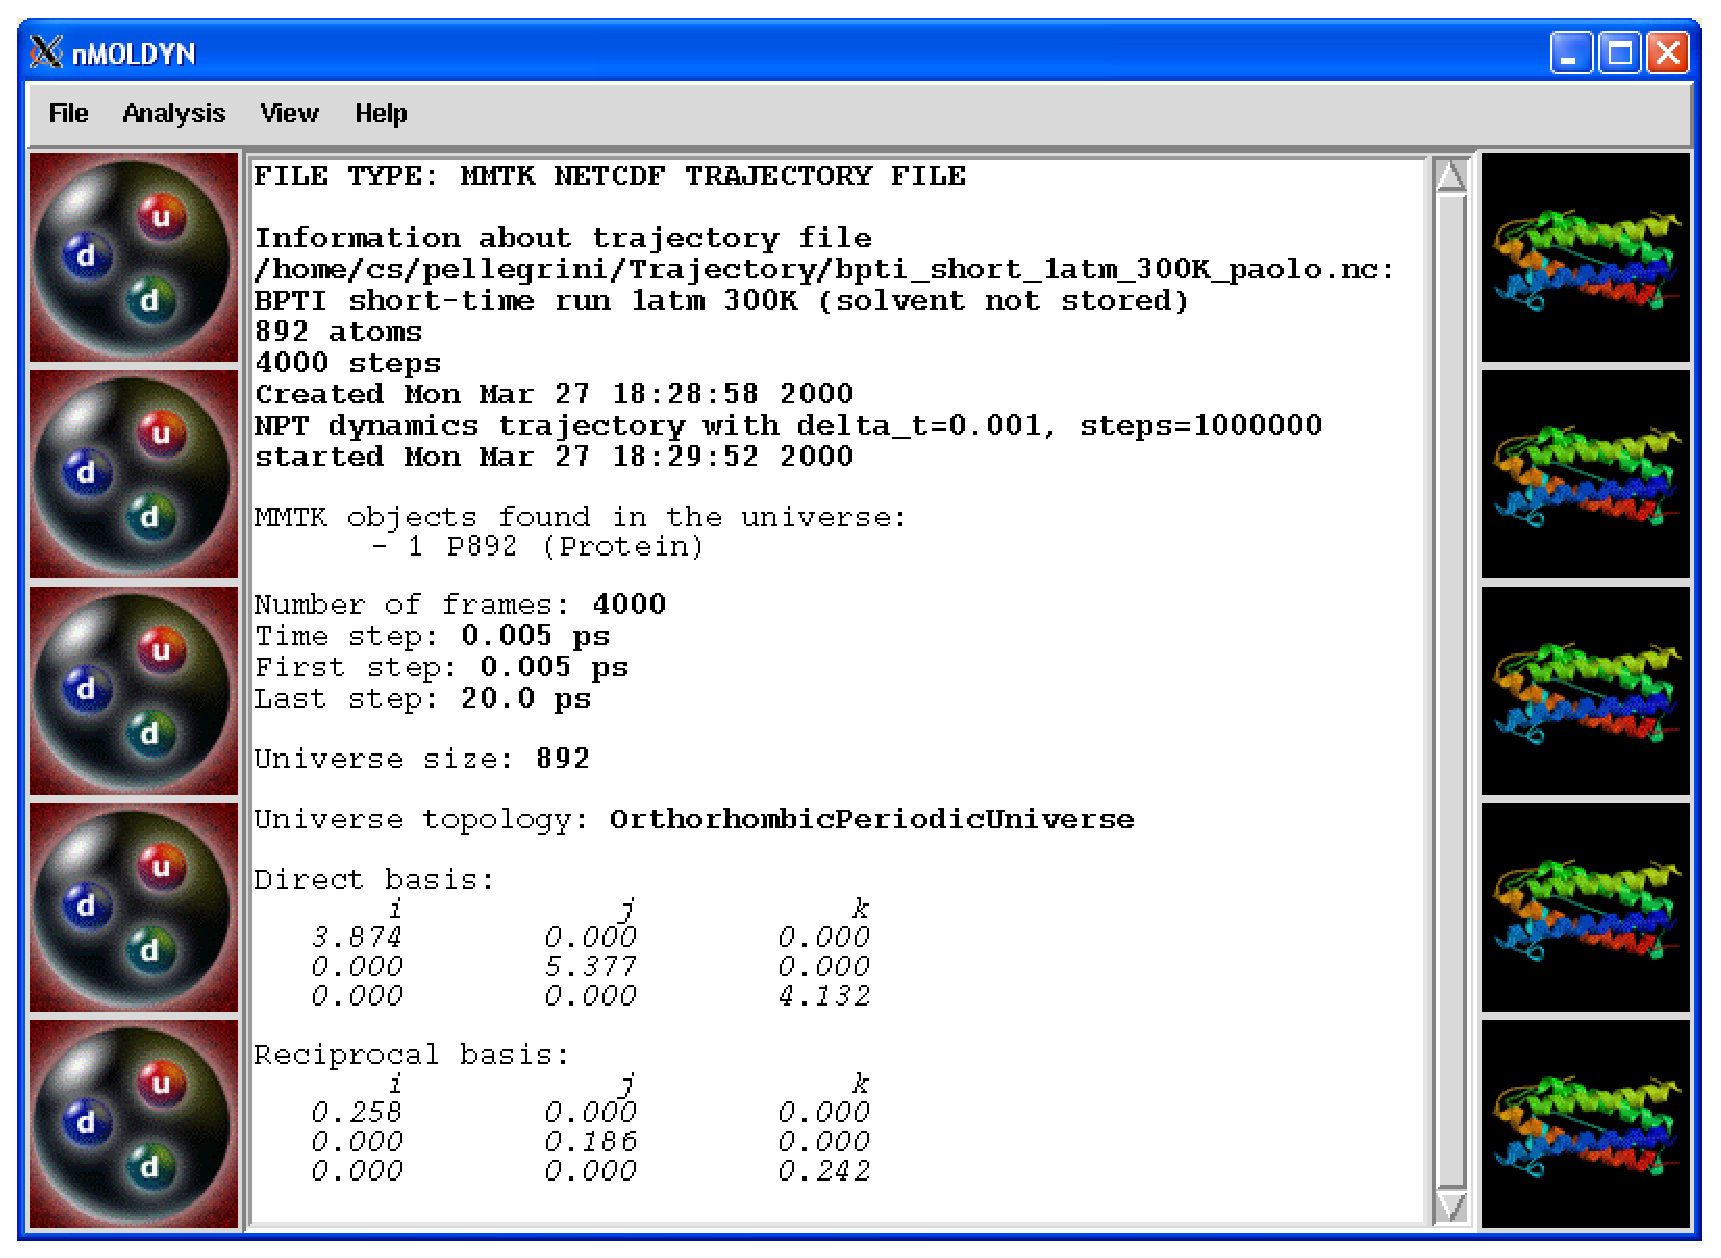
\includegraphics[width=10cm]{Figures/main_dialog.eps}
\end{center}
\caption[The \textit{n}MOLDYN main window]{The \NMOLDYN\ main window.}
\label{fig:main_dialog}
\end{figure}   

Everything concerning IO manipulations are done via the drop down menu button \textbf{File}.
The drop down menu buttons \textbf{Analysis} allows to set up and start the analysis you are interested in.
The \textbf{View} and \textbf{Help} buttons allow one to inspect input/output data and ask for help 
respectively. All of these menus will be described below.Finally,  the text window will display all the information 
concerning the loaded file and the main actions performed on it.

\section{The \textbf{File} menu}
\label{file_menu}
Pressing the \textbf{File} menubutton brings up a menu from which it is possible to choose 
the following options:
\begin{itemize}
\item Load NetCDF file
\item Trajectory conversion
\item Frame snapshot
\item Convert NetCDF to ASCII
\item Convert ASCII to NetCDF
\item Preferences
\item Quit
\end{itemize}
that will be described in the forthcoming sections.

\subsection{Load NetCDF file}
\label{load_netcdf_file}
The \textbf{Load NetCDF file} option allows one to select the \textbf{NetCDF} file
of the trajectory which will be used to perform the analysis. Clicking on it, a file browser like the one showed in figure 
\ref{fig:file_browser} pops up.
\newpage
\begin{figure}[h!]
\begin{center}
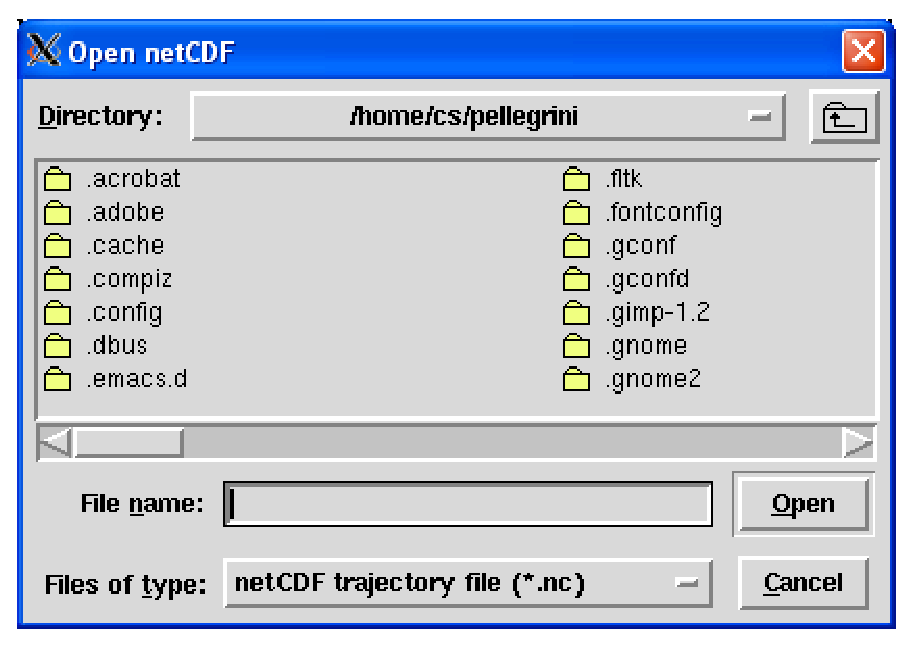
\includegraphics[width=10cm]{Figures/file_browser.eps}
\end{center}
\caption[File-Directory selection window]{File-Directory selection window.}
\label{fig:file_browser}
\end{figure}   

To select a directory, double click on it. By doing this, the complete pathname of the selected 
directory appears on the \textbf{Directory} selection button at the top of the window. To select
the parent directory left-click the directory selection button. When a file in the list is highlighted (clicked) 
its name is shown in the \textbf{File name} field. The selection is confirmed by pressing the button \textbf{Open} 
of the browser. By doing this, the file selection window closes.

Two kind of files can be loaded in \NMOLDYN, the \MMTK\ \NetCDF\ files and the \MMTK\ trajectory set 
files (usually with respective \textbf{.nc} and \textbf{.ncs} extensions), the latter being just an ASCII file where each 
line is a link to a \MMTK\ \NetCDF\ file. The figure \ref{fig:trajectory_set} shows an example of a trajectory set file. 
\begin{figure}[h!]
\begin{center}
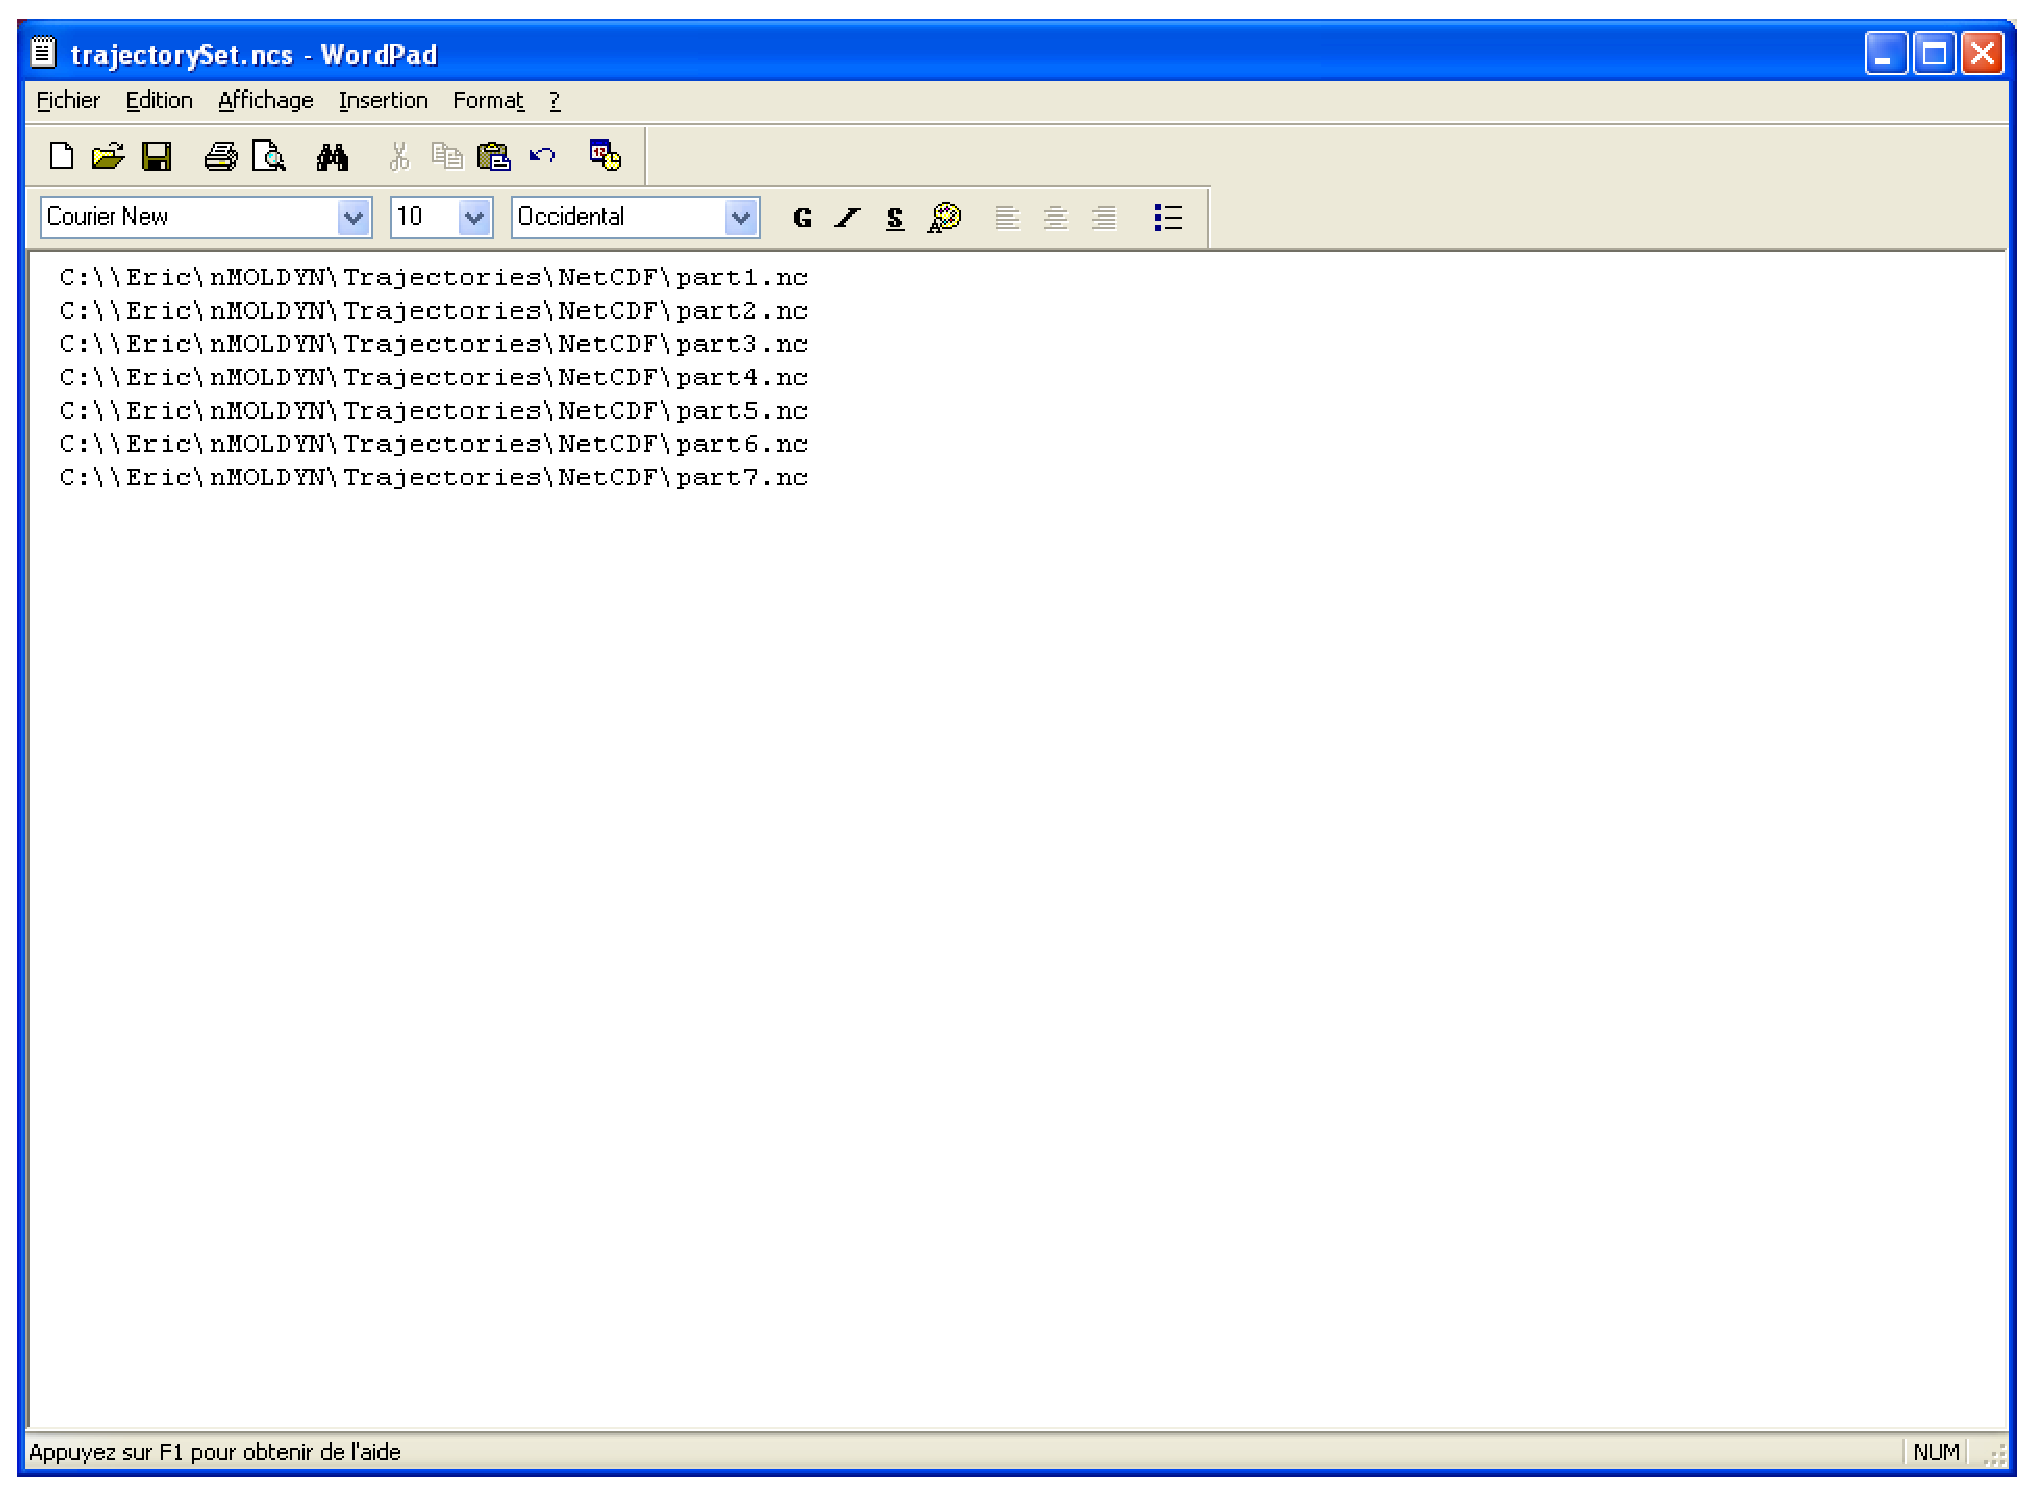
\includegraphics[width=10cm]{Figures/trajectory_set.eps}
\end{center}
\caption[Example of a MMTK trajectory set file]{Example of a MMTK trajectory set file.}
\label{fig:trajectory_set}
\end{figure}   

For more details about trajectory set files, please refer to the \MMTK\ documentation \cite{MMTK_TrajectorySet}.

Please note again that the \MMTK\ \NetCDF\ file format is central to \NMOLDYN\ as it is the only trajectory format that \NMOLDYN\ 
can handle directly. Trajectories that have not been produced with \MMTK\ or \MMTK -based programs must be converted 
to \MMTK\ format before they can be analyzed with \NMOLDYN.

One important step that is performed by \NMOLDYN\ when loading the trajectory is the determination of the chemical contents of 
the \MMTK\ universe corresponding to the loaded trajectory. \NMOLDYN\ attributes to each \MMTK\ chemical object found in 
the universe  a name that is either its \MMTK\ database name if this object is referenced in the \MMTK\ internal database 
otherwise its name will be its number of atoms appended to its chemical object type (respectively A, AC, M, NC, PC, P for Atom, 
AtomCluster, Molecule, NucleotideChain, PeptideChain, Protein chemical types.). In the seldom case where the system contains some isomers, 
\NMOLDYN\ will distinguish them by appending to their name the suffix \textbf{\_iso$i$}' where $i$ is the number of 
the isomer. In order to retrieve to which isomer corresponds the \NMOLDYN\ name, a PDB file whose name is the name of the isomer is created in the output file directory.

\subsection{Trajectory conversion}
\label{trajectory_conversion}
The \textbf{Trajectory conversion} option allows to convert a trajectory derived with a non \MMTK -based program to the \NetCDF\ \MMTK\ 
trajectory format. Pressing the button \textbf{Trajectory conversion} brings up a menu from which it is possible to choose 
the following trajectory converters:
\begin{itemize}
\item Amber NetCDF to MMTK
\item CHARMM/X-PLOR to MMTK
\item DL\_POLY to MMTK
\item MaterialsStudio
\item NAMD to MMTK
\item VASP to MMTK
\end{itemize}
Pressing the \textbf{MaterialsStudio} menubutton brings up an additional menu from which it is possible to choose the 
following Materials Studio converters:
\begin{itemize}
\item Discover module to MMTK
\item Forcite module to MMTK
\end{itemize}

\subsubsection{Amber to MMTK}
\label{amber_to_mmtk}
This converter allows the conversion from a \NetCDF\ trajectory generated with Amber 9 or 10 \cite{Amber} to a \MMTK\ \NetCDF\ trajectory 
(unfortunately, both \NetCDF\ files do not follow the same convention). For version of Amber lower than 9, Amber provides some tools 
for the conversion to Amber \NetCDF\ trajectories. Pressing the \textbf{Amber NetCDF to MMTK} menubutton, the dialog shown in 
figure \ref{fig:amber_converter} will pop up.
\newpage
\begin{figure}[h!]
\begin{center}
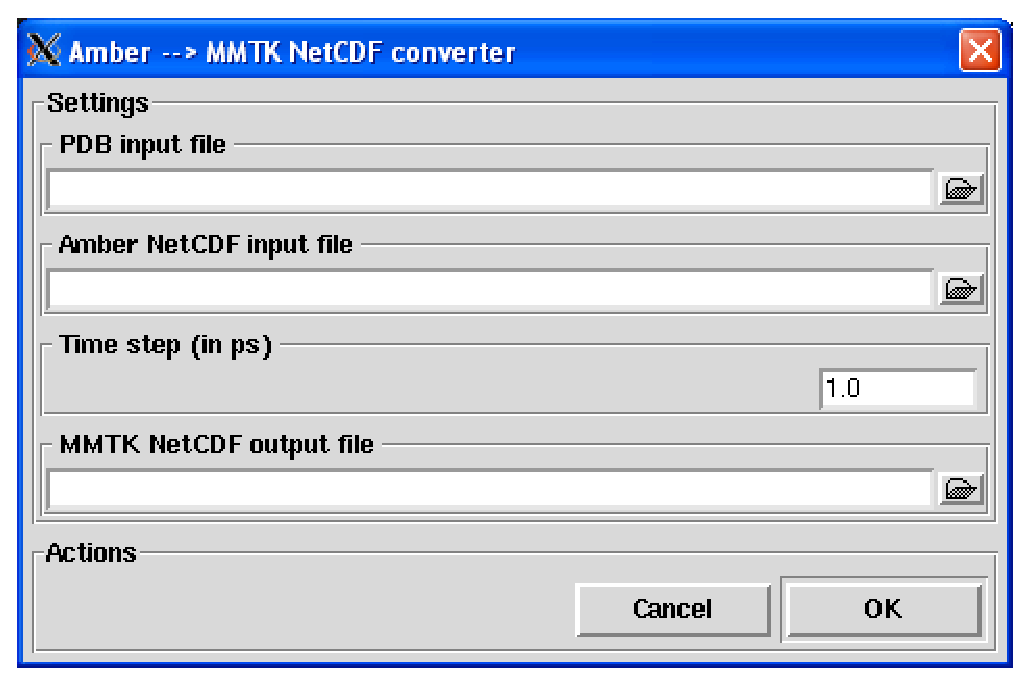
\includegraphics[width=10cm]{Figures/amber_converter.eps}
\end{center}
\caption[The Amber to MMTK converter dialog]{The Amber to MMTK converter dialog.}
\label{fig:amber_converter}
\end{figure}   

To perform the conversion, the following input fields must be filled:
\begin{itemize}
\item \textbf{PDB input file}\\
\textbf{Format:} string\\
\textbf{Default:} \textit{None}\\
\textbf{Description:} a PDB file of the system must be provided for the conversion. This file is necessary to build up the 
\MMTK\ universe related to the \MMTK\ trajectory. 

\item \textbf{Amber NetCDF input file}\\
\textbf{Format:} string\\
\textbf{Default:} \textit{None}\\
\textbf{Description:} the Amber 9 or 10 \NetCDF\ trajectory file that contains all the trajectory frames.

\item \textbf{Time step (in ps)}\\
\textbf{Format:} strictly positive float\\
\textbf{Default:} \textit{1.0}\\
\textbf{Description:} the time step in \ps\ between two consecutive frames of the Amber \NetCDF\ trajectory. You have to provide 
this information because it is not contained in the Amber \NetCDF\ trajectory file.

\item \textbf{MMTK NetCDF output file}\\
\textbf{Format:} string\\
\textbf{Default:} \textit{None}\\
\textbf{Description:} the name of the \MMTK\ \NetCDF\ trajectory that will be written. Once, an Amber \NetCDF\ 
file has been loaded, a default name for the \MMTK\ \NetCDF\ output file will be proposed. This default name will be 
\textit{file\_mmtk.nc} if \textit{file.nc} is the Amber \NetCDF\ trajectory file name.
\end{itemize}

\subsubsection{CHARMM/X-PLOR to MMTK}
\label{charmm_to_mmtk}
This converter allows the conversion from a trajectory generated with \CHARMM\ or X-PLOR \cite{CHARMM,X-PLOR} to a 
\MMTK\ \NetCDF\ trajectory. Pressing the \textbf{CHARMM/X-PLOR to MMTK} menubutton, the dialog shown in figure \ref{fig:charmm_converter} will pop up.
\begin{figure}[h!]
\begin{center}
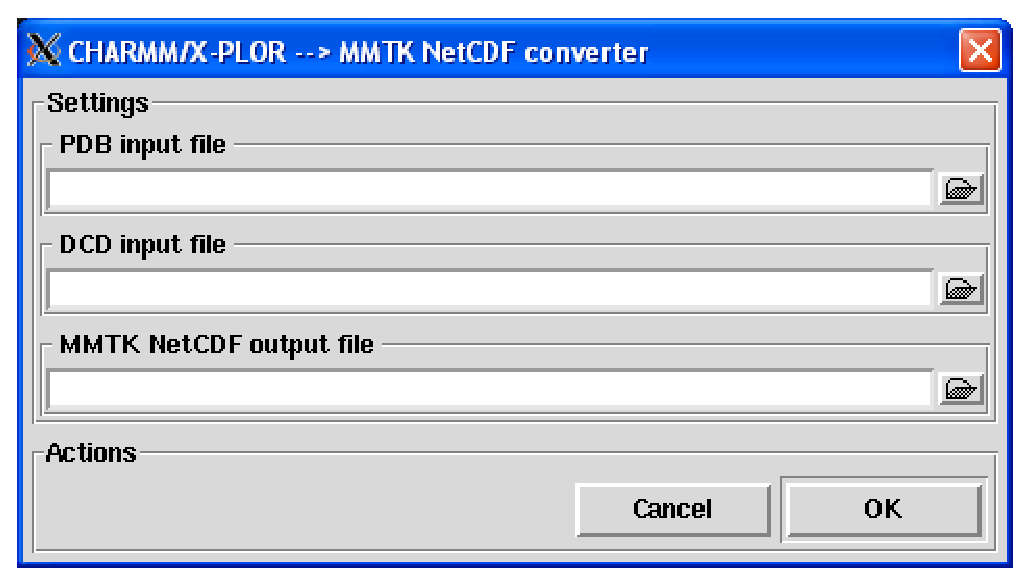
\includegraphics[width=10cm]{Figures/charmm_converter.eps}
\end{center}
\caption[The CHARMM to MMTK converter dialog]{The CHARMM to MMTK converter dialog.}
\label{fig:charmm_converter}
\end{figure}   

To perform the conversion, the following input fields must be filled:
\begin{itemize}
\item \textbf{PDB input file}\\
\textbf{Format:} string\\
\textbf{Default:} \textit{None}\\
\textbf{Description:} a PDB file of the system must be provided for the conversion. This file is necessary to build up 
the \MMTK\ universe related to the \MMTK\ trajectory. 

\item \textbf{DCD input file}\\
\textbf{Format:} string\\
\textbf{Default:} \textit{None}\\
\textbf{Description:} the \CHARMM\ DCD trajectory file that stores the trajectory frames.

\item \textbf{MMTK NetCDF output file}\\
\textbf{Format:} string\\
\textbf{Default:} \textit{None}\\
\textbf{Description:} the name of the \MMTK\ \NetCDF\ trajectory that will be written. Once, a DCD file has been 
loaded, a default name for the \MMTK\ \NetCDF\ output file will be proposed. This default name will be 
\textit{file.nc} if \textit{file.dcd} is the DCD trajectory file name.
\end{itemize}

\subsubsection{DL\_POLY to MMTK}
\label{dlpoly_to_mmtk}
This converter allows the conversion from a trajectory generated with DL\_POLY \cite{DL_POLY} to a \MMTK\ \NetCDF\ 
trajectory. Pressing the \textbf{DL\_POLY to MMTK} menubutton, the dialog shown in figure \ref{fig:dlpoly_converter} will pop up.
\newpage
\begin{figure}[h!]
\begin{center}
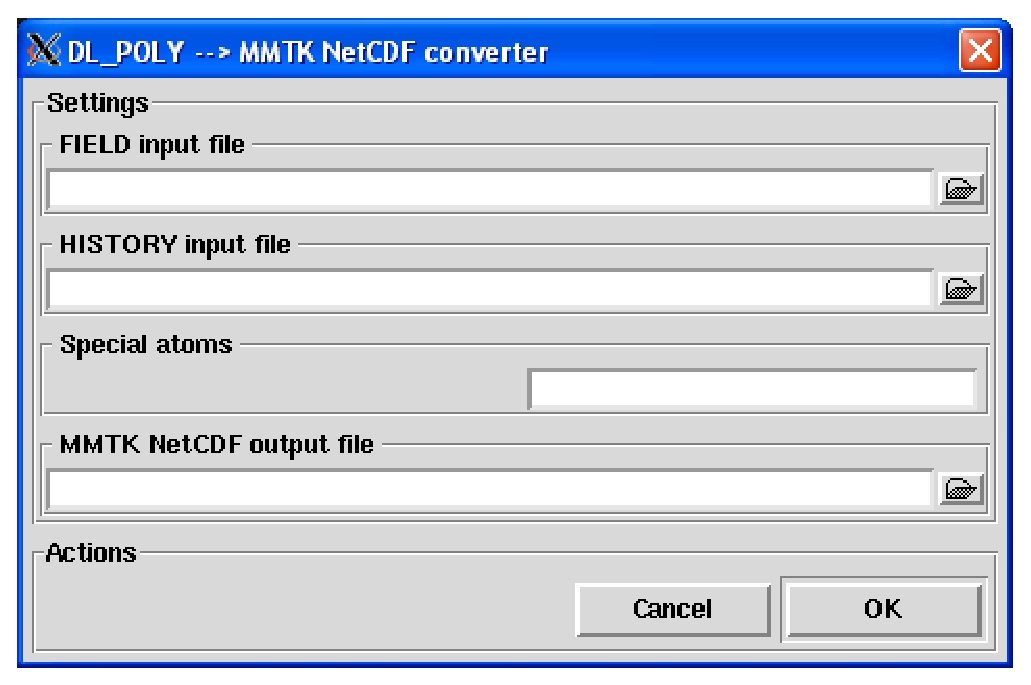
\includegraphics[width=10cm]{Figures/dlpoly_converter.eps}
\end{center}
\caption[The DL\_POLY to MMTK converter dialog]{The DL\_POLY to MMTK converter dialog.}
\label{fig:dlpoly_converter}
\end{figure}   

To perform the conversion, the following input fields must be filled:
\begin{itemize}
\item \textbf{FIELD input file}\\
\textbf{Format:} string\\
\textbf{Default:} \textit{None}\\
\textbf{Description:} the DL\_POLY FIELD file that stores the informations about the system. This file is necessary to build up 
the \MMTK\ universe related to the \MMTK\ trajectory.

\item \textbf{HISTORY input file}\\
\textbf{Format:} string\\
\textbf{Default:} \textit{None}\\
\textbf{Description:} the DL\_POLY HISTORY file that stores the trajectory frames.

\item \textbf{Special atoms}\\
\textbf{Format:} string\\
\textbf{Default:} \textit{None}\\
\textbf{Description:} \NMOLDYN\ will create the \MMTK\ universe with the atom names specified in the FIELD file. 
By default, \NMOLDYN\ will interpret these names directly as if they were a chemical symbol. If this fails, 
\NMOLDYN\ will remove the last character until it corresponds to a known chemical symbol. For example, an 
atom defined in the FIELD file as CB, will first be interpreted as an atom of chemical symbol CB. As it does not 
exist, \NMOLDYN\ will interpret it as an atom of chemical symbol C, namely a carbon atom. Usig htis procedure, 
it can happen that some atom names can be misunderstood or event not understood at all by \MMTK\. 
As an example, the figure \ref{fig:dlpoly_field_example} shows the example of a FIELD file 
where one carbon atom specification (the one in red in the figure) will be misinterpreted as a cesium atom.
\newpage
\begin{figure}[h!]
\begin{center}
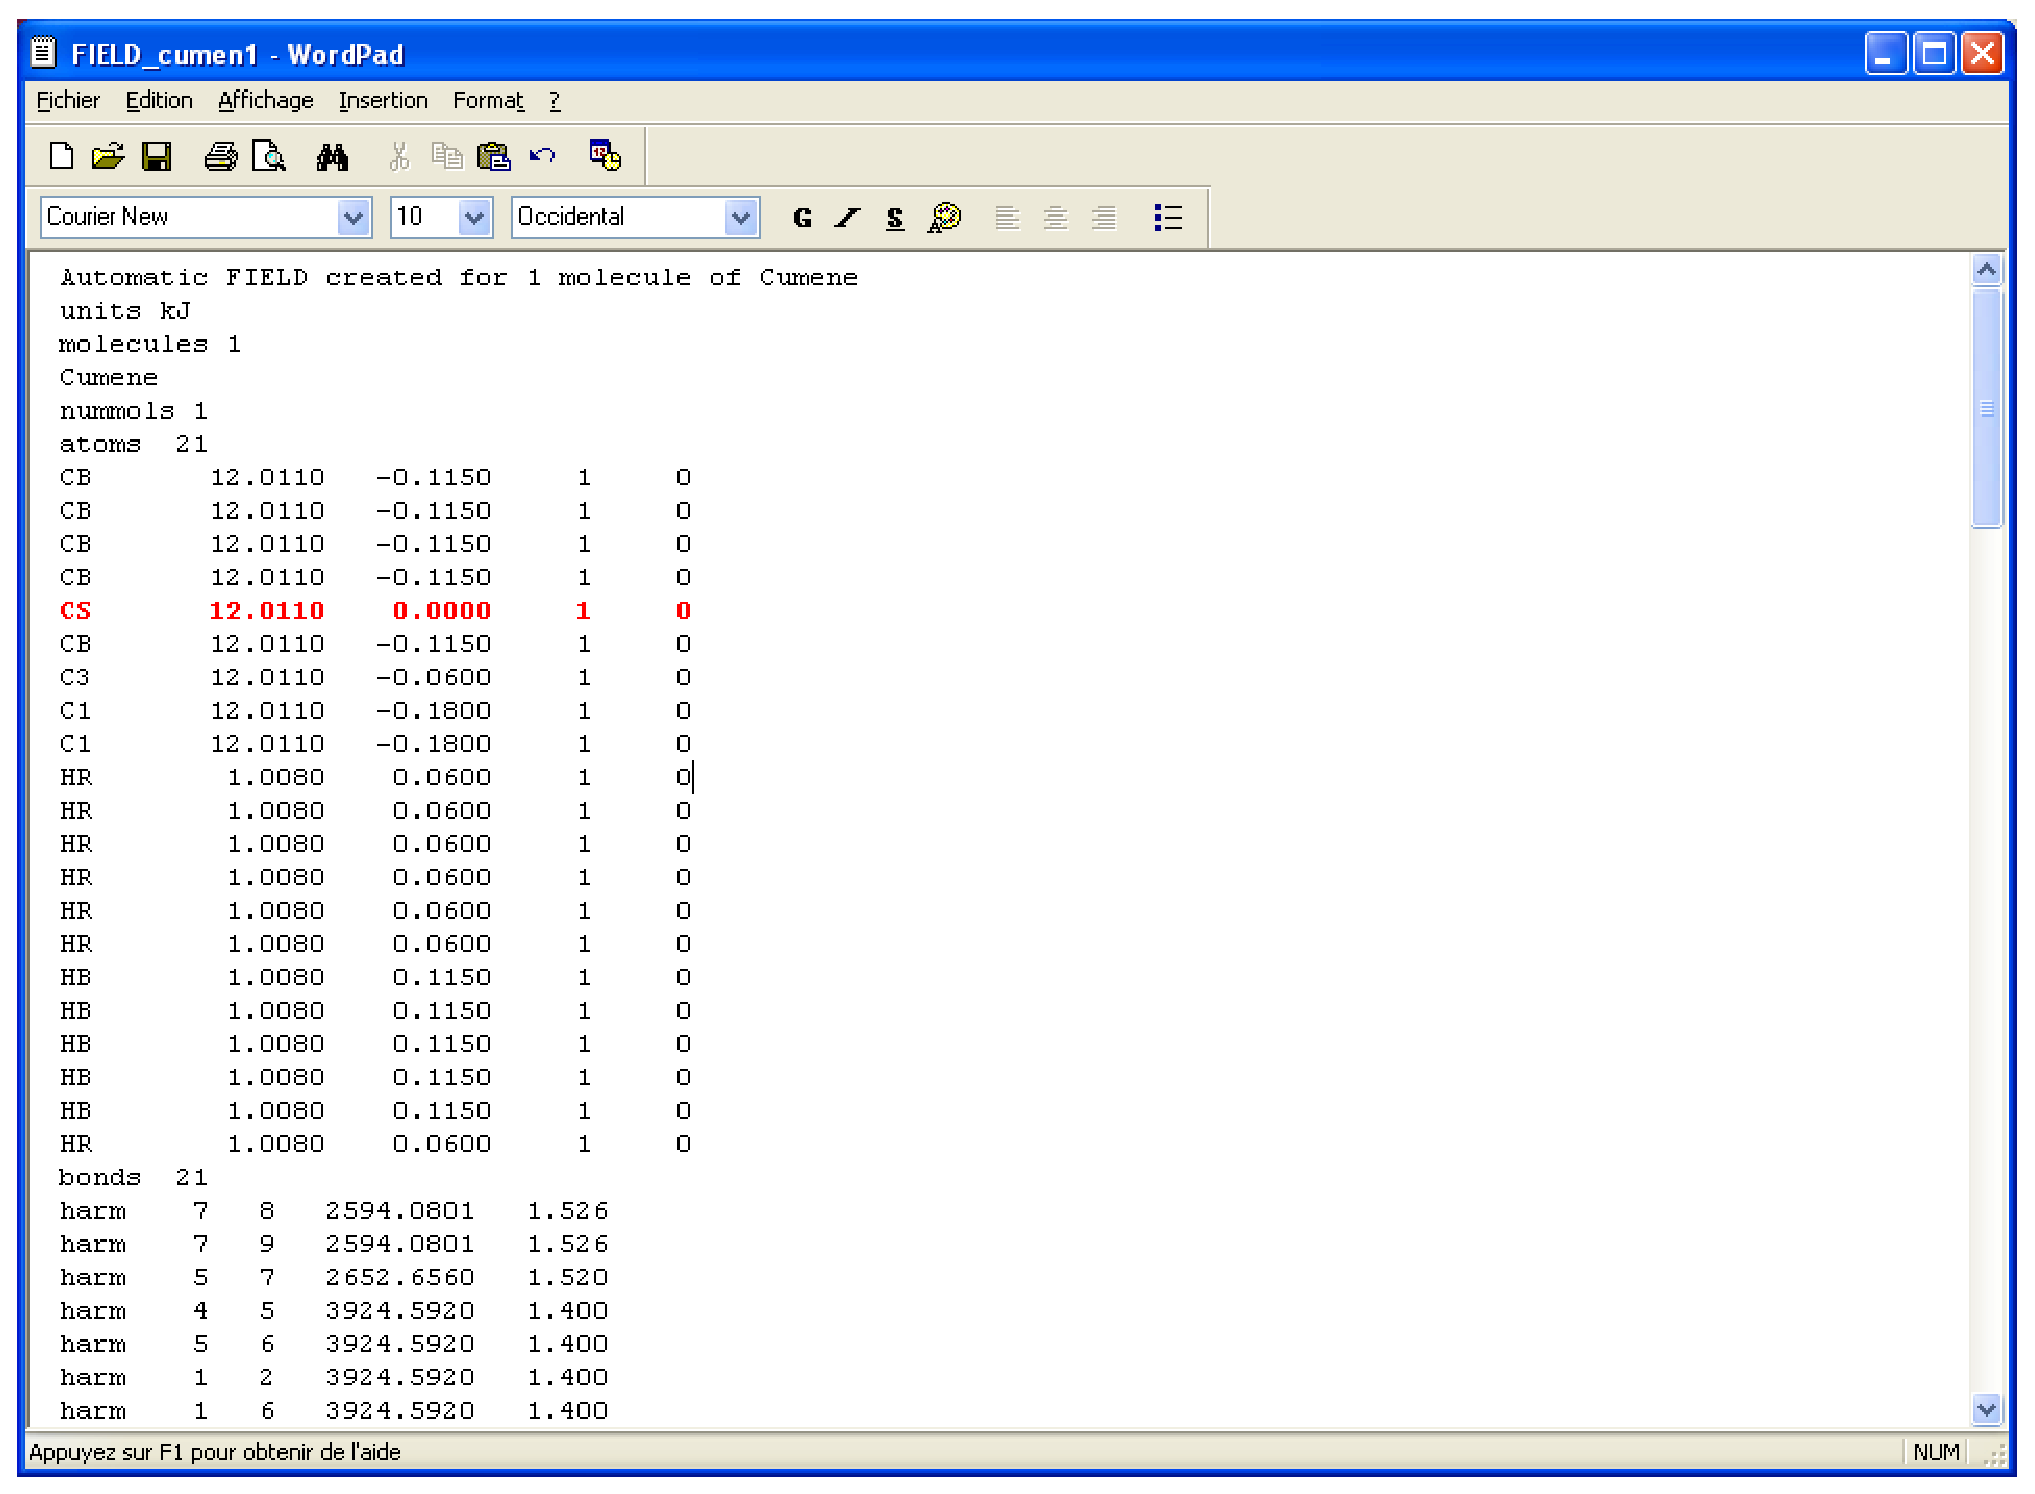
\includegraphics[width=10cm]{Figures/dlpoly_field_example.eps}
\end{center}
\caption[Example of a DL\_POLY/FIELD file]{Example of a DL\_POLY/FIELD file for which the \textbf{Special atoms} field must be 
filled because one carbon atom name, CS, will be interpreted as a cesium atom.}
\label{fig:dlpoly_field_example}
\end{figure}

The aim of the \textbf{Special atoms} field is precisely to avoid such problems. The format for the 
\textbf{Special atoms} field is
\\\\
\textit{atom name1:element1 sep atom name2:element2 \ldots} where \textit{sep} can be a white space, a comma or a semicolon.
\\\\
In the example showed in figure \ref{fig:dlpoly_field_example}, the string CS:C should be entered in the \textbf{Special atoms} field.
Interestingly, the \textbf{Special atoms} field can also be used to specify united atoms. The syntax is exactly the same but, in 
that case, the element name must be replaced by the \MMTK\ united atom code (e.g. CH3, CH2, CH, NH, NH2, NH3, OH, SH \ldots ).

\item \textbf{MMTK NetCDF output file}\\
\textbf{Format:} string\\
\textbf{Default:} \textit{None}\\
\textbf{Description:} the name of the \MMTK\ \NetCDF\ trajectory that will be written.
\end{itemize}

\subsubsection{Discover to MMTK}
\label{discover_to_mmtk}
This converter allows the conversion from a trajectory generated with MaterialsStudio Discover module \cite{Discover} to a 
\MMTK\ \NetCDF\ trajectory. Pressing the \textbf{Discover to MMTK} menubutton, the dialog shown in figure \ref{fig:discover_converter} will pop up.
\newpage
\begin{figure}[h!]
\begin{center}
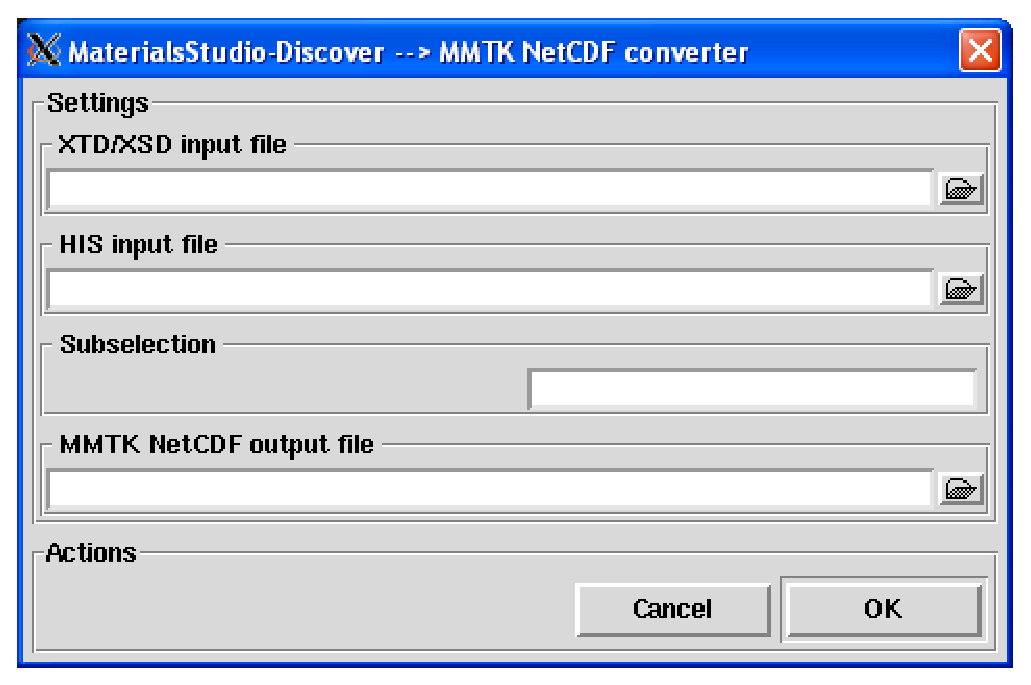
\includegraphics[width=10cm]{Figures/discover_converter.eps}
\end{center}
\caption[The Discover to MMTK converter dialog]{The Discover to MMTK converter dialog.}
\label{fig:discover_converter}
\end{figure}   

To perform the conversion, the following input fields must be filled:
\begin{itemize}
\item \textbf{XTD/XSD input file}\\
\textbf{Format:} string\\
\textbf{Default:} \textit{None}\\
\textbf{Description:} a XTD or XSD file of the system must be provided for the conversion. This file is necessary to build up 
the \MMTK\ universe related to the \MMTK\ trajectory. XTD or XSD files are automatically generated during a simulation performed 
with MaterialsStudio.

\item \textbf{HIS input file}\\
\textbf{Format:} string\\
\textbf{Default:} \textit{None}\\
\textbf{Description:} the Discover HIS file file that stores the trajectory frames.

\item \textbf{Subselection}:\\
\textbf{Format:} integer or Python expression or string\\
\textbf{Default:} \textit{None}\\
\textbf{Description:} it can happen that the molecular hierarchy is not correctly set in the XTD/XSD file or that 
you do not want to include all the atoms of the Discover trajectory into the \MMTK\ trajectory. In that case, 
it is possible to specify how the system should be organized.

The format for the \textbf{Subselection} field can be
\begin{itemize}
\item a single integer that specifies the index of the atom to select in the XSD/XTD file,
\item a valid python expression that will generate nested lists of integers where each list will generate a 
distinct \MMTK\ AtomCluster made of the atoms whose indexes in the XSD/XTD match the integers of the list. As an example, 
entering [[1,2,3,5],[10,20,21,23],[90,93]] will consider only atoms 1, 2, 3, 5, 10, 20, 21, 23, 90 and 93 of the XSD/XTD file when creating the \MMTK\ trajectory. Moreover, those atoms will be gathered 
such as atoms 1, 2, 3 and 5 will be in a fist AtomCluster, atoms 10, 20, 21 and 23 will be in a second AtomCluster and atoms 
90 and 93 will be gathered in a third AtomCluster,
\item a string with the following format:\\
\textit{min\_1:max\_1:skip\_1 sep \ldots\ sep min\_N:max\_N:skip\_N}\\
where \textit{sep} can be a white space, a comma or a semicolon and each block \textit{mini:maxi:skipi} will specify a 
distinct \MMTK\ AtomCluster made of atoms whose indexes in the XSD/XTD file ranges from \textit{min\_i} to \textit{max\_i} 
by jumps of \textit{skip\_i} atoms. For example, entering 2:5:1;20:30:3 will generate a first AtomCluster made of atoms 
2,3,4,5 and a second AtomCluster made of atoms 20,23,26 and 29.
\end{itemize}

\item \textbf{MMTK NetCDF output file}\\
\textbf{Format:} string\\
\textbf{Default:} \textit{None}\\
\textbf{Description:} the name of the \MMTK\ \NetCDF\ trajectory that will be written. Once, a HIS has been 
loaded, a default name for the \MMTK\ \NetCDF\ output file will be proposed. This default name will be 
\textit{file.nc} if \textit{file.his} is the HIS trajectory file name.
\end{itemize}

\subsubsection{Forcite to MMTK}
\label{forcite_to_mmtk}
This converter allows the conversion from a trajectory generated with Materials Studio Forcite module \cite{Forcite} to a 
\MMTK\ \NetCDF\ trajectory file. Pressing the \textbf{Forcite to \MMTK\ } menubutton, the dialog shown in figure \ref{fig:forcite_converter} will pop up.
\begin{figure}[h!]
\begin{center}
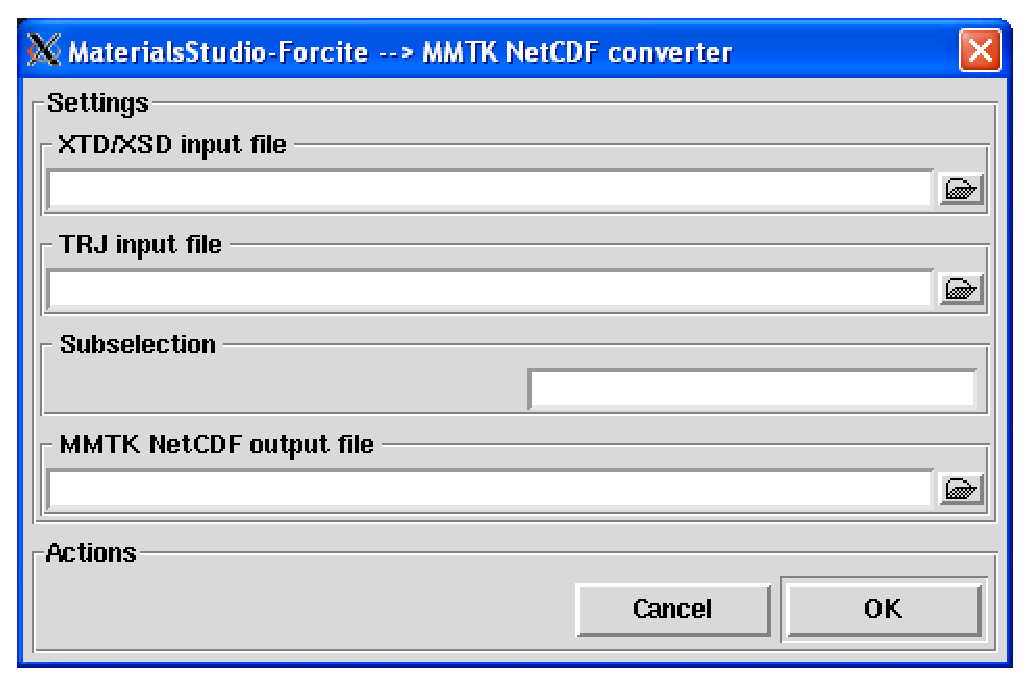
\includegraphics[width=10cm]{Figures/forcite_converter.eps}
\end{center}
\caption[The Forcite to MMTK converter dialog]{The Forcite to MMTK converter dialog.}
\label{fig:forcite_converter}
\end{figure}   

To perform the conversion, the following input fields must be filled:
\begin{itemize}
\item \textbf{XTD/XSD input file}\\
\textbf{Format:} string\\
\textbf{Default:} \textit{None}\\
\textbf{Description:} a XTD or XSD file of the system must be provided for the conversion. This file is necessary to build up 
the \MMTK\ universe related to the \MMTK\ trajectory. XTD or XSD files are automatically generated during a simulation performed 
with MaterialsStudio.

\item \textbf{TRJ input file}\\
\textbf{Format:} string\\
\textbf{Default:} \textit{None}\\
\textbf{Description:} the Forcite TRJ file that stores the trajectory frames.

\item \textbf{Subselection}:\\
\textbf{Format:} integer or Python expression or string\\
\textbf{Default:} \textit{None}\\
\textbf{Description:} it can happen that the molecular hierarchy is not correctly set in the XTD/XSD file or that 
you do not want to include all the atoms of the Discover trajectory into the \MMTK\ trajectory. In that case, 
it is possible to specify how the system should be organized.

The format for the \textbf{Subselection} field can be
\begin{itemize}
\item a single integer that specifies the index of the atom to select in the XSD/XTD file,
\item a valid python expression that will generate nesteds list of integers where each list will generate a 
distinct \MMTK\ AtomCluster made of the atoms whose indexes in the XSD/XTD match the integers of the list. As an example, 
entering [[1,2,3,5],[10,20,21,23],[90,93]] will consider only atoms 1, 2, 3, 5, 10, 20, 21, 23, 90 and 93 of the XSD/XTD file when creating the \MMTK\ trajectory. Moreover, those atoms will be gathered 
such as atoms 1, 2, 3 and 5 will be in a fist AtomCluster, atoms 10, 20, 21 and 23 will be in a second AtomCluster and atoms 
90 and 93 will be gathered in a third AtomCluster,
\item a string with the following format:\\
\textit{min\_1:max\_1:skip\_1 sep \ldots\ sep min\_n:max\_n:skip\_n}\\
where \textit{sep} can be a white space, a comma or a semicolon and each block \textit{min\_i:max\_i:skip\_i} will specify a distinct \MMTK\ AtomCluster made of atoms 
whose indexes in the XSD/XTD file ranges from \textit{min\_i} to \textit{max\_i} by jumps of \textit{skip\_i} atoms. For example, entering 2:5:1;20:30:3 will generate a first AtomCluster made of atoms 2,3,4,5 and a second AtomCluster made of atoms 20,23,26 and 29.
\end{itemize}

\item \textbf{MMTK NetCDF output file}\\
\textbf{Format:} string\\
\textbf{Default:} \textit{None}\\
\textbf{Description:} the name of the \MMTK\ \NetCDF\ trajectory that will be written. Once, a TRJ file has been 
loaded, a default name for the \MMTK\ \NetCDF\ output file will be proposed. This default name will be 
\textit{file.nc} if \textit{file.trj} is the TRJ trajectory file name.
\end{itemize}

\subsubsection{NAMD to MMTK}
\label{namd_to_mmtk}
This converter allows the conversion from a trajectory generated with \NAMD\ \cite{NAMD} to a \MMTK\ \NetCDF\ trajectory. 
Pressing the \textbf{NAMD to MMTK} menubutton, the dialog shown in figure \ref{fig:namd_converter} will pop up.
\newpage
\begin{figure}[h!]
\begin{center}
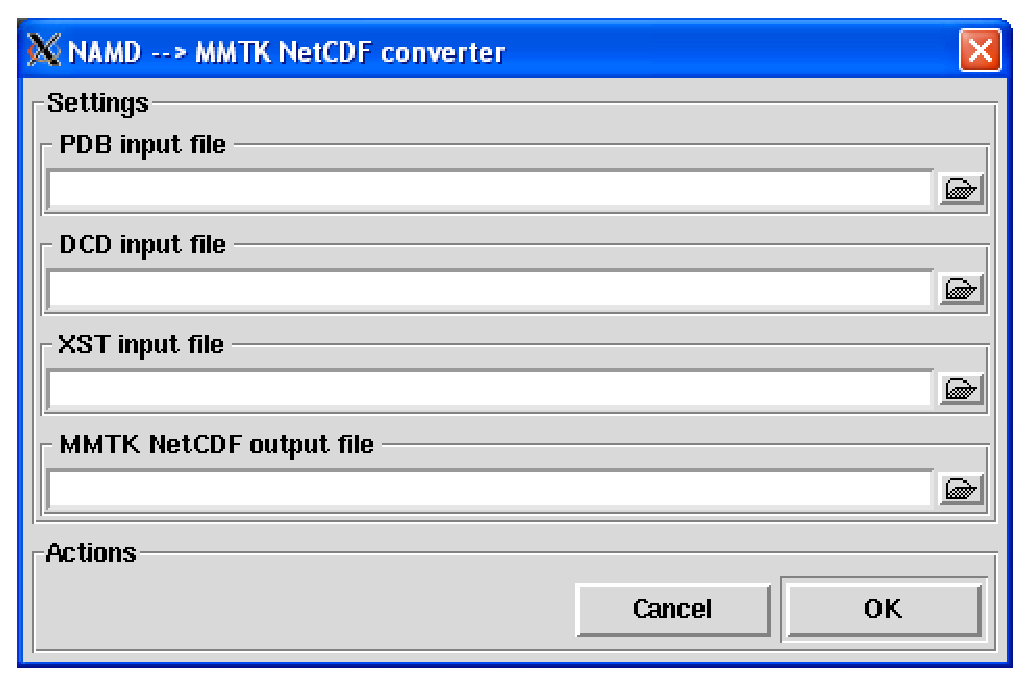
\includegraphics[width=10cm]{Figures/namd_converter.eps}
\end{center}
\caption[The NAMD to MMTK converter dialog]{The NAMD to MMTK converter dialog.}
\label{fig:namd_converter}
\end{figure}   

To perform the conversion, the following input fields must be filled:
\begin{itemize}
\item \textbf{PDB input file}\\
\textbf{Format:} string\\
\textbf{Default:} \textit{None}\\
\textbf{Description:} a PDB file of the system must be provided for the conversion. This file is necessary to build up 
the \MMTK\ universe related to the \MMTK\ trajectory. 

\item \textbf{DCD input file}\\
\textbf{Format:} string\\
\textbf{Default:} \textit{None}\\
\textbf{Description:} the \CHARMM\ DCD trajectory file that stores the trajectory frames.

\item \textbf{XST input file}:\\
\textbf{Format:} string\\
\textbf{Default:} \textit{None}\\
\textbf{Description:} The \NAMD\ \XST\ file has to be provided to the converter.

\item \textbf{MMTK NetCDF output file}\\
\textbf{Format:} string\\
\textbf{Default:} \textit{None}\\
\textbf{Description:} the name of the \MMTK\ \NetCDF\ trajectory that will be written. Once, a DCD file has been 
loaded, a default name for the \MMTK\ \NetCDF\ output file will be proposed. This default name will be 
\textit{file.nc} if \textit{file.dcd} is the DCD trajectory file name.
\end{itemize}

\subsubsection{VASP to MMTK}
\label{vasp_to_mmtk}
This converter allows the conversion from a trajectory generated with \VASP\ \cite{VASP} to a \MMTK\ \NetCDF\ trajectory. 
Pressing the \textbf{VASP to MMTK} menubutton, the dialog shown in figure \ref{fig:vasp_converter} will pop up.
\begin{figure}[h!]
\begin{center}
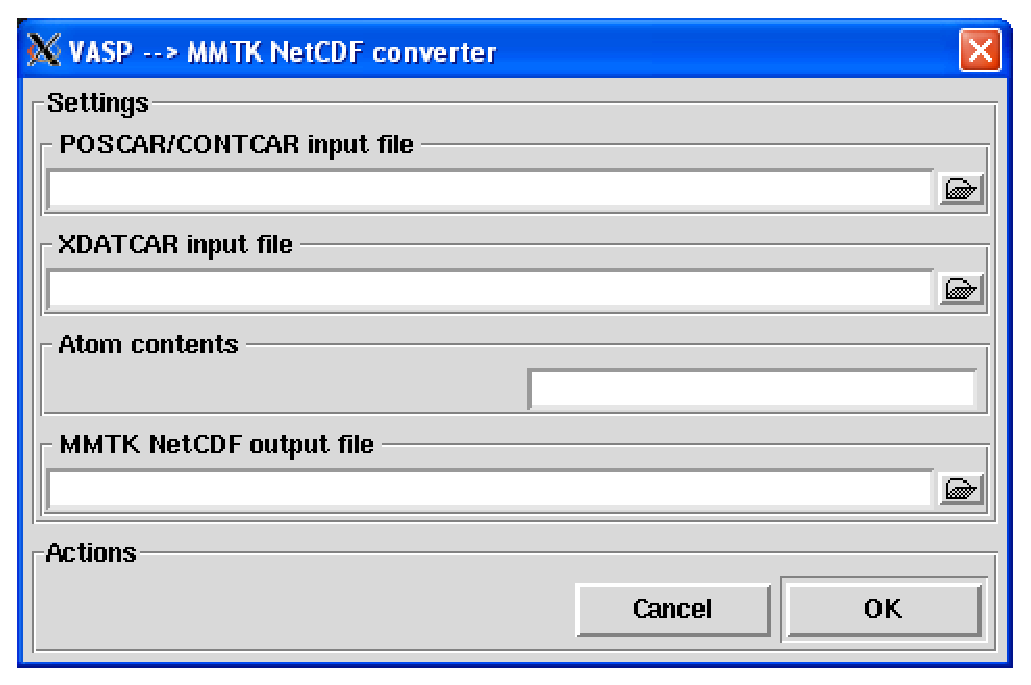
\includegraphics[width=10cm]{Figures/vasp_converter.eps}
\end{center}
\caption[The VASP to MMTK converter dialog]{The VASP to MMTK converter dialog.}
\label{fig:vasp_converter}
\end{figure}   

To perform the conversion, the following input fields must be filled:
\begin{itemize}
\item \textbf{CONTCAR/POSCAR input file}\\
\textbf{Format:} string\\
\textbf{Default:} \textit{None}\\
\textbf{Description:} the \VASP\ CONTCAR or POSCAR file that stores the informations about the system. This file is 
necessary to build up the \MMTK\ universe related to the \MMTK\ trajectory.

\item \textbf{XDATCAR input file}\\
\textbf{Format:} string\\
\textbf{Default:} \textit{None}\\
\textbf{Description:} the \VASP\ XDATCAR file that stores the trajectory frames.

\item \textbf{Atom contents}\\
\textbf{Format:} string\\
\textbf{Default:} \textit{None}\\
\textbf{Description:} the CONTCAR file contains the number of atoms of each element in the system but does not tell the elements the system is 
made of. This information has to provided using the \textbf{Atom contents} field. 

The format for the \textbf{Atom contents} field is
\\\\
\textit{element1 sep element2 \ldots } where \textit{sep} can be a white space, a comma or a semicolon and 
\textit{element1, elemnt2} \ldots are the chemical symbols of element 1, 2 \ldots
\\\\
Interestingly, the \textbf{Atom contents} field can also be used to specify united atoms. The syntax is exactly the same but, in 
that case, the element name must be replaced by the \MMTK\ united atom code (e.g. CH3, CH2, CH, NH, NH2, NH3, OH, S \ldots ).

\item \textbf{MMTK NetCDF output file}\\
\textbf{Format:} string\\
\textbf{Default:} \textit{None}\\
\textbf{Description:} the name of the \MMTK\ \NetCDF\ trajectory that will be written.
\end{itemize}

\subsection{Frame snapshot}
\label{frame_snapshot}
The \textbf{Frame snapshot} option allows the extraction of one or several frames in \PDB\ format from a \MMTK\ \NetCDF\ 
trajectory. Clicking on it, the dialog shown in figure \ref{fig:frame_snapshot} will pop up.
\begin{figure}[h!]
\begin{center}
\includegraphics[width=10cm]{Figures/frame_snapshot.eps}
\end{center}
\caption[The frame extraction dialog]{The dialog used to export trajectory frames to a PDB file.}
\label{fig:frame_snapshot}
\end{figure}   

To perform the frame extraction, the following input fields must be filled:
\begin{itemize}
\item \textbf{NetCDF input file}\\
\textbf{Format:} string\\
\textbf{Default:} \textit{None}\\
\textbf{Description:} a \MMTK\ \NetCDF\ trajectory file of the system must be provided for the extraction. 
If a trajectory is currently loaded, it will be proposed by default for the frame extraction.

\item \textbf{Selected frames}\\
\textbf{Format:} integer or Python expression or string\\
\textbf{Default:} \textit{1}\\
\textbf{Description:} this field will store the frames selected for extraction. The format for the \textbf{Selected frames} 
field can be:
\begin{itemize}
\item an integer specifying the index of a single frame to extract
\item a valid Python expression that will generate a list of integers where each integer specify the index of a frame to extract.
\item a string with the following format:\\
\textit{min 1:max 1:skip 1 sep \ldots\ sep min N:max N:skip N}\\
where \textit{sep} can be a white space, a comma or a semicolon and each block \textit{min i:max i:skip i} will specify a 
range of frames including frame \textit{min i} to frame \textit{max i} by jump of \textit{skip i} frames.
\end{itemize}

\item \textbf{PDB output file}\\
\textbf{Format:} string\\
\textbf{Default:} \textit{None}\\
\textbf{Description:} this field will store the name of the \PDB\ output file that will contain the extracted frames. The line
\\\\
\textit{REMARK Frame i}
\\\\
will be written before each written frame \textit{i}.
\end{itemize}

\subsection{Convert NetCDF to ASCII}
\label{convert_netcdf_ascii}
The \textbf{Convert NetCDF to ASCII} option allows the conversion of any kind of \NetCDF\ file to a \CDL\ file \cite{CDL}. 
Clicking on it, the dialog shown in figure \ref{fig:convert_netcdf_ascii} will pop up. 
\begin{figure}[h!]
\begin{center}
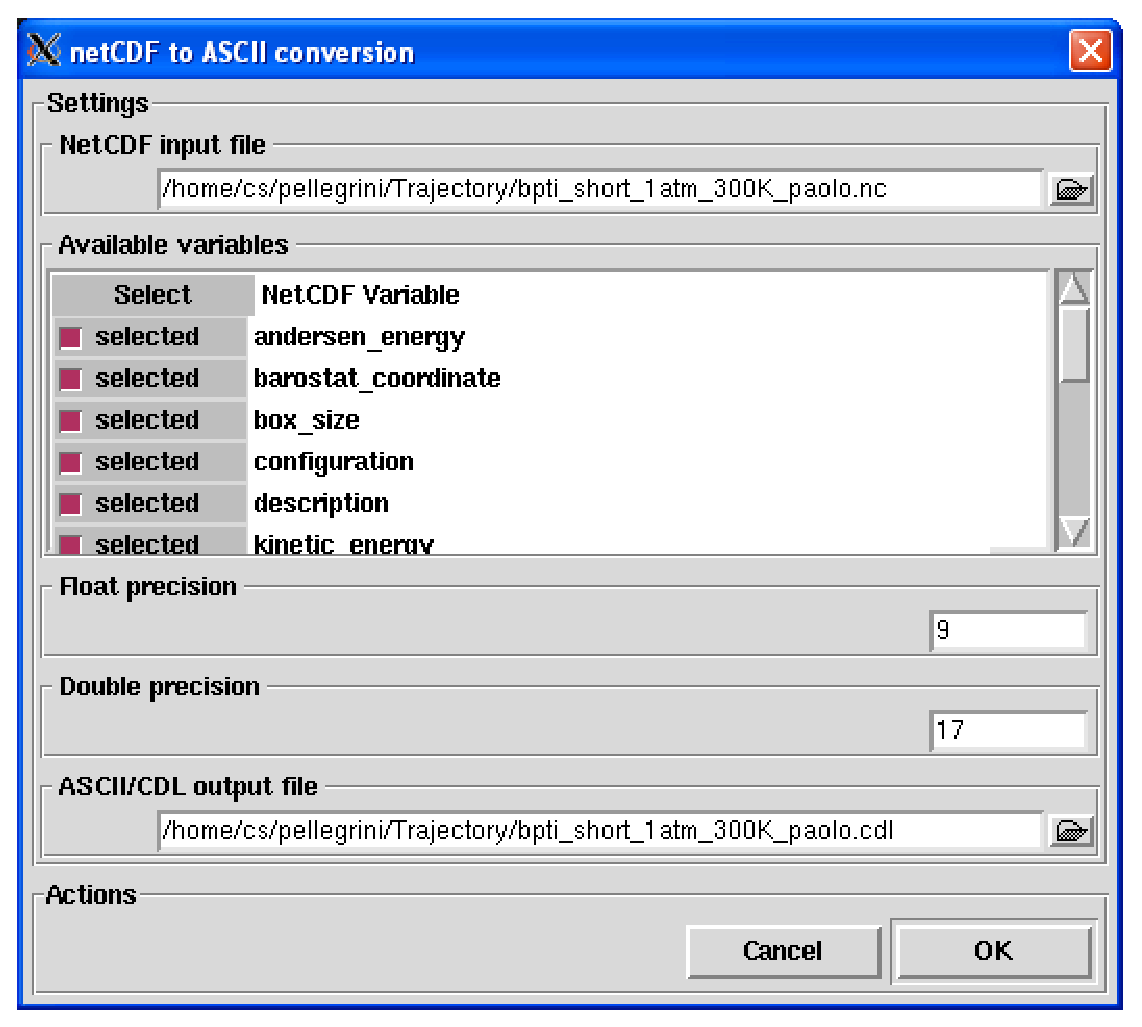
\includegraphics[width=10cm]{Figures/convert_netcdf_ascii.eps}
\end{center}
\caption[The NetCDF to ASCII conversion dialog]{The dialog used to convert files in NetCDF format to CDL format.}
\label{fig:convert_netcdf_ascii}
\end{figure}   

To use this functionnality, the \textbf{ncdump} program \cite{ncdump} provided with the \NetCDF\ library must be installed and the path to the 
\textbf{ncdump} executable must be defined in the \NMOLDYN\ preferences. If \textbf{ncdump} is not installed, 
this functionnality will be disabled.

To perform the conversion, the following input fields must be filled:
\begin{itemize}
\item \textbf{NetCDF file}\\
\textbf{Format:} string\\
\textbf{Default:} \textit{None}\\
\textbf{Description:} a \NetCDF\ file must be provided for the conversion. If a \NetCDF\ file is currently loaded (a \MMTK\ 
trajectory or other kind of \NetCDF\ file), it will be proposed by default for conversion. Once the \NetCDF\ file is loaded 
all the variables found in the \NetCDF\ file will be displayed in the \textbf{Available variables} field.

\item \textbf{Available variables}\\
\textbf{Format:} Not an editable field\\
\textbf{Default:} \textit{None}\\
\textbf{Description:} this field displays all the variables contained in the \NetCDF\ file. It contains two columns: 
the first one displays the checkbuttons that will allow to unselect/select which \NetCDF\ variable (displayed on the right column) 
should be considered for conversion.

\item \textbf{Float precision}\\
\textbf{Format:} integer\\
\textbf{Default:} \textit{9}\\
\textbf{Description:} this field stores the precision at which floating numbers will be written in the ASCII/CDL output file.

\item \textbf{Double precision}\\
\textbf{Format:} integer\\
\textbf{Default:} \textit{17}\\
\textbf{Description:} this field stores the precision at which double numbers will be written in the ASCII/CDL output file.

\item \textbf{ASCII/CDL output file}\\
\textbf{Format:} string\\
\textbf{Default:} \textit{None}\\
\textbf{Description:} this field stores the name of the ASCII/CDL output file.\\
\end{itemize}

\subsection{Convert ASCII to NetCDF}
\label{convert_ascii_netcdf}
The \textbf{Convert ASCII to NetCDF} option allows the conversion of from an ASCII file to a \NetCDF\ file. 
Clicking on it, the dialog shown in figure \ref{fig:convert_ascii_netcdf} will pop up. 
\newpage
\begin{figure}[h!]
\label{fig:convert_ascii_netcdf}
\begin{center}
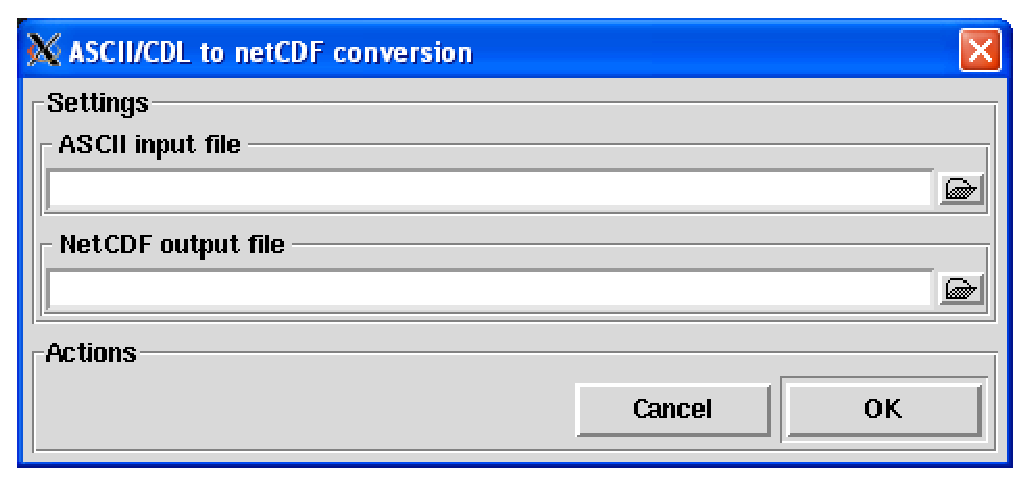
\includegraphics[width=10cm]{Figures/convert_ascii_netcdf.eps}
\end{center}
\caption[The ASCII to NetCDF conversion dialog]{The dialog used to convert files in ASCII/CDL format to NetCDF format.}
\end{figure}   

To use this functionnality, the \textbf{ncgen} program \cite{ncgen} provided with the \NetCDF\ library must be 
installed and the path to the \textbf{ncgen} executable must be defined in the \NMOLDYN\ preferences. 
If \textbf{ncgen} is not installed, this functionnality will be disabled.

To perform the conversion, the following input fields must be filled:
\begin{itemize}
\item \textbf{ASCII input file}\\
\textbf{Format:} string\\
\textbf{Default:} \textit{None}\\
\textbf{Description:} this field stores the name of the ASCII input file that will be used for the conversion. Two possible 
ASCII file formats are compatible for the conversion. The first one is the \CDL\ file format \cite{CDL} and the second one is 
a simpler but less general format where only numeric data can be converted. The latter format must contain white spaces separated columns where 
each column will be interpreted as a \NetCDF\ unidimensional array of double. The file can contain header lines that must 
start with '\#' character. The rest of the line will be stored in the \NetCDF\ global attribute 'comment'. 
Some \NetCDF\ global variables can also be specified for the conversion. They must be declared one after the other inside 
the header using the following format;
\\\\
\textit{\# global name = value}
\\\\
Finally, a name and some additional \NetCDF\ variable attributes (units \ldots ) can be given to the columns that will 
be converted. Column names must be declared one after the other inside the header using the following format:
\\\\
\textit{\# variable name = value ; attribute1 = value1 ; attribute2 = value2 ...}
\\\\
In such a case the number of variable declaration must be exactly the same than the number of columns. Otherwise the 
\NetCDF\ variable name will be Column\textit{i} where \textit{i} is the column index.

The figure \ref{fig:convert_ascii_netcdf_example} shows an example of such file.
\newpage
\begin{figure}[h!]
\begin{center}
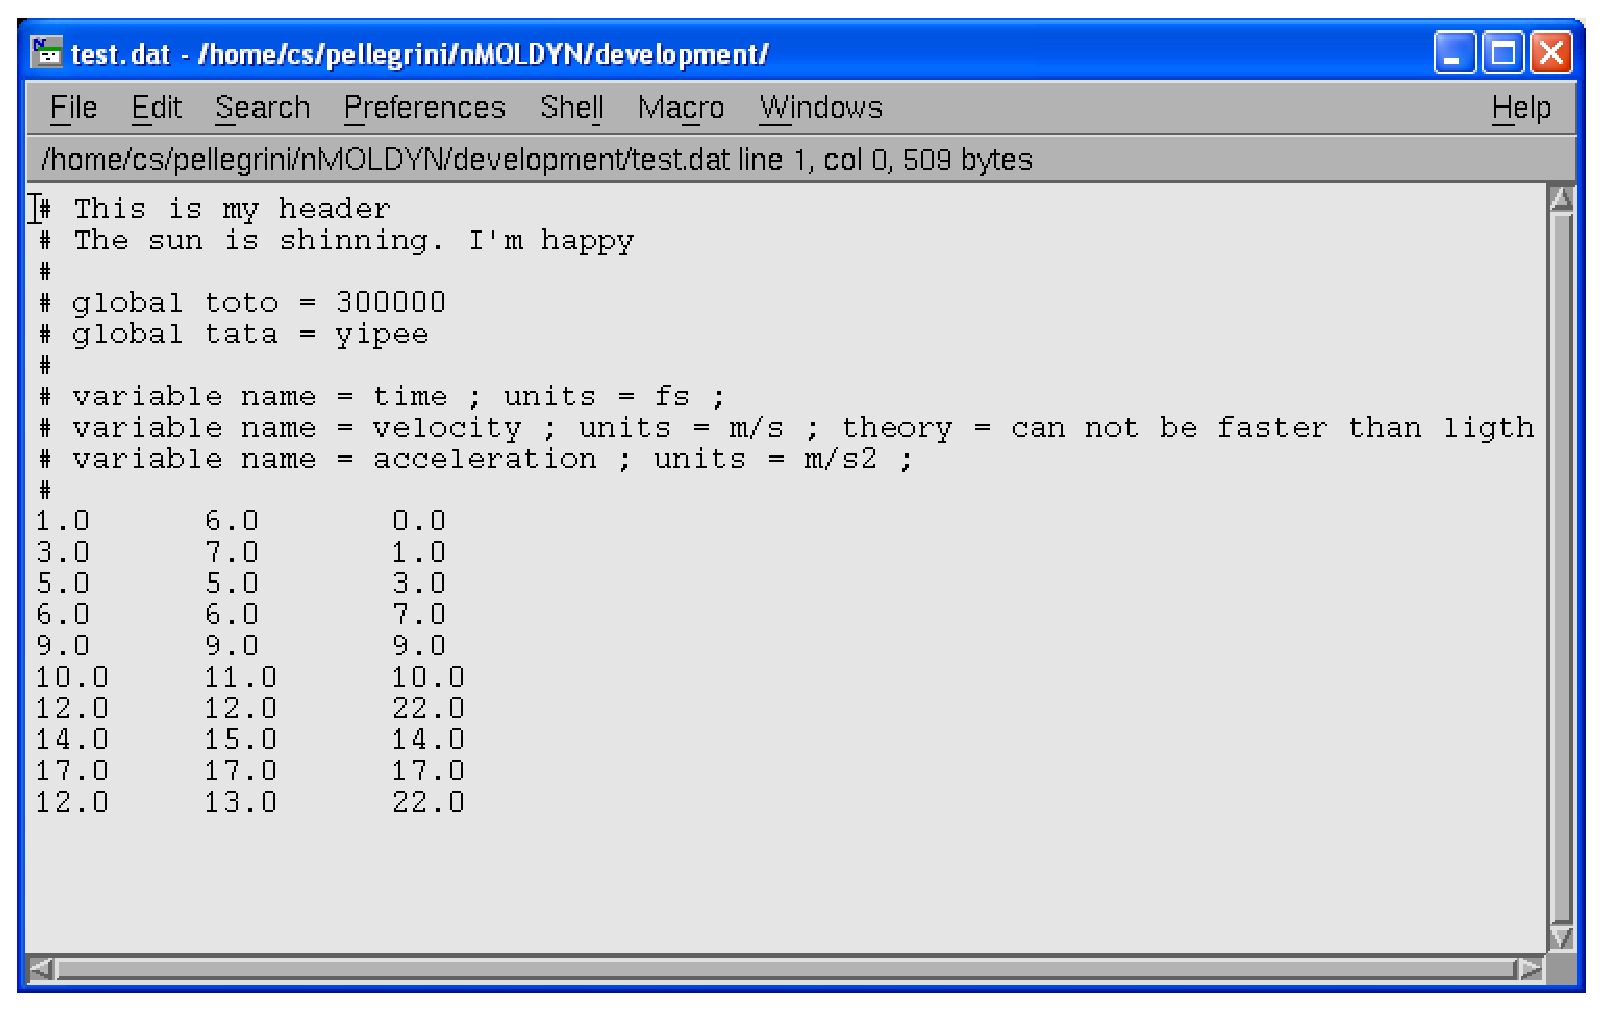
\includegraphics[width=10cm]{Figures/convert_ascii_netcdf_example.eps}
\end{center}
\caption[Example of an ASCII file that can be converted to a NetCDF file]{Example of an ASCII file that can be converted to a NetCDF file.}
\label{fig:convert_ascii_netcdf_example}
\end{figure}   

The output \NetCDF\ file resulting from its conversion will contain:
\begin{itemize}
\item a NetCDF dimension 'nvalues' whose value corresponds to the length of the columns to convert (in that case 10),
\item a global attribute 'comment' whose value is ' The sun is shinning. I'm happy',
\item a global attribute 'toto' whose value is '300000',
\item a global attribute 'tata' whose value is 'yipee',
\item a NetCDF variable 'time' of dimension 'nvalues' with an additional attribute 'units' whose value is 'fs',
\item a NetCDF variable 'velocity' of dimension 'nvalues' with additional attributes 'units' and 'theory' whose values are respectively 
'm/s' and 'can not be faster than light',
\item a NetCDF variable 'acceleration' of dimension 'nvalues' with an additional attribute 'units' whose value is 'm/s2',
\end{itemize}

\item \textbf{NetCDF output file}\\
\textbf{Format:} string\\
\textbf{Default:} \textit{None}\\
\textbf{Description:} this field stores the name of the \NetCDF\ output file.
\end{itemize}

\subsection{Preferences}
\label{preferences}
The \textbf{Preferences} option allows to set the \NMOLDYN\ preferences using the \textbf{ConfigParser} Python-module mechanism 
\cite{ConfigParser}. In \NMOLDYN\, the preferences are classified in the three following sections:
\begin{itemize}
\item File handling: contains the preferences variables related to the file handled by \NMOLDYN\ (log file, output file \ldots ),
\item External programs: contains the preferences variables related to the actions performed by \NMOLDYN\ that require 
an external program (e.g. displaying the documentation, animating a trajectory, converting \NetCDF\ to ASCII or ASCII 
to \NetCDF\ \ldots ),
\item Miscellaneous: contains the other preferences variables that could not be classified elssewhere.
\end{itemize}
Pressing the \textbf{Preferences} menubutton will pop up the dialog shown in figure \ref{fig:preferences_file_handling}. 
\begin{figure}[h!]
\begin{center}
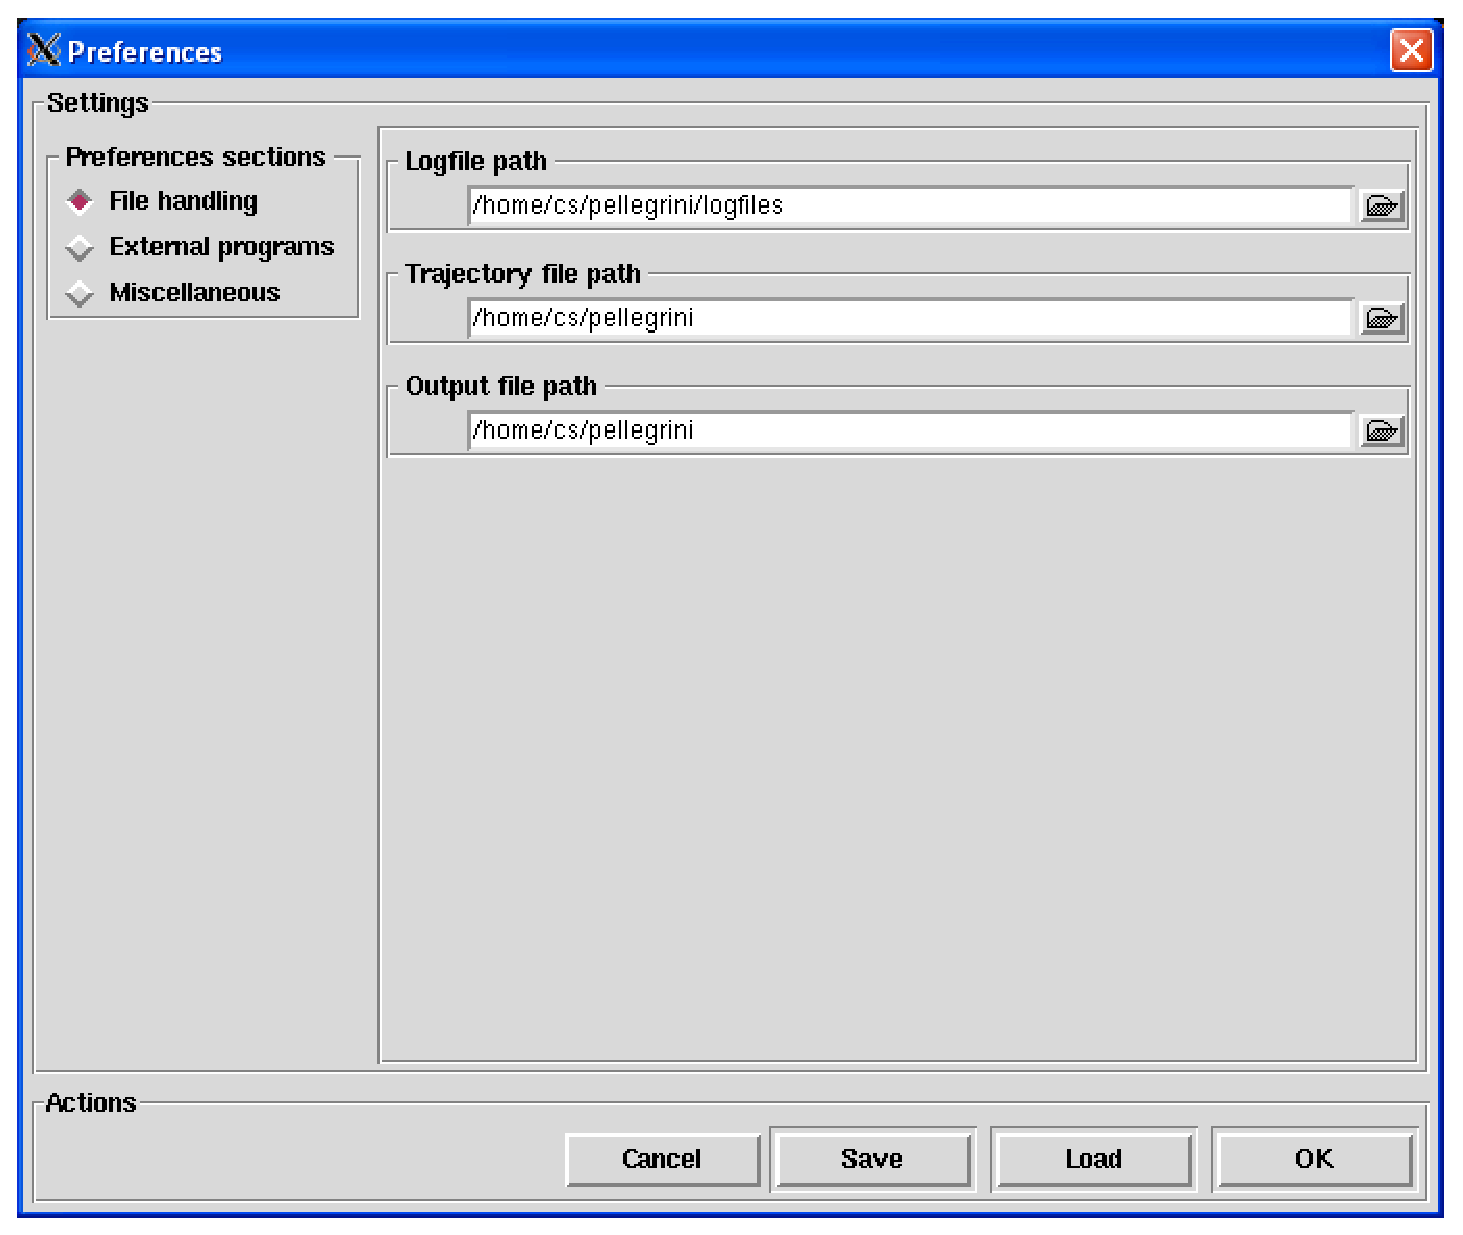
\includegraphics[width=10cm]{Figures/preferences_file_handling.eps}
\end{center}
\caption[The Preferences dialog]{The dialog used to set up \NMOLDYN\ preferences.}
\label{fig:preferences_file_handling}
\end{figure}   

By default, the dialog for \textbf{File handling} section is displayed. Clicking on the \textbf{File handling}, 
\textbf{External programs} or \textbf{Miscellaneous} radiobutton will display the dialog corresponding to the selected 
section (see Figure \ref{fig:preferences_sections}).
\begin{figure}[h!]
\begin{center}
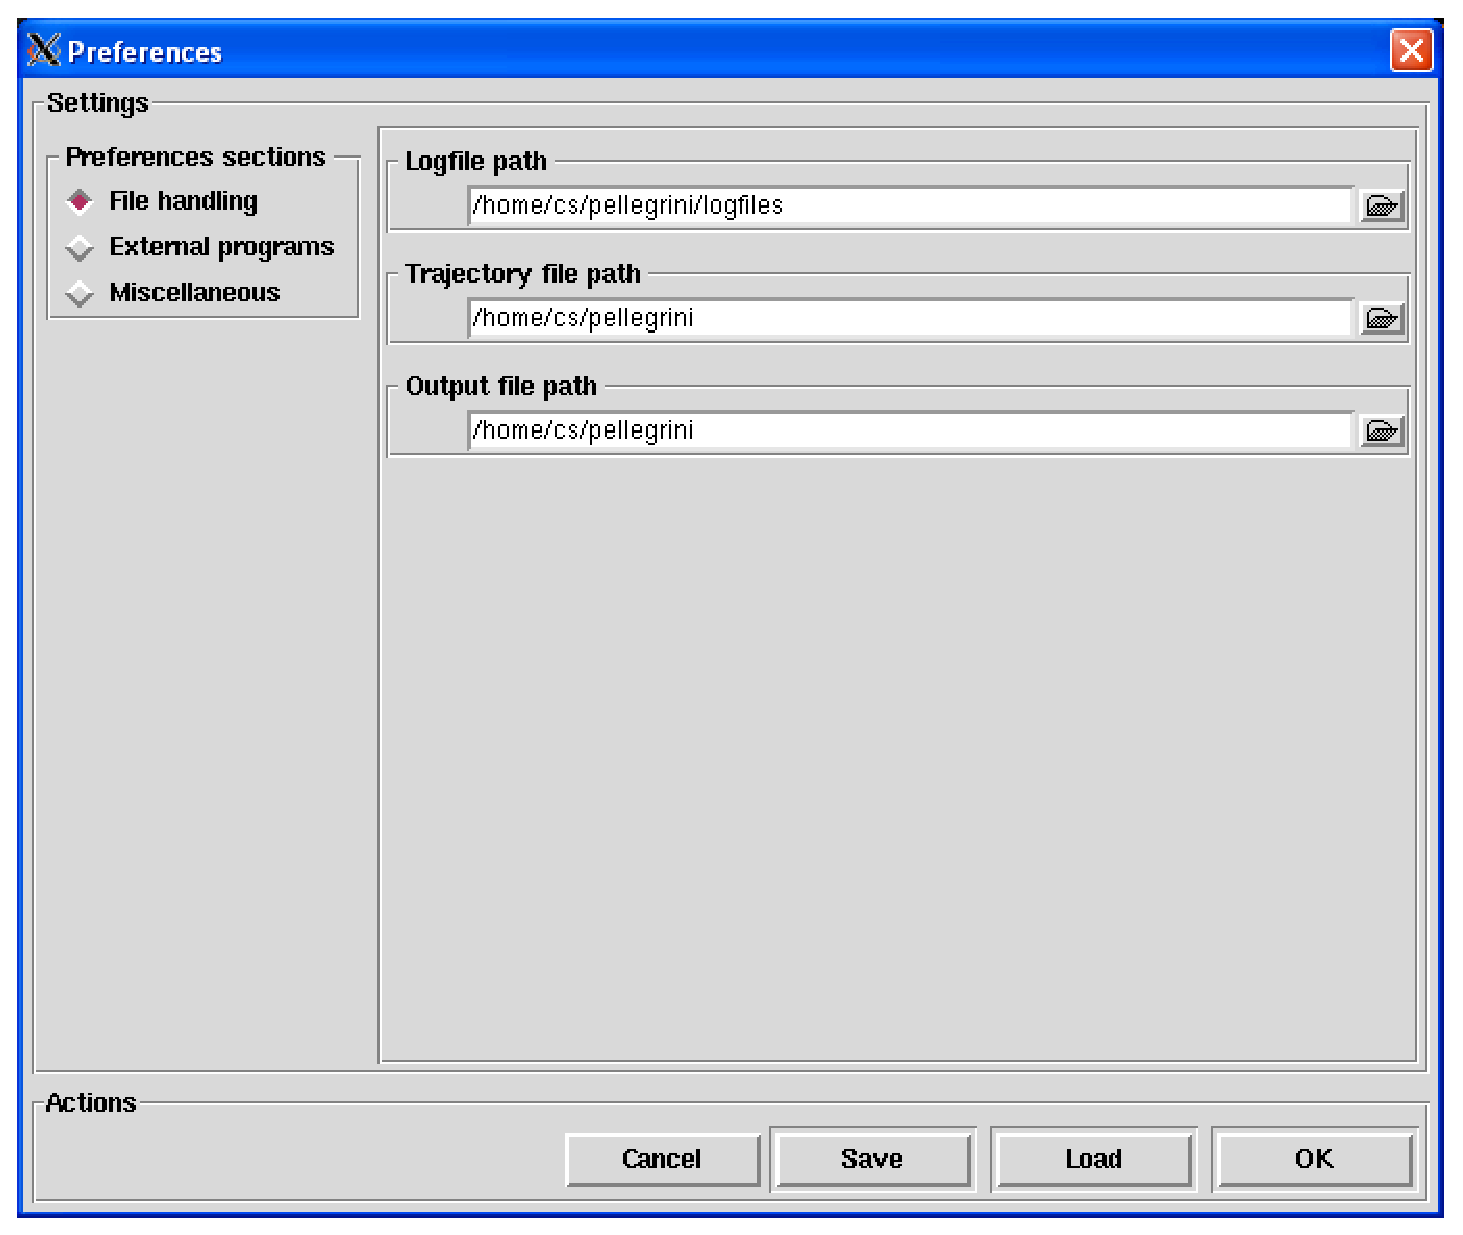
\includegraphics[width=5.2cm]{Figures/preferences_file_handling.eps}
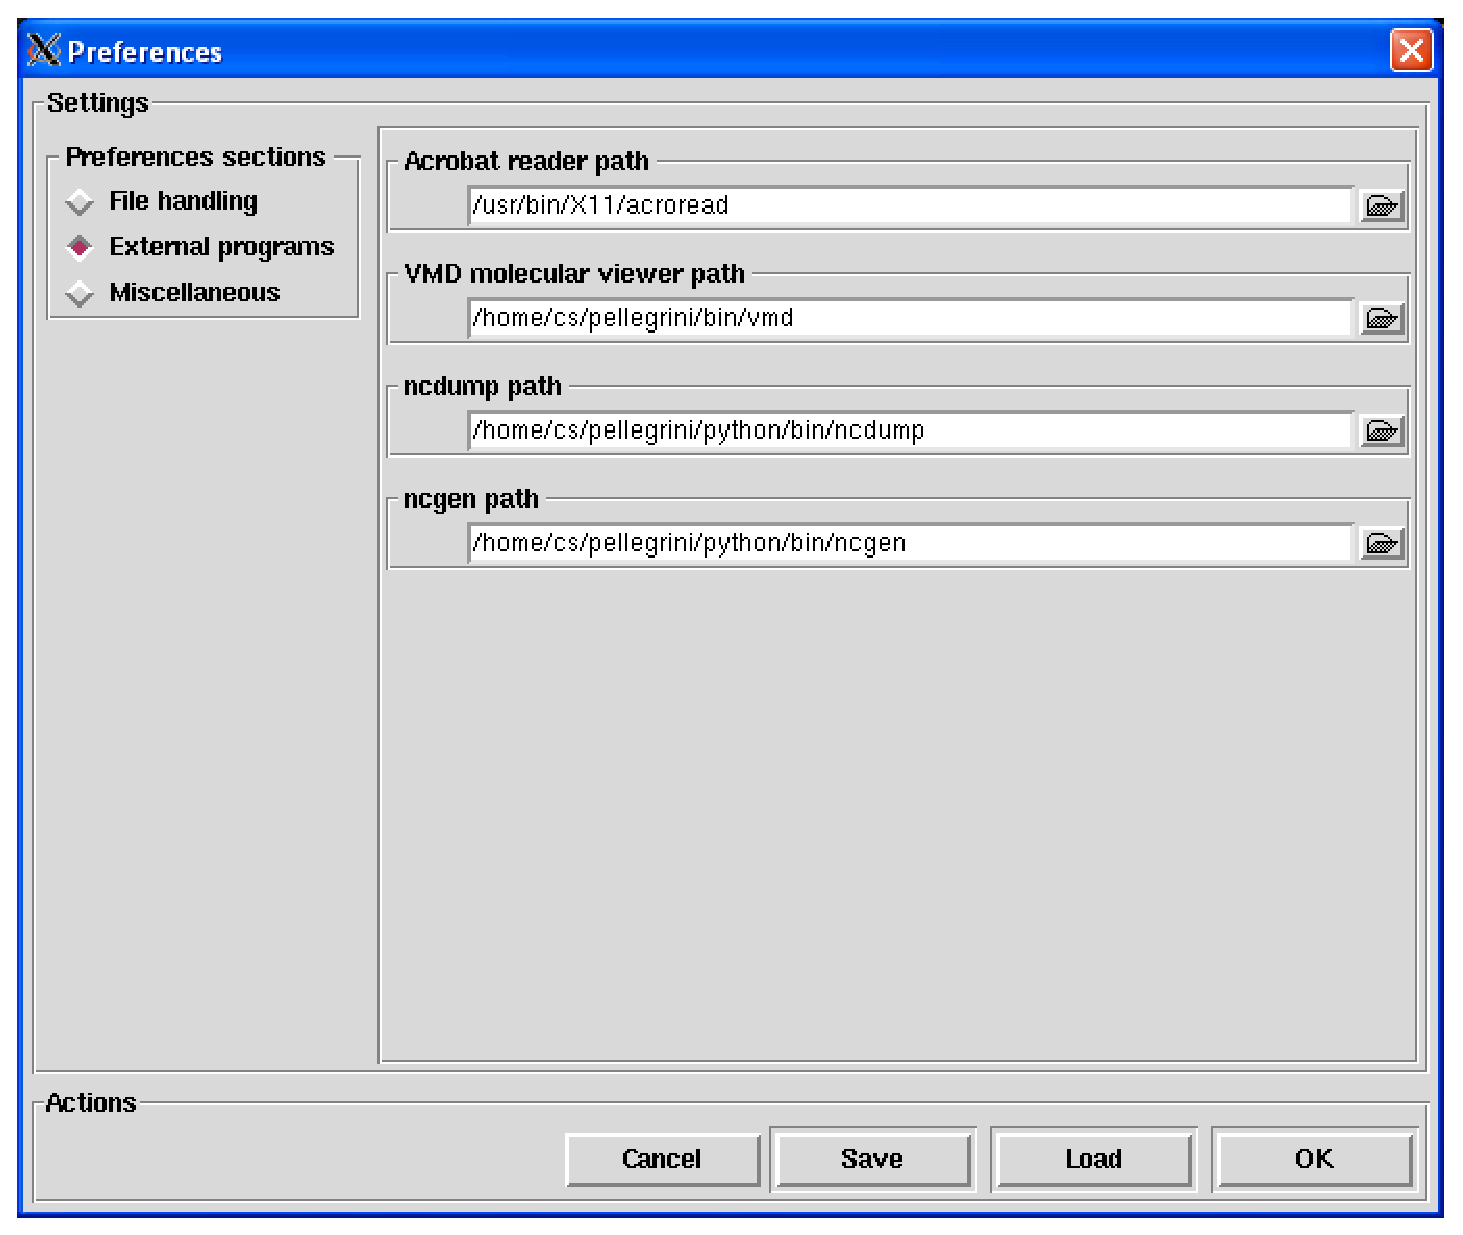
\includegraphics[width=5.2cm]{Figures/preferences_external_programs.eps}
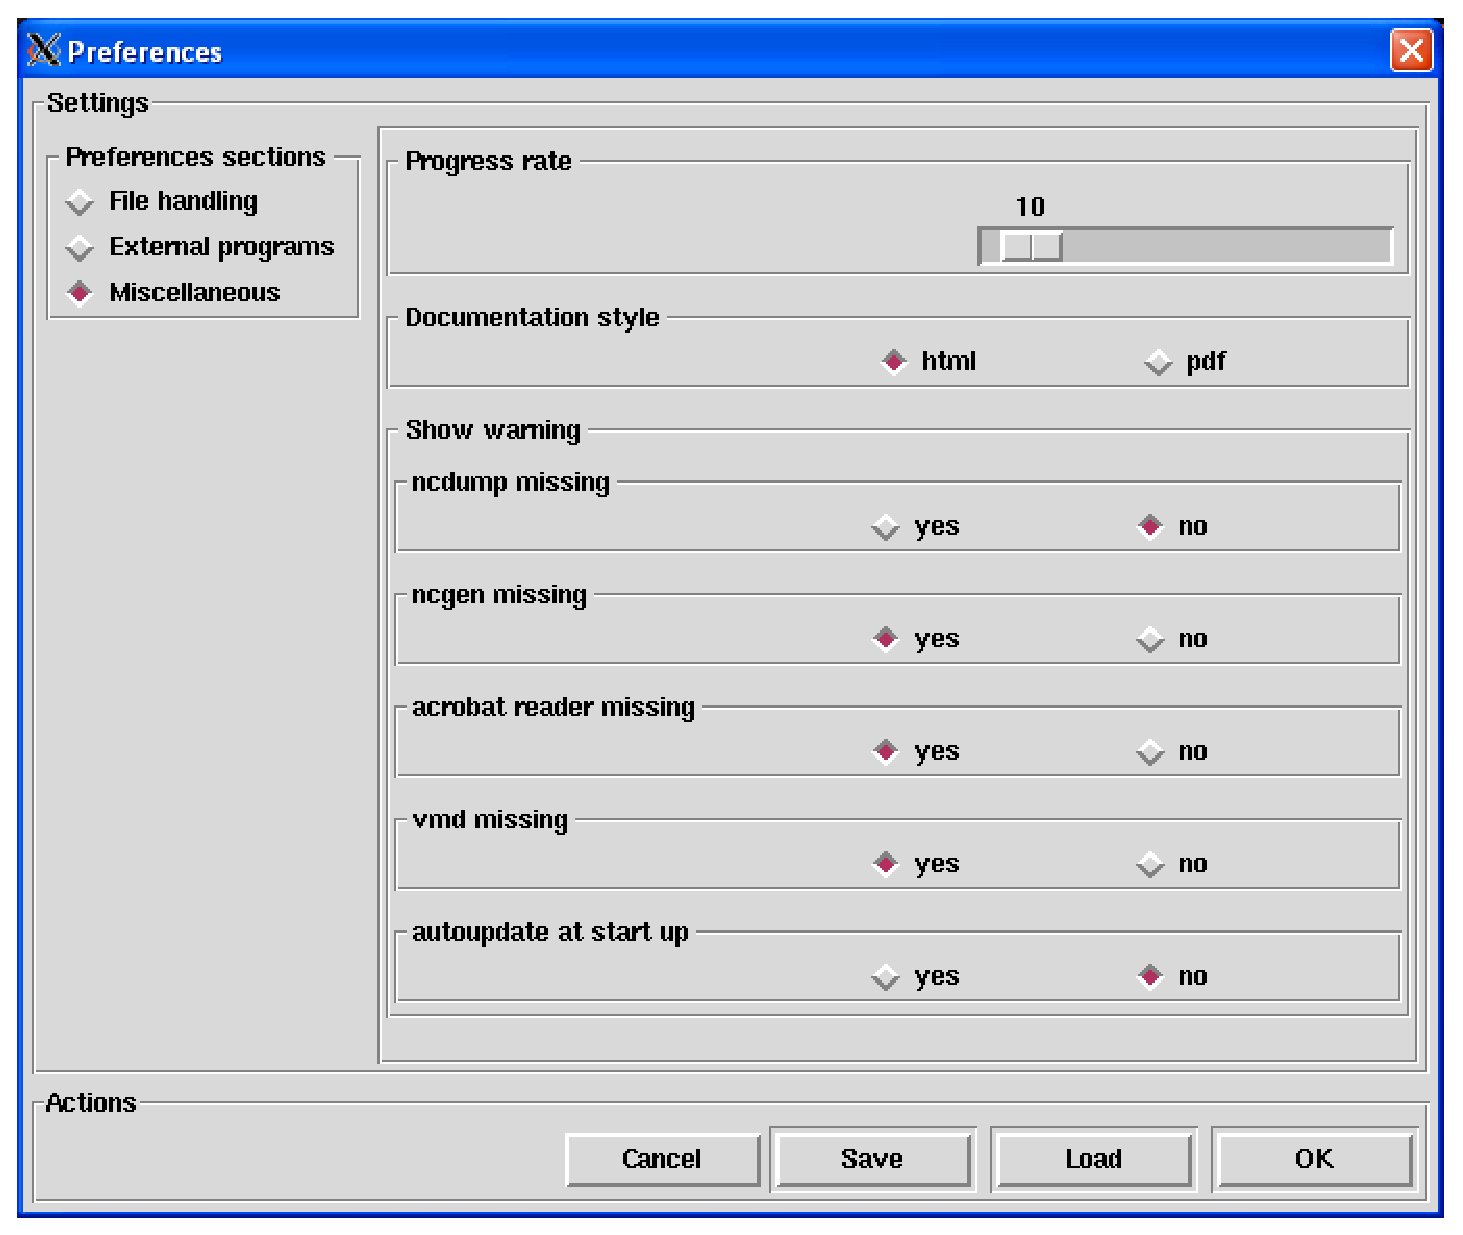
\includegraphics[width=5.2cm]{Figures/preferences_miscellaneous.eps}
\end{center}
\caption[The three preferences sections]{The three preferences sections dialogs available in \NMOLDYN . On the left, 
the \textbf{file handling} section, on the middle the \textbf{external programs} section and on the right, the \textbf{miscellaneous} section.}
\label{fig:preferences_sections}
\end{figure}   
\newpage
Each preference section dialog contains an entry for each of its associated preferences variable initialized with a 
default value. Here is the list of the \NMOLDYN\ preferences variables:
\begin{itemize}
\item \textbf{Logfile path}\\
\textbf{Section:} File handling\\
\textbf{Preferences variable name:} logfile\_path\\
\textbf{Format:} string\\
\textbf{Default:} The user \$HOME directory\\
\textbf{Description:} The path for the directory where the \NMOLDYN\ log files will be written.

\item \textbf{Trajectory file path}\\
\textbf{Section:} File handling\\
\textbf{Preferences variable name:} trajfile\_path\\
\textbf{Format:} string\\
\textbf{Default:} The user \$HOME directory\\
\textbf{Description:} The path for the directory where the \MMTK\ \NetCDF\ trajectories will be loaded by default.

\item \textbf{Output file path}\\
\textbf{Section:} File handling\\
\textbf{Preferences variable name:} outputfile\_path\\
\textbf{Format:} string\\
\textbf{Default:} The user \$HOME directory\\
\textbf{Description:} The path for the directory where the \NMOLDYN\ output files will be written.

\item \textbf{Acrobat reader path}\\
\textbf{Section:} External programs\\
\textbf{Preferences variable name:} acroread\_path\\
\textbf{Format:} string\\
\textbf{Default:} \textit{None}\\
\textbf{Description:} The path for the acrobat reader executable. If this path is not set, it will not be possible to display the 
documentation in pdf format.

\item \textbf{VMD molecular viewer path}\\
\textbf{Section:} External programs\\
\textbf{Preferences variable name:} vmd\_path\\
\textbf{Format:} string\\
\textbf{Default:} \textit{None}\\
\textbf{Description:} The path for the \textbf{VMD} molecular viewer executable \cite{VMD}. If this path is not set, the 
\textbf{Animate} and \textbf{Effective mode} options of the \textbf{View}  menu will be disabled.
\newpage
\item \textbf{ncdump path}\\
\textbf{Section:} External programs\\
\textbf{Preferences variable name:} ncdump\_path\\
\textbf{Format:} string\\
\textbf{Default:} \textit{None}\\
\textbf{Description:} The path for the \textbf{ncdump} executable. If this path is not set, the 
\textbf{Convert NetCDF to ASCII} option of the \textbf{File} menu will be disabled.

\item \textbf{ncgen path}\\
\textbf{Section:} External programs\\
\textbf{Preferences variable name:} ncgen\_path\\
\textbf{Format:} string\\
\textbf{Default:} \textit{None}\\
\textbf{Description:} The path for the \textbf{ncgen} executable. 
If this path is not set, the \textbf{Convert ASCII to NetCDF} option of the \textbf{File} menu will be disabled.

\item \textbf{Progress rate}\\
\textbf{Section:} Miscellaneous\\
\textbf{Preferences variable name:} progress\_rate\\
\textbf{Format:} not an editable entry\\
\textbf{Default:} \textit{10}\\
\textbf{Description:} The rate at which the progress of a \NMOLDYN\ analysis will be displayed on the console and written 
in the \NMOLDYN\ log file.

\item \textbf{Documentation style}\\
\textbf{Section:} Miscellaneous\\
\textbf{Preferences variable name:} documentation\_style\\
\textbf{Format:} not an editable entry\\
\textbf{Default:} \textit{html}\\
\textbf{Description:} The format for the \NMOLDYN\ users guide when clicking on \textit{Help --$>$ Help} item and for the 
online help. HTML if \textbf{html} is selected, PDF if \textbf{pdf} is selected.

\item \textbf{ncdump missing}\\
\textbf{Section:} Miscellaneous\\
\textbf{Preferences variable name:} warning\_ncdump\\
\textbf{Format:} no an editable entry\\
\textbf{Default:} \textit{yes}\\
\textbf{Description:} If set to \textit{yes}, you will be informed if \textbf{ncdump} was not found at each \NMOLDYN\ start 
and each time the \textbf{Preferences} dialog is closed.

\item \textbf{ncgen missing}\\
\textbf{Section:} Miscellaneous\\
\textbf{Preferences variable name:} warning\_ncgen\\
\textbf{Format:} no an editable entry\\
\textbf{Default:} \textit{yes}\\
\textbf{Description:} If set to \textit{yes}, you will be informed if \textbf{ncgen} was not found at each \NMOLDYN\ start 
and each time the \textbf{Preferences} dialog is closed.

\item \textbf{VMD missing}\\
\textbf{Section:} Miscellaneous\\
\textbf{Preferences variable name:} warning\_vmd\\
\textbf{Format:} no an editable entry\\
\textbf{Default:} \textit{yes}\\
\textbf{Description:} If set to \textit{yes}, you will be informed if \textbf{VMD} was not found at each \NMOLDYN\ start 
and each time the \textbf{Preferences} dialog is closed.

\item \textbf{acrobat reader missing}\\
\textbf{Section:} Miscellaneous\\
\textbf{Preferences variable name:} warning\_acroread\\
\textbf{Format:} no an editable entry\\
\textbf{Default:} \textit{yes}\\
\textbf{Description:} If set to \textit{yes}, you will be informed if \textbf{acrobat reader} was not found at each \NMOLDYN\ start 
and each time the \textbf{Preferences} dialog is closed.
\end{itemize}

The \textbf{Actions} frame contains four buttons which are respectively:
\begin{itemize}
\item \textbf{Cancel}
\item \textbf{Save}
\item \textbf{Load}
\item \textbf{OK}
\end{itemize} 
Pressing the \textbf{Cancel} button will cancel the preferences settings and close the preferences dialog leaving the preferences in the state they
were when opening the \textbf{Preferences} dialog. 
Pressing the \textbf{Save} button will pop up a file browser from which you will select a location to save the preferences. 
By default, the preferences file name is:
\\\\
{\ttfamily \$USERPROFILE\textbackslash Application Data\textbackslash nMOLDYN\textbackslash nMOLDYN.ini} on Windows,
\\\\
{\ttfamily \$HOME/.nMOLDYN} on Unix and,
\\\\
{\ttfamily \$HOME/Library/Preferences/nMOLDYN.pref} on MacOS
\\\\
If those paths does not exist, they will be created. These default paths will be the ones that will be searched 
when \NMOLDYN\ is started. Pressing the \textbf{Load} button will load a preferences file through a dialog. \textbf{OK} will
use the settings for the running session of \NMOLDYN\ but will not save them.

The figure \ref{fig:preferences_config_file_example} shows an example of a \NMOLDYN\ preferences file built under a linux 
workstation. Please note the format that must be strictly respected.
\newpage
\begin{figure}[h!]
\begin{center}
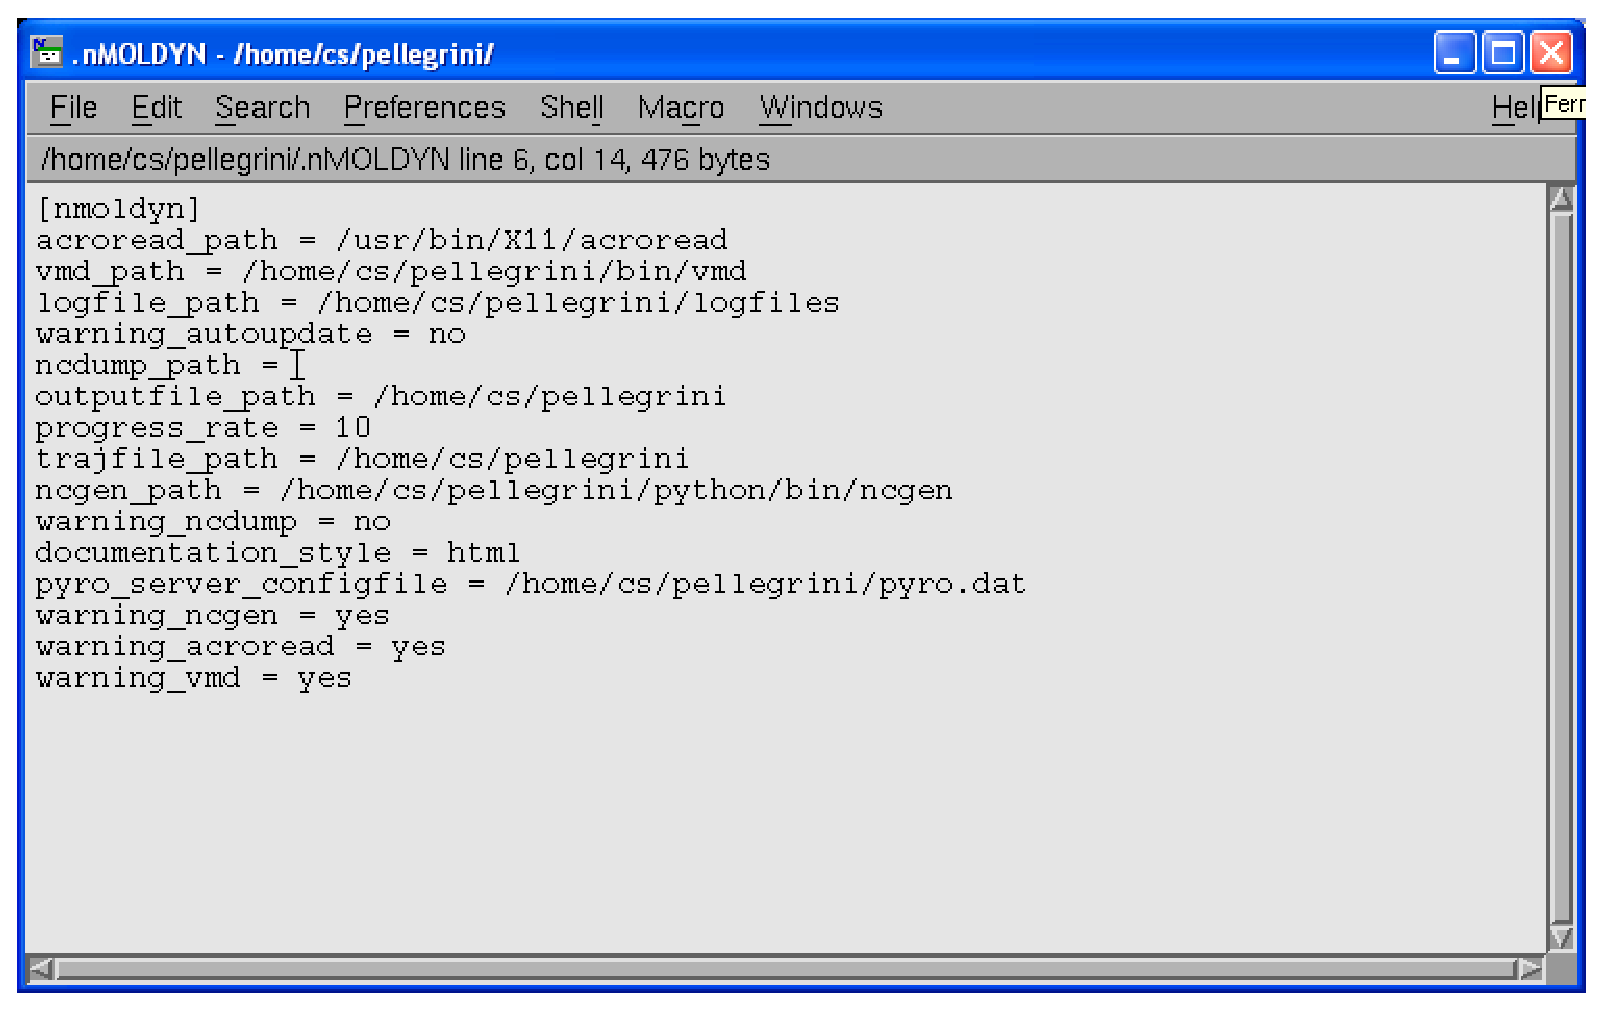
\includegraphics[width=10cm]{Figures/preferences_config_file_example.eps}
\end{center}
\caption[Example of a preferences file]{Example of a \NMOLDYN\ preferences file.}
\label{fig:preferences_config_file_example}
\end{figure}   

As can be seen from that figure, the file must start with the line '[nmoldyn]' followed by th declaration of each preferences 
variables. For the vairables that may be missing in that file or with an empty value (e.g. ncdump\_path in figure 
\ref{fig:preferences_config_file_example}), the default value will be used.

\subsection{Quit}
\label{quit}
Pressing the \textbf{Quit} menubutton will close \NMOLDYN .

\section{The \textbf{Analysis} menu}
\label{analysis_menu}
Pressing the \textbf{Analysis} menubutton brings up a menu from which it is possible to choose the following menus:
\begin{itemize}
\item Dynamics
\item Scattering
\item Structure
\item NMR
\end{itemize}

In this section we will review each of these menus. However, we will first introduce three concepts that are common 
to almost all the analysis available in \NMOLDYN\ which are:
\begin{itemize}
\item weighting scheme
\item atom selection
\item \NMOLDYN\ running modes
\end{itemize}
\newpage
\subsection{Weighting scheme}
\label{weighting_scheme}
In quantities that are averages over all atoms, \NMOLDYN\ gives the possibility to choose between differents atomic weighting 
schemes. Presently, \NMOLDYN\ implements the following schemes:

\begin{itemize}
\item Equal weighting:
\begin{equation}
\label{eq:equal}
\omega_{\alpha}=\frac{1}{N_{atoms}}
\end{equation}
\item Mass weighting: 
\begin{equation}
\label{eq:mass}
\omega_{\alpha}=\frac{m_\alpha}{\sum_{\alpha=1}^{N_{atoms}} m_\alpha}
\end{equation}
\item Atomic number weighting: 
\begin{equation}
\label{eq:atomic_number}
\omega_{\alpha}=\frac{Z_\alpha}{\sum_{\alpha=1}^{N_{atoms}} Z_\alpha}
\end{equation}
\item Incoherent neutron scattering: 
\begin{equation}
\label{eq:incoherent}
\omega_{\alpha}=\frac{b_{\alpha,\mathrm{inc}}^2}{\sum_{\alpha=1}^{N_{atoms}} b_{\alpha,\mathrm{inc}}^2}
\end{equation}
\item Coherent neutron scattering: 
\begin{equation}
\label{eq:coherent}
\sqrt{\omega_{\alpha}}=\frac{b_{\alpha,\mathrm{coh}}}{\sqrt{\sum_{\alpha=1}^{N_{atoms}} b_{\alpha,\mathrm{coh}}^2}}
\end{equation}
\end{itemize}

where $\omega_\alpha$ is the weight for atom $\alpha$, $N_{atoms}$ is the number of (selected) atoms in the system (or in 
the subsystem) for which the analysis is performed and $m_\alpha$, $Z_\alpha$, $b_{\alpha,\mathrm{inc}}$, and $b_{\alpha,\mathrm{coh}}$ are respectively the 
mass, the atomic number, the incoherent scattering length and the coherent scattering length of atom $\alpha$ where

\begin{eqnarray}
b_{\alpha,\mathrm{coh}}&=&\overline{b_\alpha} \\
b_{\alpha,\mathrm{inc}}&=&\sqrt{\overline{b_\alpha^2}-\overline{b_\alpha}^2}
\end{eqnarray} 

the average being done over isotopes and relative spin orientations of neutrons and nucleus. 

Using such a definition, we have $\sum_{\alpha=1}^N \omega_\alpha=1$.

If we now group atoms into their different species \textit{A}, \textit{B} \ldots (e.g. oxygens, hydrogens \ldots ) such that:
\begin{equation}
N = \sum^{N_{species}}_{I = 1}n_I
\end{equation}

where $N_{species}$ is the total number of selected species and $n_I$ is the number of atoms of specie \textit{I}. Then, we can 
define the weight for a given atomic specie \textit{I} as:

\begin{itemize}
\item Equal weighting (per specie):
\begin{equation}
\label{eq:equal_specie}
{\cal W_I}=\frac{n_I}{N_{atoms}}
\end{equation}
\item Mass weighting (per specie): 
\begin{equation}
\label{eq:mass_specie}
{\cal W_I}=\frac{n_{I}m_{I}}{\sum^{N_{species}}_{I=1} n_{I}m_{I}}
\end{equation}
\item Atomic number weighting: 
\begin{equation}
\label{eq:atomic_number_specie}
{\cal W_I}=\frac{n_{I}Z_{I}}{\sum^{N_{species}}_{I=1} n_{I}Z_{I}}
\end{equation}
\item Incoherent neutron scattering: 
\begin{equation}
\label{eq:incoherent_specie}
{\cal W_I}=\frac{n_{I}b_{I,\mathrm{inc}}^2}{\sum^{N_{species}}_{I=1} b_{I,\mathrm{inc}}^2}
\end{equation}
\item Coherent neutron scattering: 
\begin{equation}
\label{eq:coherent_specie}
\sqrt{{\cal W_I}}=\frac{n_{I}b_{I,\mathrm{coh}}}{\sqrt{\sum^{N_{species}}_{I=1} b_{I,\mathrm{coh}}^2}}
\end{equation}
\end{itemize}
and we have $\sum_{I=1}^{N_{species}} {\cal W_I}=\sum_{I=1}^{N_{species}}\sum_{\alpha=1}^{n_I} \omega_{\alpha,I}= 1$ where 
$\omega_{\alpha,I}$ is the atomic weight of atom $\alpha$ of specie $I$ defined in equations 
\ref{eq:equal} to \ref{eq:mass}. The weigthing scheme based on specie will be useful when dealing with analysis for which 
partial terms can be defined.

\subsection{Atom selection}
\label{atom_selection}
It is sometimes necessary to define a subset of atoms on which a given action or analysis will be performed.
\NMOLDYN\ provided this possibility by a general mechanism that can be applied to several selection types such 
as:
\begin{itemize}
\item Subset selection: selection of a subset of atoms on which an analysis will be performed,
\item Deuteration selection: definition of a subset of hydrogen atoms whose parameters will be the ones of deuterium. This allows 
to account for isotopic deuteration replacement performed in neutron experiments,
\item Group selection: definition of one or several groups of atoms on which a given action will be performed collectively.
\end{itemize}
Albeit different in their nature, we will see in the following sections, that all these selections use the same syntax 
what is quite convenient from a user point of view.

\subsubsection{Subset selection}
\label{subset_selection}
This kind of selection is used when one wants to narrow an analysis on a given subset of atoms of the 
system. For instance, assuming that you performed a \MD\ of a protein in a water box and that 
you are interested in calculating the diffusion constant of the protein via a \MSD\ analysis. In that case, 
it will be necessary to perform the analysis only on the atoms of the protein. 
\newpage
By default, \NMOLDYN\ consider all the atoms for an analysis. The dialog from which a subset selection is performed 
is displayed in figure \ref{fig:subset_selection}.
\begin{figure}[h!]
\begin{center}
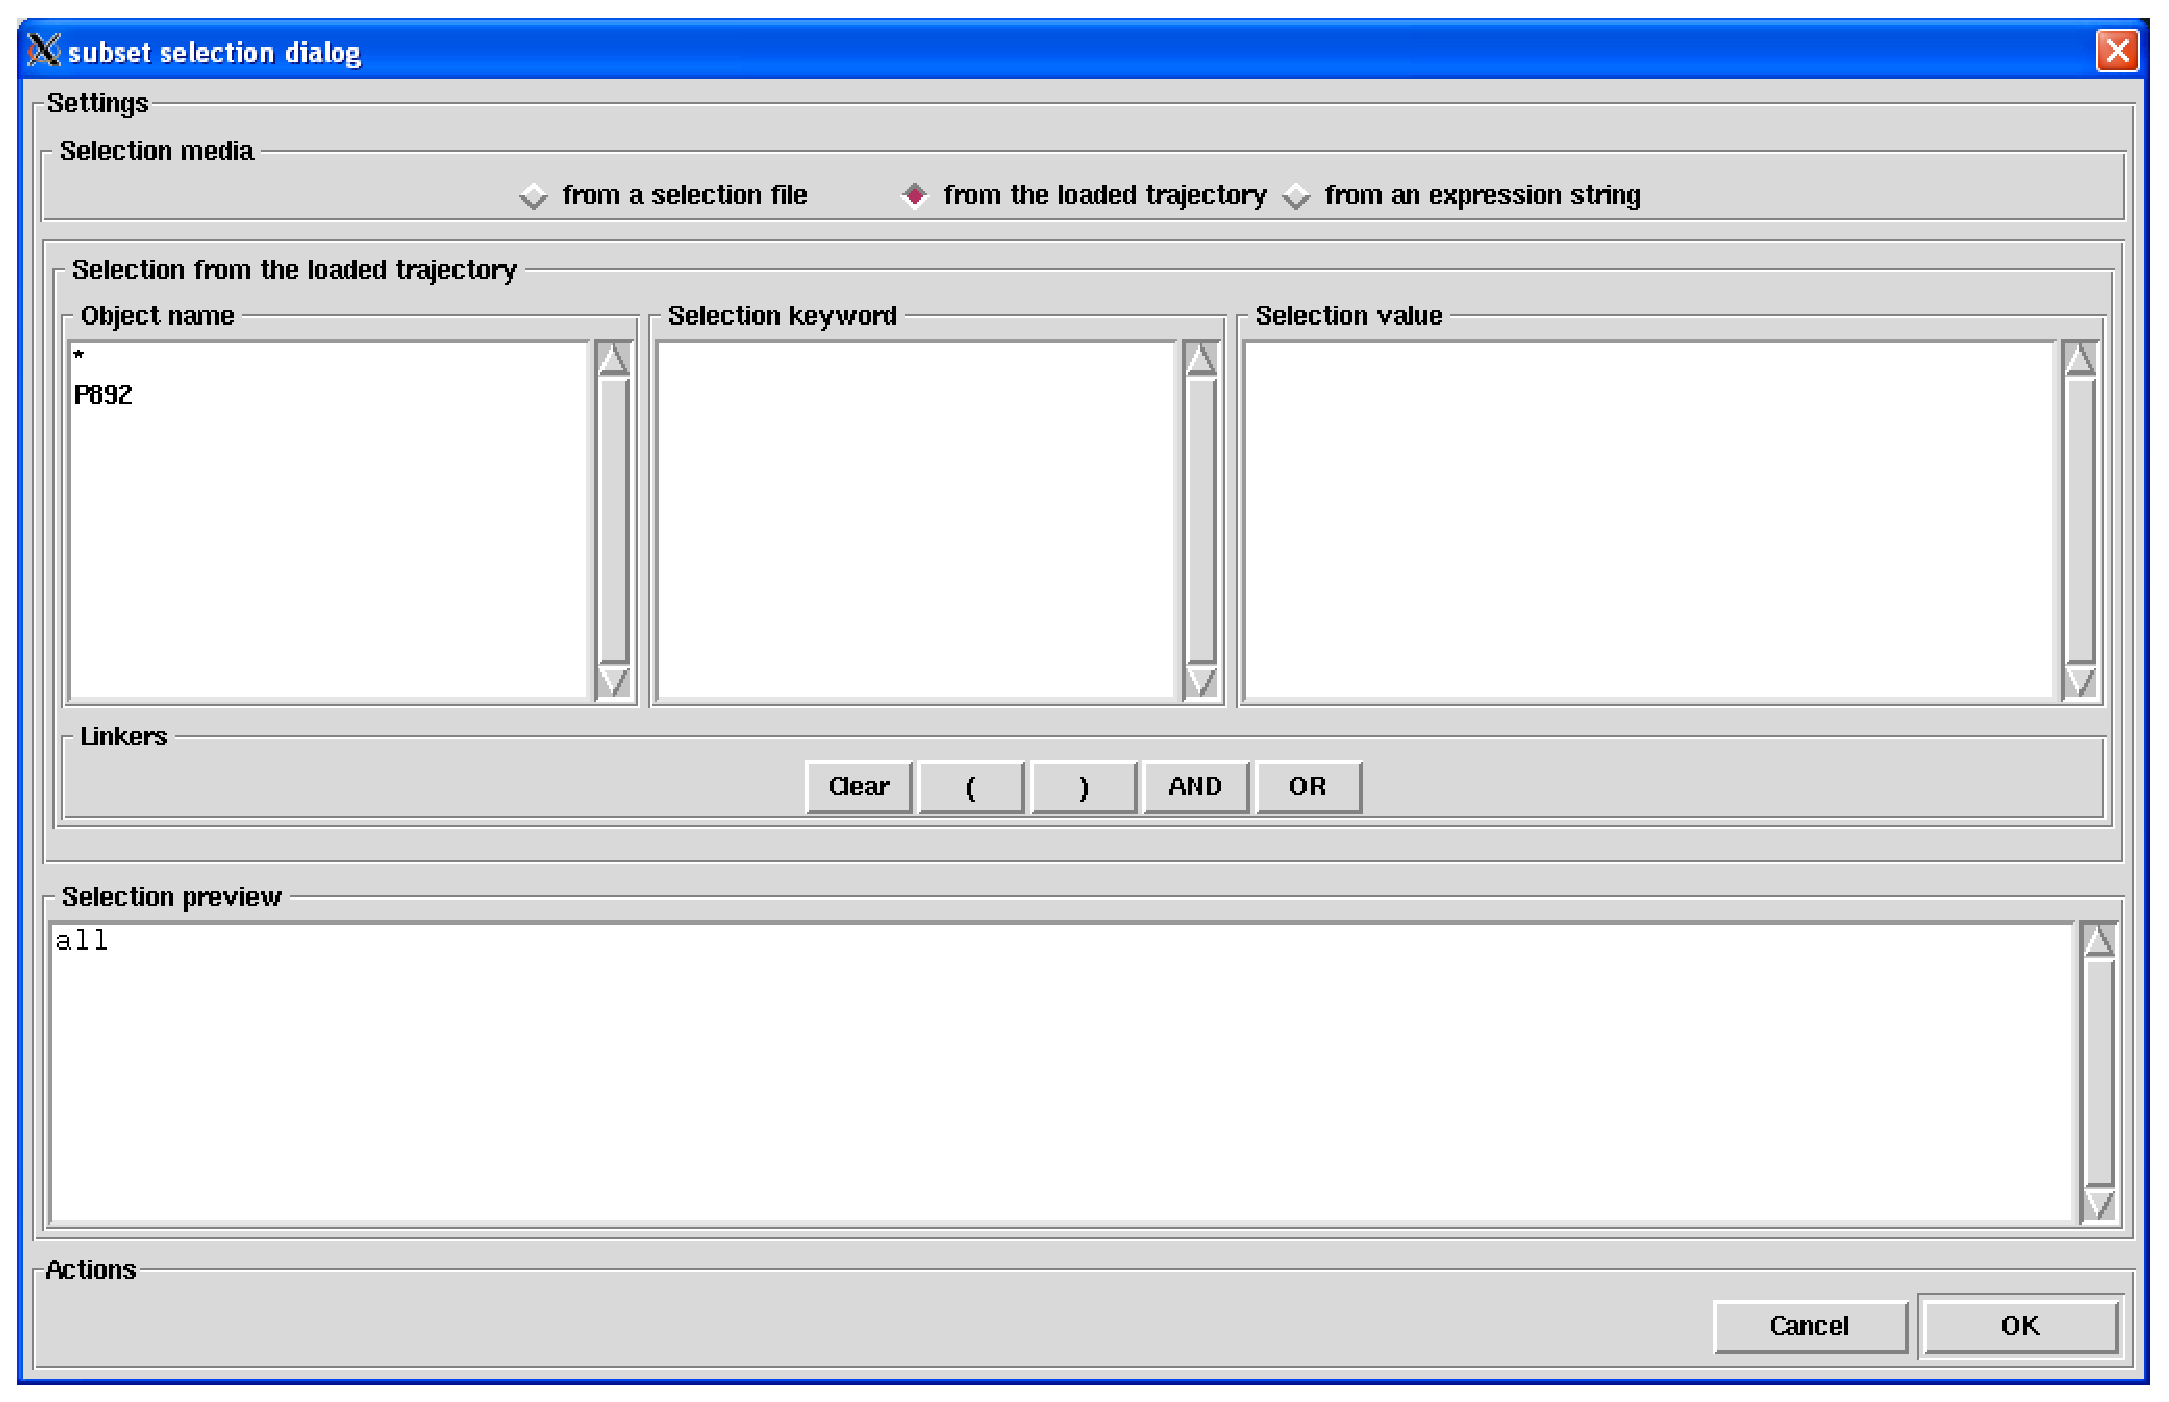
\includegraphics[width=10cm]{Figures/subset_selection.eps}
\end{center}
\caption[The subset selection dialog]{The dialog from where a subset selection is performed.}
\label{fig:subset_selection}
\end{figure}   

At the bottom of the dialog, the \textbf{Actions} frame contains the \textbf{Cancel} button to cancel the selection and 
the \textbf{OK} button to validate the selecton.

On the top of the dialog, three radiobuttons allows to select from which media the selection will be performed. This can 
be:
\begin{itemize}
\item \textbf{from a selection file}: this will perform the selection from a \NMOLDYN\ subset selection file,
\item \textbf{from the loaded trajectory}: this will perform the selection directly from the contents of the universe contained 
in the loaded trajectory,
\item \textbf{from an expression string}: this will perform the selection from a valid python expression declaring a list 
of  atoms to include in the selection.
\end{itemize}
When clicking on one of these radiobutton, a media-specific dialog will be displayed in the underneath frame.

\paragraph{selection from a selection file\\}
\label{subset_selection_from_a_selection_file}
To perform a subset selection from a selection file, you have to click on the \textbf{from a selection file} radiobutton. 
A dialog will be displayed in the underneath frame from which you will be asked for a subset selection file 
(see Fig. \ref{fig:subset_selection_from_a_selection_file}).
\newpage
\begin{figure}[h!]
\begin{center}
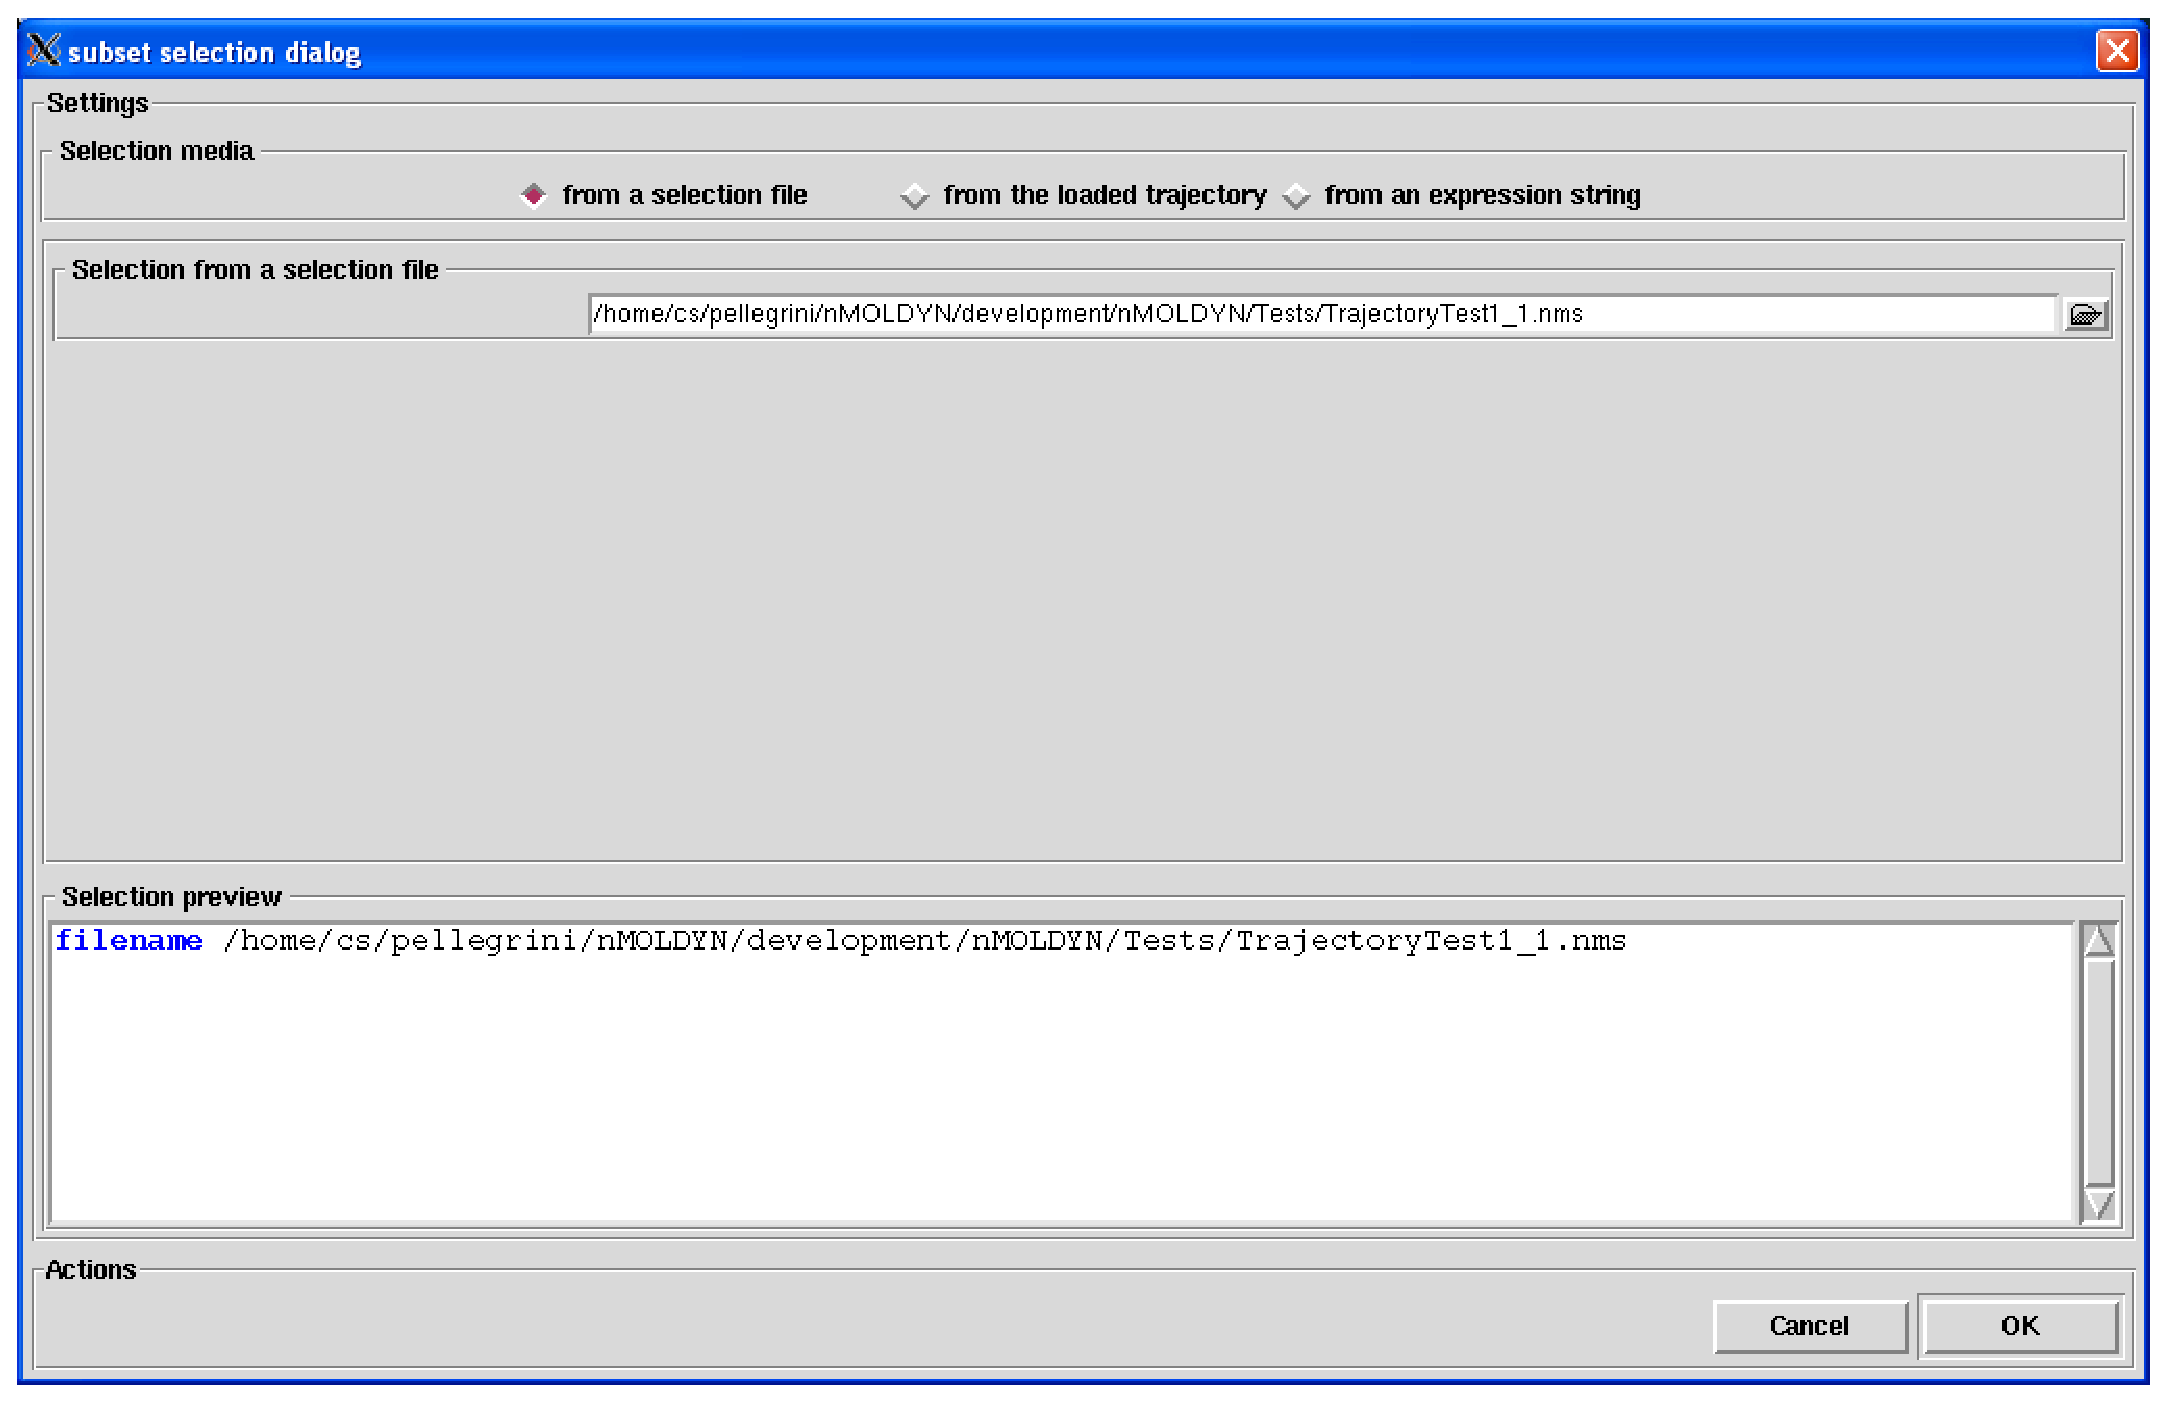
\includegraphics[width=10cm]{Figures/subset_selection_from_a_selection_file.eps}
\end{center}
\caption[The subset selection dialog for a selection from a selection file]{The subset selection dialog for a selection from a selection file.}
\label{fig:subset_selection_from_a_selection_file}
\end{figure}   

The format of a \NMOLDYN\ selection file is quite simple. It is an ASCII file with the \textbf{.nms} extension whose contents is a 
python script made of two lines. The first line must set the variable \textit{pdb} to the path of a \PDB\ file of the first frame of the trajectory being 
processed (it can be obtained using the frame extractor tool described in section \ref{frame_snapshot} for example).The second 
line must set the variable \textit{subset} to a list of integers where each integers represents the \PDB\ serial number of the atoms 
to select. An example of a subset selection file is shown in figure \ref{fig:subset_selection_file}.
\begin{figure}[h!]
\begin{center}
\includegraphics[width=10cm]{Figures/subset_selection_file.eps}
\end{center}
\caption[Example of a subset selection file]{Example of a subset file.}
\label{fig:subset_selection_file}
\end{figure}   

Once a selection file has been loaded, the constructed selection string that will be used by \NMOLDYN\ for this kind of selection is 
displayed in the \textbf{Selection preview} entry at the bottom of the dialog with highlighted keywords.

\paragraph{selection from the loaded trajectory\\}
To perform a subset selection from the loaded trajectory, you have to click on the \textbf{from the loaded trajectory} radiobutton.
A dialog will be displayed in the underneath frame from which you will construct your selection directly from the contents of the 
universe related to the loaded trajectory (see Fig. \ref{fig:subset_selection_from_the_loaded_trajectory}).
\begin{figure}[h!]
\begin{center}
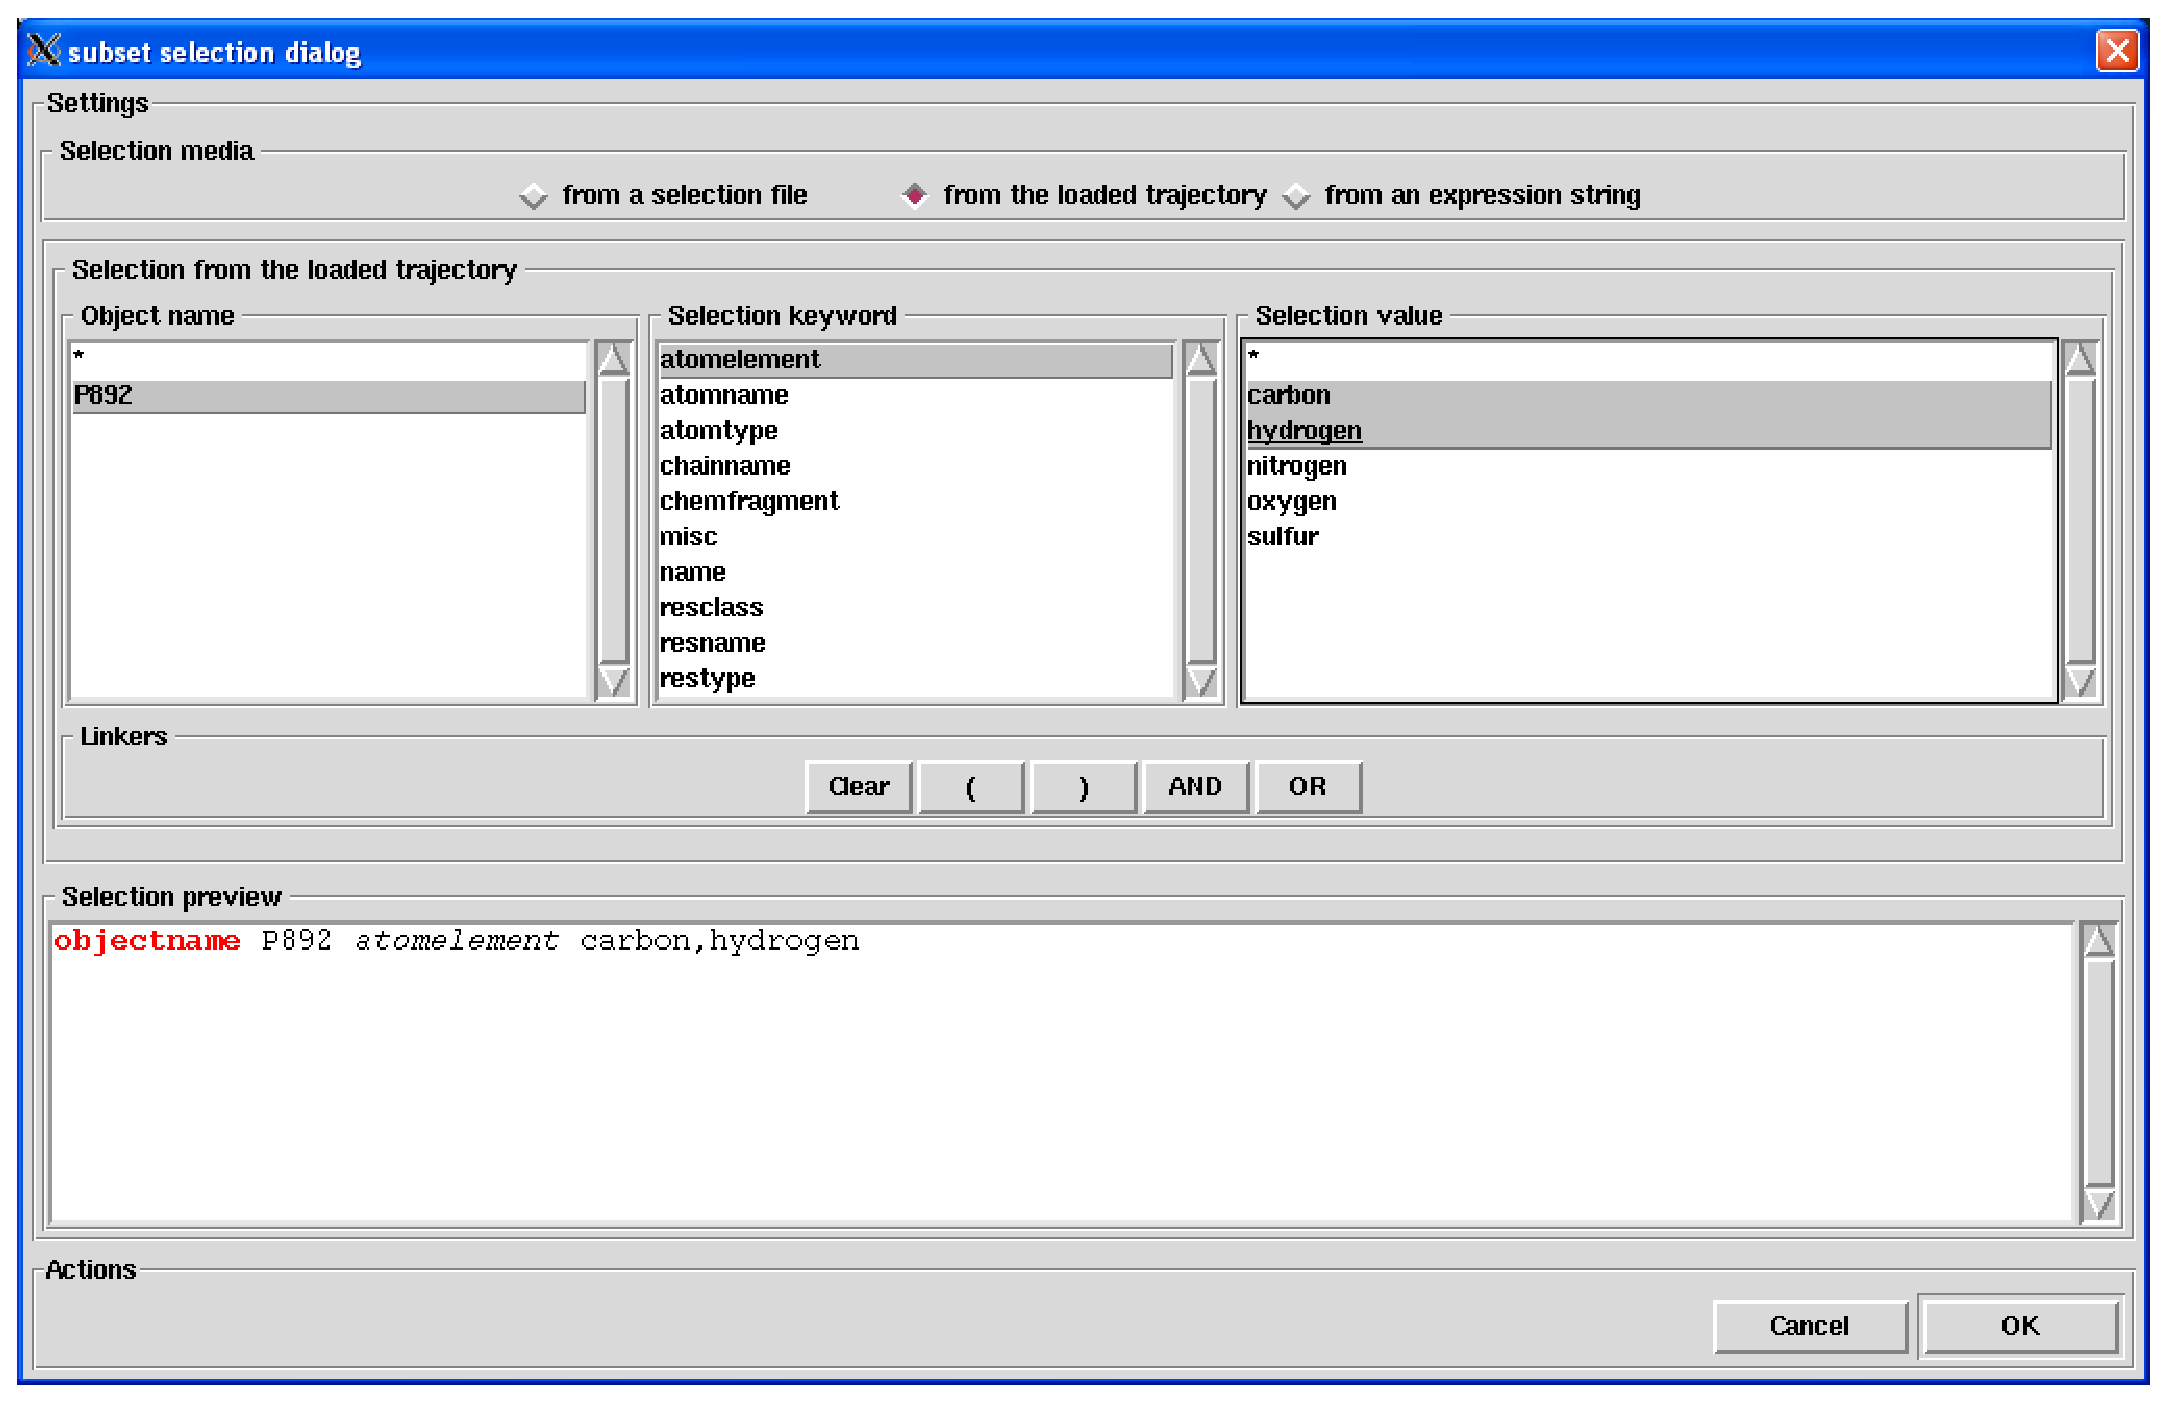
\includegraphics[width=10cm]{Figures/subset_selection_from_the_loaded_trajectory.eps}
\end{center}
\caption[The subset selection dialog for a selection from the loaded trajectory]{The subset selection dialog for a selection from the loaded trajectory.}
\label{fig:subset_selection_from_the_loaded_trajectory}
\end{figure}   

To construct the selection, it is compulsory to proceed in the following order:
\begin{enumerate}
\item select an object name among the ones displayed in the \textbf{Object name} listbox. This will 
display in the \textbf{Selection keywords} listbox the selection keywords associated to the selected object.
\item select a selection keyword among the ones displayed in \textbf{Selection keywords} listbox. This will display in the 
\textbf{Selection value} listbox the values associated to the selected keyword.
\item unselect/select one or several values among the ones displayed in the \textbf{Selection value} listbox.
\end{enumerate}
By doing so, you will construct a selection string with the following format:
\\\\
\textit{objectname name keyword value1,value2, \ldots}
\\\\
where \textit{name} is the selected object name (step 1), \textit{keyword} is the selected keyword (step 2) and 
\textit{value1,value2,\ldots} are the selected values (step 3). This constructed selection string, that will be used by 
\NMOLDYN , is displayed in the \textbf{Selection preview} entry at the bottom of the dialog with highlighted keywords. 

You can associate several selection keywords to a given selected object by repeating steps 2,3. In that case, 
the constructed selection string will have the following format:
\\\\
\textit{objectname name keyword1 value1,value2,\ldots OR keyword2, value1,value2,value3\ldots}
\\\\
where the keyword \textit{OR} will be interpreted by \NMOLDYN\ as an union operator in the sense that it will take the 
union between the set of atoms generated by \textit{keyword1 value1,value2}, \textit{keyword2 value1,value2,value3} \ldots

You can also include several objects in the selection by repeating steps 1,2,3. In that case, the constructed selection 
string will have the following format:
\\\\
\textit{objectname name1 keyword1 value1,\ldots OR keyword2, value1,value2, \ldots OR objectname name2 keyword1 value1 \ldots}
\\\\
Finally, using the buttons within the \textbf{Linkers} frame each time a step 3 is completed allows to construct more complex selection strings using the 
\textbf{(}, \textbf{)}, \textbf{AND}, \textbf{OR} linkers, the \textbf{AND} linker acting as an intersection operator while the 
\textbf{OR} link, described above, acts as an union operator. The button \textbf{Clear} clears up the selection string under construction.

The table \ref{tab:selection_keywords} lists the selection keywords and values depending on the \MMTK\ type of the object being processed.
\begin{table}[h!]
    \begin{small}
    \centering
    \begin{tabular}{|l|c|p{8cm}|}
    \hline
    Object \MMTK\ type & Selection keyword & Selection value \\
    \hline
    Atom            & name        & the object \MMTK\ name\\
    \hline
    AtomCluster     & atomelement & the element name (e.g. hydrogen)\\
    \cline{2-3}
                    & atomname    & the atom \MMTK\ name\\
    \cline{2-3}
                    & name        & the object \MMTK\ name\\
    \hline
    Molecule        & chemfrag    & the chemical fragment name. One of amine, hydroxy, methyl or thiol \\
    \cline{2-3}
                    & atomelement & the element name (e.g. hydrogen)\\
    \cline{2-3}
                    & atomname    & the atom \MMTK\ name\\    
    \hline
    NucleotideChain & atomelement & the element name (e.g. hydrogen)\\
    \cline{2-3}
                    & atomname    & the atom \MMTK\ name\\
    \cline{2-3}
                    & atomtype    & the atom \MMTK\ type\\
    \cline{2-3}
                    & misc        & one of backbone or bases\\
    \cline{2-3}
                    & name        & the object \MMTK\ name\\
    \cline{2-3}
                    & nuclname    & the nucleotide \MMTK\ name.\\
    \cline{2-3}
                    & nucltype    & the nucleotide \MMTK\ type\\
    \hline
    PeptideChain    & chemfrag    & the chemical fragment name. One of amine, c\_alphas, hydroxy, methyl or thiol \\
    \cline{2-3}
                    & atomelement & the element name (e.g. hydrogen)\\
    \cline{2-3}
                    & atomname    & the atom \MMTK\ name\\
    \cline{2-3}
                    & atomtype    & the atom \MMTK\ type\\
    \cline{2-3}
                    & misc        & one of backbone or sidechains\\
    \cline{2-3}
                    & name        & the object \MMTK\ name\\
    \cline{2-3}
                    & resclass    & the residue class. One of acidic, aliphatic, aromatic, basic, charged, hydrophobic, polar or small\\
    \cline{2-3}
                    & resname     & the residue \MMTK\ name\\
    \cline{2-3}
                    & restype     & the residue \MMTK\ type\\
    \hline
    Protein         & chemfrag    & one of amine, c\_alphas, hydroxy, methyl or thiol \\
    \cline{2-3}
                    & atomelement & the element name (e.g. hydrogen)\\
    \cline{2-3}
                    & atomname    & the atom \MMTK\ name\\
    \cline{2-3}
                    & atomtype    & the atom \MMTK\ type\\
    \cline{2-3}
                    & chainname   & the chain \MMTK\ name\\
    \cline{2-3}
                    & misc        & one of backbone or sidechains\\
    \cline{2-3}
                    & name        & the object \MMTK\ name\\
    \cline{2-3}
                    & resclass    & the residue class. One of acidic, aliphatic, aromatic, basic, charged, hydrophobic, polar or small\\
    \cline{2-3}
                    & resname     & the residue \MMTK\ name\\
    \cline{2-3}
                    & restype     & the residue \MMTK\ type\\
    \hline
    \end{tabular}
    \caption[Selection keywords available in \NMOLDYN]{List of selection keywords and their associated values according to the \MMTK\ type of the selected object.}
    \label{tab:selection_keywords}
    \end{small}
\end{table}
\newpage
Here are some examples of subset selection strings constructed from a protein whose name is P892:
\begin{itemize}
\item \textit{objectname P892 atomelement carbon}: will select only the carbon atoms,
\item \textit{objectname P892 atomelement carbon,hydrogen}: will select only the carbon and hydrogen atoms,
\item \textit{objectname P892 atomelement oxygen and restype Ala,Arg}: will select only the oxygen atoms of Alanine and Arginine 
residues,
\item \textit{objectname P892 atomelement carbon OR resclass acidic}: will select all the carbon atoms plus the all the atoms of the acidic residues.
\end{itemize}

\paragraph{selection from an expression string\\}
To perform a subset selection from an expression string, you have to click on the \textbf{from an expression string} 
radiobutton. A dialog will be displayed in the underneath frame from which you will enter a valid Python expression 
that must declare the \textit{selection} variable as a list of atoms of the loaded universe. The variable 
\textit{self.universe} will be used as a reference for that universe (see Fig. \ref{fig:subset_selection_from_an_expression_string}).
\begin{figure}[h!]
\begin{center}
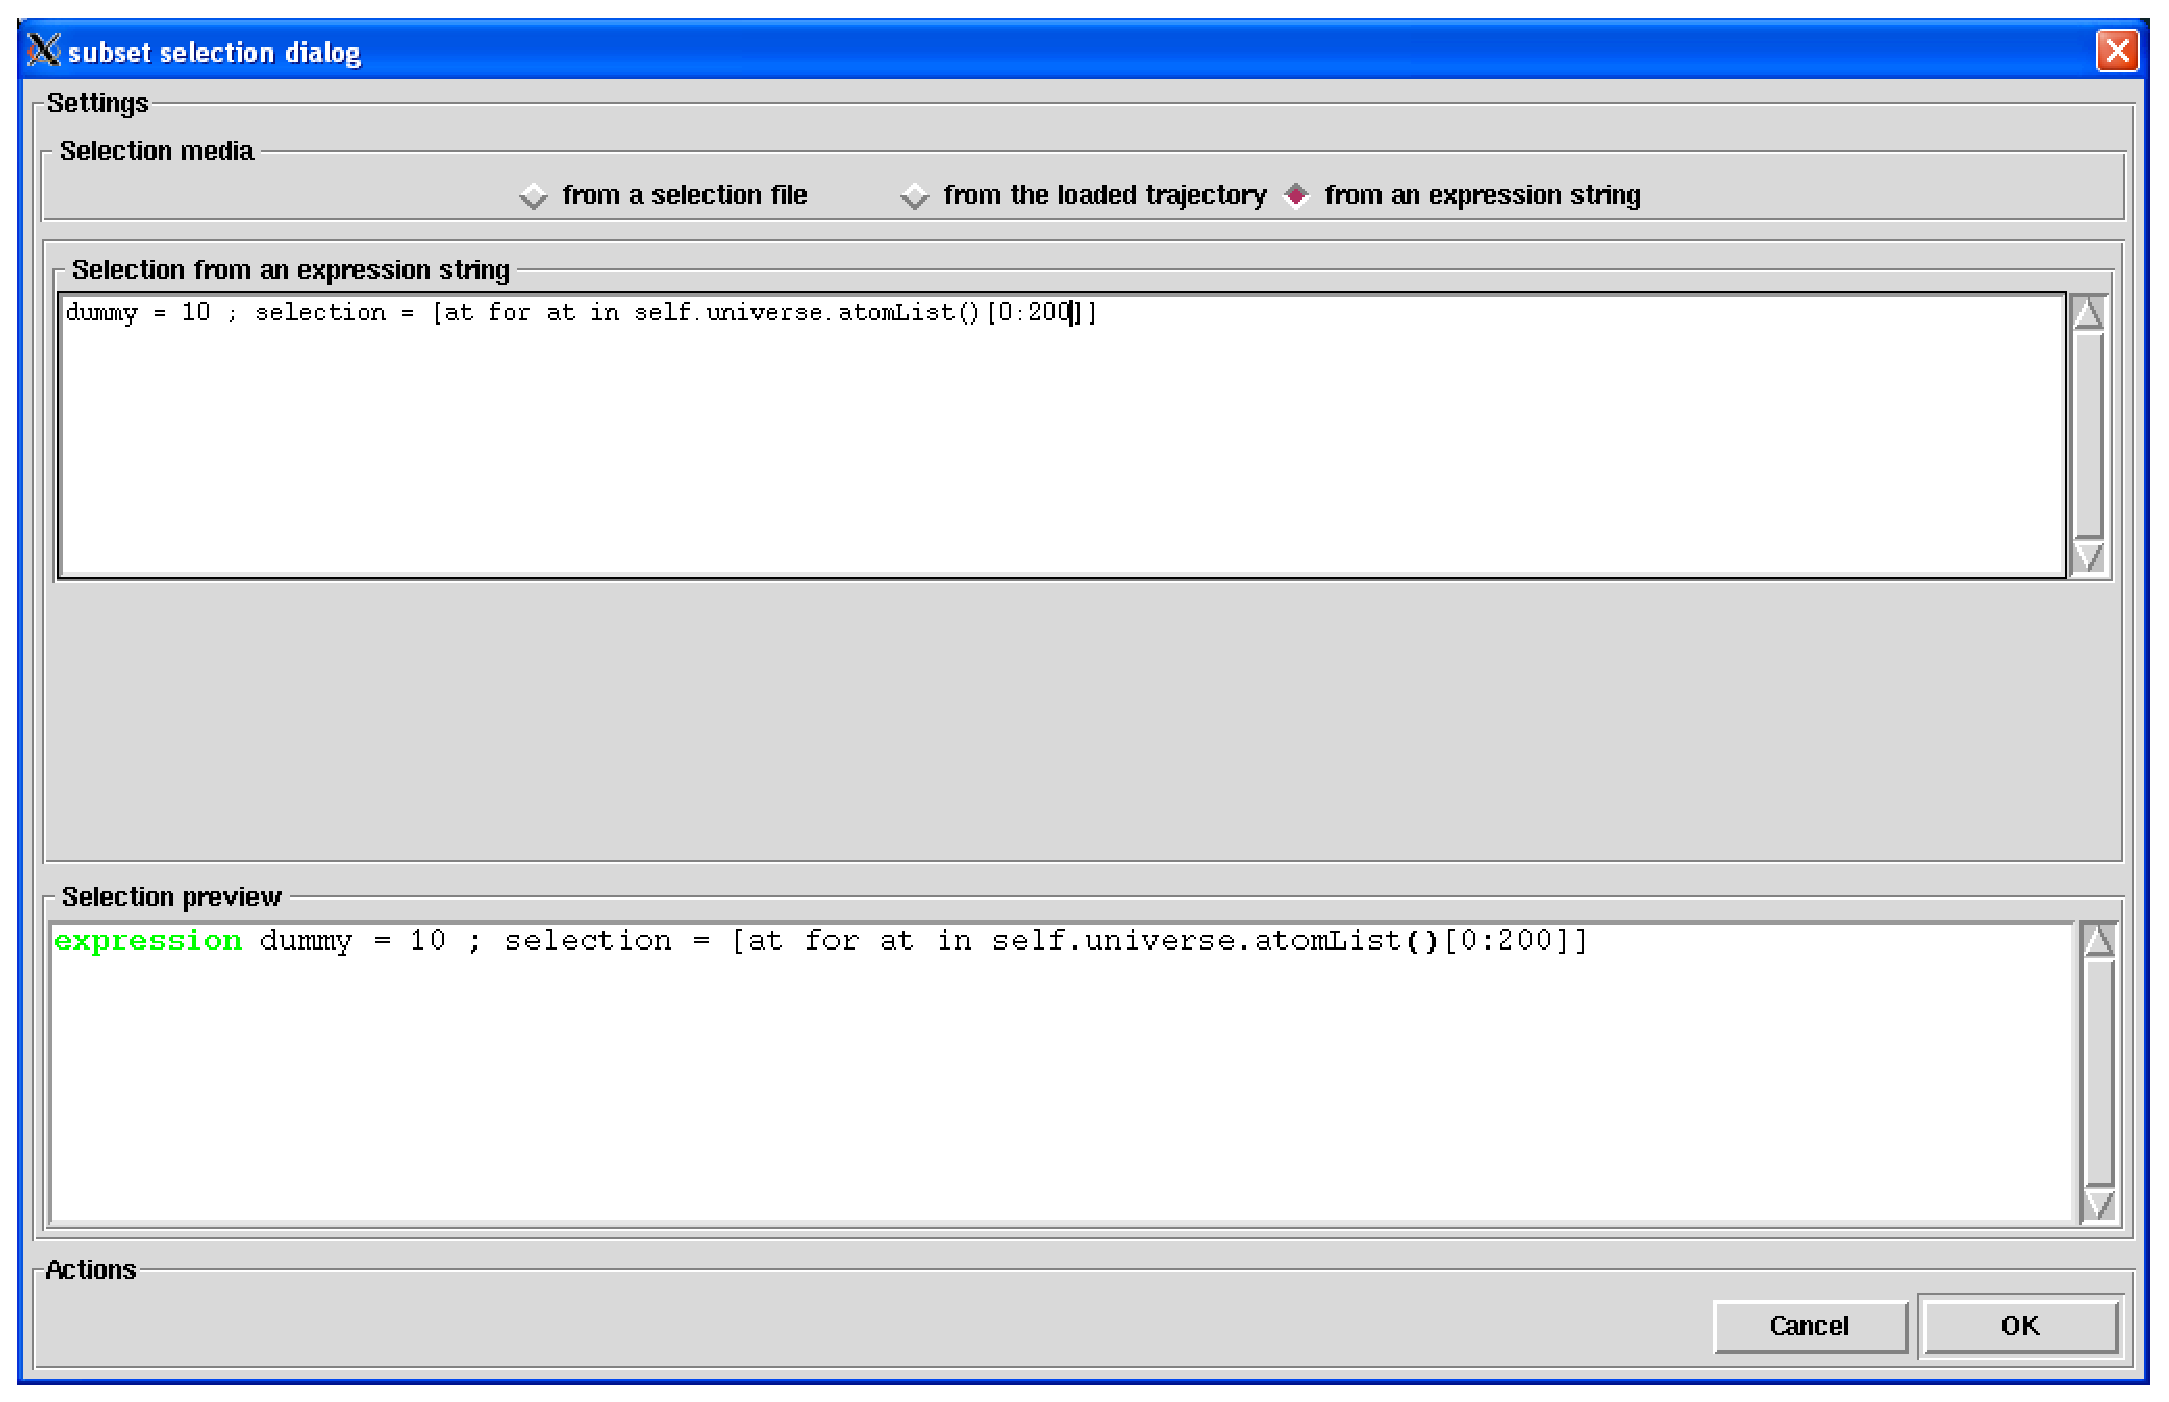
\includegraphics[width=10cm]{Figures/subset_selection_from_an_expression_string.eps}
\end{center}
\caption[The subset selection dialog for a selection from an expression string]{The subset selection dialog for a selection from an expression string.}
\label{fig:subset_selection_from_an_expression_string}
\end{figure}   

Once an expression string has been entered press \textbf{Return} to register it. The constructed selection string that will be used by \NMOLDYN\ for this kind of 
selection will be displayed in the \textbf{Selection preview} entry at the bottom of the dialog with highlighted keywords.

Here are some examples of valid expression strings that can be entered:
\begin{itemize}
\item \textit{selection = self.universe.atomList()[0:10]}: will select the ten first atoms of the universe,
\item \textit{selection = [at for at in self.universe if at.\_mass $\geq$ 10]}: will select only the atoms of the universe whose 
mass is greater than 10 \amu .
\end{itemize}
\newpage
\subsubsection{Deuteration selection}
\label{deuteration_selection}
This kind of selection is useful for analysis if you want to change the parameters (e.g. mass, scattering lengths) of some hydrogens 
atoms to the ones of deuterium. This allows to simulate the system in a fully or partially deuterated state.

By default, \NMOLDYN\ does not select any hydrogen atom for deuteration for an analysis. The dialog from which a deuteration 
selection is performed is displayed in figure \ref{fig:deuteration_selection}.
\begin{figure}[h!]
\begin{center}
\includegraphics[width=10cm]{Figures/deuteration_selection.eps}
\end{center}
\caption[The deuteration selection dialog]{The dialog from where a deuteration selection is performed.}
\label{fig:deuteration_selection}
\end{figure}   

As can be seen from that figure, the deuteration dialog is exactly the same that the subset selection dialog. At the bottom 
of the dialog, the \textbf{Actions} frame contains the \textbf{Cancel} button to cancel the selection and 
the \textbf{OK} button to validate the selecton.

On the top of the dialog, three radiobuttons allows to select from which media the selection will be performed. This can 
be:
\begin{itemize}
\item \textbf{from a selection file}: this will perform the selection from a \NMOLDYN\ deuteration selection file,
\item \textbf{from the loaded trajectory}: this will perform the selection directly from the contents of the universe contained 
in the loaded trajectory,
\item \textbf{from an expression string}: this will perform the selection from a valid python expression declaring a list 
of  atoms to include in the selection.
\end{itemize}
When clicking on one of these radiobutton, a media-specific dialog will be displayed in the underneath frame.

\paragraph{selection from a selection file\\}
\label{deuteration_selection_from_a_selection_file}
To perform a deuteration selection from a selection file, you have to click on the \textbf{from a selection file} radiobutton. 
A dialog will be displayed in the underneath frame from which you will be asked for a deuteration selection file (see 
Fig. \ref{fig:deuteration_selection_from_a_selection_file}).
\newpage
\begin{figure}[h!]
\begin{center}
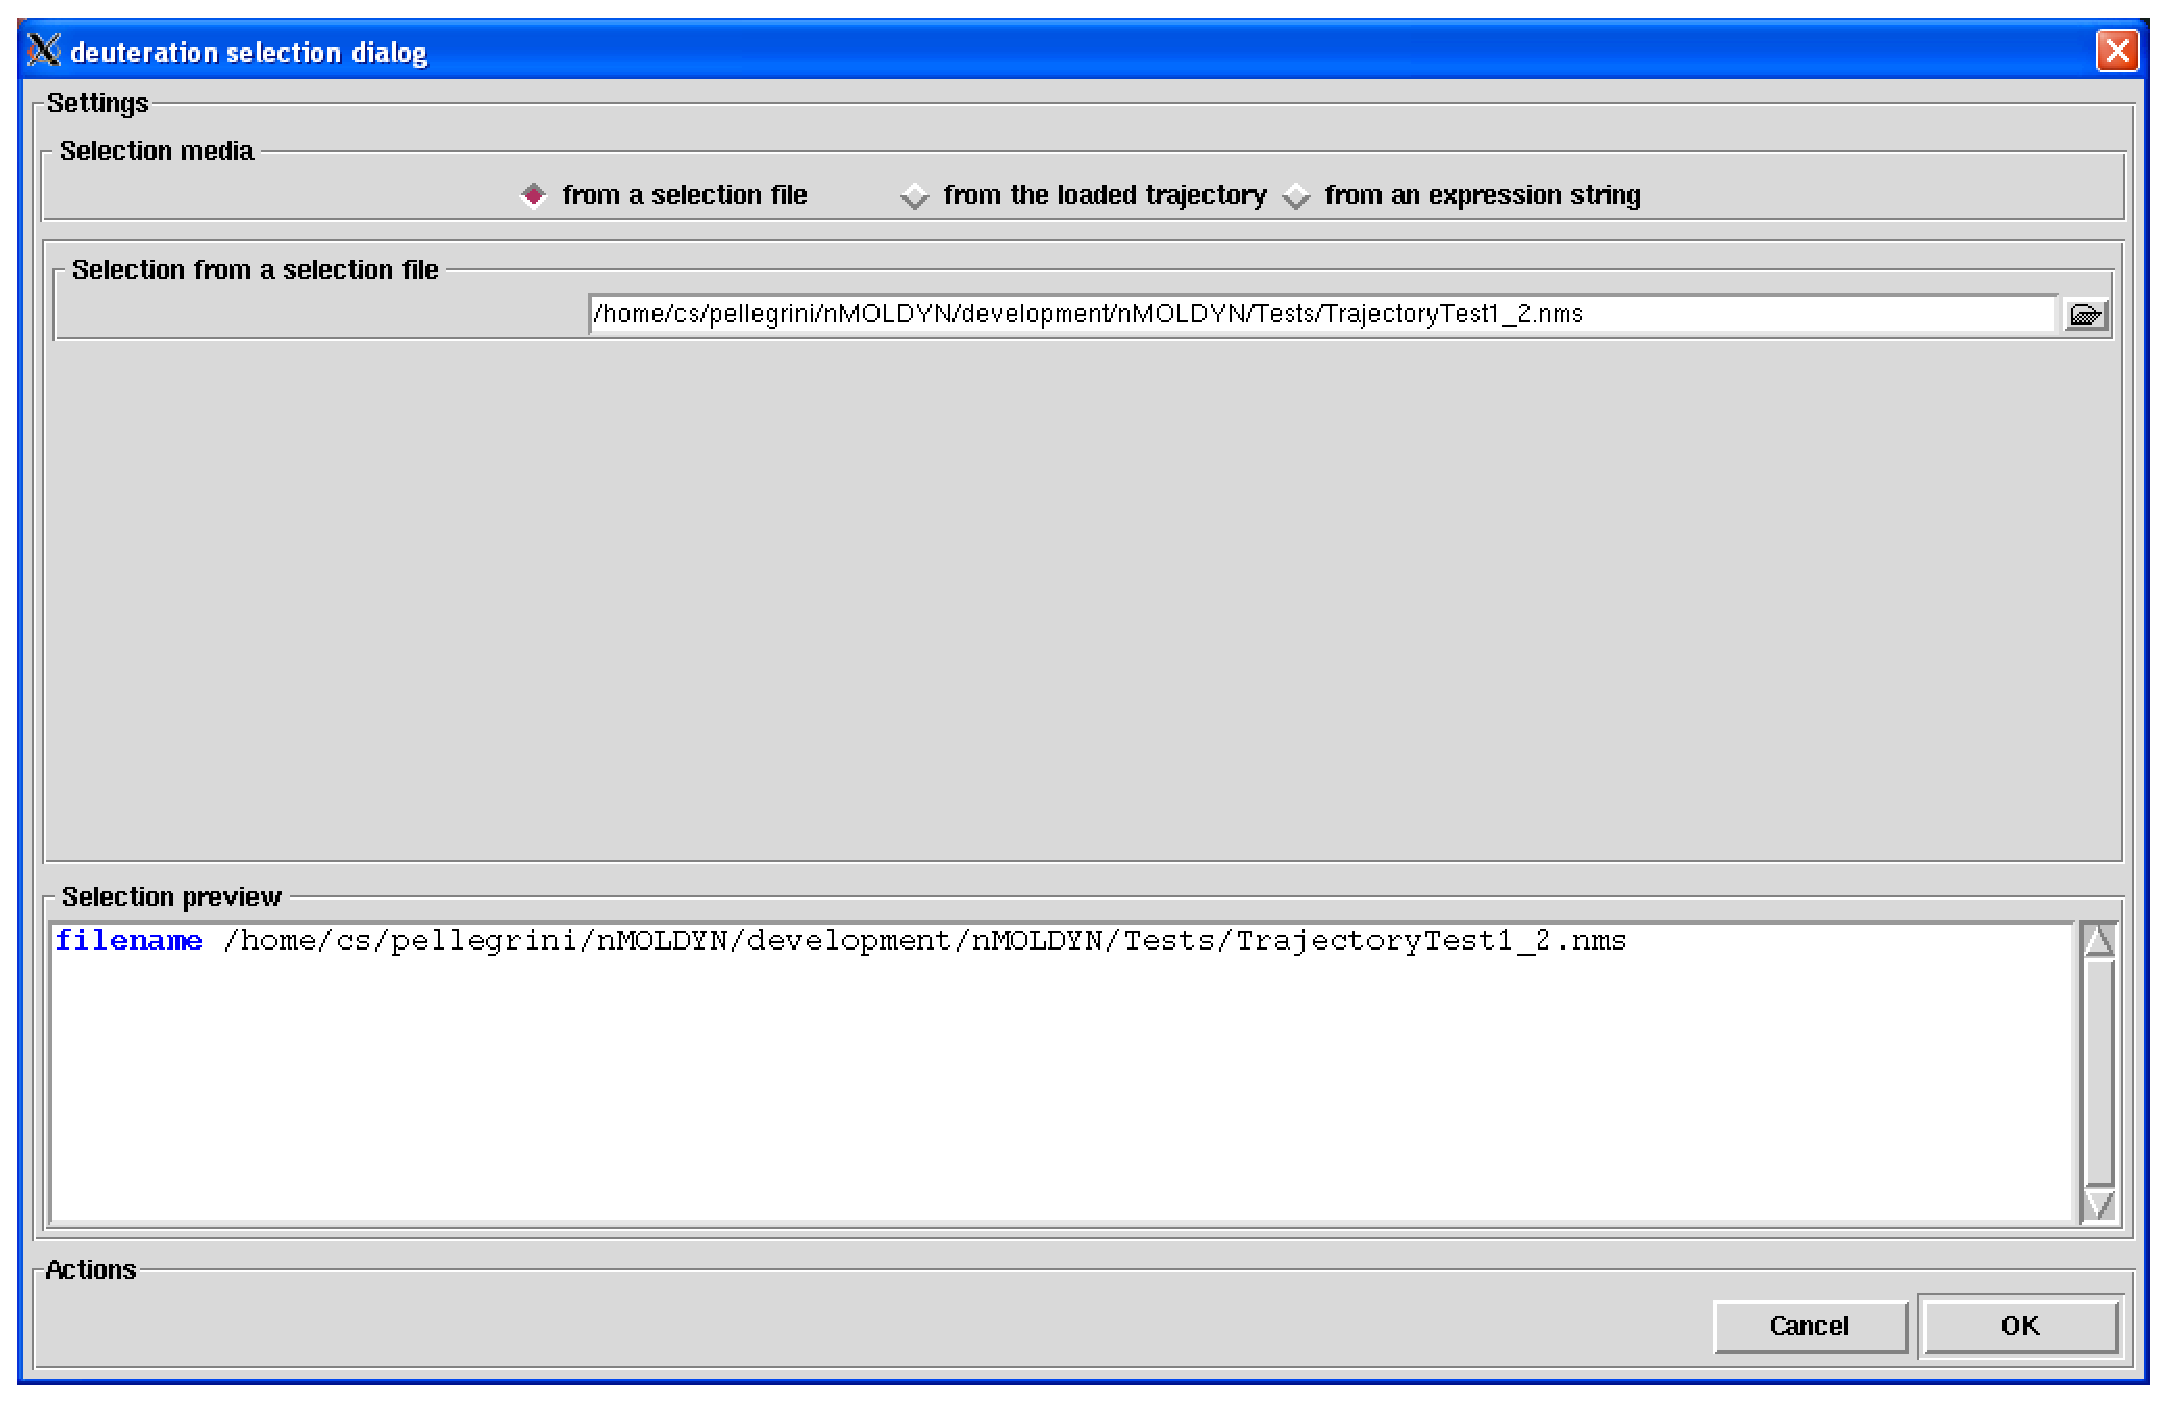
\includegraphics[width=10cm]{Figures/deuteration_selection_from_a_selection_file.eps}
\end{center}
\caption[The deuteration selection dialog for a selection from a selection file]{The deuteration selection dialog for a selection from a selection file.}
\label{fig:deuteration_selection_from_a_selection_file}
\end{figure}   

The format of a \NMOLDYN\ deuteration selection file is quite simple. It is an ASCII file with the \textbf{.nms} extension whose 
contents is a python script made of two lines. The first line must set the variable \textit{pdb} to the path of a \PDB\ file 
of the first frame of the trajectory being processed (it can be obtained using the frame extractor tool described in 
section \ref{frame_snapshot} for example).The second line must set the variable \textit{deuteration} to a list of integers 
where each integers represents the \PDB\ serial number of the atoms to select. An example of a deuteration selection file 
is shown in figure \ref{fig:deuteration_selection_file}.
\begin{figure}[h!]
\begin{center}
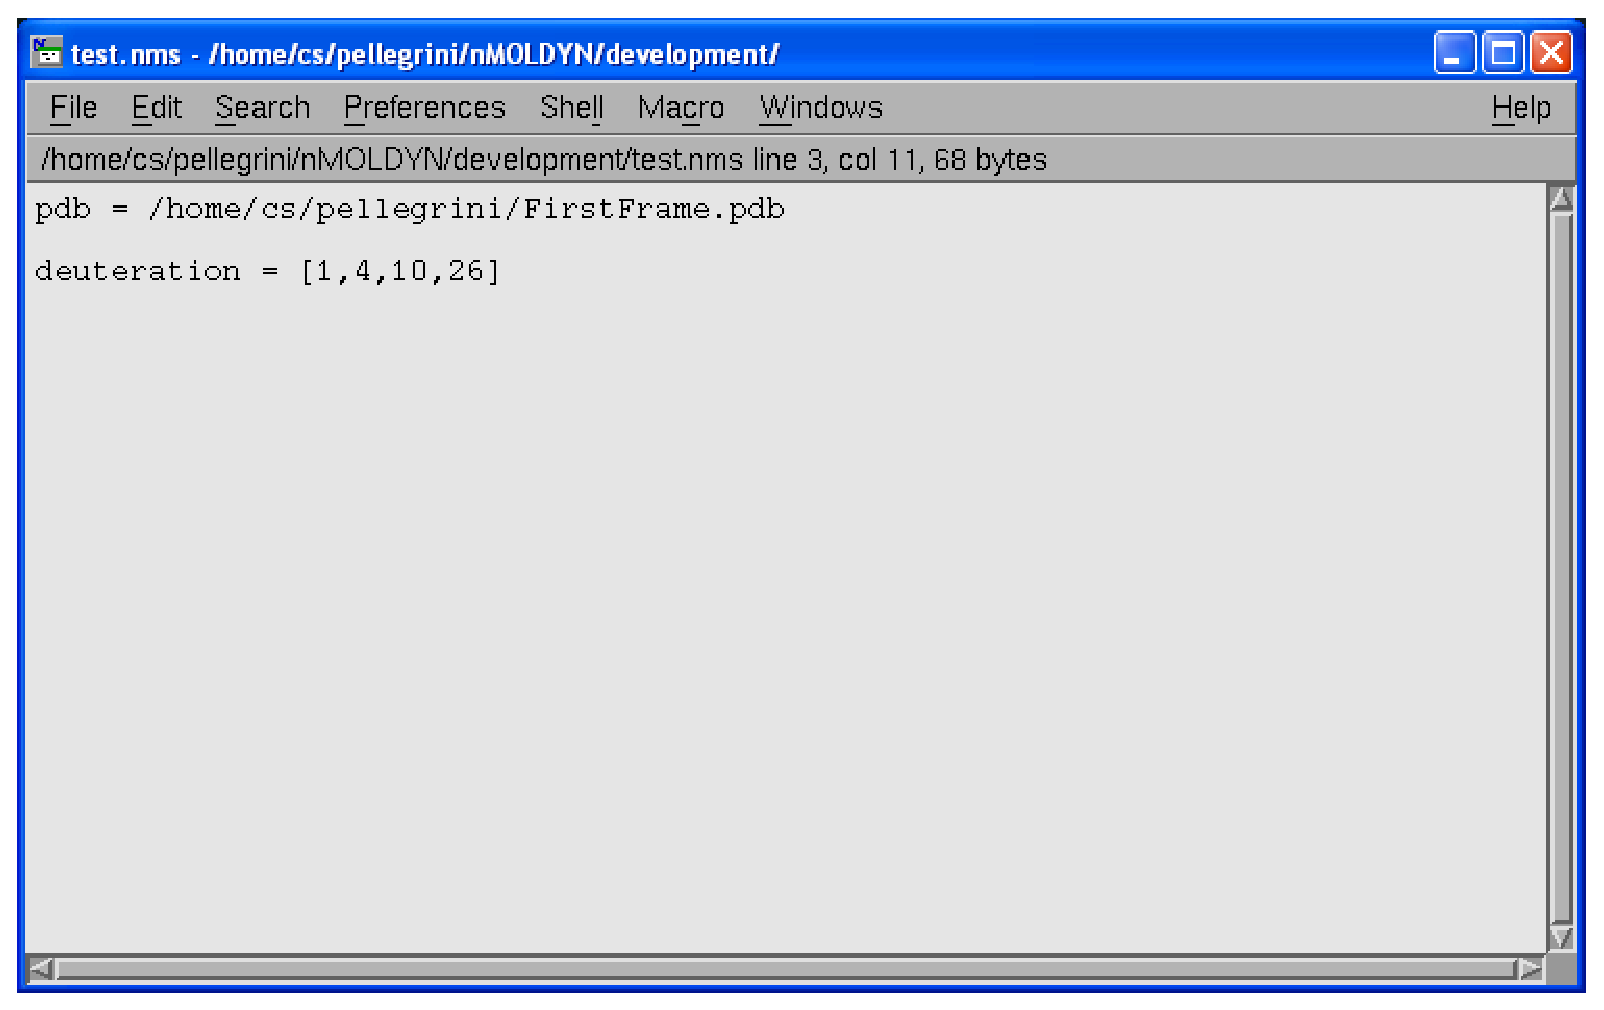
\includegraphics[width=10cm]{Figures/deuteration_selection_file.eps}
\end{center}
\caption[Example of a deuteration selection file]{Example of a deuteration file.}
\label{fig:deuteration_selection_file}
\end{figure}   

Once a selection file has been loaded, the constructed selection string that will be used by \NMOLDYN\ for this kind of 
selection is displayed in the \textbf{Selection preview} entry at the bottom of the dialog with highlighted keywords.
\newpage
\paragraph{selection from the loaded trajectory\\}
To perform a deuteration selection from the loaded trajectory, you have to click on the \textbf{from the loaded trajectory} 
radiobutton. A dialog will be displayed in the underneath frame from which you will construct your selection directly from 
the contents of the universe related to the loaded trajectory (see Fig. \ref{fig:deuteration_selection_from_the_loaded_trajectory}).
\begin{figure}[h!]
\begin{center}
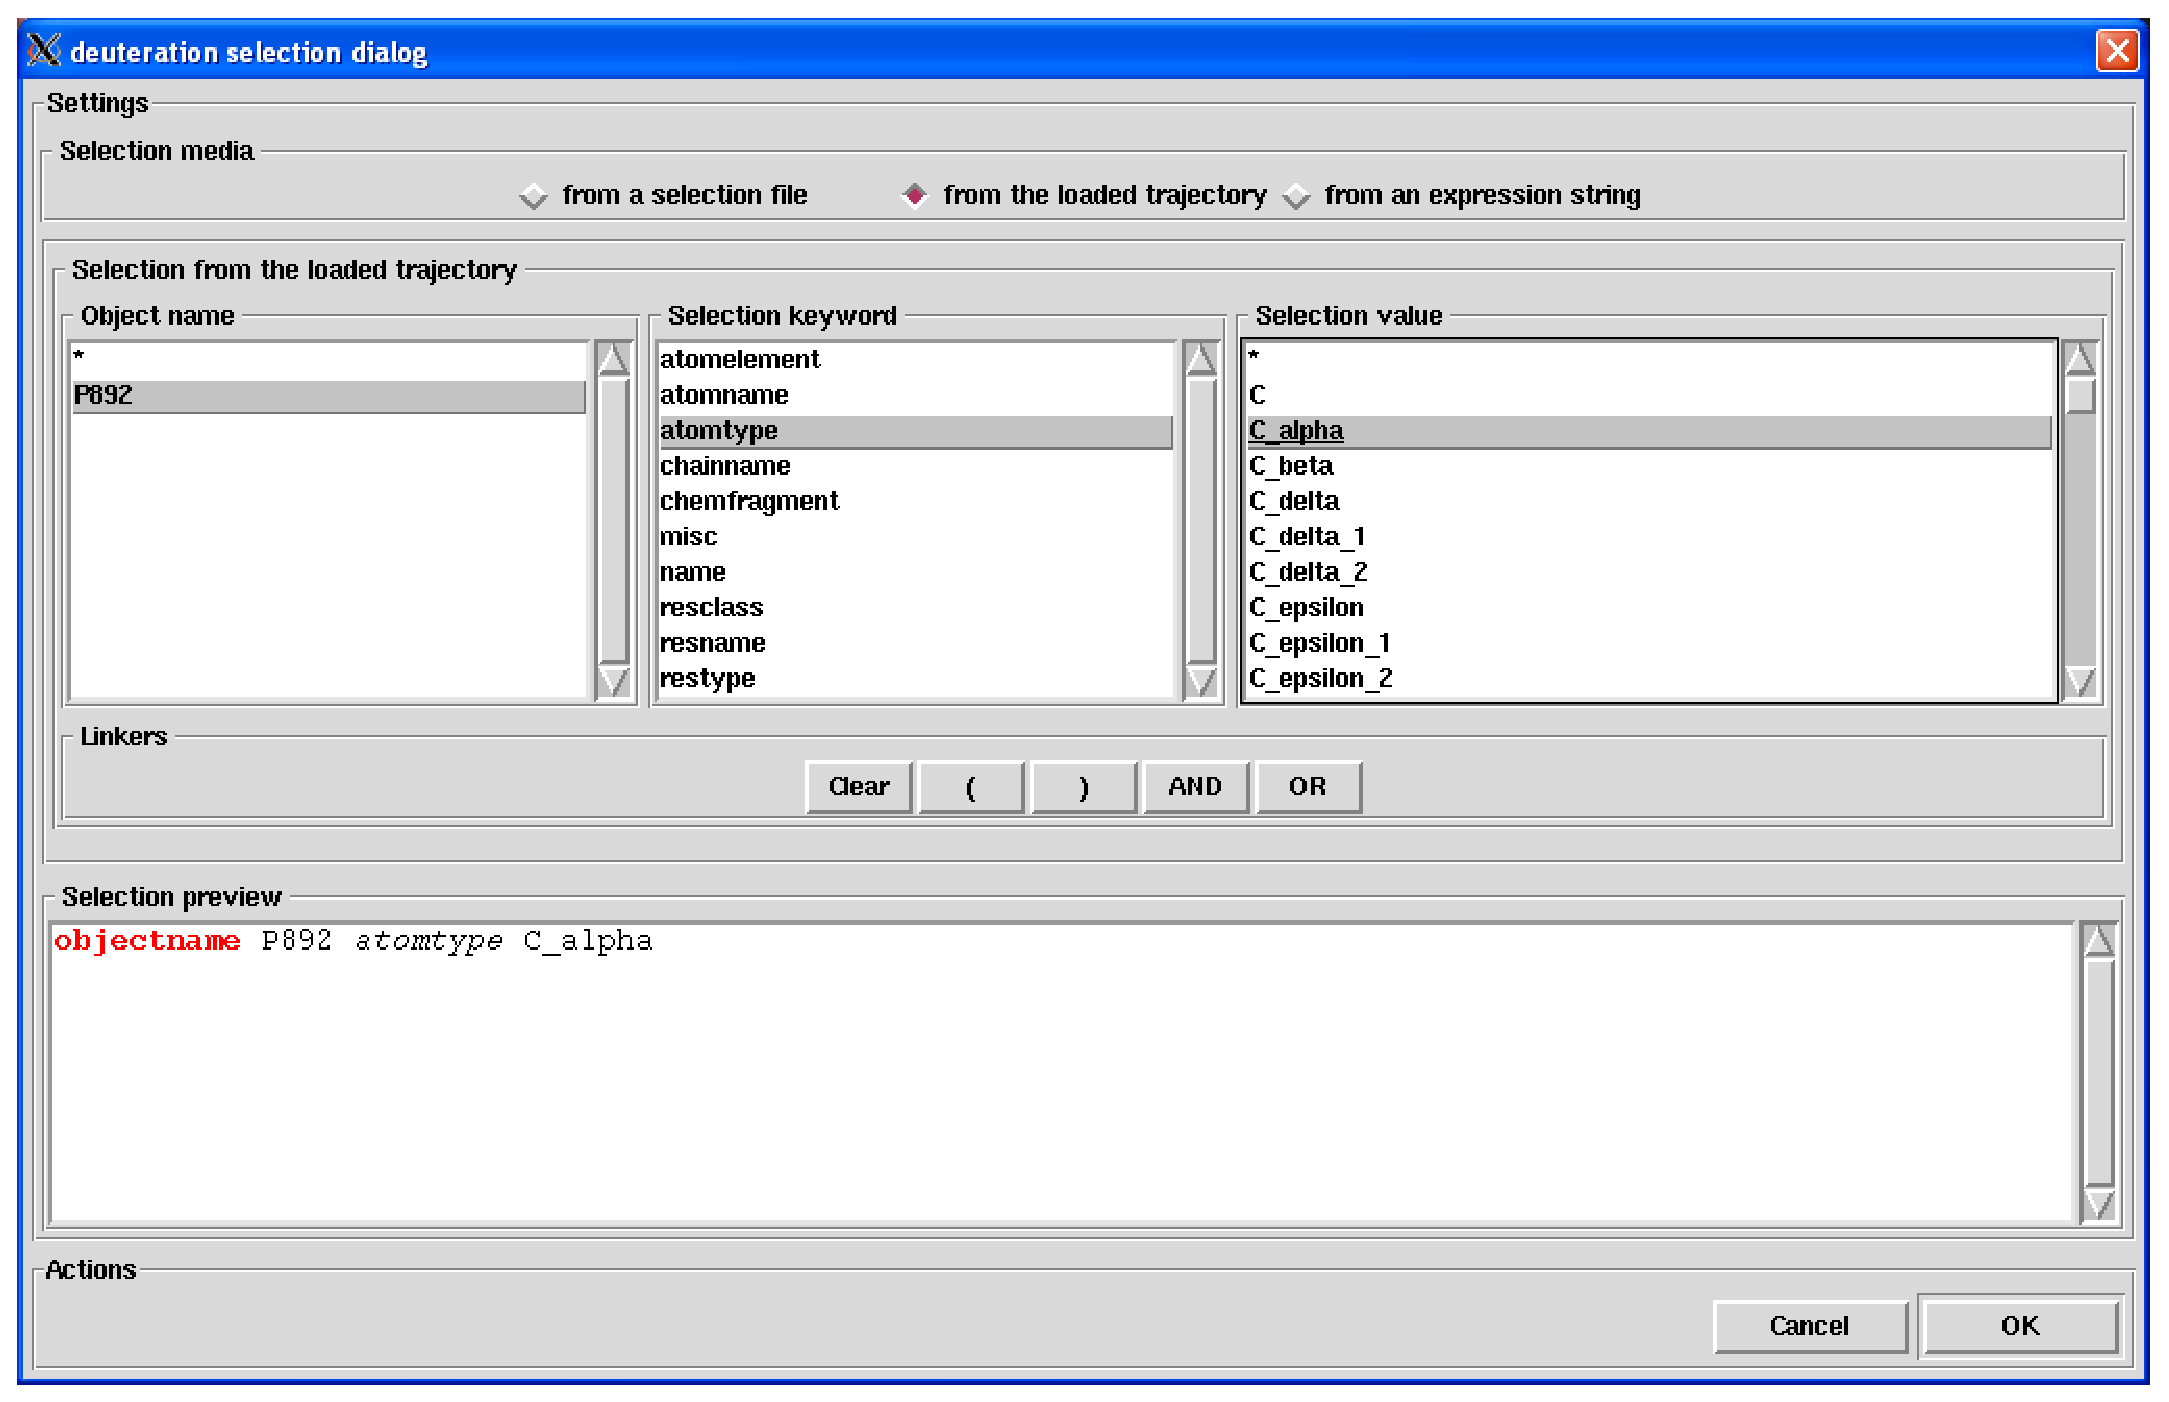
\includegraphics[width=10cm]{Figures/deuteration_selection_from_the_loaded_trajectory.eps}
\end{center}
\caption[The deuteration selection dialog for a selection from the loaded trajectory]{The deuteration selection dialog for a selection from the loaded trajectory.}
\label{fig:deuteration_selection_from_the_loaded_trajectory}
\end{figure}   

To construct the selection, it is compulsory to proceed in the following order:
\begin{enumerate}
\item select an object name among the ones displayed in the \textbf{Object name} listbox. This will 
display in the \textbf{Selection keywords} listbox the selection keywords associated to the selected object.
\item select a selection keyword among the ones displayed in \textbf{Selection keywords} listbox. This will display in the 
\textbf{Selection value} listbox the values associated to the selected keyword.
\item unselect/select one or several values among the ones displayed in the \textbf{Selection value} listbox.
\end{enumerate}
By doing so, you will construct a selection string with the following format:
\\\\
\textit{objectname name keyword value1,value2, \ldots}
\\\\
where \textit{name} is the selected object name (step 1), \textit{keyword} is the selected keyword (step 2) and 
\textit{value1,value2,\ldots} are the selected values (step 3). This constructed selection string, that will be used by 
\NMOLDYN , is displayed in the \textbf{Selection preview} entry at the bottom of the dialog with highlighted keywords. 

You can associate several selection keywords to a given selected object by repeating steps 2,3. In that case, 
the constructed selection string will have the following format:
\\\\
\textit{objectname name keyword1 value1,value2,\ldots OR keyword2, value1,value2,value3\ldots}
\\\\
where the keyword \textit{OR} will be interpreted by \NMOLDYN\ as an union operator in the sense that it will take the 
union between the set of atoms generated by \textit{keyword1 value1,value2}, \textit{keyword2 value1,value2,value3} \ldots

You can also include several objects in the selection by repeating steps 1,2,3. In that case, the constructed selection 
string will have the following format:
\\\\
\textit{objectname name1 keyword1 value1,\ldots OR keyword2, value1,value2, \ldots OR objectname name2 keyword1 value1 \ldots}
\\\\
Finally, using the buttons within the \textbf{Linkers} frame each time a step 3 is completed allows to construct more complex selection strings using the 
\textbf{(}, \textbf{)}, \textbf{AND}, \textbf{OR} linkers, the \textbf{AND} linker acting as an intersection operator while the 
\textbf{OR} link, described above, acts as an union operator. The button \textbf{Clear} clears up the selection string under construction.

The table \ref{tab:selection_keywords} lists the selection keywords and values depending on the \MMTK\ type of the object being processed.

\paragraph{selection from an expression string\\}
To perform a deuteration selection from an expression string, you have to click on the \textbf{from an expression string} 
radiobutton. A dialog will be displayed in the underneath frame from which you will enter a valid Python expression 
that must declare the \textit{selection} variable as a list of atoms of the loaded universe. The variable 
\textit{self.universe} will be used as a reference for that universe (see Fig. \ref{fig:deuteration_selection_from_an_expression_string}).
\begin{figure}[h!]
\begin{center}
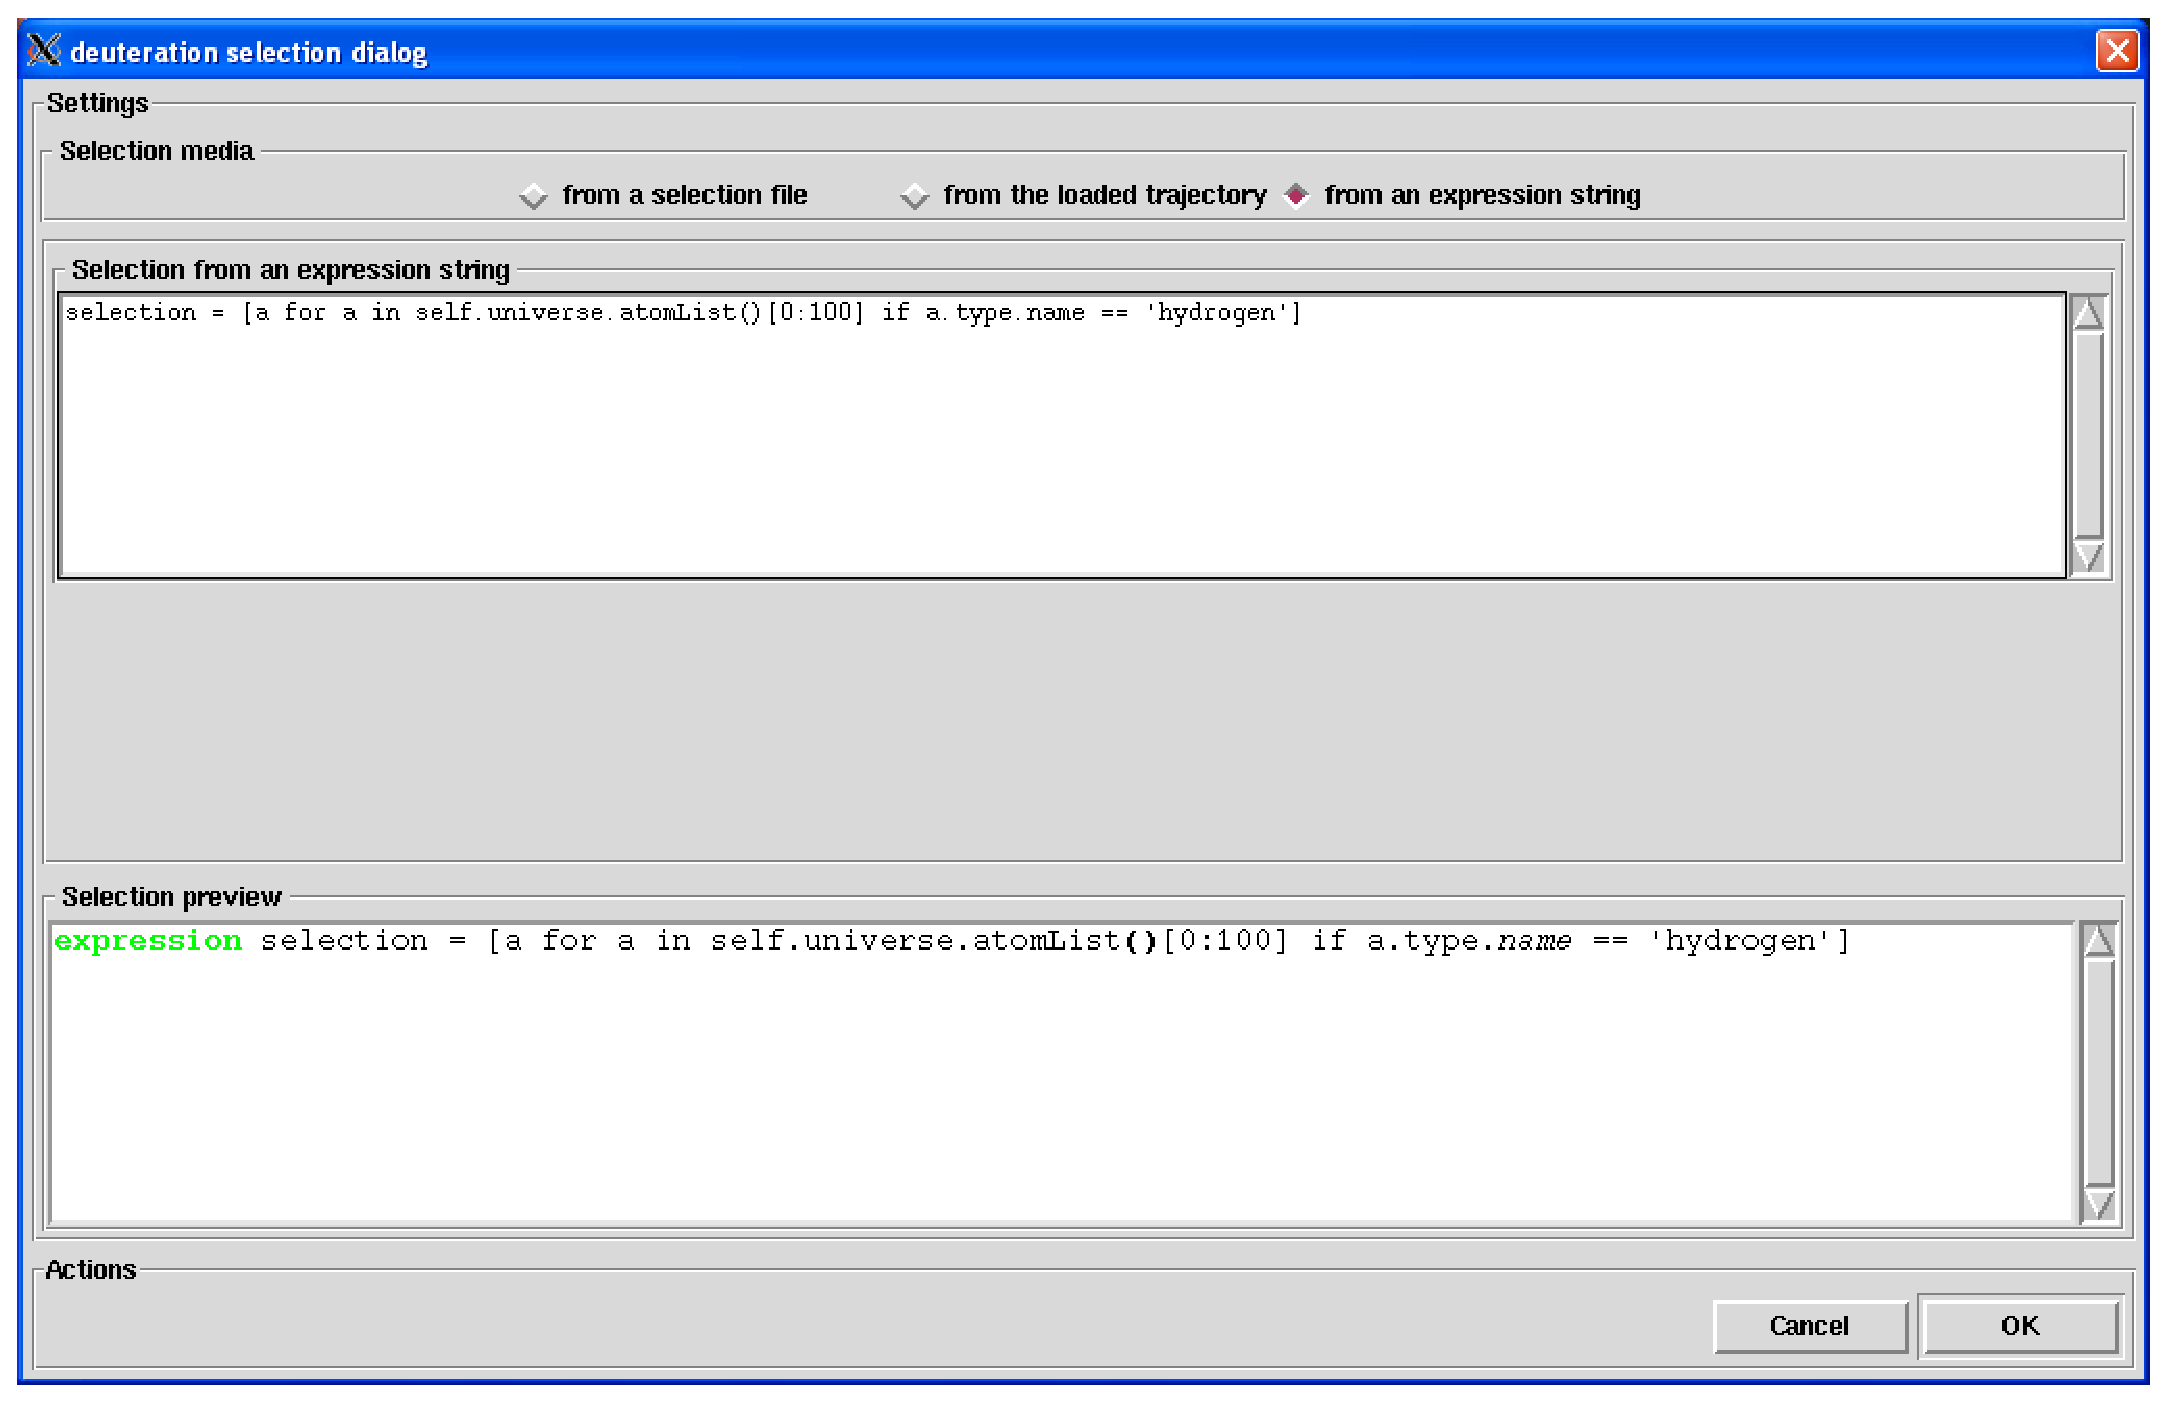
\includegraphics[width=10cm]{Figures/deuteration_selection_from_an_expression_string.eps}
\end{center}
\caption[The deuteration selection dialog for a selection from an expression string]{The deuteration selection dialog for a selection from an expression string.}
\label{fig:deuteration_selection_from_an_expression_string}
\end{figure}   

Once an expression string has been entered press \textbf{Return} to register it. The constructed selection string that will 
be used by \NMOLDYN\ for this kind of selection will be displayed in the \textbf{Selection preview} entry at the bottom of 
the dialog with highlighted keywords.

Whatever the selection media used, in case where non-hydrogens atoms were accidently introduced in the deuteration 
selection, \NMOLDYN\ will filtered them out from the resulting selection.
\newpage
\subsubsection{Group selection}
\label{group_selection}
This kind of selection is especially desgned for analysis based on group of atoms on which a given operation is performed 
collectively. By collectively, we mean that the selected group of atoms will be treated as it was one object. For example, 
in rigid-body based analysis, selecting a group of atoms will mean that this group will be considered as a single rigid-body 
that will be used to derve the rigid-body trajectory. Another example, the study where one needs to define the center of mass 
of a group of atoms in order to derive a property such as coordination number or spatial density (see Sections \ref{cn} and 
\ref{sd}). In that case, a center of mass will be defined for each selected group of atoms.

By default, \NMOLDYN\ consider all the atoms for a group selection. The dialog from which a group selection is performed is 
displayed in figure \ref{fig:group_selection}.
\begin{figure}[h!]
\begin{center}
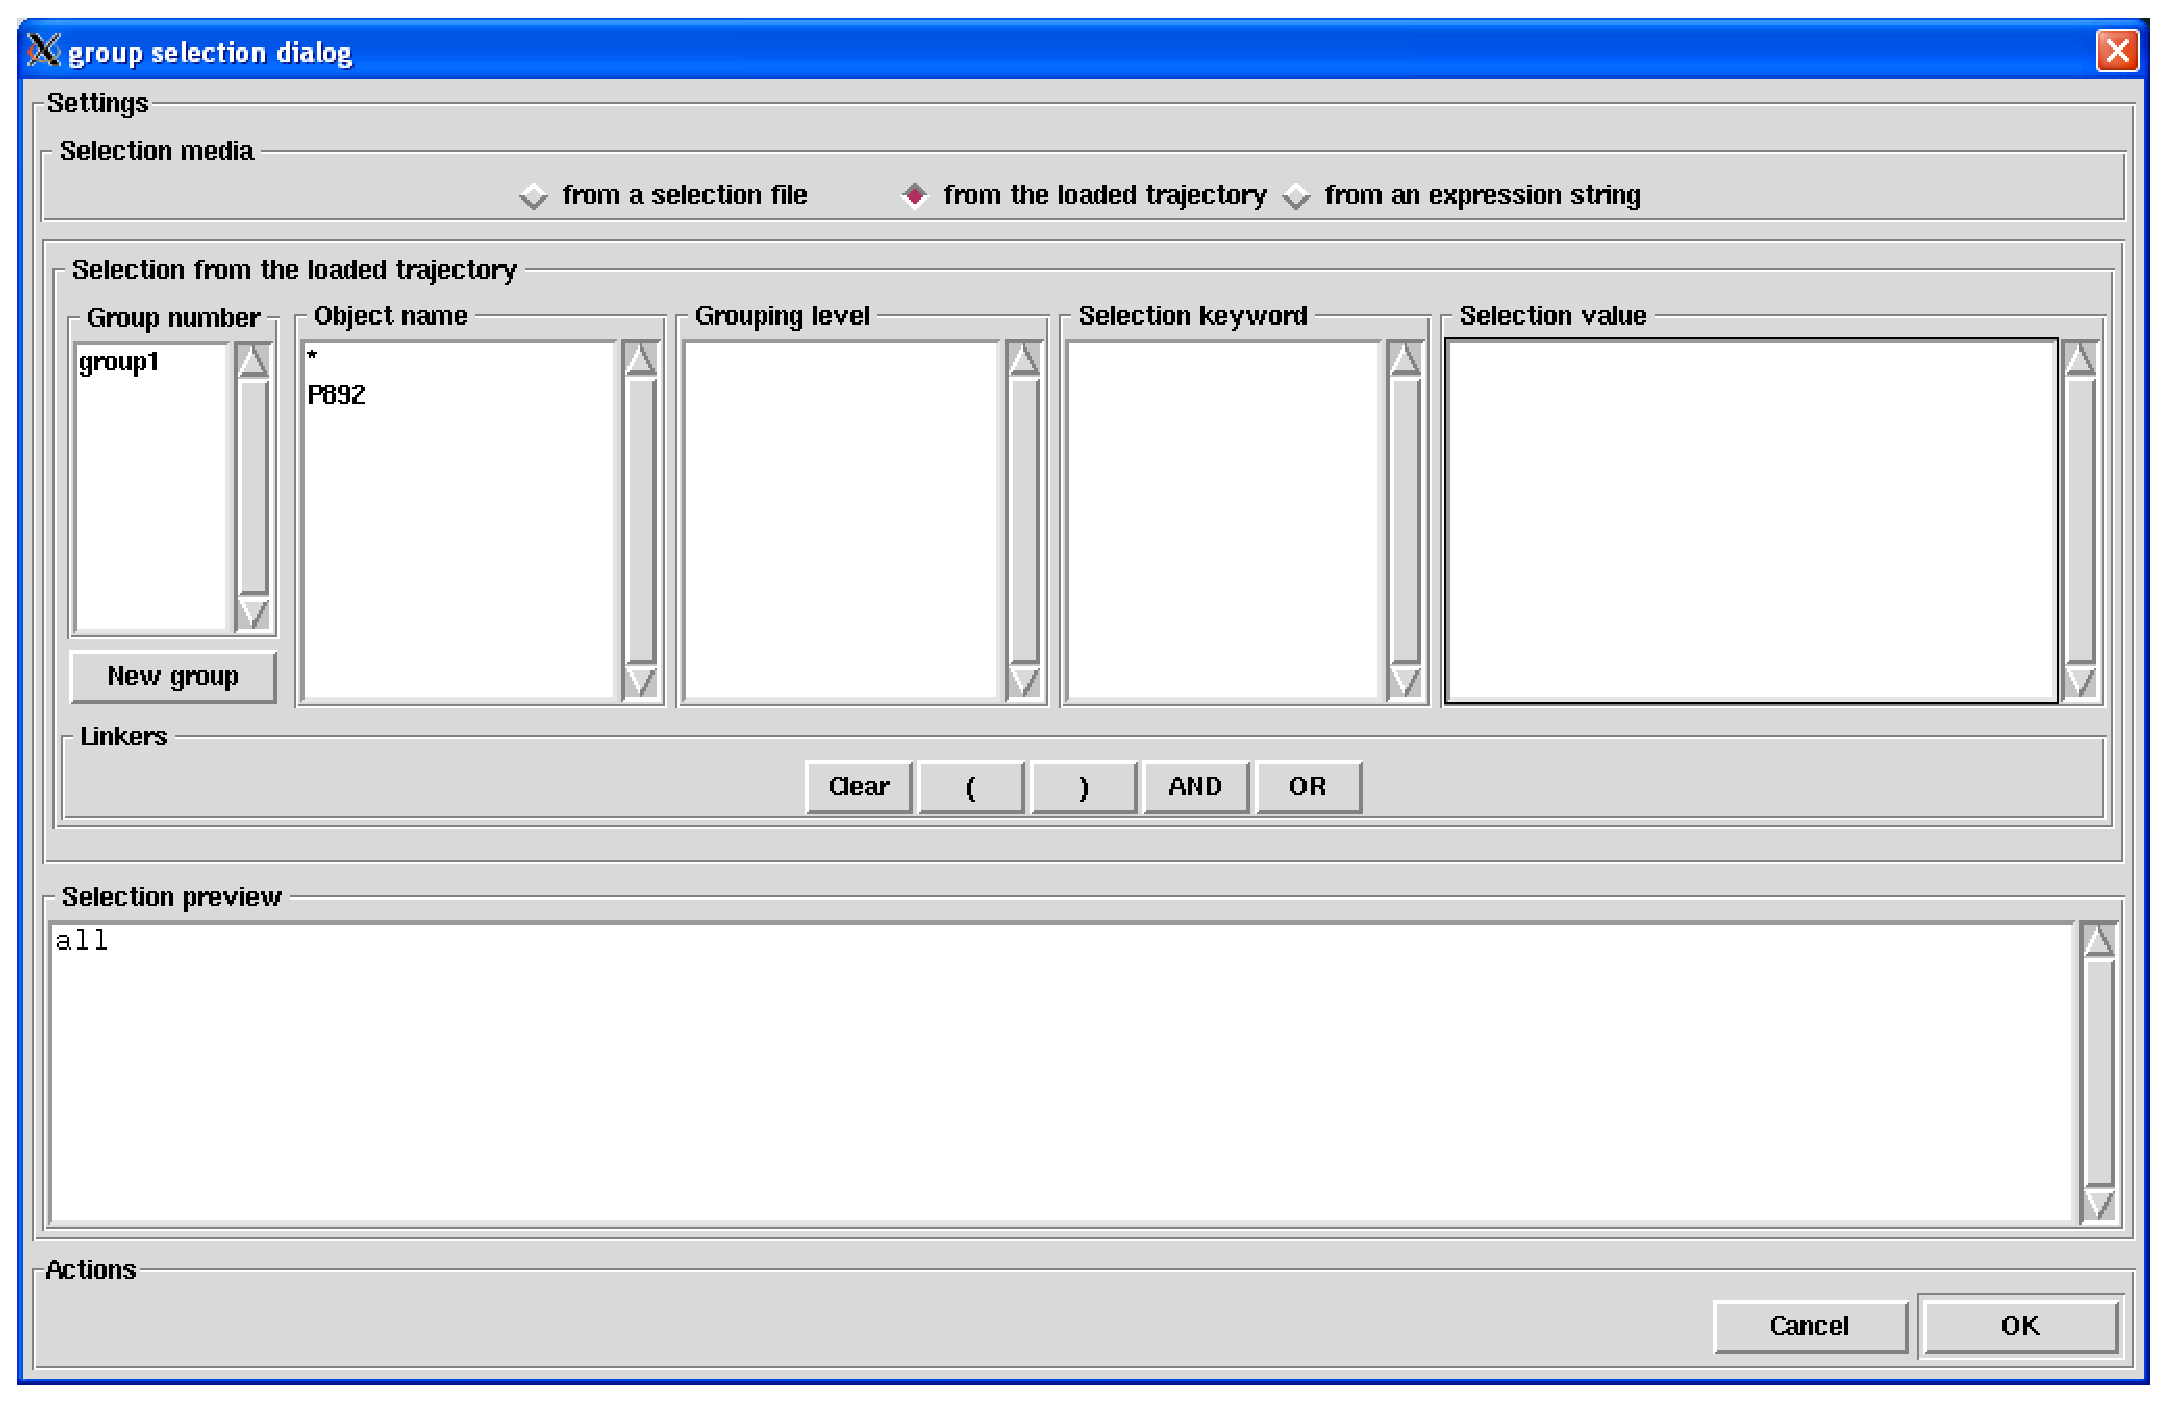
\includegraphics[width=10cm]{Figures/group_selection.eps}
\end{center}
\caption[The group selection dialog]{The dialog from where a group selection is performed.}
\label{fig:group_selection}
\end{figure}   

At the bottom of the dialog, the \textbf{Actions} frame contains the \textbf{Cancel} button to cancel the selection and 
the \textbf{OK} button to validate the selecton.

On the top of the dialog, three radiobuttons allows to select from which media the selection will be performed. This can be:
\begin{itemize}
\item \textbf{from a selection file}: this will perform the selection from a \NMOLDYN\ group selection file,
\item \textbf{from the loaded trajectory}: this will perform the selection directly from the contents of the universe contained 
in the loaded trajectory,
\item \textbf{from an expression string}: this will perform the selection from a valid python expression declaring a list 
of  atoms to include in the selection.
\end{itemize}
When clicking on one of these radiobutton, a media-specific dialog will be displayed in the underneath frame.
\newpage
\paragraph{selection from a selection file\\}
\label{group_selection_from_a_selection_file}
To perform a group selection from a selection file, you have to click on the \textbf{from a selection file} radiobutton. 
A dialog will be displayed in the underneath frame from which you will be asked for a group selection file 
(see Fig. \ref{fig:group_selection_from_a_selection_file}).
\begin{figure}[h!]
\begin{center}
\includegraphics[width=10cm]{Figures/group_selection_from_a_selection_file.eps}
\end{center}
\caption[The group selection dialog for a selection from a selection file]{The group selection dialog for a selection from a selection file.}
\label{fig:group_selection_from_a_selection_file}
\end{figure}   

The format of a \NMOLDYN\ group selection file is quite simple. It is an ASCII file with the \textbf{nms} extension whose 
contents is a python script made of two lines. The first line must set the variable \textit{pdb} to the path of a \PDB\ file 
of the first frame of the trajectory being processed (it can be obtained using the frame extractor tool described in 
section \ref{frame_snapshot} for example).The second line must set the variable \textit{deuteration} to nested lists of 
integers where each nested list will generate a group of atoms whose \PDB\ serial number match the integer of the nested list. 
An example of a deuteration selection file is shown in figure \ref{fig:group_selection_file}.
\begin{figure}[h!]
\begin{center}
\includegraphics[width=10cm]{Figures/group_selection_file.eps}
\end{center}
\caption[Example of a group selection file]{Example of a group file.}
\label{fig:group_selection_file}
\end{figure}   

This example will create three groups. The first one made of atoms 1, 4, 9, 78, 101 and 134 of the \PDB\ file, the second one made of the 
atoms 12, 23 and 192 and the third one made of the atoms 11, 26, 1023, 245 and 234.

Once a selection file has been loaded, the constructed selection string that will be used by \NMOLDYN\ for this kind of 
selection is displayed in the \textbf{Selection preview} entry at the bottom of the dialog with highlighted keywords.

\paragraph{selection from the loaded trajectory\\}
To perform a group selection from the loaded trajectory, you have to click on the \textbf{from the loaded trajectory} 
radiobutton. A dialog will be displayed in the underneath frame from which you will construct your selection directly from 
the contents of the universe related to the loaded trajectory (see Fig. \ref{fig:group_selection_from_the_loaded_trajectory}).
\begin{figure}[h!]
\begin{center}
\includegraphics[width=10cm]{Figures/group_selection_from_the_loaded_trajectory.eps}
\end{center}
\caption[The group selection dialog for a selection from the loaded trajectory]{The group selection dialog for a selection from the loaded trajectory.}
\label{fig:group_selection_from_the_loaded_trajectory}
\end{figure}   

To construct the selection, it is compulsory to proceed in the following order:
\begin{enumerate}
\item create a new type of group by clicking on \textbf{New group} button or overwrite an existing one by selecting it in the \textbf{Group number} listbox,
\item select an object name among the ones displayed in the \textbf{Object name} listbox. This will 
display the grouping levels associated to the selected object in the \textbf{Grouping level} listbox and the selection 
keywords associated to the selected object in the \textbf{Selection keywords} listbox,
\item select a grouping level among the ones displayed in the \textbf{Grouping level} listbox. This is specific to group 
selection as when selecting a group of atoms, you must specify at which level the selected atoms will be grouped. For example, if you perform a group selection on a protein. If you set the grouping 
level to \textit{protein}, then the group will be the whole protein. But, if you set the grouping level to \textit{residue}, then
the group selection will results on a set of $N_{residues}$ group where $N_{residues}$ is the number of residues of the 
protein.
\item select a selection keyword among the ones displayed in \textbf{Selection keywords} listbox. This will display in the 
\textbf{Selection value} listbox the values associated to the selected keyword.
\item unselect/select one or several values among the ones displayed in the \textbf{Selection value} listbox.
\end{enumerate}
\newpage
By doing so, you will construct a selection string with the following format:
\\\\
\textit{group1 groupinglevel level objectname name keyword value1,value2, \ldots}
\\\\
where \textit{group1} is the name of the group, \textit{level} is the selected grouping level, \textit{name} is the selected object name (step 1), \textit{keyword} is the selected keyword (step 2) and 
\textit{value1,value2,\ldots} are the selected values (step 3). This constructed selection string is displayed in the \textbf{Selection preview} entry at the bottom of the dialog with highlighted keywords. 

You can associate several selection keywords to a given selected object by repeating steps 2,3. In that case, 
the constructed selection string will have the following format:
\\\\
\textit{group1 groupinglevel level objectname name keyword1 value1,value2,\ldots OR keyword2, value1,value2,value3\ldots}
\\\\
where the keyword \textit{OR} will be interpreted by \NMOLDYN\ as an union operator in the sense that it will take the 
union between the set of atoms generated by \textit{keyword1 value1,value2}, \textit{keyword2 value1,value2,value3} \ldots

You can also include several objects in the selection by repeating steps 1,2,3. In that case, the constructed selection 
string will have the following format:
\\\\
\textit{group1 groupinglevel level objectname name1 keyword1 value1,\ldots OR keyword2, value1,value2, \ldots OR objectname name2 keyword1 value1 \ldots}
\\\\
Finally, using the buttons within the \textbf{Linkers} frame each time a step 3 is completed allows to construct more complex selection strings using the 
\textbf{(}, \textbf{)}, \textbf{AND}, \textbf{OR} linkers, the \textbf{AND} linker acting as an intersection operator while the 
\textbf{OR} link, described above, acts as an union operator. The button \textbf{Clear} clears up the selection string under construction.

The table \ref{tab:selection_keywords} lists the selection keywords and values depending on the \MMTK\ type of the object being processed.

Here are some examples of group selection strings constructed from a protein whose name is P892 and whose number of residues 
is 58:
\begin{itemize}
\item \textit{group1 groupinglevel residue objectname P892 atomelement carbon}: will create 58 groups made of the carbon atoms of 
each residue,
\item \textit{group1 groupinglevel protein objectname P892 atomelement carbon,hydrogen}: will create 1 group made of the carbon 
and hydrogens of the whole protein,
\item \textit{group1 groupinglevel amine objectname P892 atomelement nitrogen group2 groupinglevel hydroxy objectname P892 atomelement oxygen}: 
will create two families of groups. The first one contains groups made of the nitrogen atom of the each amine group of the protein. 
The second one contains groups made of the oxygen atom of the each hydroxy group of the protein. 
\end{itemize}

\paragraph{selection from an expression string\\}
To perform a group selection from an expression string, you have to click on the \textbf{from an expression string} 
radiobutton. A dialog will be displayed in the underneath frame from which you will enter a valid Python expression 
that must declare the \textit{selection} variable as nested lists of atoms of the loaded universe. The variable 
\textit{self.universe} will be used as a reference for that universe (see Fig. \ref{fig:group_selection_from_an_expression_string}).
\newpage
\begin{figure}[h!]
\begin{center}
\includegraphics[width=10cm]{Figures/group_selection_from_an_expression_string.eps}
\end{center}
\caption[The group selection dialog for a selection from an expression string]{The group selection dialog for a selection from an expression string.}
\label{fig:group_selection_from_an_expression_string}
\end{figure}   

Here are some examples of valid expression strings that can be entered:
\begin{itemize}
\item \textit{selection = self.universe.objectList[0].atomList()}: will pack all the atoms of the first object of the universe in one group,
\item \textit{selection = [o.atomList()[0:10] for o in self.universe.objectList()]}: will create a distinct group for each 
object of the universe with its ten first atoms.
\end{itemize}

Once an expression string has been entered press \textbf{Return} to register it. The constructed selection string that will 
be used by \NMOLDYN\ for this kind of selection will be displayed in the \textbf{Selection preview} entry at the bottom of 
the dialog with highlighted keywords.

\subsection{Running modes}
\label{running_modes}
All the analysis dialogs in \NMOLDYN\ contains a frame called \textbf{Actions} located at the bottom of the dialog. That 
frame contains the buttons
\begin{itemize}
\item Cancel,
\item Estimate,
\item Save,
\item Run,
\item Save And Run.
\end{itemize}
The \textbf{Cancel} button cancel the analysis and close the dialog. The \textbf{Estimate} button performs just a single step of the 
analysis and pops up a message box with the estimated time for the full analysis. Not all the analysis can be estimated. In that case, the 
popped up message will inform you that the analysis is not estimable. The \textbf{Save} button pops up a 
dialogs from where you can save the analysis settings either to a \NMOLDYN\ autostart file either to a \NMOLDYN\ input file.
The \textbf{Run} button runs the analysis directly from the \GUI\ and finally the \textbf{Save \& and Run} combinates the actions of 
\textbf{Save} and \textbf{Run} buttons.

\subsection{The Dynamics menu}
\label{dynamics_menu}
Pressing the button \textbf{Dynamics} brings up a menu from which it is possible to choose the following analysis:
\begin{itemize}
\item Mean-Square Displacement
\item Root Mean-Square Displacement
\item Radius Of Gyration
\item Velocity AutoCorrelation Function
\item Density Of States
\item Pass-Band Filtered Trajectory
\item Global Motion Trajectory
\item Center Of Mass Trajectory
\item Rigid-Body Trajectory
\item Center Of Mass Trajectory
\item Auto-Regressive Analysis
\item Quasi-Harmonic Analysis
\item Reorientational Correlation Function
\item Angular Velocity AutoCorrelation Function
\item Angular Density Of States
\end{itemize}

\subsubsection{Mean-Square Displacement}
\label{msd}
\paragraph{Theory and implementation\\}
\label{msd_theory}
Molecules in liquids and gases do not stay in the same place, but move constantly. 
This process is called diffusion and it happens quite naturally in fluids at equilibrium. 
During this process, the motion of an individual molecule does not follow a simple path \cite{Democritus}. 
As it travels, the molecule undergoes some collisions with other molecules which prevent 
it from following a straight line. If the path is examined in close detail, it will be seen 
to be a good approximation to a random walk. Mathematically, a random walk is a series of steps 
where each step is taken in a completely random direction from the one before. 
This kind of path was famously analysed by Albert Einstein in a study of Brownian motion. He showed 
that the \MSD\ of a particle following a random walk is 
proportional to the time elapsed. This relationship can be written as
\begin{equation}
<r^2> = 6Dt + C
\end{equation}
where $<r^2>$ is the \MSD\ and \textit{t} is the time. \textit{D} and \textit{C} are constants. 
The constant \textit{D} defines the so-called diffusion coefficient.
\newpage
The figure \ref{fig:msd_water} shows an example of a \MSD\ analysis performed on a waterbox of 768 water molecules.
\begin{figure}[h!]
\begin{center}
\includegraphics[width=10cm]{Figures/msd_water.eps}
\end{center}
\caption[Examples of calculated \textit{MSD} with \NMOLDYN]{\textit{MSD} calculated for a 100 ps MD simulation of 256 water molecules using NPT condition at 1 bar and 300 K.}
\label{fig:msd_water}
\end{figure}

To get the diffusion coefficient out of this plot, the slope of the linear part of the plot should be calculated.

Defining,
\begin{equation}
\textbf{d}_{\alpha}(t,t_0) \doteq \textbf{R}_\alpha(t_0 + t) - \textbf{R}_\alpha(t_0).
\end{equation}
the \MSD\ of particle $\alpha$ can be defined as:
\begin{equation}
\label{eq:msd}
\Delta^2_\alpha(t) = \left\langle \textbf{d}^2_\alpha(t,t_0) \right\rangle_{t_0}
\end{equation}
where $\textbf{R}_\alpha(t_0)$ and $\textbf{R}_\alpha(t_0 + t)$ are respectively the position of particle $\alpha$ at 
times $t_0$ and $t_0+t$.
One can introduce a \MSD\ with respect to a given axis \textbf{n}:
\begin{equation}
\label{eq:msd_n}
\Delta^2_\alpha(t,t_0;\textbf{n}) \doteq \left\langle
d^2_\alpha(t,\tau;\textbf{n})\right\rangle_{t_0}
\end{equation}
with
\begin{equation}
d_{\alpha}(t,t_0;\textbf{n}) \doteq \textbf{n}\cdot \textbf{d}_{\alpha}(t,t_0).
\end{equation}
The calculation of \MSD\ is the standard way
to obtain diffusion coefficients from \MD\ simulations. Assuming
Einstein-diffusion in the long time limit one has for isotropic
systems
\begin{equation}
\label{eq:diffusion_coeff}
D_\alpha = \lim_{t\to\infty} \frac{1}{6t} \Delta^2_\alpha(t).
\end{equation}

There exists also a well-known relation between the \MSD\ and the velocity 
autocorrelation function. Writing $\textbf{d}_\alpha(t) = \int_{0}^{t}d\tau\,\textbf{v}_\alpha(\tau)$  in Eq.
(\ref{eq:msd}) one can show (see e.g. \cite{Yip:1980}) that 
\begin{equation}
\label{eq:msd_vacf}
\Delta^2_\alpha(t) = 6 \int_{0}^{t}d\tau\,(t - \tau)
C_{vv ; \alpha\alpha}(\tau).
\end{equation}
Using now the definition (\ref{eq:diffusion_coeff}) of the diffusion coefficient one
obtains the relation
\begin{equation}
\label{eq:d_vacf}
D_\alpha = \int_{0}^{t}d\tau\, C_{vv ; \alpha\alpha}(\tau).
\end{equation}
With Eq. (\ref{eq:dos_alpha}) this can  also be written as
\begin{equation}
\label{eq:d_dos}
D_\alpha = \pi \tilde C_{vv ; \alpha\alpha}(0).
\end{equation}

Computationally, the \MSD\ is calculated using the \FCA\ \cite{Kneller:KFA}. In this 
framework, in the discrete case, the mean-square displacement of a particle is given by
\begin{equation}
\label{eq:msd_discrete}
\Delta^2(m) = \frac{1}{N_t - m}\sum_{k=0}^{N_t-m-1}
[\textbf{r}(k+m) - \textbf{r}(k)]^2, \qquad m = 0\ldots N_t-1,
\end{equation}
where $\textbf{r}(k)$ is the particle trajectory and $N_t$ is the the number of frames of the trajectory. We define now the
auxiliary function
\begin{equation}
S(m) \doteq \sum_{k=0}^{N_t-m-1}[\textbf{r}(k+m) - \textbf{r}(k)]^2, 
\qquad m = 0\ldots N_t-1,
\end{equation}
which is splitted as follow:
\begin{eqnarray}
S(m)          &= &S_{AA+BB}(m) - 2 S_{AB}(m),\\
S_{AA+BB}(m)  &= &\sum_{k=0}^{N_t-m-1}[\textbf{r}^2(k+m) + \textbf{r}^2(k)], \\
S_{AB}(m)     &= &\sum_{k=0}^{N_t-m-1} \textbf{r}(k)\cdot\textbf{r}(k+m). 
\end{eqnarray}
The function $S_{AB}(m)$ can be computed using the \FCA\ method described
in Section \ref{fca}. For $S_{AA+BB}(m)$ the following recursion
relation holds:
\begin{eqnarray}
S_{AA+BB}(m) &= &S_{AA+BB}(m-1) - \textbf{r}^2(m-1)  - \textbf{r}^2(N_t - m),\\
S_{AA+BB}(0) &= &\sum_{k=0}^{N_t-1} \textbf{r}^2(k).
\end{eqnarray}
This allows one to construct the following efficient scheme for the
computation of the \MSD:
\begin{enumerate}
\item Compute $DSQ(k) = \textbf{r}^2(k),\qquad k = 0\ldots N_t-1;\qquad
      DSQ(-1) = DSQ(N_t) = 0$.
\item Compute $SUMSQ = 2\cdot\sum_{k=0}^{N_t-1} DSQ(k)$.
\item Compute $S_{AB}(m)$ using the FFT method.
\item Compute \textit{MSD(m)} in the following loop:
      \begin{displaymath}
      \begin{array}{ll}
                &\begin{array}{ll}
                 SUMSQ  &\leftarrow SUMSQ - DSQ(m-1) - DSQ(N_t - m)\\
                 MSD(m) &\leftarrow (SUMSQ - 2\cdot S_{AB}(m)/(N_t-m)\\
                \end{array}\\
                 &m\; \mbox{running from}\; 0 \;\mbox{to}\; N_t - 1\\
      \end{array}
      \end{displaymath}
\end{enumerate}
It should be noted that the efficiency of this algorithm is the same
as for the \FCA\ computation of time correlation functions since the
number of operations in step (1), (2), and (4) grows linearly with
$N_t$.
\newpage
\paragraph{Parameters\\}
\label{msd_parameters}
Pressing the \textbf{Mean-Square Displacement} button will pop up the dialog shown on figure \ref{fig:msd}
\begin{figure}[h!]
\begin{center}
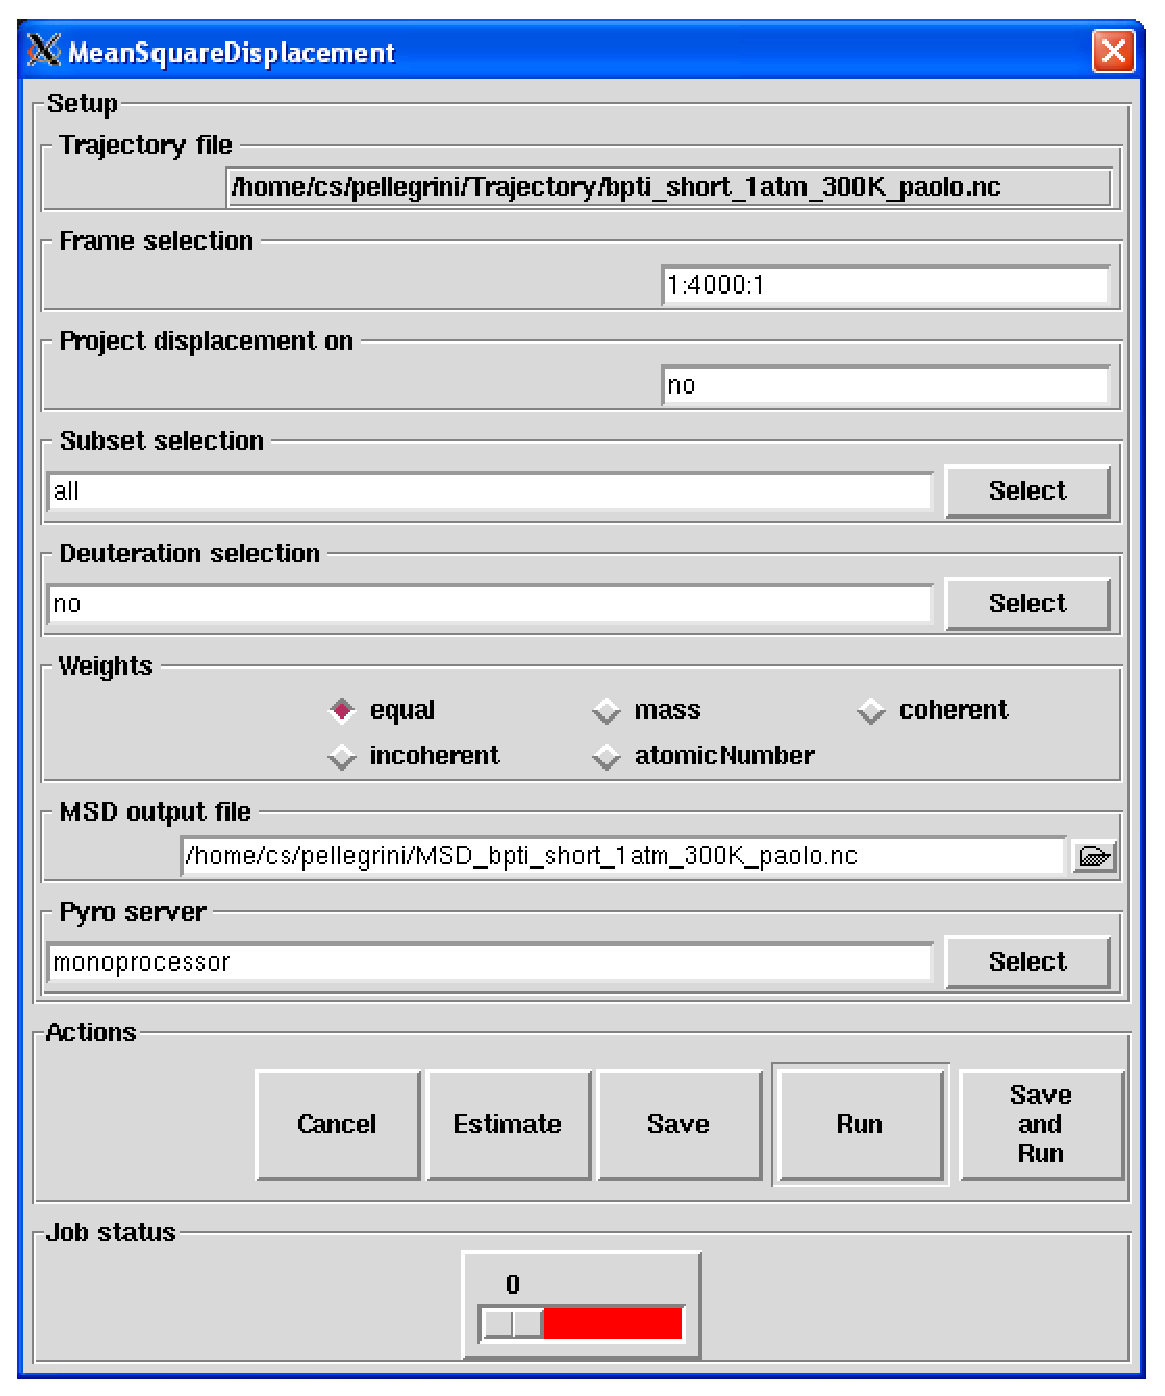
\includegraphics[width=10cm]{Figures/msd.eps}
\end{center}
\caption[The \textit{MSD} analysis dialog]{The dialog from where the \textit{MSD} analysis will be set up and run.}
\label{fig:msd}
\end{figure}   

The following input fields controls the parameters for the \MSD\ analysis:

\begin{itemize}
\item \textbf{Trajectory file}\\
\textbf{Format:} Not an editable entry\\
\textbf{Default:} \textit{traj\_file} where \textit{traj\_file} is the name of the loaded trajectory\\
\textbf{Description:} the value of this widget can not be changed. It just recalls for information purpose the name
of the trajectory file loaded for the analysis.

\item \textbf{Frame selection}\\
\textbf{Format:} string\\
\textbf{Default:} \textit{1:traj\_length:1} where \textit{traj\_length} is the number of frames of the trajectory.\\
\textbf{Description:} this widget allows to select the trajectory frames that will be used for the analysis. This must
be a string of the form:
\\\\
\textit{first:last:step}
\\\\
where \textit{first} is an integer specifying the first frame number to consider, \textit{last} is an integer specifying the last 
frame number to consider and \textit{step} is an integer specifying the step number between two frames.

For example,
\begin{itemize}
\item \textit{2:10:3} will select the frames 2, 5 and 8.
\item \textit{1:5:1} will select the frames 1, 2, 3, 4 and 5.
\end{itemize}

\item \textbf{Project displacement on}\\
\textbf{Format:} string\\
\textbf{Default:} \textit{no}\\
\textbf{Description:} this widget allows to specify a vector along which the \MSD\ will be computed. This vector does not 
need to be normalized as \NMOLDYN\ will perform the normalization when processing it. The entered value must have the 
following format:
\\\\
\textit{vx:vy:vz}
\\\\
where \textit{vx}, \textit{vy} and \textit{vz} are floats that represent respectively the \textit{x}, \textit{y} and \textit{z} coordinates of the vector.

\item \textbf{Subset selection}\\
\textbf{Format:} subset selection string\\
\textbf{Default:} \textit{all}\\
\textbf{Description:} this widget allows the selection of a subset of the system for the analysis. 
See Section \ref{subset_selection} for more details.

\item \textbf{Deuteration selection}\\
\textbf{Format:} deuteration selection string\\
\textbf{Default:} \textit{no}\\
\textbf{Description:} this widget allows the selection of a subset hydrogen atoms that will take the atomic parameters 
of deuterium. See Section \ref{deuteration_selection} for more details.

\item \textbf{Weights}\\
\textbf{Format:} string equal to \textit{equal}, \textit{mass}, \textit{coherent}, \textit{incoherent} or \textit{atomicNumber}\\
\textbf{Default:} \textit{equal}\\
\textbf{Description:} this widget allows the selection of the weighting scheme to apply on each atomic contribution 
to the \MSD . See Section \ref{weighting_scheme} for more details. 

\item \textbf{MSD output file}\\
\textbf{Format:} string\\
\textbf{Default:} \textit{MSD\_traj\_file.nc} where \textit{traj\_file.nc} is the name of the input trajectory\\
\textbf{Description:} this widget allows to enter the name of the \NetCDF\ output file of the \MSD\ analysis. A \CDL\ 
version of the \NetCDF\ output file is also automatically created with \textit{MSD\_traj\_file.cdl} name.
\end{itemize}

\paragraph{Output\\}
The results of a \MSD\ analysis are stored in a \NetCDF\ file whose main variables are namely:
\begin{itemize}
\item time: the times in \ps\ at which the \MSD\ was evaluated,
\item msd: the corresponding \MSD\ in \nmsquare .
\end{itemize}

\subsubsection{Root Mean-Square Deviation}
\label{rmsd}
\paragraph{Theory and implementation\\}
\label{rmsd_theory}
The \RMSD\ is maybe the most popular estimator of structural similarity. It is a 
numerical measure of the difference between two structures that can be defined as:
\begin{equation}
\label{eq:rmsd}
RMSD(t) = \sqrt{\frac{\sum_{\alpha = 1}^{N_{\alpha}}({\bf r}_{\alpha}(t) - {\bf r}_{\alpha}(t_{ref}))}{N_{\alpha}}}
\end{equation}
where $N_{\alpha}$ is the number of atoms of the system, and ${\bf r}_{\alpha}(t)$ and ${\bf r}_{\alpha}(t_{ref})$ are 
respectively the position of atom $\alpha$ at time $t$ and $t_{ref}$ where $t_{ref}$ is a reference time usually 
choosen as the first step of the simulation.
Typically, \RMSD\ is used to quantify the structural evolution of the system during the simulation. It can 
provide precious information about the system especially if it reached equilibrium or conversely if major
structural changes occured during the simulation.

In \NMOLDYN, \RMSD\ is computed using the discretized version of equation \ref{eq:rmsd}:
\begin{equation}
\label{eq:rmsd_num}
RMSD(n\cdot\Delta t) = \sqrt{\frac{\sum_{\alpha = 1}^{N_{\alpha}}({\bf r}_{\alpha}(t) - {\bf r}_{ref}(t))}{N_{\alpha}}},
\qquad n = 0\ldots N_t - 1.
\end{equation}
where $N_t$ is the number of frames and $\Delta t$ is the time step.

\paragraph{Parameters\\}
\label{rmsd_parameters}
Pressing the \textbf{Root Mean-Square Displacement} button will pop up the dialog shown on figure \ref{fig:rmsd}
\begin{figure}[h!]
\begin{center}
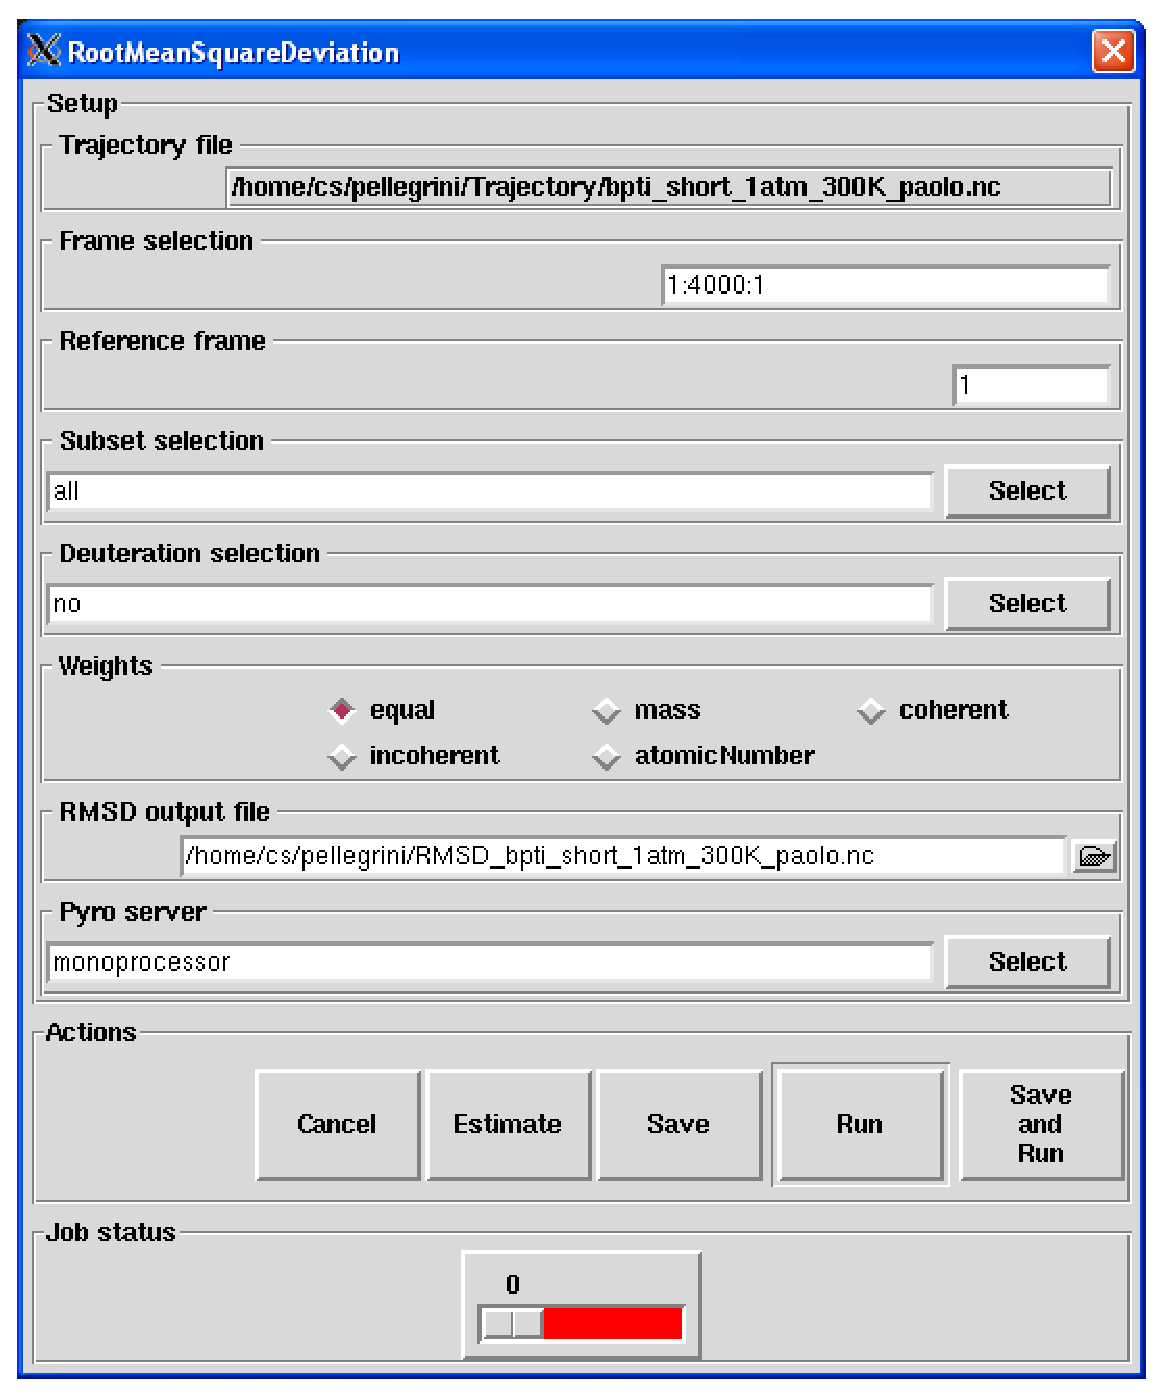
\includegraphics[width=10cm]{Figures/rmsd.eps}
\end{center}
\caption[The \textit{RMSD} analysis dialog]{The dialog from where the \textit{RMSD} analysis will be set up and run.}
\label{fig:rmsd}
\end{figure}   

The following input fields controls the parameters for the \RMSD\ analysis:

\begin{itemize}
\item \textbf{Trajectory file}\\
\textbf{Format:} Not an editable entry\\
\textbf{Default:} \textit{traj\_file} where \textit{traj\_file} is the name of the loaded trajectory\\
\textbf{Description:} the value of this widget can not be changed. It just recalls for information purpose the name
of the trajectory file loaded for the analysis.

\item \textbf{Frame selection}\\
\textbf{Format:} string\\
\textbf{Default:} \textit{1:traj\_length:1} where \textit{traj\_length} is the number of frames of the trajectory.\\
\textbf{Description:} this widget allows to select the trajectory frames that will be used for the analysis. This must
be a string of the form:
\\\\
\textit{first:last:step}
\\\\
where \textit{first} is an integer specifying the first frame number to consider, \textit{last} is an integer specifying the last 
frame number to consider and \textit{step} is an integer specifying the step number between two frames.

For example,
\begin{itemize}
\item \textit{2:10:3} will select the frames 2, 5 and 8.
\item \textit{1:5:1} will select the frames 1, 2, 3, 4 and 5.
\end{itemize}

\item \textbf{Reference frame}\\
\textbf{Format:} integer in [1,\textit{traj\_length}] where \textit{traj\_length} is the number of frames of the input trajectory\\
\textbf{Default:} \textit{1}\\
\textbf{Description:} this widget allows to specify which frame should be the reference for the \RMSD\ analysis.
The value entered should be an integer ranging from 1 to \textit{traj\_length} where \textit{traj\_length} is the 
number of rames of the input trajectory.

\item \textbf{Subset selection}\\
\textbf{Format:} subset selection string\\
\textbf{Default:} \textit{all}\\
\textbf{Description:} this widget allows the selection of a subset of the system for the analysis. 
See Section \ref{subset_selection} for more details.

\item \textbf{Deuteration selection}\\
\textbf{Format:} deuteration selection string\\
\textbf{Default:} \textit{no}\\
\textbf{Description:} this widget allows the selection of a subset hydrogen atoms that will take the atomic parameters 
of deuterium. See Section \ref{deuteration_selection} for more details.

\item \textbf{Weights}\\
\textbf{Format:} string equal to \textit{equal}, \textit{mass}, \textit{coherent}, \textit{incoherent} or \textit{atomicNumber}\\
\textbf{Default:} \textit{equal}\\
\textbf{Description:} this widget allows the selection of the weighting scheme to apply on each atomic contribution 
to the \RMSD . See Section \ref{weighting_scheme} for more details. 

\item \textbf{RMSD output file}\\
\textbf{Format:} string\\
\textbf{Default:} \textit{RMSD\_traj\_file.nc} where \textit{traj\_file.nc} is the name of the input trajectory\\
\textbf{Description:} this widget allows to enter the name of the \NetCDF\ output file of the \RMSD\ analysis. A \CDL\ 
version of the \NetCDF\ output file is also automatically created with \textit{RMSD\_traj\_file.cdl} name.
\end{itemize}

\paragraph{Output\\}
The results of a \RMSD\ analysis are stored in a \NetCDF\ file whose main variables are namely:
\begin{itemize}
\item time: the times in \ps\ at which the \RMSD\ was evaluated,
\item rmsd: the corresponding \RMSD\ in \nm .
\end{itemize}

\subsubsection{Radius of gyration}
\label{rog}
\paragraph{Theory and implementation\\}
\label{rog_theory}
\ROG\ is the name of several related measures of the size of an object, a surface, or an ensemble of 
points. It is calculated as the Root Mean Square Distance between the system and a reference that can be either 
the center of gravity of the system either a given axis. In \NMOLDYN, the reference is choosen to be the center 
of gravity of the system under study. Mathematically, it can be defined as:
\begin{equation}
\label{eq:rog}
ROG(t) = \sqrt{\frac{\sum_{\alpha = 1}^{N_{\alpha}}({\bf r}_{\alpha}(t) - {\bf r}_{cms}(t))}{N_{\alpha}}}
\end{equation}
where $N_{\alpha}$ is the number of atoms of the system, and ${\bf r}_{\alpha}(t)$ and ${\bf r}_{cms}(t)$ are 
respectively the position of atom $\alpha$ and the center of mass of the system at time $t$.

\ROG\ describes the overall spread of the molecule and as such is a good measure for the molecule compactness. For
example, it can be useful when monitoring folding process.

In \NMOLDYN, \ROG\ is computed using the discretized version of equation \ref{eq:rog}:
\begin{equation}
\label{eq:rog_num}
ROG(n\cdot\Delta t) = \sqrt{\frac{\sum_{\alpha = 1}^{N_{\alpha}}({\bf r}_{\alpha}(t) - {\bf r}_{cms}(t))}{N_{\alpha}}},
\qquad n = 0\ldots N_t - 1.
\end{equation}
where $N_t$ is the number of frames and $\Delta t$ is the time step.
\newpage
\paragraph{Parameters\\}
\label{rog_parameters}
Pressing the \textbf{Radius Of Gyration} button will pop up the dialog shown on figure \ref{fig:rog}
\begin{figure}[h!]
\begin{center}
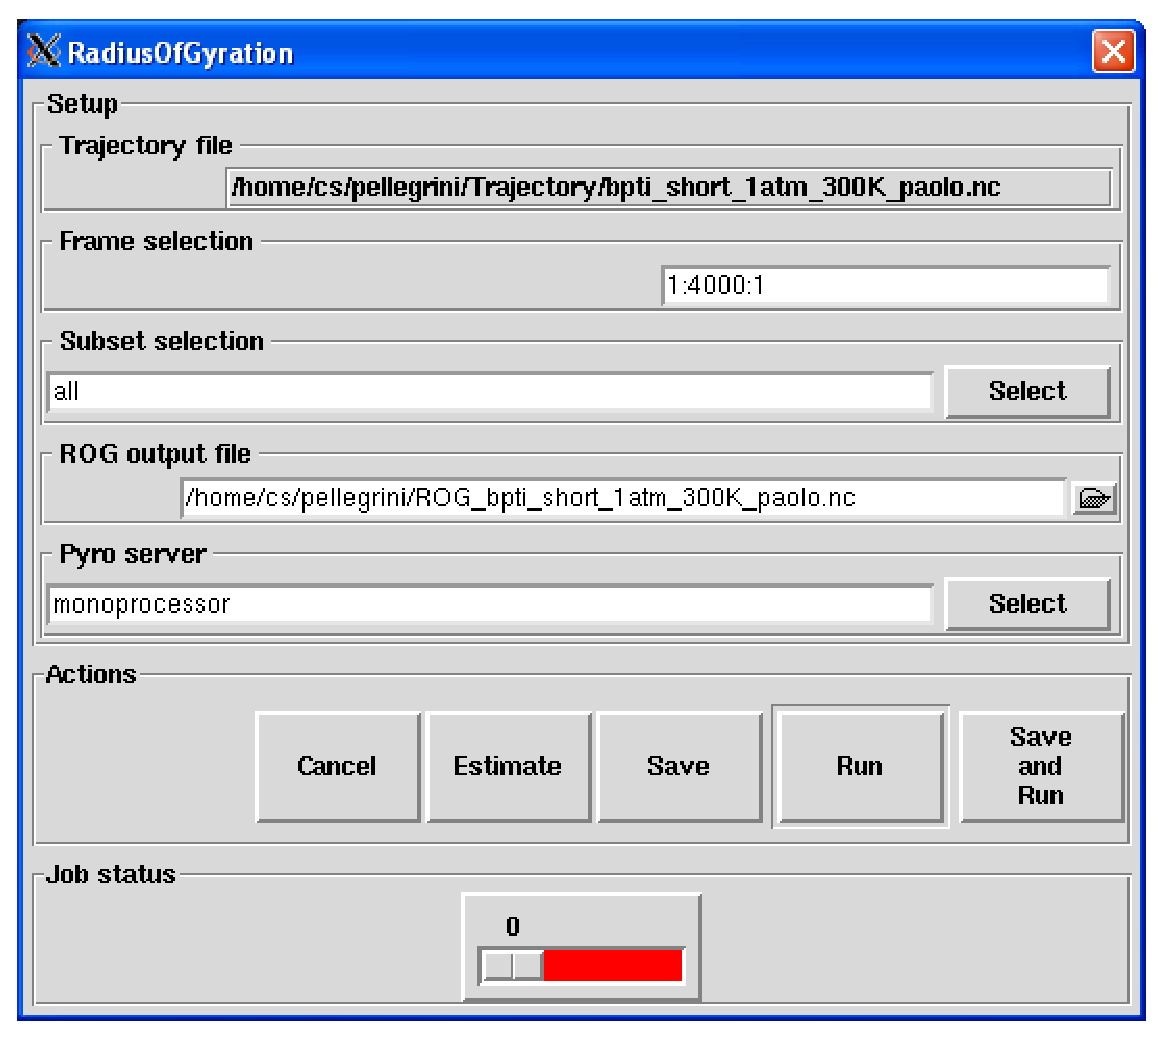
\includegraphics[width=10cm]{Figures/rog.eps}
\end{center}
\caption[The \textit{ROG} analysis dialog]{The dialog from where the \textit{ROG} analysis will be set up and run.}
\label{fig:rog}
\end{figure}   

The following input fields controls the parameters for the \ROG\ analysis:

\begin{itemize}
\item \textbf{Trajectory file}\\
\textbf{Format:} Not an editable entry\\
\textbf{Default:} \textit{traj\_file} where \textit{traj\_file} is the name of the loaded trajectory\\
\textbf{Description:} the value of this widget can not be changed. It just recalls for information purpose the name
of the trajectory file loaded for the analysis.

\item \textbf{Frame selection}\\
\textbf{Format:} string\\
\textbf{Default:} \textit{1:traj\_length:1} where \textit{traj\_length} is the number of frames of the trajectory.\\
\textbf{Description:} this widget allows to select the trajectory frames that will be used for the analysis. This must
be a string of the form:
\\\\
\textit{first:last:step}
\\\\
where \textit{first} is an integer specifying the first frame number to consider, \textit{last} is an integer specifying the last 
frame number to consider and \textit{step} is an integer specifying the step number between two frames.

For example,
\begin{itemize}
\item \textit{2:10:3} will select the frames 2, 5 and 8.
\item \textit{1:5:1} will select the frames 1, 2, 3, 4 and 5.
\end{itemize}

\item \textbf{Subset selection}\\
\textbf{Format:} subset selection string\\
\textbf{Default:} \textit{all}\\
\textbf{Description:} this widget allows the selection of a subset of the system for the analysis. 
See Section \ref{subset_selection} for more details.

\item \textbf{Deuteration selection}\\
\textbf{Format:} deuteration selection string\\
\textbf{Default:} \textit{no}\\
\textbf{Description:} this widget allows the selection of a subset hydrogen atoms that will take the atomic parameters 
of deuterium. See Section \ref{deuteration_selection} for more details.

\item \textbf{Weights}\\
\textbf{Format:} string equal to \textit{equal}, \textit{mass}, \textit{coherent}, \textit{incoherent} or \textit{atomicNumber}\\
\textbf{Default:} \textit{equal}\\
\textbf{Description:} this widget allows the selection of the weighting scheme to apply on each atomic contribution 
to the \ROG. See Section \ref{weighting_scheme} for more details. 

\item \textbf{ROG output file}\\
\textbf{Format:} string\\
\textbf{Default:} \textit{ROG\_traj\_file.nc} where \textit{traj\_file.nc} is the name of the input trajectory\\
\textbf{Description:} this widget allows to enter the name of the \NetCDF\ output file of the \ROG\ analysis. A \CDL\ 
version of the \NetCDF\ output file is also automatically created with \textit{ROG\_traj\_file.cdl} name.
\end{itemize}

\paragraph{Output\\}
The results of a \ROG\ analysis are stored in a \NetCDF\ file whose main variables are namely:
\begin{itemize}
\item time: the times in \ps\ at which the \ROG\ was evaluated,
\item rog: the corresponding \ROG\ in \nm .
\end{itemize}

\subsubsection{Angular Correlation}
\label{ac}
\paragraph{Theory and implementation\\}
\label{ac_theory}
The angular correlation analysis computes the autocorrelation of a set of vectors describing the extent of a molecule in three 
orthogonal directions. This kind of analysis can be useful when trying to highlight the fact that a molecule is constrainted 
in a given direction.

For a given triplet of non-colinear atoms \textit{g}=(\textbf{a1},\textbf{a2},\textbf{a3}), one can derive an orthonormal 
set of three vectors ${\bf v}_1$, ${\bf v}_2$, ${\bf v}_3$ using the following scheme:

\begin{itemize}
\item ${\bf v}_1 = \frac{{\bf n}_{1} + {\bf n}_{2}}{||{\bf n}_{1} + {\bf n}_{2}||}$
where ${\bf n}_{1}$ and ${\bf n}_{2}$ are respectively the normalized vectors along (\textbf{a1},\textbf{a2}) 
and (\textbf{a1},\textbf{a3}) directions.
\item ${\bf v}_2$ is defined as the clockwise normal vector orthogonal to ${\bf v}_1$ that belongs to the plane 
defined by \textbf{a1}, \textbf{a2} and \textbf{a3} atoms
\item $\vec{v_3} = \vec{v_1} \times \vec{v_2}$
\end{itemize}

Thus, one can define the following autocorrelation functions for the vectors ${\bf v}_1$, ${\bf v}_2$ and ${\bf v}_3$ 
defined on triplet \textit{t}:
\begin{equation}
\label{eq:ac_per_triplet}
AC_{g,i} (t) = \langle {\bf v}_{t,i}(0)\cdot{\bf v}_{t,i}(t)\rangle, \qquad  i = 1,2,3
\end{equation}

And the angular correlation averaged over all triplets is:
\begin{equation}
\label{eq:ac}
AC_i(t) = \sum_{g=1}^{N_{triplets}} AC_{g,i}(t), \qquad  i = 1,2,3
\end{equation}
where $N_{triplets}$ is the number of selected triplets.

\paragraph{Parameters\\}
\label{ac_parameters}
Pressing the \textbf{Angular Correlation} button will pop up the dialog shown on figure \ref{fig:ac}
\begin{figure}[h!]
\begin{center}
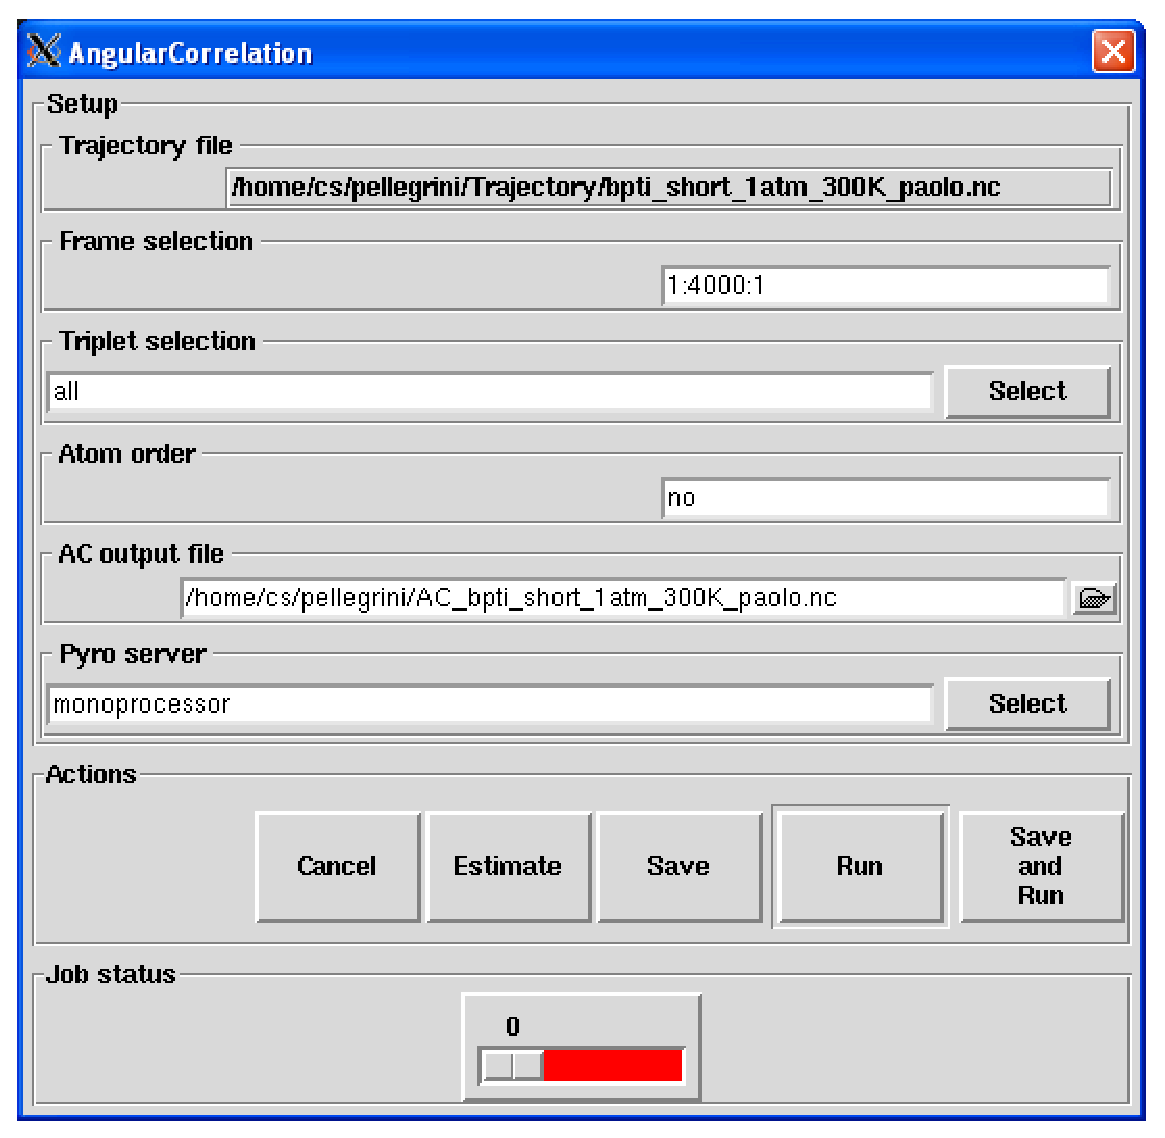
\includegraphics[width=10cm]{Figures/ac.eps}
\end{center}
\caption[The \textit{AC} analysis dialog]{The dialog from where the \textit{AC} analysis will be set up and run.}
\label{fig:ac}
\end{figure}   

The following input fields controls the parameters for the \AC\ analysis:

\begin{itemize}
\item \textbf{Trajectory file}\\
\textbf{Format:} string\\
\textbf{Default:} \textit{traj\_file} where \textit{traj\_file} is the name of the loaded trajectory\\
\textbf{Description:} the value of this widget can not be changed. It just recalls for information purpose the name
of the trajectory file loaded for the analysis.

\item \textbf{Frame selection}\\
\textbf{Format:} string\\
\textbf{Default:} \textit{1:traj\_length:1} where \textit{traj\_length} is the number of frames of the trajectory.\\
\textbf{Description:} this widget allows to select the trajectory frames that will be used for the analysis. This must
be a string of the form:
\\\\
\textit{first:last:step}
\\\\
where \textit{first} is an integer specifying the first frame number to consider, \textit{last} is an integer specifying the last 
frame number to consider and \textit{step} is an integer specifying the step number between two frames.

For example,
\begin{itemize}
\item \textit{2:10:3} will select the frames 2, 5 and 8.
\item \textit{1:5:1} will select the frames 1, 2, 3, 4 and 5.
\end{itemize}

\item \textbf{Triplet selection}\\
\textbf{Format:} group selection string\\
\textbf{Default:} \textit{all}\\
\textbf{Description:} this widget allows the selection of the triplets of atoms from which the analysis will be 
performed. See Section \ref{group_selection} for more details. Any selection that does not contain exactly three atoms will 
be discarded.

\item \textbf{Atom order}\\
\textbf{Format:} string\\
\textbf{Default:} \textit{no}\\
\textbf{Description:} this widget allows to specify the order in which the atoms \textbf{a1}, \textbf{a2} and \textbf{a3} should be 
ordered. By default, the order will be defined by \NMOLDYN\ by ranking for the atoms of each triplet by their
\MMTK\ name. Otherwise, the entered value must have the following specific format:
\\\\
\textit{\MMTK\ name for \textbf{a1},\MMTK\ name for \textbf{a2},\MMTK\ name for \textbf{a3}}

\item \textbf{AC output file}\\
\textbf{Format:} string\\
\textbf{Default:} \textit{AC\_traj\_file.nc} where \textit{traj\_file.nc} is the name of the input trajectory\\
\textbf{Description:} this widget allows to enter the name of the \NetCDF\ output file of the \AC\ analysis. A \CDL\ 
version of the \NetCDF\ output file is also automatically created with \textit{AC\_traj\_file.cdl} name.
\end{itemize}
\newpage
\paragraph{Output\\}
The results of a \AC\ analysis are stored in a \NetCDF\ file whose main variables are namely:
\begin{itemize}
\item time: the times in \ps\ at which the \AC\ was evaluated,
\item triplet: the index for each triplet considered in the analysis,
\item ac\_1\_by\_triplet: the angular correlation of ${\bf v}_1$ for each triplet according Eq.\ref{eq:ac_per_triplet},
\item ac\_2\_by\_triplet: the angular correlation of ${\bf v}_2$ for each triplet according Eq.\ref{eq:ac_per_triplet},
\item ac\_3\_by\_triplet: the angular correlation of ${\bf v}_3$ for each triplet according Eq.\ref{eq:ac_per_triplet},
\item ac\_1: the group-averaged angular correlation for ${\bf v}_1$ according Eq.\ref{eq:ac},
\item ac\_2: the group-averaged angular correlation for ${\bf v}_2$ according Eq.\ref{eq:ac},
\item ac\_3: the group-averaged angular correlation for ${\bf v}_3$ according Eq.\ref{eq:ac}.
\end{itemize}

\subsubsection{Velocity Autocorrelation Function}
\label{vacf}
\paragraph{Theory and implementation\\}
\label{vacf_theory}
The \VACF\ is another interesting property describing the dynamics of a 
molecular system. Indeed, it reveals the underlying nature of the forces acting on the system. 

In a molecular system that would be made of non interacting particles, the velocities would be constant at 
any time triggering the \VACF\ to be a constant value. Now, if we think about a system with small interactions such as in a
gas-phase, the magnitude and direction of the velocity of a particle will change gradually over time due to its 
collision with the other particles of the molecular system. In such a system, the \VACF\ will be represented by a
decaying exponential.

In the case of solid phase, the interaction are much stronger and, as a results, the atoms are bound to a given 
position from which they will move backwards and forwards oscillating between positive and negative values of 
their velocity. The oscillations will not be of equal magnitude however, but will decay in time, because there 
are still perturbative forces acting on the atoms to disrupt the perfection of their oscillatory motion. So, in 
that case the \VACF\ will look like a damped harmonic motion.

Finally, in the case of liquid phase, the atoms have more freedom than in solid phase and because of the diffusion 
process, the oscillatory motion seen in solid phase will be cancelled quite rapidly depending on the density of the
system. So, the \VACF\ will just have one very damped oscillation before decaying to zero. This decaying time can be
considered as the average time for a collision between two atoms to occur before they diffuse away.

Mathematically, the \VACF\ of atom $\alpha$ in an atomic or molecular system is usually defined as
\begin{equation}
\label{eq:vacf}
C_{vv ; \alpha\alpha}(t) \doteq
\frac{1}{3}\langle {\bf v}_\alpha(t_0)\cdot{\bf v}_\alpha(t_0+t)\rangle_{t_0}.
\end{equation}
In some cases, e.g. for non-isotropic systems, it is useful to define \VACF\ along a given axis,
\begin{equation}
\label{eq:vacf_n}
C_{vv ; \alpha\alpha}(t;{\bf n}) \doteq
\langle v_\alpha(t_0;{\bf n})v_\alpha(t_0+t;{\bf n})\rangle_{t_0},
\end{equation}
where $v_\alpha(t;{\bf n})$ is given by
\begin{equation}
v_\alpha(t;{\bf n}) \doteq 
{\bf n}\cdot{\bf v}_{\alpha}(t).
\end{equation}
The vector \textit{\textbf{n}} is a unit vector defining a space-fixed axis.

The \VACF\ of the particles in a many body system can be related to the
incoherent dynamic structure factor by the relation:
\begin{equation}
\label{eq:sqw_dos}
lim_{q\to 0} \frac{\omega^2}{q^2}{\cal S}({\bf q},\omega) =
G(\omega), 
\end{equation}
where $G(\omega)$ is the \DOS. For an isotropic system it reads
\begin{eqnarray}
\label{eq:dos}
G(\omega) &= &\sum_{\alpha}b^2_{\alpha,inc}
\tilde C_{vv ; \alpha\alpha}(\omega),\\
\label{eq:dos_alpha}
\tilde C_{vv ; \alpha\alpha}(\omega) &= &
\frac{1}{2\pi}\int_{-\infty}^{+\infty}dt\, \exp[-i\omega t] 
C_{vv ; \alpha\alpha}(t).
\end{eqnarray}
For non-isotropic systems relation (\ref{eq:sqw_dos}) holds if the \DOS\ is computed from the atomic velocity 
autocorrelation functions $C_{vv ; \alpha\alpha}(t;{\bf n}_q)$, where ${\bf n}_q$ is the unit vector in the 
direction of \textit{\textbf{q}}.

\paragraph{Parameters\\}
\label{vacf_parameters}
Pressing the \textbf{Velocity Autocorrelation Function} button will pop up the dialog shown on figure \ref{fig:vacf}
\begin{figure}[h!]
\begin{center}
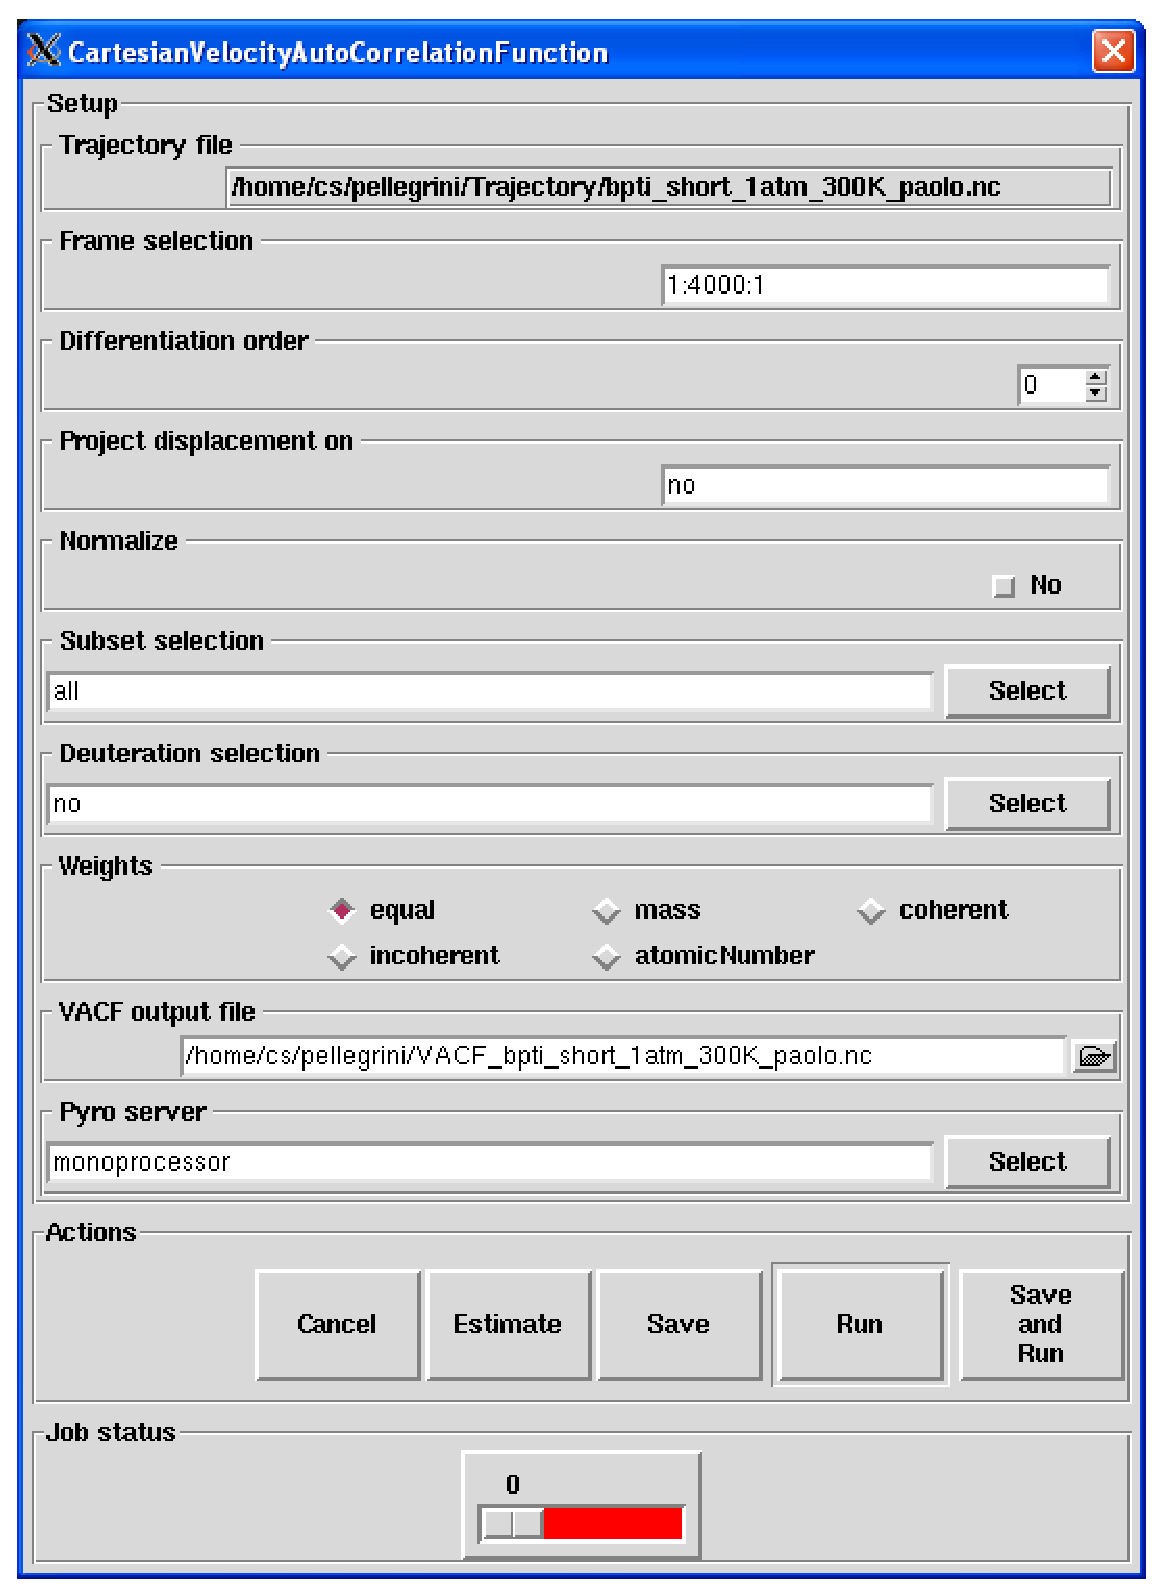
\includegraphics[width=10cm]{Figures/vacf.eps}
\end{center}
\caption[The \textit{VACF} analysis dialog]{The dialog from where the \textit{VACF} analysis will be set up and run.}
\label{fig:vacf}
\end{figure}   

The following input fields controls the parameters for the \VACF\ analysis:

\begin{itemize}
\item \textbf{Trajectory file}\\
\textbf{Format:} string\\
\textbf{Default:} \textit{traj\_file} where \textit{traj\_file} is the name of the loaded trajectory\\
\textbf{Description:} the value of this widget can not be changed. It just recalls for information purpose the name
of the trajectory file loaded for the analysis.

\item \textbf{Frame selection}\\
\textbf{Format:} string\\
\textbf{Default:} \textit{1:traj\_length:1} where \textit{traj\_length} is the number of frames of the trajectory.\\
\textbf{Description:} this widget allows to select the trajectory frames that will be used for the analysis. This must
be a string of the form:
\\\\
\textit{first:last:step}
\\\\
where \textit{first} is an integer specifying the first frame number to consider, \textit{last} is an integer specifying the last 
frame number to consider and \textit{step} is an integer specifying the step number between two frames.

For example,
\begin{itemize}
\item \textit{2:10:3} will select the frames 2, 5 and 8.
\item \textit{1:5:1} will select the frames 1, 2, 3, 4 and 5.
\end{itemize}

\item \textbf{Differentiation order}\\
\textbf{Format:} integer in [0,5]\\
\textbf{Default:} 0 if velocities are stored in the trajectory file, 1 otherwise\\
\textbf{Description:} this widget allows to specify the order of the derivation scheme used to get the velocities out 
of the coordinates. If your trajectory \NetCDF\ file already contains the velocities then just select \textit{0}.
However, you can still decide to get the velocities out of the coordinates. In that case, \NMOLDYN\ performs a numerical 
differentiation of the input data. To do so, \NMOLDYN\ can perform numerical differentiation from order \textit{1} to 
order \textit{5}. Using order \textit{1}, the first time derivative of each point $r(t_i)$ 
is calculated as
\begin{equation}
\dot{r}(t_i)=\frac{r(t_{i+1})-r(t_{i})} {\Delta t},
\end{equation}
where $\Delta t$ is the time step. 
Choosing order \textit{N} with \textit{N=2,...,5}, \NMOLDYN\ calculates the first time-derivative of each point 
$r(t_i)$ ($r=x,y,z$) using the \textit{N}-order polynomial interpolating the \textit{N+1} points across $r(t_i)$, where $r(t_i)$ 
belongs to this set \cite{Abramowitz}.
\newpage
\item \textbf{Project displacement on}\\
\textbf{Format:} string\\
\textbf{Default:} \textit{no}\\
\textbf{Description:} this widget allows to specify a vector along which the \VACF\ will be computed. This vector does not 
need to be normalized as \NMOLDYN\ will perform the normalization when processing it. The entered value must have the 
following format:
\\\\
\textit{vx:vy:vz}
\\\\
where \textit{vx}, \textit{vy} and \textit{vz} are floats that represent respectively the \textit{x}, \textit{y} and \textit{z} coordinates of the vector.

\item \textbf{Normalize}\\
\textbf{Format:} string equal to \textit{yes} or \textit{no}\\
\textbf{Default:} \textit{no}\\
\textbf{Description:} if set to \textit{yes} normalize to 1 the \textit{VACF(t = 0)}.

\item \textbf{Subset selection}\\
\textbf{Format:} subset selection string\\
\textbf{Default:} \textit{all}\\
\textbf{Description:} this widget allows the selection of a subset of the system for the analysis. 
See Section \ref{subset_selection} for more details.

\item \textbf{Deuteration selection}\\
\textbf{Format:} deuteration selection string\\
\textbf{Default:} \textit{no}\\
\textbf{Description:} this widget allows the selection of a subset hydrogen atoms that will take the atomic parameters 
of deuterium. See Section \ref{deuteration_selection} for more details.

\item \textbf{Weights}\\
\textbf{Format:} string equal to \textit{equal}, \textit{mass}, \textit{coherent}, \textit{incoherent} or \textit{atomicNumber}\\
\textbf{Default:} \textit{equal}\\
\textbf{Description:} this widget allows the selection of the weighting scheme to apply on each atomic contribution 
to the \VACF. See Section \ref{weighting_scheme} for more details. 

\item \textbf{VACF output file}\\
\textbf{Format:} string\\
\textbf{Default:} \textit{VACF\_traj\_file.nc} where \textit{traj\_file.nc} is the name of the input trajectory\\
\textbf{Description:} this widget allows to enter the name of the \NetCDF\ output file of the \VACF\ analysis. A \CDL\ 
version of the \NetCDF\ output file is also automatically created with \textit{VACF\_traj\_file.cdl} name.
\end{itemize}

\paragraph{Output\\}
The results of a \VACF\ analysis are stored in a \NetCDF\ file whose main variables are namely:
\begin{itemize}
\item time: the times in \ps\ at which the \VACF\ was evaluated,
\item vacf: the corresponding \VACF\ in \vacfunits .
\end{itemize}

\subsubsection{Density Of States}
\label{dos}
\paragraph{Theory and implementation\\}
\label{dos_theory}
\NMOLDYN\ calculates the power spectrum of the \VACF, which in case of the mass-weighted \VACF\ defines the phonon 
discrete \DOS, (see Section \ref{vacf_theory}) defined as:
\begin{eqnarray}
DOS(n\cdot\Delta \nu)  &\doteq &\sum_{\alpha} \omega_\alpha 
\tilde C_{vv ; \alpha\alpha}(n\cdot\Delta \nu),\qquad n = 0\ldots N_t - 1.
\end{eqnarray}
$N_t$ is the total number of time steps and $\Delta\nu = 1/(2N_t \Delta t)$ is the frequency step. $DOS(n\cdot\Delta\nu)$ can 
be computed either for the isotropic case or with respect to a user-defined axis. The spectrum $DOS(n\cdot\Delta \nu)$ is computed from the 
\textit{unnormalized} \VACF, such that \textit{DOS(0)} gives an approximate value for the diffusion constant 
$D = \sum_\alpha D_\alpha$ (see Eqs. \ref{eq:d_vacf} and \ref{eq:d_dos}). $DOS(n\cdot\Delta \nu)$ is smoothed by 
applying a Gaussian window in the time domain \cite{Harris} (see Section \ref{fca}). Its width in the time domain is 
$\sigma_t=\alpha/T$, where $T$ is the length of 
the simulation. We remark that the diffusion constant obtained from \DOS\ is biased due to the spectral smoothing procedure since 
the \VACF\ is weighted by this window Gaussian function. \NMOLDYN\ computes the density of states starting from both atomic velocities 
and atomic coordinates. In this case the velocities are computed by numerical differentiation of the coordinate trajectories correcting 
first for possible jumps due to periodic boundary conditions.

\paragraph{Parameters\\}
\label{dos_parameters}
Pressing the \textbf{Density Of States} button will pop up the dialog shown on figure \ref{fig:dos}
\begin{figure}[h!]
\begin{center}
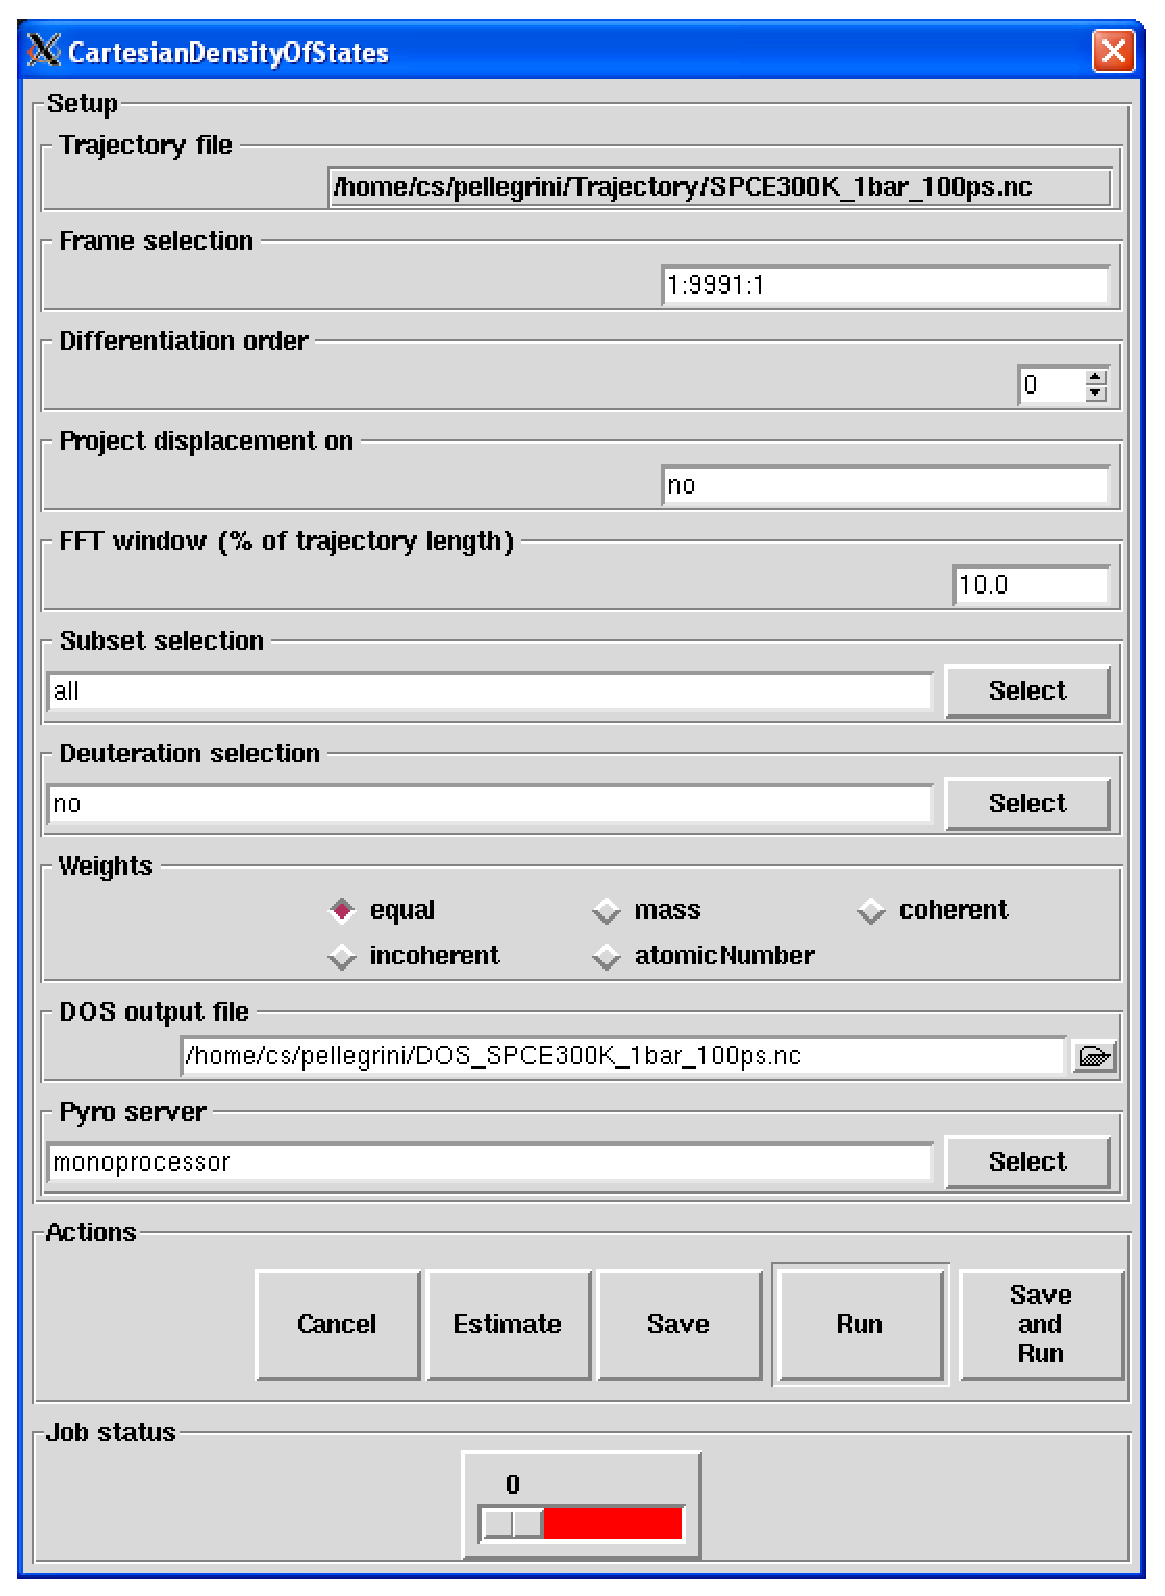
\includegraphics[width=10cm]{Figures/dos.eps}
\end{center}
\caption[The \textit{DOS} analysis dialog]{The dialog from where the \textit{DOS} analysis will be set up and run.}
\label{fig:dos}
\end{figure}   

The following input fields controls the parameters for the \DOS\ analysis:

\begin{itemize}
\item \textbf{Trajectory file}\\
\textbf{Format:} string\\
\textbf{Default:} \textit{traj\_file} where \textit{traj\_file} is the name of the loaded trajectory\\
\textbf{Description:} the value of this widget can not be changed. It just recalls for information purpose the name
of the trajectory file loaded for the analysis.

\item \textbf{Frame selection}\\
\textbf{Format:} string\\
\textbf{Default:} \textit{1:traj\_length:1} where \textit{traj\_length} is the number of frames of the trajectory.\\
\textbf{Description:} this widget allows to select the trajectory frames that will be used for the analysis. This must
be a string of the form:
\\\\
\textit{first:last:step}
\\\\
where \textit{first} is an integer specifying the first frame number to consider, \textit{last} is an integer specifying the last 
frame number to consider and \textit{step} is an integer specifying the step number between two frames.

For example,
\begin{itemize}
\item \textit{2:10:3} will select the frames 2, 5 and 8.
\item \textit{1:5:1} will select the frames 1, 2, 3, 4 and 5.
\end{itemize}

\item \textbf{Differentiation order}\\
\textbf{Format:} integer in [0,5]\\
\textbf{Default:} 0 if velocities are stored in the trajectory file, 1 otherwise\\
\textbf{Description:} this widget allows to specify the order of the derivation scheme used to get the velocities out 
of the coordinates. If your trajectory \NetCDF\ file already contains the velocities then just select \textit{0}.
However, you can still decide to get the velocities out of the coordinates. In that case, \NMOLDYN\ performs a numerical 
differentiation of the input data. To do so, \NMOLDYN\ can perform numerical differentiation from order \textit{1} to 
order \textit{5}. Using order \textit{1}, the first time derivative of each point $r(t_i)$ 
is calculated as
\begin{equation}
\dot{r}(t_i)=\frac{r(t_{i+1})-r(t_{i})} {\Delta t},
\end{equation}
where $\Delta t$ is the time step. 
Choosing order \textit{N} with \textit{N=2,...,5}, \NMOLDYN\ calculates the first time-derivative of each point 
$r(t_i)$ ($r=x,y,z$) using the \textit{N}-order polynomial interpolating the \textit{N+1} points across $r(t_i)$, where $r(t_i)$ 
belongs to this set \cite{Abramowitz}.

\item \textbf{Project displacement on}\\
\textbf{Format:} string\\
\textbf{Default:} \textit{no}\\
\textbf{Description:} this widget allows to specify a vector along which the \DOS\ will be computed. This vector does not 
need to be normalized as \NMOLDYN\ will perform the normalization when processing it. The entered value must have the 
following format:
\\\\
\textit{vx:vy:vz}
\\\\
where \textit{vx}, \textit{vy} and \textit{vz} are floats that represent respectively the \textit{x}, \textit{y} and \textit{z} coordinates of the vector.

\item \textbf{FFT window}\\
\textbf{Format:} float in [0.0,100.0]\\
\textbf{Default:} \textit{10.0}\\
\textbf{Description:} this widget allows to define the width in percentage of the trajectory length of the Gaussian 
function to be used in the smoothing procedure for the calculation of the \DOS. See Appendix \ref{fca} for more details.

\item \textbf{Subset selection}\\
\textbf{Format:} subset selection string\\
\textbf{Default:} \textit{all}\\
\textbf{Description:} this widget allows the selection of a subset of the system for the analysis. 
See Section \ref{subset_selection} for more details.

\item \textbf{Deuteration selection}\\
\textbf{Format:} deuteration selection string\\
\textbf{Default:} \textit{no}\\
\textbf{Description:} this widget allows the selection of a subset hydrogen atoms that will take the atomic parameters 
of deuterium. See Section \ref{deuteration_selection} for more details.

\item \textbf{Weights}\\
\textbf{Format:} string equal to \textit{equal}, \textit{mass}, \textit{coherent}, \textit{incoherent} or \textit{atomicNumber}\\
\textbf{Default:} \textit{equal}\\
\textbf{Description:} this widget allows the selection of the weighting scheme to apply on each atomic contribution 
to the \DOS. See Section \ref{weighting_scheme} for more details. 

\item \textbf{DOS Output file}\\
\textbf{Format:} string\\
\textbf{Default:} \textit{DOS\_traj\_file.nc} where \textit{traj\_file.nc} is the name of the input trajectory\\
\textbf{Description:} this widget allows to enter the name of the \NetCDF\ output file of the \DOS\ analysis. A \CDL\ 
version of the \NetCDF\ output file is also automatically created with \textit{DOS\_traj\_file.cdl} name.
\end{itemize}

\paragraph{Output\\}
The results of a \DOS\ analysis are stored in a \NetCDF\ file whose main variables are namely:
\begin{itemize}
\item frequency: the frequencies in \thz\ at which the \DOS\ was evaluated,
\item dos: the corresponding \DOS .
\end{itemize}

\subsubsection{Pass-Band Filtered Trajectory}
\label{pbft}
\paragraph{Theory and implementation\\}
\label{pbft_theory}
It is often of interest to restrict attention to motions in a specific frequency interval, both for quantitative analysis 
and for visualization by animated display. This is particularly useful to study low-frequency motions without being 
distracted by the high frequency "noise". \NMOLDYN\ can create \PBFT\ by applying a frequency pass-band filter to the 
atomic trajectories, either on the whole system or on an user-defined subset. The result is stored in a new trajectory file that contains only motions in the 
chosen interval. Frequency filtering uses a straightforward algorithm:
\begin{itemize}
\item take the discrete Fourier transform of each particle trajectory,
\item set the Fourier coefficients outside the filtering interval to zero,
\item and transform back to the time domain.
\end{itemize} 
This corresponds to applying a rectangular window in the frequency domain.

\paragraph{Parameters\\}
\label{pbft_parameters}
Pressing the \textbf{Pass-Band Filtered Trajectory} button will pop up the dialog shown on figure \ref{fig:pbft}
\begin{figure}[h!]
\begin{center}
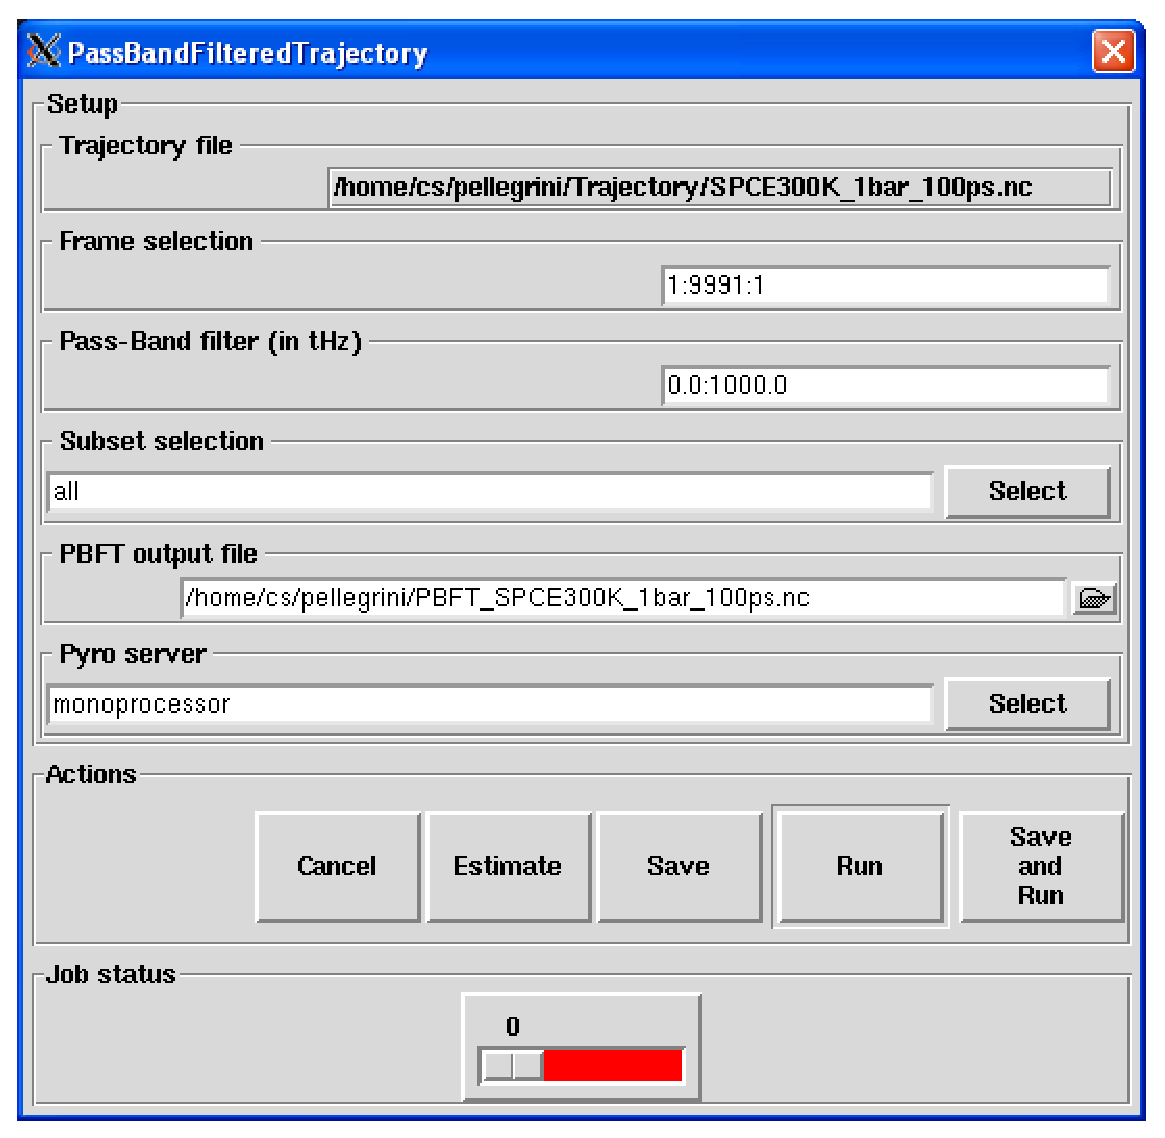
\includegraphics[width=10cm]{Figures/pbft.eps}
\end{center}
\caption[The \textit{PBFT} analysis dialog]{The dialog from where the \textit{PBFT} analysis will be set up and run.}
\label{fig:pbft}
\end{figure}   

The following input fields controls the parameters for the \PBFT\ analysis:

\begin{itemize}
\item \textbf{Trajectory file}\\
\textbf{Format:} string\\
\textbf{Default:} \textit{traj\_file} where \textit{traj\_file} is the name of the loaded trajectory\\
\textbf{Description:} the value of this widget can not be changed. It just recalls for information purpose the name
of the trajectory file loaded for the analysis.

\item \textbf{Frame selection}\\
\textbf{Format:} string\\
\textbf{Default:} \textit{1:traj\_length:1} where \textit{traj\_length} is the number of frames of the trajectory.\\
\textbf{Description:} this widget allows to select the trajectory frames that will be used for the analysis. This must
be a string of the form:
\\\\
\textit{first:last:step}
\\\\
where \textit{first} is an integer specifying the first frame number to consider, \textit{last} is an integer specifying the last 
frame number to consider and \textit{step} is an integer specifying the step number between two frames.

For example,
\begin{itemize}
\item \textit{2:10:3} will select the frames 2, 5 and 8.
\item \textit{1:5:1} will select the frames 1, 2, 3, 4 and 5.
\end{itemize}

\item \textbf{Pass-band filter}\\
\textbf{Format:} string\\
\textbf{Default:} \textit{0.0:1000.0}\\
\textbf{Description:} this widget allows to specify respectively the minimum and maximum frequencies for the pass-band filter. 
The entered value must have the following format:
\\\\
\textit{fmin:fmax}
\\\\
where \textit{fmin} and \textit{fmax} are respectively the minimum and maximum frequencies in \thz\ of the pass-band filter.
\newpage
\item \textbf{Subset selection}\\
\textbf{Format:} subset selection string\\
\textbf{Default:} \textit{all}\\
\textbf{Description:} this widget allows the selection of a subset of the system for the analysis. 
See Section \ref{subset_selection} for more details.

\item \textbf{PBFT Output file}\\
\textbf{Format:} string\\
\textbf{Default:} \textit{PBFT\_traj\_file.nc} where \textit{traj\_file.nc} is the name of the input trajectory\\
\textbf{Description:} this widget allows to enter the name of the \NetCDF\ output file of the \PBFT\ analysis.
\end{itemize}

\paragraph{Output\\}
The results of a \PBFT\ analysis is a \MMTK\ \NetCDF\ trajectory file containing the pass-band filtered trajectory.

\subsubsection{Global Motion Filtered Trajectory}
\label{gmft}
\paragraph{Theory and implementation\\}
\label{gmft_theory}
It is often of interest to separate global motion from internal motion, both for quantitative analysis 
and for visualization by animated display. Obviously, this can be done under the hypothesis that global and internal 
motions are decoupled within the length and timescales of the analysis. \NMOLDYN\ can create \GMFT\ by filtering out global 
motions (made of the three translational and rotational degrees of freedom), either on the whole system or on an user-defined subset, 
by fitting it to a reference structure (usually the first frame of the \MD). Global motion filtering uses a straightforward 
algorithm:
\begin{itemize}
\item for the first frame, find the linear transformation such that the coordinate origin becomes the center of mass of 
the system and its principal axes of inertia are parallel to the three coordinates axes (also called principal axes 
transformation),
\item this provides a reference configuration ${\cal C}_{ref}$,
\item for any other frames \textit{f}, finds and applies the linear transformation that minimizes the RMS distance between 
frame \textit{f} and ${\cal C}_{ref}$.
\end{itemize} 
The result is stored in a new trajectory file that contains only internal motions. This analysis can be useful in case where diffusive 
motions are not of interest or simply not accessible to the experiment (time resolution, powder analysis \ldots).

\paragraph{Parameters\\}
\label{gmft_parameters}
Pressing the \textbf{Global Motion Filtered Trajectory} button will pop up the dialog shown on figure \ref{fig:gmft}
\newpage
\begin{figure}[h!]
\begin{center}
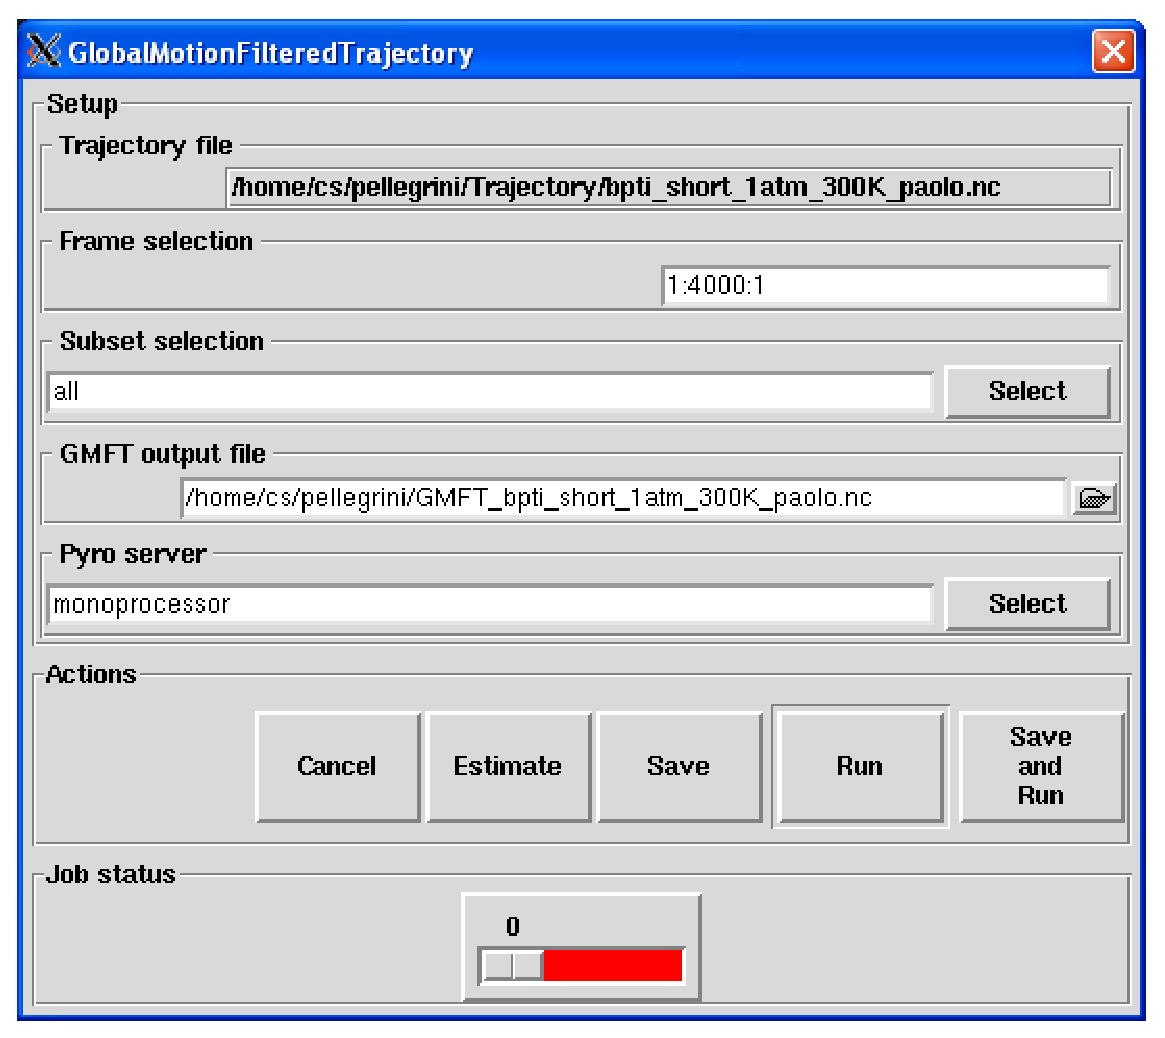
\includegraphics[width=10cm]{Figures/gmft.eps}
\end{center}
\caption[The \textit{GMFT} analysis dialog]{The dialog from where the \textit{GMFT} analysis will be set up and run.}
\label{fig:gmft}
\end{figure}   

The following input fields controls the parameters for the \GMFT\ analysis:

\begin{itemize}
\item \textbf{Trajectory file}\\
\textbf{Format:} string\\
\textbf{Default:} \textit{traj\_file} where \textit{traj\_file} is the name of the loaded trajectory\\
\textbf{Description:} the value of this widget can not be changed. It just recalls for information purpose the name
of the trajectory file loaded for the analysis.

\item \textbf{Frame selection}\\
\textbf{Format:} string\\
\textbf{Default:} \textit{1:traj\_length:1} where \textit{traj\_length} is the number of frames of the trajectory.\\
\textbf{Description:} this widget allows to select the trajectory frames that will be used for the analysis. This must
be a string of the form:
\\\\
\textit{first:last:step}
\\\\
where \textit{first} is an integer specifying the first frame number to consider, \textit{last} is an integer specifying the last 
frame number to consider and \textit{step} is an integer specifying the step number between two frames.

For example,
\begin{itemize}
\item \textit{2:10:3} will select the frames 2, 5 and 8.
\item \textit{1:5:1} will select the frames 1, 2, 3, 4 and 5.
\end{itemize}

\item \textbf{Subset selection}\\
\textbf{Format:} subset selection string\\
\textbf{Default:} \textit{all}\\
\textbf{Description:} this widget allows the selection of a subset of the system for the analysis. 
See Section \ref{subset_selection} for more details.

\item \textbf{GMFT Output file}\\
\textbf{Format:} string\\
\textbf{Default:} \textit{GMFT\_traj\_file.nc} where \textit{traj\_file.nc} is the name of the input trajectory\\
\textbf{Description:} this widget allows to enter the name of the \NetCDF\ output file of the \GMFT\ analysis.
\end{itemize}

\paragraph{Output\\}
The results of a \GMFT\ analysis is a \MMTK\ \NetCDF\ trajectory file containing the trajectory with the global motion filtered 
out.

\subsubsection{Rigid-Body Trajectory}
\label{rbt}
\paragraph{Theory and implementation\\}
\label{rbt_theory}
To analyze the dynamics of complex molecular systems it is often desirable to consider the overall motion of 
molecules or molecular subunits. We will call this motion rigid-body motion in the following. Rigid-body motions 
are fully determined by the dynamics of the centroid, which may be the center-of-mass, and the dynamics of the
angular coordinates describing the orientation of the rigid body. The angular coordinates are the appropriate 
variables to compute angular correlation functions of molecular systems in space and time. In most cases, however, 
these variables are not directly available from \MD\ simulations since \MD\ algorithms typically work in cartesian coordinates. 
Molecules are either treated as flexible, or, if they are treated as rigid, constraints are taken into account in the 
framework of cartesian coordinates \cite{Berendsen}. In \NMOLDYN, \RBT\ can be defined from a 
\MD\ trajectory by fitting rigid reference structures, defining a (sub)molecule, to the corresponding structure in each time 
frame of the trajectory. Here `fit' means the optimal superposition of the structures in a least-squares sense. We will 
describe now how rigid body motions, i.e. global translations and rotations of molecules or  subunits of complex molecules, 
can be extracted from a \MD\ trajectory. A more detailed presentation is given in \cite{Kneller:1991}. We define 
an optimal rigid-body trajectory in the following way: for each time frame of the trajectory the atomic positions of a rigid 
reference structure, defined by the three cartesian components of its centroid (e.g. the center of mass) and three angles, are as 
close as possible to the atomic positions of the corresponding structure in  the \MD\ configuration. Here `as close as possible' means as close 
as possible in a least-squares sense.  

\subparagraph{Optimal superposition.} We consider a given time frame in which the atomic positions of a (sub)molecule are 
given by  ${\bf x}_\alpha,\,\alpha = 1\ldots N$. The corresponding positions in the reference structure are denoted as 
${\bf x}^{(0)}_\alpha,\,\alpha = 1\ldots N$. For both the given structure and the reference structure we introduce the yet 
undetermined centroids ${\bf X}$ and  ${\bf X}^{(0)}$, respectively, and define the deviation 
\begin{equation}
\label{eq:delta}
{\bf \Delta}_\alpha \doteq
{\bf D}({\bf q})\left[{\bf x}^{(0)}_\alpha - {\bf X}^{(0)}\right] -   
       \left[{\bf x}_\alpha - {\bf X}\right].   
\end{equation} 
Here ${\bf D}({\bf q})$ is a rotation matrix which depends on also yet undetermined angular coordinates which we chose to 
be {\em quaternion parameters}, abbreviated as vector ${\bf q} = (q_0,q_1,q_2,q_3)$. The quaternion parameters fulfill the 
normalization condition ${\bf q}\cdot{\bf q} = 1$ \cite{Altmann}. The target function to be minimized is now defined as
\begin{equation}
m({\bf q};{\bf X},{\bf X}^{(0)}) = 
\sum_\alpha \omega_\alpha |{\bf\Delta}|^2_\alpha.
\end{equation}
where $\omega_\alpha$ are atomic weights (see Section \ref{weighting_scheme}). The minimization with respect to the centroids 
is decoupled from the minimization with respect to the quaternion parameters and yields
\begin{eqnarray}
{\bf X}       &= &\sum_\alpha \omega_\alpha\,{\bf x}_\alpha,\\
{\bf X}^{(0)} &= &\sum_\alpha \omega_\alpha\,{\bf x}^{(0)}_\alpha.
\end{eqnarray} 
We are now left with a minimization problem for the rotational part which can be written as
\begin{equation}
\label{eq:minimize_rot}
m({\bf q}) = \sum_\alpha \omega_\alpha 
\left[{\bf D}({\bf q}){\bf r}^{(0)}_\alpha - {\bf r}_\alpha\right]^2
\stackrel{!}{=} Min.
\end{equation}
The relative position vectors
\begin{eqnarray}
{\bf r}_\alpha        &= &{\bf x}_\alpha - {\bf X},\\
{\bf r}^{(0)}_\alpha  &= &{\bf x}^{(0)}_\alpha - {\bf X}^{(0)},
\end{eqnarray} 
are fixed and the rotation matrix reads \cite{Altmann}
\begin{equation}
\label{eq:d_quat}
{\bf D}({\bf q}) = 
\left(
\begin{array}{ccc}
 q_0^2+q_1^2-q^2_2-q^2_3  &2(-q_0q_3+q_1q_2) &2(q_0q_2+q_1q_3) \\
 2(q_0q_3+q_1q_2)  &q_0^2+q_2^2-q^2_1-q^2_3  &2(-q_0q_1+q_2q_3)\\
 2(-q_0q_2+q_1q_3) &2(q_0q_1+q_2q_3)  &q_0^2+q_3^2-q^2_1-q^2_2  
\end{array}
\right).
\end{equation}

\subparagraph{Quaternions and rotations.} The rotational minimization problem can be elegantly solved by using quaternion algebra.
Quaternions are so-called hypercomplex numbers, having a real unit, ${\bf 1}$, and three imaginary units, 
${\bf I}$, ${\bf J}$, and ${\bf K}$. Since ${\bf I}{\bf J} = {\bf K}$ (cyclic), quaternion multiplication is not commutative. 
A possible matrix representation of an arbitrary quaternion,
\begin{equation}
{\bf A} = a_0\cdot{\bf 1} + a_1\cdot{\bf I} + a_2\cdot{\bf J} + 
          a_3\cdot{\bf K},
\end{equation}
reads 
\begin{equation}
\label{eq:a_mat}
 {\bf A} = \left( \begin{array}{rrrr}
                  a_0 &-a_1 &-a_2 &-a_3 \\
                  a_1 & a_0 &-a_3 & a_2 \\
                  a_2 & a_3 & a_0 &-a_1 \\
                  a_3 &-a_2 & a_1 & a_0
                  \end{array} 
           \right).
\end{equation}
The components $a_\nu$ are real numbers. Similarly as normal complex numbers allow one to represent rotations in a plane, quaternions 
allow one to represent rotations in space. Consider the quaternion representation of a vector ${\bf r}$, which is given by 
\begin{equation}
{\bf R} = x\cdot{\bf I} + y\cdot{\bf J} + z\cdot{\bf K},
\end{equation}  
and perform the operation
\begin{equation}
{\bf R}' = {\bf Q}{\bf R}{\bf Q}^T,
\end{equation}  
where ${\bf Q}$ is a normalized quaternion,
\begin{equation}
\|{\bf Q}\|^2 \doteq
q_0^2 + q_1^2 + q_2^2 + q_3^2 = \frac{1}{4}tr\{{\bf Q}^T{\bf Q}\} = 1. 
\end{equation}
The symbol $tr$ stands for `trace'. We note that a normalized quaternion is represented by an {\em orthogonal} $4\times 4$ 
matrix. ${\bf R}'$ may then be written  as
\begin{equation}
{\bf R}' = x'\cdot{\bf I} + y'\cdot{\bf J} + z'\cdot{\bf K},
\end{equation}
where the components $x',y',z'$, abbreviated as ${\bf r}'$, are given by
\begin{equation}
{\bf r}' = {\bf D}({\bf q}){\bf r}.
\end{equation}
The matrix ${\bf D}({\bf q})$ is the rotation matrix defined in
(\ref{eq:d_quat}).

\subparagraph{Solution of the minimization problem.} In quaternion algebra, the rotational minimization problem may now be 
phrased as follows:
\begin{equation}
\label{eq:minimize_rot_quat_1}
m({\bf q}) = \sum_\alpha \omega_\alpha 
\|{\bf Q}{\bf R}^{(0)}_\alpha{\bf Q}^T - {\bf R}_\alpha\|^2
\stackrel{!}{=} Min.
\end{equation}
Since the matrix ${\bf Q}$ representing a normalized quaternion is orthogonal this may also be written as
\begin{equation}
\label{eq:minimize_rot_quat_2}
m({\bf q}) = \sum_\alpha \omega_\alpha 
\|{\bf Q}{\bf R}^{(0)}_\alpha - {\bf R}_\alpha{\bf Q}\|^2.
\stackrel{!}{=} Min.
\end{equation}
This follows from the simple fact that  $\|{\bf A}\| = \|{\bf A}{\bf Q}\|$, if ${\bf Q}$ is normalized. 
Eq. (\ref{eq:minimize_rot_quat_2}) shows that the target function to be minimized can be written as a simple quadratic 
form in the quaternion parameters \cite{Kneller:1991}, \begin{eqnarray}
\label{eq:quad_form}
m({\bf q}) &= &{\bf q}\cdot{\bf M}{\bf q},\\
{\bf M} &= &\sum_\alpha \omega_\alpha {\bf M}_\alpha.
\end{eqnarray}
The matrices ${\bf M}_\alpha$ are positive semi-definite matrices depending on the positions ${\bf r}_\alpha$ and 
${\bf r}^{(0)}_\alpha$:
\begin{equation}
\left.
\begin{array}{lll}
M_{\alpha,11} &= &
  x_\alpha^2 + y_\alpha^2 + z_\alpha^2 
+ x_{0\alpha}^2 + y_{0\alpha}^2 + z_{0\alpha}^2   
-2x_\alpha x_{0\alpha} -2y_\alpha y_{0\alpha} -2z_\alpha z_{0\alpha}
\\
M_{\alpha,12} &= &2(y_\alpha z_{0\alpha} - z_\alpha y_{0\alpha})\\
M_{\alpha,13} &= &2(-x_\alpha z_{0\alpha} + z_\alpha x_{0\alpha})\\
M_{\alpha,14} &= &2(x_\alpha y_{0\alpha} - y_\alpha x_{0\alpha})\\
M_{\alpha,22} &= &
  x_\alpha^2 + y_\alpha^2 + z_\alpha^2 
+ x_{0\alpha}^2 + y_{0\alpha}^2 + z_{0\alpha}^2   
-2x_\alpha x_{0\alpha} +2y_\alpha y_{0\alpha} +2z_\alpha z_{0\alpha}
\\
M_{\alpha,23} &= &-2(x_\alpha y_{0\alpha} + y_\alpha x_{0\alpha})\\
M_{\alpha,24} &= &-2(x_\alpha z_{0\alpha} + z_\alpha x_{0\alpha})\\
M_{\alpha,33} &= &
  x_\alpha^2 + y_\alpha^2 + z_\alpha^2 
+ x_{0\alpha}^2 + y_{0\alpha}^2 + z_{0\alpha}^2   
+2x_\alpha x_{0\alpha} -2y_\alpha y_{0\alpha} +2z_\alpha z_{0\alpha}
\\
M_{\alpha,44} &= &-2(y_\alpha z_{0\alpha} + z_\alpha y_{0\alpha})\\
M_{\alpha,44} &= &
  x_\alpha^2 + y_\alpha^2 + z_\alpha^2 
+ x_{0\alpha}^2 + y_{0\alpha}^2 + z_{0\alpha}^2   
+2x_\alpha x_{0\alpha} +2y_\alpha y_{0\alpha} -2z_\alpha z_{0\alpha}
\\
\end{array}
\right\}
\end{equation}

The rotational fit is now reduced to the problem of finding the minimum of a quadratic form with the constraint that the 
quaternion to be determined must be normalized. Using the method of Lagrange multipliers to account for the normalization 
constraint we have 
\begin{equation}
m'({\bf q},\lambda) = {\bf q}\cdot{\bf M}{\bf q}
- \lambda({\bf q}\cdot{\bf q} - 1) \stackrel{!}{=} Min.
\end{equation}
This leads immediately to the eigenvalue problem
\begin{eqnarray}
{\bf M}{\bf q} &= &\lambda{\bf q},\\
{\bf q}\cdot{\bf q} &= &1.
\end{eqnarray}
Now any normalized eigenvector ${\bf q}$ fulfills the relation $\lambda = {\bf q}\cdot{\bf M}{\bf q} \equiv m({\bf q})$. 
Therefore the eigenvector belonging to the smallest eigenvalue, $\lambda_{min}$, is the desired solution. At the same 
time $\lambda_{min}$ gives the average error per atom.

The result of \RBT\ analysis is stored in a new trajectory file that contains only \RBT\ motions.

\paragraph{Parameters\\}
\label{rbt_parameters}
Pressing the \textbf{Rigid-Body Trajectory} button will pop up the dialog shown on figure \ref{fig:rbt}
\begin{figure}[h!]
\begin{center}
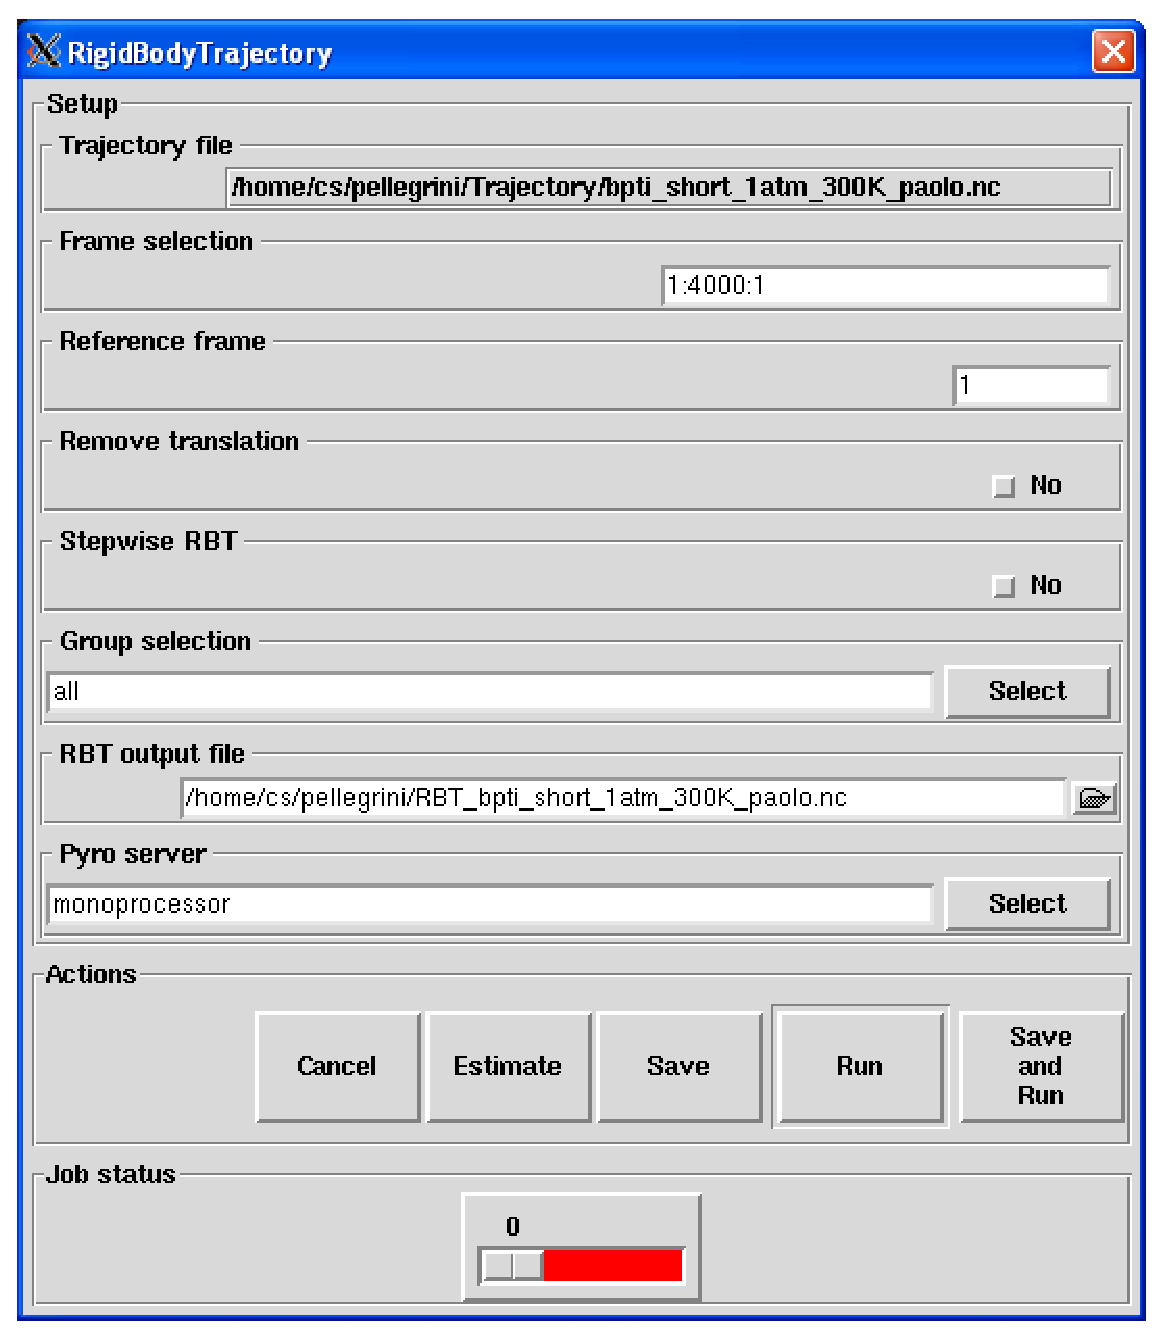
\includegraphics[width=10cm]{Figures/rbt.eps}
\end{center}
\caption[The \textit{RBT} analysis dialog]{The dialog from where the \textit{RBT} analysis will be set up and run.}
\label{fig:rbt}
\end{figure}   

The following input fields controls the parameters for the \RBT\ analysis:

\begin{itemize}
\item \textbf{Trajectory file}\\
\textbf{Format:} string\\
\textbf{Default:} \textit{traj\_file} where \textit{traj\_file} is the name of the loaded trajectory\\
\textbf{Description:} the value of this widget can not be changed. It just recalls for information purpose the name
of the trajectory file loaded for the analysis.

\item \textbf{Frame selection}\\
\textbf{Format:} string\\
\textbf{Default:} \textit{1:traj\_length:1} where \textit{traj\_length} is the number of frames of the trajectory.\\
\textbf{Description:} this widget allows to select the trajectory frames that will be used for the analysis. This must
be a string of the form:
\\\\
\textit{first:last:step}
\\\\
where \textit{first} is an integer specifying the first frame number to consider, \textit{last} is an integer specifying the last 
frame number to consider and \textit{step} is an integer specifying the step number between two frames.

For example,
\begin{itemize}
\item \textit{2:10:3} will select the frames 2, 5 and 8.
\item \textit{1:5:1} will select the frames 1, 2, 3, 4 and 5.
\end{itemize}

\item \textbf{Reference frame}\\
\textbf{Format:} integer in [1,\textit{traj\_length}] where \textit{traj\_length} is the number of frames of the input trajectory\\
\textbf{Default:} \textit{1}\\
\textbf{Description:} this widget allows to specify which frame should be the reference for the \RBT\ analysis.
The value entered should be an integer ranging from 1 to \textit{traj\_length} where \textit{traj\_length} is the 
number of rames of the input trajectory.

\item \textbf{Remove translation}\\
\textbf{Format:} string equal to \textit{yes} or \textit{no}\\
\textbf{Default:} \textit{no}\\
\textbf{Description:} if set to \textit{yes} the translation motion will be removed from the \RBT .

\item \textbf{Stepwise RBT}\\
\textbf{Format:} string equal to \textit{yes} or \textit{no}\\
\textbf{Default:} \textit{no}\\
\textbf{Description:} if set to \textit{yes}, each frame \textit{f} will serve as the reference for the frame \textit{f+1} 
when defining the \RBT\ canceling the value entred in \textbf{Reference frame} entry.

\item \textbf{Group selection}\\
\textbf{Format:} group selection string\\
\textbf{Default:} \textit{all}\\
\textbf{Description:} this widget allows the selection of the groups of atoms that will be defined as rigid-bodies when performing 
the \RBT . See Section \ref{group_selection} for more details.

\item \textbf{RBT output file}\\
\textbf{Format:} string\\
\textbf{Default:} \textit{RBT\_traj\_file.nc} where \textit{traj\_file.nc} is the name of the input trajectory\\
\textbf{Description:} this widget allows to enter the name of the \NetCDF\ output file of the \RBT\ analysis.
\end{itemize}

\paragraph{Output\\}
The results of a \RBT\ analysis is a \MMTK\ \NetCDF\ trajectory file containing the rigid-body trajectory. Beside the 
trajectory, other \NetCDF\ variables are stored in this file namely:
\begin{itemize}
\item groupi, i = 1, 2, \ldots $N_{groups}$: the \MMTK\ indexes of each atom of groups 1, 2, \ldots $N_{groups}$ where 
$N_{groups}$ is the number of groups selected for the analysis,
\item quaternion: a matrix of dimension ($N_{Frames}$, $N_{groups}$, 4) where $N_{Frames}$ is the number of selected frames for the \RBT\ 
analysis. This matrix contains the quaternions produced by the \RBT\ analysis at each frame and for each rigid-body,
\item cms: a matrix of dimension ($N_{Frames}$, $N_{groups}$, 3) that contains the coordinates of the center of mass of each 
rigid-body for each frame,
\item fit: a matrix of dimension ($N_{Frames}$, $N_{groups}$) that contains the results of the fit produced by the \RBT\ 
fitting procedure at each frame and for each rigid-body.
\end{itemize}

\subsubsection{Center Of Mass Trajectory}
\label{comt}
\paragraph{Theory and implementation\\}
\label{comt_theory}
The \COMT\ analysis consists in deriving the trajectory of the respective centers of mass of a 
set of groups of atoms. In order to produce a visualizable trajectory, \NMOLDYN\ assigns the centers of mass to 
pseudo-hydrogen atoms whose mass is equal to the mass of their associated group. Thus, the produced trajectory can be reused 
for other analysis. In that sense, \COMT\ analysis is a practical way to reduce noticeably the dimensionality of a system.

\paragraph{Parameters\\}
\label{comt_parameters}
Pressing the \textbf{Center Of Mass Trajectory} button will pop up the dialog shown on figure \ref{fig:comt}
\begin{figure}[h!]
\begin{center}
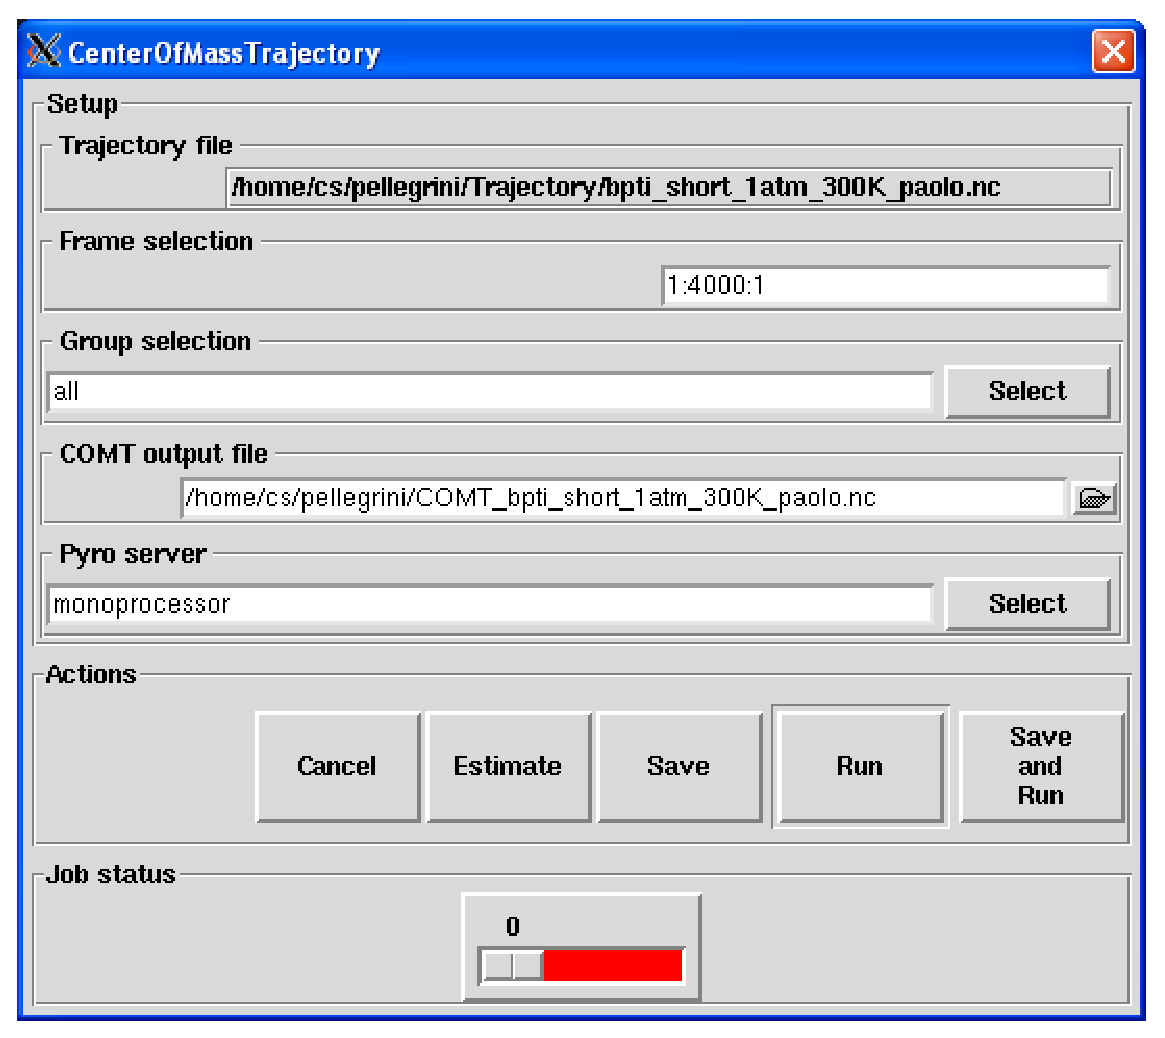
\includegraphics[width=10cm]{Figures/comt.eps}
\end{center}
\caption[The \textit{COMT} analysis dialog]{The dialog from where the \textit{COMT} analysis will be set up and run.}
\label{fig:comt}
\end{figure}

The following input fields controls the parameters for the \COMT\ analysis:

\begin{itemize}
\item \textbf{Trajectory file}\\
\textbf{Format:} string\\
\textbf{Default:} \textit{traj\_file} where \textit{traj\_file} is the name of the loaded trajectory\\
\textbf{Description:} the value of this widget can not be changed. It just recalls for information purpose the name
of the trajectory file loaded for the analysis.

\item \textbf{Frame selection}\\
\textbf{Format:} string\\
\textbf{Default:} \textit{1:traj\_length:1} where \textit{traj\_length} is the number of frames of the trajectory.\\
\textbf{Description:} this widget allows to select the trajectory frames that will be used for the analysis. This must
be a string of the form:
\\\\
\textit{first:last:step}
\\\\
where \textit{first} is an integer specifying the first frame number to consider, \textit{last} is an integer specifying the last 
frame number to consider and \textit{step} is an integer specifying the step number between two frames.

For example,
\begin{itemize}
\item \textit{2:10:3} will select the frames 2, 5 and 8.
\item \textit{1:5:1} will select the frames 1, 2, 3, 4 and 5.
\end{itemize}

\item \textbf{Group selection}\\
\textbf{Format:} group selection string\\
\textbf{Default:} \textit{all}\\
\textbf{Description:} this widget allows the selection of the groups of atoms whose trajectories of their centers of mass 
will define the \COMT . See Section \ref{group_selection} for more details.

\item \textbf{COMT output file}\\
\textbf{Format:} string\\
\textbf{Default:} \textit{COMT\_traj\_file.nc} where \textit{traj\_file.nc} is the name of the input trajectory\\
\textbf{Description:} this widget allows to enter the name of the \NetCDF\ output file of the \COMT\ analysis.
\end{itemize}

\paragraph{Output\\}
The results of a \COMT\ analysis is a \MMTK\ \NetCDF\ trajectory file containing the trajectory of the centers of mass of 
each selected group of atoms.

\subsubsection{Auto-Regressive Analysis}
\label{ara}
\paragraph{Theory and implementation\\}
\label{ara_theory}
The concept of \ARA\ analysis is intimitely related to the one of memory function. Memory functions have 
been used for a long time in theoretical statistical physics to describe the time dependence of autocorrelation
functions. Nevertheless, the use of memory functions in the context of \MD\ simulations has been hindered by the lack of a 
suitable numerical algorithm for their calculation. Such an algorithm has been published and is now implemented in 
\NMOLDYN\ \cite{Hinsen:2001}. The key point is that a reliable estimates for memory functions can be obtained by assuming 
an \AR\ model for the underlying stochastic process and not for the memory function itself.

To compute the memory function $\xi(t)$ from a discrete time serie $x(n) \equiv x(n\Delta t)$ the latter is modelled by an 
{\em autoregressive stochastic process} of order \textit{P} \cite{Papoulis:1991,Makhoul:1975},
\begin{equation}
\label{eq:ar}
x(t) = \sum_{n=1}^P a^{(P)}_n x(t- n \Delta t) + \epsilon_P(t).
\end{equation}
Here $\epsilon_P(t)$ is {\em white noise} with zero mean and amplitude
$\sigma_P$. The coeffients $\{a^{(P)}_n\}$ are fitted to the discrete time serie using Burg's algorithm \cite{Burg,Makhoul:1977}, 
and $\sigma_P$ is given by
\begin{equation}
\sigma_P^2=r(0)-\sum_{n=1}^P a_n^{(P)} \mathrm(n\Delta t),
\end{equation}
where $r(t)$ is the autocorrelation function of $x(t)$
\begin{equation}
r(t) :=\langle x(t)x(0)\rangle. 
\end{equation}
In all following calculations \NMOLDYN\ works with a set of coefficients $\{a_n\}$ which has been averaged over all 
selected atoms and the three Cartesian coordinates.

\subparagraph{VACF within the AR model} The autocorrelation function $r(t)$ introduced in the previous Section is here 
the \emph{normalized} \VACF 
\begin{equation}
VACF(t) := \frac{\langle v(t)v(0)\rangle}{\langle v^2(0)\rangle}
\end{equation}
hence $r(0)=VACF(0)=1$. 
Here $v(t)$ is the x-, y-, or z-component of the velocity of a `tagged' atom. 
The memory function $\xi(t)$ of $\psi(t)$ is defined by the relation
\begin{equation}
\label{eq:memory_function_equation}
\frac{d}{dt}\VACF(t) = -\int_{0}^{t}d\tau\, \xi(t-\tau)\VACF(\tau).
\end{equation}
Eq. (\ref{eq:memory_function_equation}) is called the {\em memory function equation}. 

Within the AR-model the z-transform of the \VACF\ has the form
\begin{equation}
\label{eq:vacf_ar}
\mathrm{VACF}^{(AR)}(z) = \frac{1}{a^{(P)}_P}\frac{-z^P\sigma_P^2}
{\prod_{k=1}^P (z-z_k)\,\prod_{l=1}^P(z-z^{-1}_l)}.
\end{equation}
Here the $\{z_k\}$ are the zeros of
\begin{equation}
\label{eq:p_z}
p(z) = z^P-\sum_{k=1}^{P}a^{(P)}_k z^{P-k}.
\end{equation}
We recall that the z-transform of an arbitrary discrete function $f(n)$ is given by 
$F(z) = \sum_{n=-\infty}^{+\infty} f(n) z^{-n}$, and the inverse transform by $f(n)  = \frac{1}{2\pi i}\oint_C dz\,z^{n-1} 
F(z)$. Applying the inverse z-transform to (\ref{eq:vacf_ar}) yields
\begin{equation}
\label{eq:psi_n}
VACF^{(AR)}(n) = \sum_{j=1}^{P}\beta_jz_j^{|n|},
\end{equation}
where the coefficients $\beta_j$ are given by
\begin{equation}
\label{eq:beta_j}
\beta_j = \frac{1}{a_P}\frac{-z_j^{P-1}\sigma_P^2}
{\prod_{k=1,k\ne j}^P (z_j-z_k)\,\prod_{l=1}^P(z_j-z^{-1}_l)}.
\end{equation}
Note that $VACF^{(AR)}(n)$ has a multiexponential form, and that the stability criterion
\begin{equation}
\label{eq:stability}
|z_j| < 1,\quad j=1,\ldots,P,
\end{equation}
must be fulfilled. This is guaranteed by the Burg-algorithm \cite{Burg,Makhoul:1977}. 

\subparagraph{Density of states within the AR model} Evaluating $\mathrm{VACF}^{(AR)}(z)$ as given by (\ref{eq:vacf_ar}) at
$z=\exp(i\omega\Delta t)$ yields the density of states within the AR
model:
\begin{equation}
DOS^{(AR)}(\omega)=\frac{\Delta t}{2}\frac{k_BT}{M} \mathrm{VACF}^{(AR)}
\left(\exp[i\omega\Delta t]\right).
\end{equation}
Here $M$ is the mass of the tagged atom, $k_B$ is the Boltzmann constant, and $T$ the temperature. Note that the \VACF\ and 
the density of states within the \AR\ model are entirely determined by the coefficients $a^{(P)}_n$.

\subparagraph{Discrete memory function of the VACF within the AR model}
Starting from the memory function equation of the \VACF\ (Eq. \ref{eq:memory_function_equation}), the first step towards a 
numerical computation of the memory function consists in discretizing Eq. \ref{eq:memory_function_equation} 
\begin{equation}
\label{eq:memory_function_discrete}
\frac{VACF(n+1)-VACF(n)}{\Delta t} = -\sum_{k=0}^{n-1} 
\Delta t\,\xi(n-k)\psi(k),
\end{equation}
Eq. (\ref{eq:memory_function_discrete}) is now subjected to a {\em one-sided} z-transform. Using that
\begin{equation}
Z_{>}\left\{f(n+1)-f(n)\right\} = 
zF_{>}(z) - zf(0)
\end{equation}
for any discrete function $f(n)$ whose one-sided z-transform exists, one obtains from (\ref{eq:memory_function_discrete})
\begin{equation}
\label{eq:xi_z}
\Xi_{>}(z) = \frac{1}{\Delta t^2} \left(\frac{z}{\mathrm{VACF}_{>}(z)} + 1 -
z\right),
\end{equation}
using that $VACF(0)=1$. The one-sided z-transform of an arbitrary discrete function $f(n)$ is defined as 
$F_{>}(z) = \sum_{n=0}^{\infty} f(n) z^{-n}$.
Here it has been used that the one-sided z-transform of the discrete convolution integral is just the product 
$\Xi_{>}(z)\mathrm{VACF}_{>}(z)$. Inserting the definition of the one-sided \textit{z}-transform for $\Xi_{>}(z)$ and 
$\mathrm{VACF}_{>}(z)$, this equation can be rewritten as
\begin{equation}
  \label{eq:m_t}
  \sum_{j=0}^\infty ~ \xi(j) \, z^{-j} = \frac{1}{\Delta t^2} \,
  \frac{\sum_{j=0}^\infty \, \left[VACF(j) - VACF(j+1)\right] \, z^{-j}}
  { \sum_{j=0}^\infty \, VACF(j) \, z^{-j} }. 
\end{equation}
Note that the term proportional to \textit{z} cancels out.  The time dependent memory function is, in principle, obtained by 
comparing the coefficients of the series on the {\em lhs} and the {\em rhs} of Eq. (\ref{eq:m_t}). To construct a numerical method, 
we replace the series by polynomials of order \textit{N}, where $t=N\Delta t$ defines the time window for the memory function to be computed. 
After this first step a polynomial division is performed on the {\em rhs} of Eq. (\ref{eq:m_t}), and after a subsequent multiplication 
of both sides with $z^{-N}$ one obtains the time dependent memory function, $\xi(j)$, by comparison of coefficients,
\begin{eqnarray}
\label{eq:xi_division}
  \frac{z^{-N}}{\Delta t^2}\,\frac{\sum_{j=0}^N \, \left[VACF(j) -
    VACF(j+1)\right] \, z^{N-j}} { \sum_{j=0}^N \, VACF(j) \,
    z^{-j}} &=&
  z^{-N} \left(\sum_{j=0}^N \, c_j \, z^{N-j} + R \right)\nonumber\\
  &=& \sum_{j=0}^N \xi(j) \, z^{-j}.
\end{eqnarray}

Within \NMOLDYN\ $VACF(n)$ is replaced by the autocorrelation function calculated in the framework of the autoregressive model, 
$VACF^{(AR)}(n)$, as in Eqs. \ref{eq:psi_n} and \ref{eq:beta_j}. The coefficients $c_j$ are obtained by polynomial division and 
$R$ is a rest which does not contain information on the memory function within the time interval $t\in [0,N\Delta t]$. The discrete 
memory function is therefore given by $\xi(j) = c_{N-j}$.

A remark concerning the discretization scheme (\ref{eq:memory_function_discrete}) is in place here. The discrete convolution 
sum is effectively a first order approximation of the convolution integral. More sophisticated approximations could be used,
but they would lead to less convenient expressions upon z-transformation. Correspondingly, we have chosen a first order 
approximation for the differentiation on the left-hand side of (\ref{eq:memory_function_equation}). In this way the first order 
(integro-)differential equation (\ref{eq:memory_function_equation}) is transformed into the first order difference equation 
(\ref{eq:memory_function_discrete}).

However, this simple discretization scheme together with the use of the one-sided \textit{z}-transform leads to a significant 
error in $\xi(0)$. It is clear from Eq. (\ref{eq:memory_function_equation}) that due to the symmetry of the autocorrelation function 
($\psi(t)=\psi(-t)$), the derivative $d\psi/dt$ should vanish at $t=0.$ However, in the discretized version it is 
approximated by a forward difference that is always negative. A higher-order calculation shows that the estimate for 
$\xi(0)$ that results from the procedure described above should be doubled.

\subparagraph{MSD within the AR model} The relation between the \VACF\ and the \MSD\ reads
\begin{equation}
\label{eq:msd_vacf_x}
{MSD}(t)=\langle[x(t)-x(0)]^2\rangle=2 \int_{0}^{t}d\tau\,(t - \tau)
C_{vv}(t)
\end{equation}
By discretizing the above equation one obtains
\begin{equation}
\label{eq:msd_vacf_x_discrete_1}
MSD(n)=2 \sum_{k=0}^n \Delta t^2(n-k)C_{vv}(k).
\end{equation}
Using
\begin{eqnarray}
f_1(n)=\Theta(n)\cdot n
f_2(n)=\Theta(n)\cdot C_{vv}(n)
\end{eqnarray}
into Eq. \ref{eq:msd_vacf_x_discrete_1}, gives
\begin{equation}
\label{eq:msd_vacf_x_discrete_2}
MSD(n)=2 \sum_{k=-\infty}^{+\infty} \Delta t^2f_1(n-k)f_2(k)
\end{equation}
Making use of the one-side z-transform (equivalent to the Laplace transform for discrete functions), we obtain 
\begin{equation}
\label{eq:msd_vacf_x_discrete_2_Z}
{MSD}^{>}(z)= 2 F_1^{>} F_2^{>}\Delta t^2 ,
\end{equation}
where
\begin{equation}
\label{eq:f1z}
F_1^{>}=\frac{z}{(z-1)^2}.
\end{equation}
Introducing Eq. \ref{eq:f1z} into Eq. \ref{eq:msd_vacf_x_discrete_2_Z} yields
\begin{equation}
\label{msd_z}
MSD^{>}(z)= 2 \frac{z\Delta t^2}{(z-1)^2}C_{vv}^{>}(z)
\end{equation}
and its inverse z-transform reads
\begin{equation}
\label{inv_Z}
{MSD}(n)= 2\Delta t^2\cdot\frac{1}{2\pi i}\oint dz z^{n-1}\cdot\frac{z}{(z-1)^2}\cdot C_{vv}^{>}(z).
\end{equation}
Using the expression of the non-normalized $C_{vv}^{\rangle}(z)$ obtained in the framework of the \AR\ model 
\begin{equation}
C_{vv}^{>}(z)= \sum_{j=1}^P\beta_j\frac{z}{z-z_j}\cdot\langle v^2\rangle
\end{equation}
one finds the expression of \MSD\ within the same \AR\ model
\begin{eqnarray}
MSD^{AR}(n) & = & 2\Delta t^2\langle v^2\rangle \sum_{j=1}^P\beta_j \frac{1}{2\pi i}\oint dz \frac{z^{n+1}}{(z-1)^2}\cdot\frac{1}{z-z_j}\\
& = & 2\Delta t^2\langle v^2\rangle \sum_{j=1}^P\beta_j \{\frac{n}{1-z_j}-\frac{z_j}{(1-z_j)^2}+\frac{z_j^{n+1}}{(1-z_j)^2}\}.
\end{eqnarray}
\begin{equation}
MSD^{AR}(n)\stackrel{n\rightarrow +\infty}{\simeq} 2Dn\Delta t \mbox{  ;  } 
D=\Delta t\langle v^2\rangle \sum_{j=1}^P\frac{\beta_j}{1-z_j}=\frac{\langle v^2\rangle}{\gamma}
\end{equation}
which allows one to compute the \MSD\ within the \AR\ model from the poles and the $\beta_j$ coefficients of the non-normalized \VACF.

\subparagraph{Friction coefficient within the AR model} The friction coefficient is defined as the integral over 
the memory function. In the discrete case we write
\begin{equation}
\label{eq:xi_0}
\xi_0 := \sum_{n=0}^{\infty}\Delta t\:\xi(n) = 
\Delta t\,\Xi_{>}(1).
\end{equation}
As shown in \cite{Hinsen:2001}, the \AR\ model allows us to express ${\Psi_{>}(z)}$ as
\begin{equation}
\label{eq:psi_ar_z}
\mathrm{VACF}^{(AR)}_{>}(z)=\sum_{n=0}^{\infty}VACF^{(AR)}(n) z^{-n} = \sum_{j=1}^{P}\beta_j \frac{z_j}{z-z_j},
\end{equation} 
where the coefficients $\beta_j$ are given by eq. (\ref{eq:beta_j}), and the roots $z_j$ must fulfill the stability 
criterion (\ref{eq:stability}).
Inserting (\ref{eq:psi_ar_z}) into (\ref{eq:xi_z}) yields $\Xi^{(AR)}_{>}(z)$, the z-transform of the discrete memory 
function within the \AR\ model,
\begin{equation}
\label{eq:xi_ar_z}
\Xi^{(AR)}_{>}(z) = \frac{1}{\Delta t^2}
\left(\frac{z}{\mathrm{VACF}^{(AR)}_{>}(z)} + 1 - z\right).
\end{equation}
Using (\ref{eq:xi_ar_z}) we obtain thus within the \AR\ model
\begin{equation}
\label{eq:xi_0_2}
\xi^{(AR)}_0 = \frac{1}{\Delta t}
\frac{1}{\sum_{j=1}^{P}\beta_j\frac{1}{1-z_j}}.
\end{equation}
This shows that $\xi_0$ can be obtained from the zeros $z_j$ of the characteristic polynomial $p(z)$, defined in (\ref{eq:p_z}).

In the framework of the autoregressive model, \NMOLDYN\ allows one to calculate the \VACF, the \VACF\ memory function, the 
\DOS , the \MSD , and the \AR\ coefficients $a_n^{(P)}$ of the velocity trajectory, averaged over all selected atoms 
and three Cartesian coordinates. 

\paragraph{Parameters\\}
\label{ara_parameters}
Pressing the \textbf{Auto-Regressive Analysis} button will pop up the dialog shown on figure \ref{fig:ara}
\begin{figure}[h!]
\begin{center}
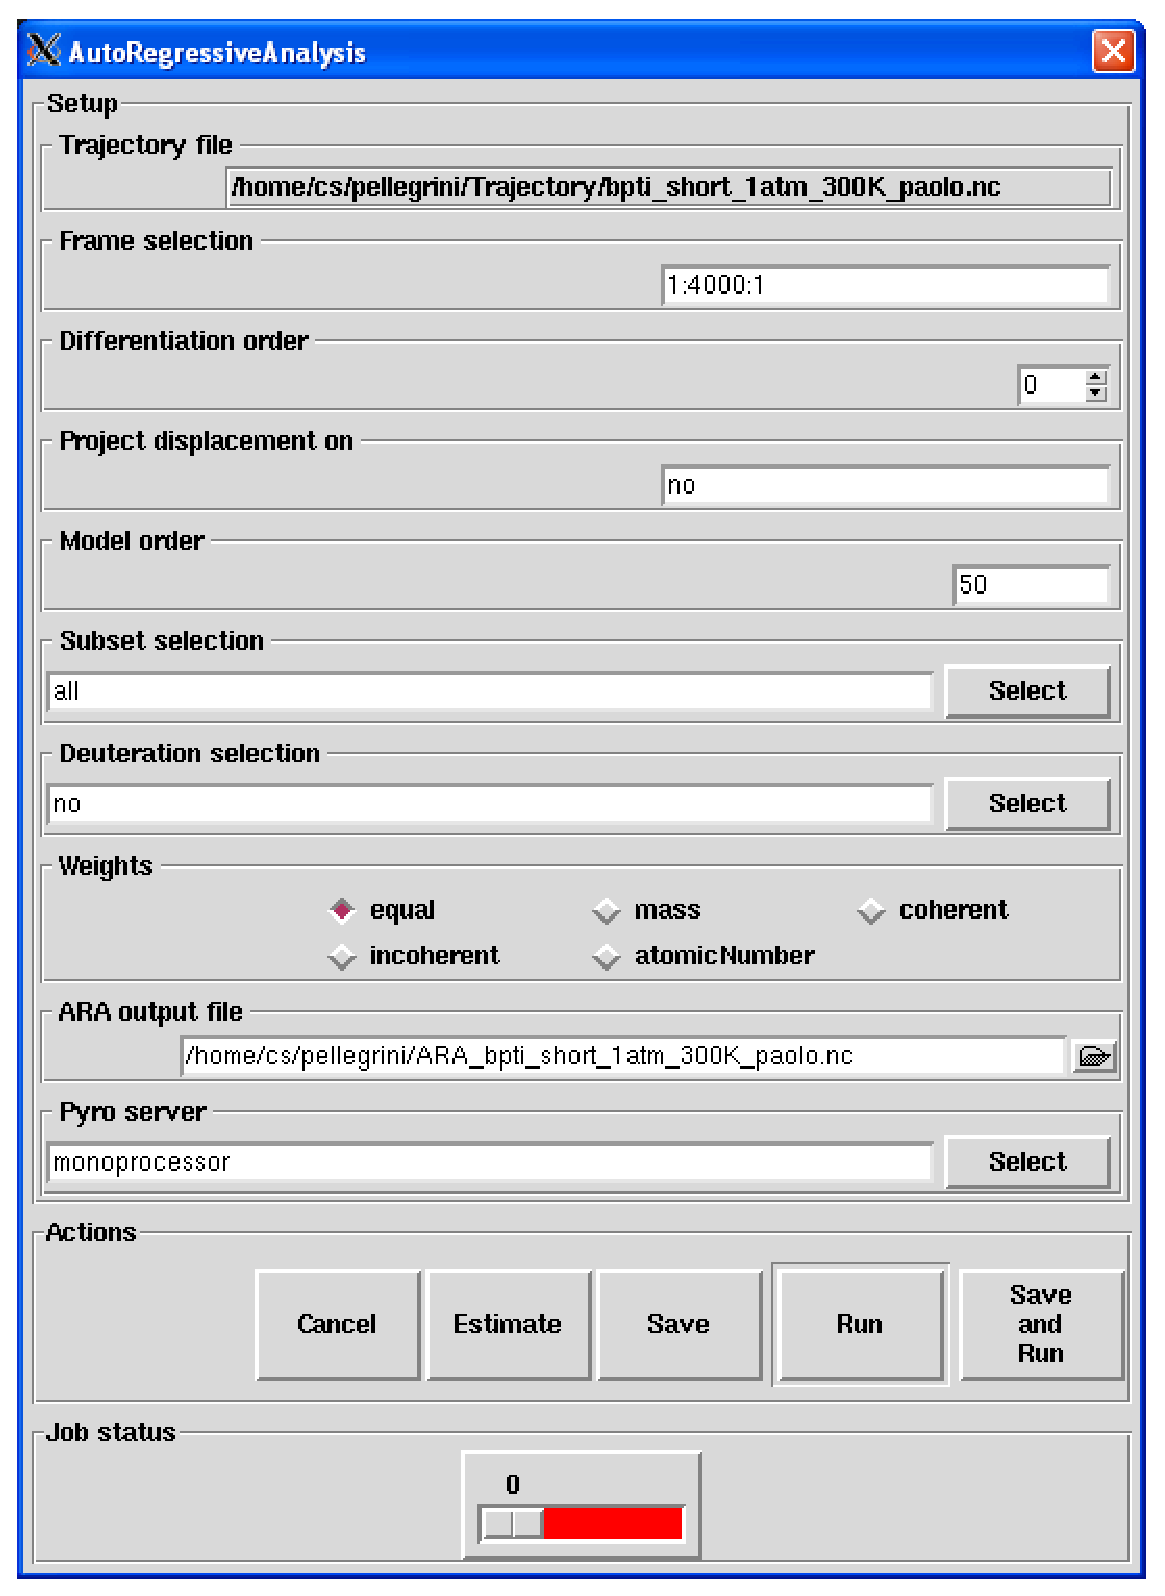
\includegraphics[width=10cm]{Figures/ara.eps}
\end{center}
\caption[The \textit{ARA} analysis dialog]{The dialog from where the \textit{ARA} analysis will be set up and run.}
\label{fig:ara}
\end{figure}

The following input fields controls the parameters for the \ARA\ analysis:

\begin{itemize}
\item \textbf{Trajectory file}\\
\textbf{Format:} string\\
\textbf{Default:} \textit{traj\_file} where \textit{traj\_file} is the name of the loaded trajectory\\
\textbf{Description:} the value of this widget can not be changed. It just recalls for information purpose the name
of the trajectory file loaded for the analysis.

\item \textbf{Frame selection}\\
\textbf{Format:} string\\
\textbf{Default:} \textit{1:traj\_length:1} where \textit{traj\_length} is the number of frames of the trajectory.\\
\textbf{Description:} this widget allows to select the trajectory frames that will be used for the analysis. This must
be a string of the form:
\\\\
\textit{first:last:step}
\\\\
where \textit{first} is an integer specifying the first frame number to consider, \textit{last} is an integer specifying the last 
frame number to consider and \textit{step} is an integer specifying the step number between two frames.

For example,
\begin{itemize}
\item \textit{2:10:3} will select the frames 2, 5 and 8.
\item \textit{1:5:1} will select the frames 1, 2, 3, 4 and 5.
\end{itemize}

\item \textbf{Differentiation order}\\
\textbf{Format:} integer in [0,5]\\
\textbf{Default:} 0 if velocities are stored in the trajectory file, 1 otherwise\\
\textbf{Description:} this widget allows to specify the order of the derivation scheme used to get the velocities out 
of the coordinates. If your trajectory \NetCDF\ file already contains the velocities then just select \textit{0}.
However, you can still decide to get the velocities out of the coordinates. In that case, \NMOLDYN\ performs a numerical 
differentiation of the input data. To do so, \NMOLDYN\ can perform numerical differentiation from order \textit{1} to 
order \textit{5}. Using order \textit{1}, the first time derivative of each point $r(t_i)$ 
is calculated as
\begin{equation}
\dot{r}(t_i)=\frac{r(t_{i+1})-r(t_{i})} {\Delta t},
\end{equation}
where $\Delta t$ is the time step. 
Choosing order \textit{N} with \textit{N=2,...,5}, \NMOLDYN\ calculates the first time-derivative of each point 
$r(t_i)$ ($r=x,y,z$) using the \textit{N}-order polynomial interpolating the \textit{N+1} points across $r(t_i)$, where $r(t_i)$ 
belongs to this set \cite{Abramowitz}.

\item \textbf{Project displacement on}\\
\textbf{Format:} string\\
\textbf{Default:} \textit{no}\\
\textbf{Description:} this widget allows to specify a vector along which the \ARA\ will be computed. This vector does not 
need to be normalized as \NMOLDYN\ will perform the normalization when processing it. The entered value must have the 
following format:
\\\\
\textit{vx:vy:vz}
\\\\
where \textit{vx}, \textit{vy} and \textit{vz} are floats that represent respectively the \textit{x}, \textit{y} and \textit{z} coordinates of the vector.

\item \textbf{Model order}\\
\textbf{Format:} integer in [1,$N_{frames}$[ where $N_{frames}$ is the number of selected frames for the analysis\\
\textbf{Default:} \textit{50}\\
\textbf{Description:} this widget allows to specify \textit{P}, the order (= poles number) of the autoregressive model. {\it A priori} 
the autocorrelation function and its power spectrum can be approximated to almost arbitrary precision by increasing the 
order of the autoregressive model. In practice it has been proven that reliably computation can be carried out up to \textit{P} of 
the order of 1000 poles.

\item \textbf{Subset selection}\\
\textbf{Format:} subset selection string\\
\textbf{Default:} \textit{all}\\
\textbf{Description:} this widget allows the selection of a subset of the system for the analysis. 
See Section \ref{subset_selection} for more details.

\item \textbf{Deuteration selection}\\
\textbf{Format:} deuteration selection string\\
\textbf{Default:} \textit{no}\\
\textbf{Description:} this widget allows the selection of a subset hydrogen atoms that will take the atomic parameters 
of deuterium. See Section \ref{deuteration_selection} for more details.

\item \textbf{Weights}\\
\textbf{Format:} string equal to \textit{equal}, \textit{mass}, \textit{coherent}, \textit{incoherent} or \textit{atomicNumber}\\
\textbf{Default:} \textit{equal}\\
\textbf{Description:} this widget allows the selection of the weighting scheme to apply on each atomic contribution 
to the various properties computed through \ARA\ analysis (\MSD , \VACF , \DOS ,). See Section \ref{weighting_scheme} for more 
details. 

\item \textbf{ARA output file}\\
\textbf{Format:} string\\
\textbf{Default:} \textit{ARA\_traj\_file.nc} where \textit{traj\_file.nc} is the name of the input trajectory\\
\textbf{Description:} this widget allows to enter the name of the \NetCDF\ output file of the \ARA\ analysis. A \CDL\ 
version of the \NetCDF\ output file is also automatically created with \textit{ARA\_traj\_file.cdl} name.
\end{itemize}

\paragraph{Output\\}
The results of an \ARA\ analysis are stored in a \NetCDF\ file whose main variables are namely:
\begin{itemize}
\item time\_vacf: the times in \ps\ at which the autoregressive \VACF\ was evaluated,
\item vacf: the corresponding autoregressive \VACF\ in \vacfunits ,
\item frequency: the frequencies in \thz\ at which the autoregressive \DOS\ was evaluated,
\item dos: the corresponding autoregressive \DOS,
\item time\_msd: the times in \ps\ at which the autoregressive \MSD\ was evaluated,
\item msd: the corresponding autoregressive \MSD\ in \nmsquare ,
\item time\_memory: the times in \ps\ at which the autoregressive \VACF\ memory function was evaluated,
\item memory\_function: the corresponding autoregressive \VACF\ memory function,
\item n: the index for the autoregressive coefficients $a_n^{(P)}$,
\item ar\_coefficients: the autoregressive coefficients $a_n^{(P)}$.
\end{itemize}

\subsubsection{Quasi Harmonic Analysis}
\label{qha}
\paragraph{Theory and implementation\\}
\label{qha_theory}
\QHA\ is a method for obtaining effective modes of vibration from fluctuations calculated by a \MD\ 
simulation. The underlying principle is that from atomic fluctuations, an effective force field can be calculated 
relative to the average dynamic structure that yields the same fluctuation matrix as that obtained from a normal mode 
calculation. Since the fluctuation matrix is inversely proportional to the effective force constant matrix, they have common 
eigenvectors which correspond to the quasiharmonic modes of vibration. Quasiharmonic modes  can be analyzed in the same way 
as normal modes, and comparison of the results with those from harmonic approximation calculations for the same system is 
straightforward.

The way to perform a \QHA\ in \NMOLDYN\ is based on the diagonalization of the fluctuation matrix that can be easily retrieved 
from a \MD\ simulation. Indeed, from a \MD\ simulation, coordinates which define the position of all atoms as a function of time are
saved at each step of the \MD . From these coordinates, both the average position $\langle \mathbf{x} \rangle$ and the 
covariance matrix of fluctuations about the average position $\sigma$  can be calculated the latter being defined as:
\begin{equation}
\sigma_{ij} = \left\langle \left ( x_{i} - \langle x \rangle \right ) \left ( x_{j} - \langle x \rangle \right )\right\rangle
\end{equation}
with variances as the diagonal elements and with covariances as the off-diagonal elements.

Once the covariance matrix of fluctuations is obtained, the Quasi-Harmonic modes of vibration $\Delta x$ and their 
corresponding frequencies $\omega$ are calculated by solving (diagonalizing) the equation:
\begin{equation}
\label{eq:qha}
\left ( \mathbf{\sigma^{\prime}} - \lambda^{\prime} \mathbf{I}\right )\mathbf{\eta} = 0
\end{equation}
where $\mathbf{I}$ is the identity matrix and 
\begin{equation}
\mathbf{\sigma^{\prime}} = \mathbf{M^{1/2}} \mathbf{\sigma} \mathbf{M^{1/2}}
\end{equation}
$\mathbf{M}$ being the diagonal mass matrix.

The solutions of \ref{eq:qha} yielding:
\begin{equation}
\label{eq:qha_omega}
\omega = \left (k_{B}T/\lambda^{\prime} \right )^{1/2}
\end{equation}
and
\begin{equation}
\label{eq:qha_dx}
\mathbf{\Delta x} = \mathbf{M}^{-1/2}\mathbf{\eta}
\end{equation}

Once the normal modes have been obtained, a great variety of analysis can be performed. \NMOLDYN\ proposes some of 
them namely:
\begin{itemize}
\item Local and global character indicator

Normal modes of vibration can involve all the atoms of the system, as in the case of low-frequency global deformation motions, or 
be localized in one particular part of the molecule. It is useful to have indicators which define the degree of global character or local 
character for particular modes of vibration. Since the eigen vectors form an orthonormal basis 
$\sum_{j = 1}^{3N} \Delta x_{ji}^2 = 1$ where \textit{N} is the number of selected atoms, a local character indicator is given by:
\begin{equation}
\label{eq:qha_lci}
lci = \sum_{j = 1}^{3N} \Delta x_{ji}^4
\end{equation}
which is large for modes \textit{i} with significant local character. The global character indicator is given by:
\begin{equation}
\label{eq:qha_gci}
gci = \sum_{j = 1}^{3N} \frac{|\Delta x_{ji}|}{\sqrt{3N}}^{-4}
\end{equation}
which is large for modes \textit{i} without significant global character. These indicators are not invariant with the orientation of the 
system and are only qualitative indicators of character because only the sum of the squares is invariant to rotation. If the motion is 
dominated by a single component of a single-atom, then $\Delta x_i$ will be close to unity for that element and zero for all others. This
results in the maximum possible value for the local characteer indicator of 1 and a maximum for the lack of global character 
indicator of $9N^2$. The other extreme is represented by a net translation of all atoms in the \textit{(1,1,1)} direction, where all elements are the 
same with a value of $\sqrt{3N}$. In this case the local character indicator has a minimum value of $3N^{-1}$ and the lack of global character 
indicator will hav a minimum of 1. Modes with significant mixing of global and local character may have a large local indicator and a small lack of global 
character indicator; thus two indicators are needed to evaluate the character of the motion.

\item Projection of \MD\ trajectories onto normal modes

It is useful to compare normal modes of vibration (or other type of motion) with the \MD\ simulation. This allows examination of the 
amplitudes of this type of motion and the time scales. This is a straightforward procedure in which the effects of solvent damping may be explored for the *
case in which the \MD\ simulation is carried out with explicit solvent even if the normal mode calculation is carried out in vaccuum. The procedure 
is to generate a time series of the projection of the difference of trajectory position and the average position into a mode of interest given by:
\begin{equation}
\label{eq:qha_at}
A_a(t) = \sum_{i=1}^{3N} \Delta x_{ai} M_i^{\frac{1}{2}} \left(x_i(t) - \langle x_i\rangle\right)
\end{equation}
This time series can be evaluated with standard procedures to determine correlation functions and spectra. It is also useful in analyzing the 
results of a \QHA\ analysis to determine which modes are predominantly vibrational in character and which arise mainly from jumping between energy 
substates.
\end{itemize}

Beside the quantitative analysis described above, one of the best way to understand a normal mode of vibration is through a 
visual examination. To do this, a trajectory must be created which depicts the molecular system as a function of time from a 
given starting configuration. For a set of normal modes to view, this trajectory is given by:
\begin{equation}
\label{eq:qha_trajectory}
\textbf{x}(t) = \langle \textbf{x} \rangle + \sum_{i=1}^{N_{modes}} \alpha_i M^{-\frac{1}{2}}\Delta x_i cos(\omega_i t)
\end{equation}
where $\alpha_i$ and $\omega_i$ are respectively the amplitude and frequency of the motion associated to normal mode $i$ and 
$N_{modes}$ is the number of selected normal modes to visualize. \NMOLDYN\ allows the visualization of normal modes through a 
specific viewer (see Section \ref{effective_mode}).

For more details about QHA and related techniques please refer to Ref. \cite{Karplus}

\paragraph{Parameters\\}
\label{qha_parameters}
Pressing the \textbf{Quasi-Harmonic analysis} button will pop up the dialog shown on figure \ref{fig:qha}
\begin{figure}[h!]
\begin{center}
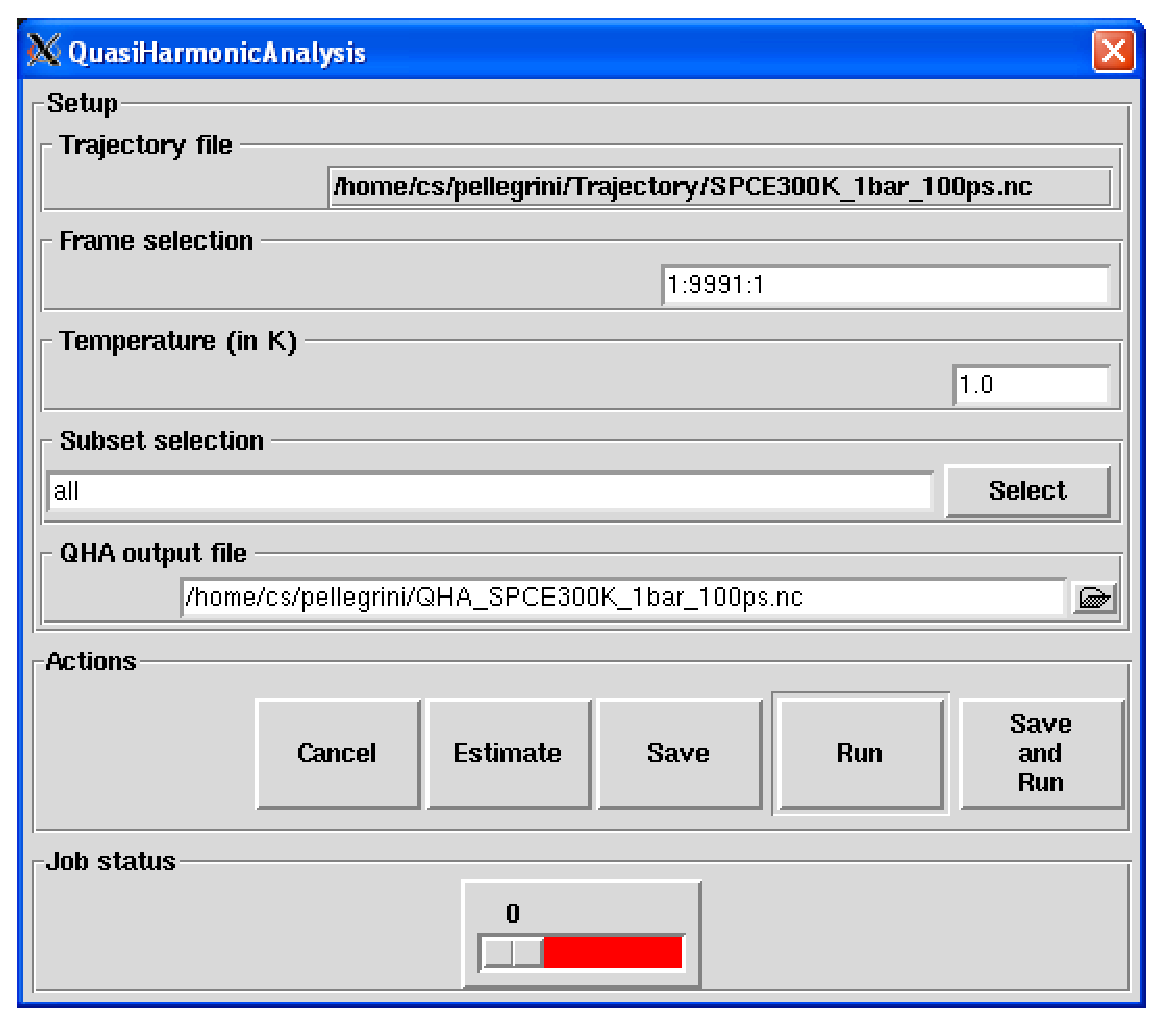
\includegraphics[width=10cm]{Figures/qha.eps}
\end{center}
\caption[The \textit{QHA} analysis dialog]{The dialog from where the \textit{QHA} analysis will be set up and run.}
\label{fig:qha}
\end{figure}   

The following input fields controls the parameters for the \QHA\ analysis:

\begin{itemize}
\item \textbf{Trajectory file}\\
\textbf{Format:} string\\
\textbf{Default:} \textit{traj\_file} where \textit{traj\_file} is the name of the loaded trajectory\\
\textbf{Description:} the value of this widget can not be changed. It just recalls for information purpose the name
of the trajectory file loaded for the analysis.

\item \textbf{Frame selection}\\
\textbf{Format:} string\\
\textbf{Default:} \textit{1:traj\_length:1} where \textit{traj\_length} is the number of frames of the trajectory.\\
\textbf{Description:} this widget allows to select the trajectory frames that will be used for the analysis. This must
be a string of the form:
\\\\
\textit{first:last:step}
\\\\
where \textit{first} is an integer specifying the first frame number to consider, \textit{last} is an integer specifying the last 
frame number to consider and \textit{step} is an integer specifying the step number between two frames.

For example,
\begin{itemize}
\item \textit{2:10:3} will select the frames 2, 5 and 8.
\item \textit{1:5:1} will select the frames 1, 2, 3, 4 and 5.
\end{itemize}

\item \textbf{Temperature (in K)}\\
\textbf{Format:} strictly positive float\\
\textbf{Default:} \textit{1.0}\\
\textbf{Description:} this widget allows to define the temperature factor defined in equation \ref{eq:qha_omega}.

\item \textbf{Subset selection}\\
\textbf{Format:} subset selection string\\
\textbf{Default:} \textit{all}\\
\textbf{Description:} this widget allows the selection of a subset of the system for the analysis. 
See Section \ref{subset_selection} for more details.

\item \textbf{QHA Output file}\\
\textbf{Format:} string\\
\textbf{Default:} \textit{QHA\_traj\_file.nc} where \textit{traj\_file.nc} is the name of the input trajectory\\
\textbf{Description:} this widget allows to enter the name of the \NetCDF\ output file of the \QHA\ analysis.
\end{itemize}

\paragraph{Output\\}
The results of a \QHA\ analysis are stored in a \NetCDF\ file whose main variables are namely:
\begin{itemize}
\item time\_msd: the times in \ps\ at which the \QHA\ was evaluated,
\item omega: the \textit{3N} eigen values $\omega$ defined in equation \ref{eq:qha_omega},
\item dx: a \textit{(3N,3N)} matrix giving the eigen vectors, $\Delta x$ defined in equation \ref{eq:qha_dx}
\item mode: the mode index ranging from 1 to \textit{3N},
\item lci: the local character indicator defined in equation \ref{eq:qha_lci},
\item gci: the global character indicator defined in equation \ref{eq:qha_gci},
\item at: a $(N_{frames},3N)$ matrix where $N_{frames}$ is the number of selected frames for the analysis. This matrix stores 
the projection of \MD\ trajectory onto normal modes as defined in equation \ref{eq:qha_at},
\item{avgstruct: a \textit{(N,3)} matrix storing the averaged structure $\langle x\rangle$}.
\end{itemize}

\subsubsection{Reorientational Correlation Function}
\label{rcf}
\paragraph{Theory and implementation\\}
\label{rcf_theory}
The molecular reorientational correlation function is defined as the conditional probability to find a molecule with 
orientation ${\bf\Omega}_1$ at time $t_1$, given it had the orientation ${\bf\Omega}_0$ at time $t_0$.  In the following 
this probability will be denoted by $p({\bf\Omega}_1,t_1|{\bf\Omega}_0,t_0)$.  Here ${\bf\Omega}$ denotes a set of angular 
coordinates, as Euler angles or quaternion parameters. The joint probability $p({\bf\Omega}_1,t_1;{\bf\Omega}_0,t_0)$ which 
gives the probablity to find a molecule with orientation ${\bf\Omega}_0$ at time $t_0$ and with orientation ${\bf\Omega}_1$ 
at time $t_1$, can be expressed as 
$p({\bf\Omega}_1,t_1;{\bf\Omega}_0,t_0) = p({\bf\Omega}_1,t_1|{\bf\Omega}_0,t_0)\cdot p({\bf\Omega}_0,t_0)$.
Here $p({\bf\Omega}_0,t_0)$ is the probability to find a molecule with orientation ${\bf\Omega}_0$ at time $t_0$. If we 
consider an isotropic system in thermal equilibrium the reorientational correlation function depends only on the time 
{\em difference}, $t = t_1-t_0$, and the {\em change} in orientation, ${\bf\Omega}$, i.e. 
$p({\bf\Omega}_1,t_1|{\bf\Omega}_0,t_0) = p({\bf\Omega},t|{\bf 0},0)$. In addition we have 
$p({\bf\Omega}_0,t_0) = 1/(8\pi^2)$, where $8\pi^2$ is the volume of the angular space.

The reorientational correlation function may now be expanded in Wigner rotation matrices \cite{Stone} which form a complete 
set of basis functions in ${\bf\Omega}$ \cite{Edmonds,Satchler}:
\begin{equation}
\label{eq:p_expansion}
p({\bf\Omega},t|{\bf 0},0) = \sum_{j m n}  \frac{2j +
1}{8\pi^2}\,p^j_{m n}(t) D^{*\,j}_{m n}({\bf \Omega}).
\end{equation}
In the following the coefficients $p^j_{m n}(t)$ are called p-coefficients. Using the orthogonality of the Wigner functions,
\begin{equation}
\label{eq:d_ortho}
\int d\Omega\,D^{*\,j}_{m n}({\bf \Omega})D^{j'}_{m' n'}({\bf \Omega})
= \frac{8\pi^2}{2j + 1}\delta_{jj'}\delta_{mm'}\delta_{nn'},
\end{equation}
Eq. (\ref{eq:p_expansion}) can be inverted to give:
\begin{equation}
\label{eq:p_coeff_p}
p^j_{m n}(t) = \int d\Omega\,p({\bf\Omega},t|{\bf 0},0)
D^{j}_{m n}({\bf \Omega}).
\end{equation}
Writing the reorientational correlation function as
\begin{equation}
p({\bf\Omega},t|{\bf 0},0) = \frac{1}{N}
\sum_\alpha \langle\delta[{\bf\Omega} - {\bf\Omega}_\alpha(t)]\rangle,
\end{equation}
where ${\bf\Omega}_\alpha(t)$ is the orientation of molecule $\alpha$ with respect to its initial orientation and 
$\langle\ldots\rangle$ is a thermal average, relation (\ref{eq:p_coeff_p}) can be written as
\begin{equation}
p^j_{m n}(t) =  \frac{1}{N}
\sum_\alpha \langle D^{j}_{m n}({\bf\Omega}_\alpha(t))\rangle.
\end{equation}
The p-coefficients can also be expressed as time correlation functions of irreducible tensor components. This is convenient 
for numerical purposes since time correlation functions of discrete and finite time series can be very efficiently computed 
by Fast Fourier Transform techniques (see Section \ref{fca}). Consider the general form of the time correlation function
\begin{equation}
\label{eq:tt_t_correl}
\langle T^j_m(t_1) T^{*\,j}_n(t_0) \rangle =
\int\int d\Omega_1 d\Omega_0\,p({\bf\Omega}_1,t_1;{\bf\Omega}_0,t_0)
T^j_m({\bf\Omega}_1)T^{*\,j}_n({\bf\Omega}_0),
\end{equation}
where $T^j_m$ are the components of an {\em irreducible tensor} \cite{Edmonds,Satchler}. From the transformation properties of
irreducible tensors it follows that
\begin{equation}
T^j_m({\bf\Omega}_1) = \sum_k D^{j}_{m k}({\bf \Omega})
T^j_k({\bf\Omega}_0).
\end{equation}
For an isotropic system in thermal equilibrium we may now write
\begin{equation}
p({\bf\Omega}_1,t_1;{\bf\Omega}_0,t_0) =  
p({\bf\Omega},t|{\bf 0},0)\cdot\frac{1}{8\pi^2}.
\end{equation}
Inserting this in (\ref{eq:tt_t_correl}), performing a change in the integration variables from 
$({\bf\Omega}_1,{\bf\Omega}_0)$ to $({\bf\Omega},{\bf\Omega}_0)$, and using the orthogonality of the Wigner functions one 
can show that
\begin{equation}
\label{eq:p_tt}
\langle T^j_m(t) T^{*\,j}_n(0) \rangle =
p^j_{m n}(t) \cdot \frac{1}{2j + 1} \sum_{l}|\hat T^j_l|^2,
\end{equation}
where the components $\hat T^j_l$ are referred to a convenient reference frame. In practice only tensors with integer $j$  
are relevant. In this case, the well known spherical harmonics  \cite{Edmonds,Satchler} may be used to define irreducible tensors.
They are related to the Wigner functions by
\begin{equation}
\label{eq:y_d}
Y^j_m(\alpha,\beta) = \sqrt{\frac{2j+1}{4\pi}}
D^j_{m 0}(\alpha,\beta,\gamma),
\end{equation}
where $\alpha,\beta,\gamma$ are Euler angles. Following {\sc Rose} \cite{Rose} the Wigner functions can be expressed  as 
complex polynomials in the quaternion parameters:
\begin{equation}
\label{eq:wig_q}
\begin{array}{ll}
 &D^{j}_{m n}({\bf q}) = 
        \sum_{p}(-1)^{p}
        \frac{\left[(j+m)!(j-m)!(j+n)!(j-n)!\right]^{1/2}}
             {(j+m-p)!(j-n-p)!p!(p+n-m)!}\\
  &\\
  &\qquad\times (q_0+iq_3)^{j+m-p}(q_0-iq_3)^{j-n-p}
   (q_2+iq_1)^{p+n-m}(q_2-iq_1)^{p}.
\end{array}
\end{equation}
Here the quaternion parameters describe the rotation of the space-fixed coordinate system into the body-fixed coordinate 
system. The corresponding rotation matrix is given in Eq.  (\ref{eq:d_quat}). According to Eq.  (\ref{eq:y_d}) the spherical 
harmonics are just special cases of the Wigner functions,
\begin{equation}
\label{eq:y_q}
\begin{array}{ll}
 &Y^j_m({\bf q}) = \sqrt{\frac{2j+1}{4\pi}} 
        \sum_{p}(-1)^{p}
        \frac{\left[(j+m)!(j-m)!\right]^{1/2} j!}
             {(j+m-p)!(j-p)!p!(j-m)!}\\
  &\\  &\qquad\times(q_0+iq_3)^{j+m-p}(q_0-iq_3)^{j-p}
   (q_2+iq_1)^{p-m}(q_2-iq_1)^{p}.
\end{array}
\end{equation}
Using the normalization of the spherical harmonics  and Eq.
(\ref{eq:p_tt}) one arrives at the following expression
for the p-coefficients
\begin{equation}
\label{p_jmn_y}
p^j_{m n}(t) = 4\pi \langle Y^j_m[{\bf q}(t)]Y^{* j}_n[{\bf q}(0)]\rangle.
\end{equation}
The following relations for the p-coefficients hold:
\begin{eqnarray}
\label{eq:p_initial}
p^j_{m n}(0)     &= &\delta^j_{mn},\\
\label{eq:p_cc}
p^{* j}_{m n}(t) &= &p^{j}_{-m -n}(t) = p^j_{n m}(-t).
\end{eqnarray}
The coefficients $\delta^j_{mn}$ are the components of the $(2j + 1)\times(2j + 1)$ unit matrix. The initial value of the 
the p-coefficients is an immediate consequence of definition (\ref{eq:p_coeff_p}) and 
$p({\bf\Omega},0|{\bf 0},0) = \delta({\bf\Omega})$. Eq. (\ref{eq:p_cc}) follows from the symmetry of the Wigner functions 
and the symmetry of classical time correlation functions. 

Since measurable quantities must be real it follows from (\ref{eq:p_cc}) that only p-coefficients with $m = n = 0$ can be
directly measured. $p^1_{0 0}(t)$ is measured by infrared spectroscopy (dipole-dipole correlation function) and 
$p^2_{0 0}(t)$ by relaxation NMR experiments. Here one measures in most cases the integral over $p^2_{0 0}(t)$.
\newpage
\paragraph{Parameters\\}
\label{rcf_parameters}
Pressing the \textbf{Reorientational Correlation Function} button will pop up the dialog shown on figure \ref{fig:rcf}
\begin{figure}[h!]
\begin{center}
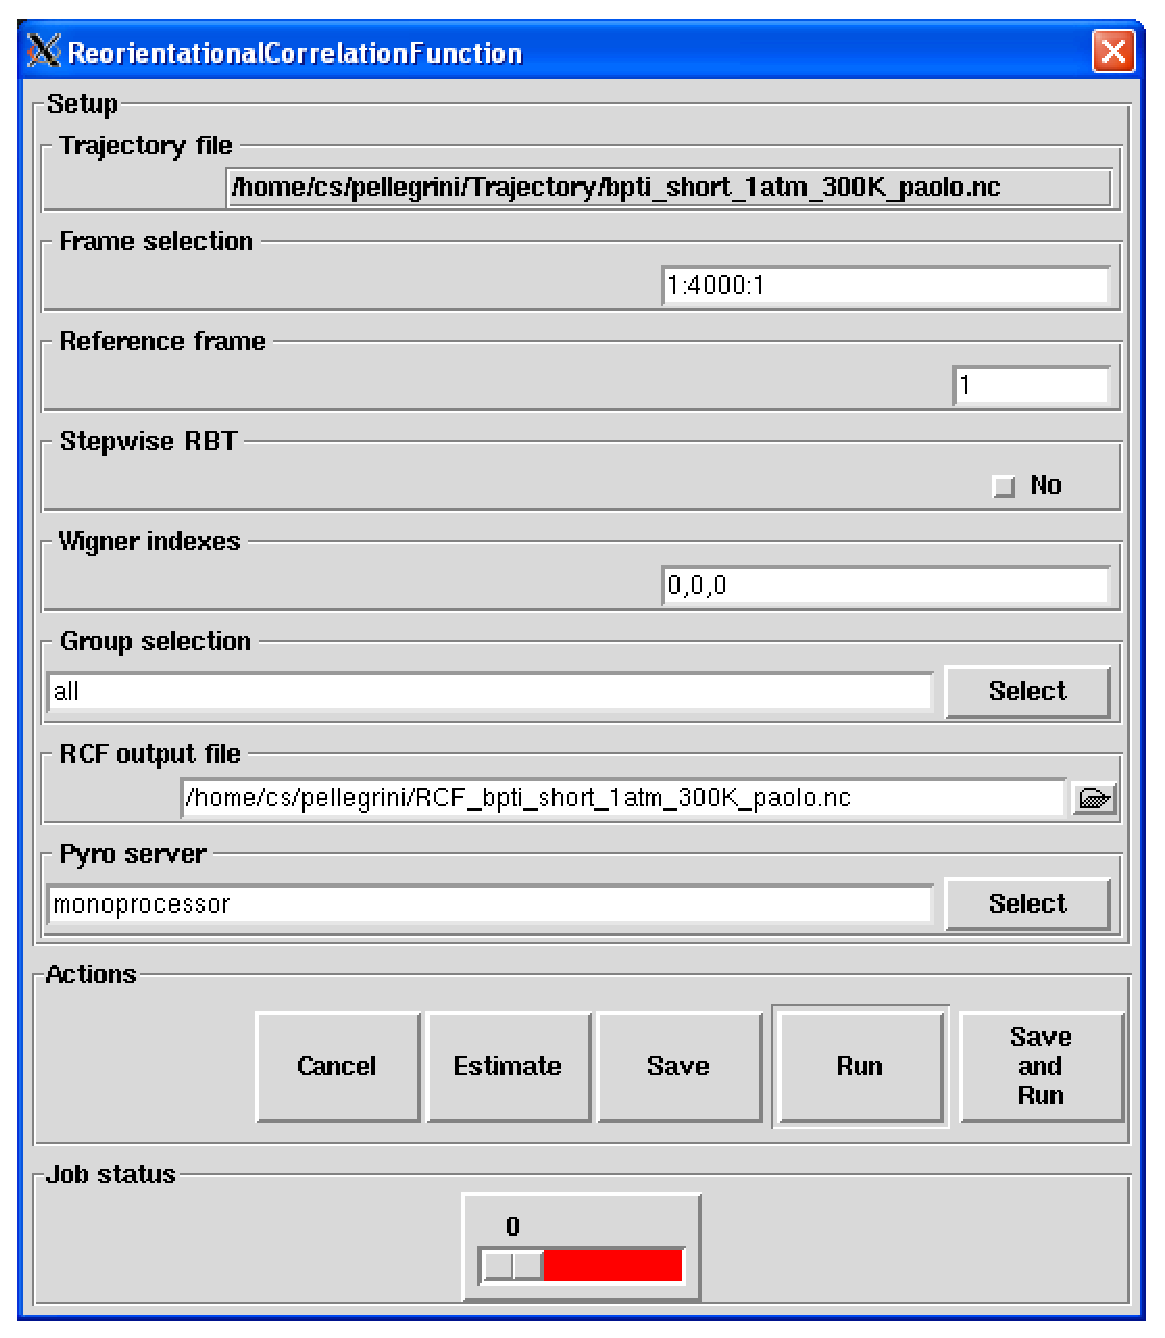
\includegraphics[width=10cm]{Figures/rcf.eps}
\end{center}
\caption[The \textit{RCF} analysis dialog]{The dialog from where the \textit{RCF} analysis will be set up and run.}
\label{fig:rcf}
\end{figure}   

The following input fields controls the parameters for the \RCF\ analysis:

\begin{itemize}
\item \textbf{Trajectory file}\\
\textbf{Format:} string\\
\textbf{Default:} \textit{traj\_file} where \textit{traj\_file} is the name of the loaded trajectory\\
\textbf{Description:} the value of this widget can not be changed. It just recalls for information purpose the name
of the trajectory file loaded for the analysis.

\item \textbf{Frame selection}\\
\textbf{Format:} string\\
\textbf{Default:} \textit{1:traj\_length:1} where \textit{traj\_length} is the number of frames of the trajectory.\\
\textbf{Description:} this widget allows to select the trajectory frames that will be used for the analysis. This must
be a string of the form:
\\\\
\textit{first:last:step}
\\\\
where \textit{first} is an integer specifying the first frame number to consider, \textit{last} is an integer specifying the last 
frame number to consider and \textit{step} is an integer specifying the step number between two frames.

For example,
\begin{itemize}
\item \textit{2:10:3} will select the frames 2, 5 and 8.
\item \textit{1:5:1} will select the frames 1, 2, 3, 4 and 5.
\end{itemize}

\item \textbf{Reference frame}\\
\textbf{Format:} integer in [1,\textit{traj\_length}] where \textit{traj\_length} is the number of frames of the input trajectory\\
\textbf{Default:} \textit{1}\\
\textbf{Description:} this widget allows to specify which frame should be the reference for the \RCF\ analysis.
The value entered should be an integer ranging from 1 to \textit{traj\_length} where \textit{traj\_length} is the 
number of rames of the input trajectory.

\item \textbf{Stepwise RBT}\\
\textbf{Format:} string equal to \textit{yes} or \textit{no}\\
\textbf{Default:} \textit{no}\\
\textbf{Description:} if set to \textit{yes}, each frame \textit{f} will serve as the reference for the frame \textit{f+1} 
when defining the \RBT\ canceling the value entred in \textbf{Reference frame} entry.

\item \textbf{Wigner indexes}\\
\textbf{Format:} string\\
\textbf{Default:} \textit{0,0,0}\\
\textbf{Description:} this widget allows to specify which Wigner triplet \textit{(j,m,n)} to select for the \RCF\ analysis. 
The entered value must have the following specific format:
\\\\
\textit{j:m:n}
\\\\
where \textit{j}, \textit{m},\textit{n} are positive integers that represent respectively the \textit{j}, \textit{m},\textit{n} Wigner indexes.

\item \textbf{Group selection}\\
\textbf{Format:} group selection string\\
\textbf{Default:} \textit{all}\\
\textbf{Description:} this widget allows the selection of the groups of atoms that will be defined as rigid-bodies when 
performing the \RCF . See Section \ref{group_selection} for more details.

\item \textbf{RCF output file}\\
\textbf{Format:} string\\
\textbf{Default:} \textit{RCF\_traj\_file.nc} where \textit{traj\_file.nc} is the name of the input trajectory\\
\textbf{Description:} this widget allows to enter the name of the \NetCDF\ output file of the \RCF\ analysis. A \CDL\ 
version of the \NetCDF\ output file is also automatically created with \textit{RCF\_traj\_file.cdl} name.
\end{itemize}

\paragraph{Output\\}
The results of a \RCF\ analysis are stored in a \NetCDF\ file whose main variables are namely:
\begin{itemize}
\item time: the times in \ps\ at which the \RCF\ was evaluated,
\item rcf: the corresponding \RCF .
\end{itemize}

\subsubsection{Angular Velocity AutoCorrelation Function}
\label{avacf}
\paragraph{Theory and implementation\\}
\label{avacf_theory}
Similarly to the translational velocity autocorrelation functions introduced in Section \ref{vacf} one can define angular 
velocity autocorrelation functions to characterize the angular motion of molecules. In general the angular velocity is 
referred to an orthonormal {\em body-fixed} coordinate system. Usually this is the principal axis system in which the tensor 
of inertia is diagonal. Depending on its geometry, a molecule will behave differently with respect to rotational motion 
about different body-fixed axes.  The autocorrelation function for the angular velocity components $\omega'_{i}$ is defined 
as
\begin{equation}
\label{eq:c_omgomg}
C_{\omega\omega}(t;i) \doteq
\langle\omega'_{i}(0)\omega_{i}'(t) \rangle.
\end{equation}
The prime indicates a body fixed coordinate system. The components $\omega'_{i}$ are related to the quaternion parameters
describing the orientation of the molecule and their time derivatives \cite{Smith:1992,Tildesley}:
\begin{equation}
\label{eq:omega_prime_quat_dot)}
\left(\begin{array}{c}
      0         \\
      \omega'_x \\
      \omega'_y \\
      \omega'_z 
      \end{array}
\right)      
      = 2 \cdot
\left(
\begin{array}{rrrr}
  q_0 & q_1 & q_2 & q_3 \\
 -q_1 & q_0 & q_3 &-q_2 \\
 -q_2 &-q_3 & q_0 & q_1 \\
 -q_3 & q_2 &-q_1 & q_0 
\end{array}
\right)
\left(\begin{array}{c}
      \dot q_0 \\
      \dot q_1 \\
      \dot q_2 \\
      \dot q_3 
      \end{array}
\right).
\end{equation}
Here the quaternion parameters describe the rotation of the space-fixed coordinate system into the body-fixed coordinate 
system. The corresponding rotation matrix is explicitly given in Eq. (\ref{eq:d_quat}).

The components of the angular velocity may be used to define rotation angles describing rotations about the body-fixed axes
\cite{Smith:1992}:
\begin{equation}
\label{phi_omega}
\Phi_i(t) = \int_0^t d\tau\,\omega'_i(\tau).
\end{equation}

\paragraph{Parameters\\}
\label{avacf_parameters}
Pressing the \textbf{Angular Velocity Autocorrelation Function} button will pop up the dialog shown on figure \ref{fig:avacf}
\begin{figure}[h!]
\begin{center}
\includegraphics[width=10cm]{Figures/avacf.eps}
\end{center}
\caption[The \textit{AVACF} analysis dialog]{The dialog from where the \textit{AVACF} analysis will be set up and run.}
\label{fig:avacf}
\end{figure}   

The following input fields controls the parameters for the \AVACF\ analysis:

\begin{itemize}
\item \textbf{Trajectory file}\\
\textbf{Format:} string\\
\textbf{Default:} \textit{traj\_file} where \textit{traj\_file} is the name of the loaded trajectory\\
\textbf{Description:} the value of this widget can not be changed. It just recalls for information purpose the name
of the trajectory file loaded for the analysis.

\item \textbf{Frame selection}\\
\textbf{Format:} string\\
\textbf{Default:} \textit{1:traj\_length:1} where \textit{traj\_length} is the number of frames of the trajectory.\\
\textbf{Description:} this widget allows to select the trajectory frames that will be used for the analysis. This must
be a string of the form:
\\\\
\textit{first:last:step}
\\\\
where \textit{first} is an integer specifying the first frame number to consider, \textit{last} is an integer specifying the last 
frame number to consider and \textit{step} is an integer specifying the step number between two frames.

For example,
\begin{itemize}
\item \textit{2:10:3} will select the frames 2, 5 and 8.
\item \textit{1:5:1} will select the frames 1, 2, 3, 4 and 5.
\end{itemize}

\item \textbf{Differentiation order}\\
\textbf{Format:} integer in [0,5]\\
\textbf{Default:} 0 if velocities are stored in the trajectory file, 1 otherwise\\
\textbf{Description:} this widget allows to specify the order of the derivation scheme used to get the velocities out 
of the coordinates. If your trajectory \NetCDF\ file already contains the velocities then just select \textit{0}.
However, you can still decide to get the velocities out of the coordinates. In that case, \NMOLDYN\ performs a numerical 
differentiation of the input data. To do so, \NMOLDYN\ can perform numerical differentiation from order \textit{1} to 
order \textit{5}. Using order \textit{1}, the first time derivative of each point $r(t_i)$ 
is calculated as
\begin{equation}
\dot{r}(t_i)=\frac{r(t_{i+1})-r(t_{i})} {\Delta t},
\end{equation}
where $\Delta t$ is the time step. 
Choosing order \textit{N} with \textit{N=2,...,5}, \NMOLDYN\ calculates the first time-derivative of each point 
$r(t_i)$ ($r=x,y,z$) using the \textit{N}-order polynomial interpolating the \textit{N+1} points across $r(t_i)$, where $r(t_i)$ 
belongs to this set \cite{Abramowitz}.

\item \textbf{Project displacement on}\\
\textbf{Format:} string\\
\textbf{Default:} \textit{no}\\
\textbf{Description:} this widget allows to specify a vector along which the \AVACF\ will be computed. This vector does not 
need to be normalized as \NMOLDYN\ will perform the normalization when processing it. The entered value must have the 
following format:
\\\\
\textit{vx:vy:vz}
\\\\
where \textit{vx}, \textit{vy} and \textit{vz} are floats that represent respectively the \textit{x}, \textit{y} and \textit{z} coordinates of the vector.

\item \textbf{Reference frame}\\
\textbf{Format:} integer in [1,\textit{traj\_length}] where \textit{traj\_length} is the number of frames of the input trajectory\\
\textbf{Default:} \textit{1}\\
\textbf{Description:} this widget allows to specify which frame should be the reference for the \AVACF\ analysis.
The value entered should be an integer ranging from 1 to \textit{traj\_length} where \textit{traj\_length} is the 
number of rames of the input trajectory.

\item \textbf{Stepwise RBT}\\
\textbf{Format:} string equal to \textit{yes} or \textit{no}\\
\textbf{Default:} \textit{no}\\
\textbf{Description:} if set to \textit{yes}, each frame \textit{f} will serve as the reference for the frame \textit{f+1} 
when defining the \RBT\ canceling the value entred in \textbf{Reference frame} entry.

\item \textbf{Group selection}\\
\textbf{Format:} group selection string\\
\textbf{Default:} \textit{all}\\
\textbf{Description:} this widget allows the selection of the groups of atoms that will be defined as rigid-bodies 
when performing the \AVACF . See Section \ref{group_selection} for more details.

\item \textbf{AVACF output file}\\
\textbf{Format:} string\\
\textbf{Default:} \textit{AVACF\_traj\_file.nc} where \textit{traj\_file.nc} is the name of the input trajectory\\
\textbf{Description:} this widget allows to enter the name of the \NetCDF\ output file of the \AVACF\ analysis. A \CDL\ 
version of the \NetCDF\ output file is also automatically created with \textit{AVACF\_traj\_file.cdl} name.
\end{itemize}

\paragraph{Output\\}
The results of a \AVACF\ analysis are stored in a \NetCDF\ file whose main variables are namely:
\begin{itemize}
\item time: the times in \ps\ at which the \AVACF\ was evaluated,
\item avacf: the corresponding \AVACF.
\end{itemize}

\subsubsection{Angular Density Of States}
\label{ados}
\paragraph{Theory and implementation\\}
\label{ados_theory}
In \textit{n}MOLDYN, the \ADOS\ is simply defined as the Fourier transform of the \AVACF .

\paragraph{Parameters\\}
\label{ados_parameters}
Pressing the \textbf{Angular Density Of States} button will pop up the dialog shown on figure \ref{fig:ados}
\begin{figure}[h!]
\begin{center}
\includegraphics[width=10cm]{Figures/ados.eps}
\end{center}
\caption[The \textit{ADOS} analysis dialog]{The dialog from where the \textit{ADOS} analysis will be set up and run.}
\label{fig:ados}
\end{figure}   

The following input fields controls the parameters for the \ADOS\ analysis:

\begin{itemize}
\item \textbf{Trajectory file}\\
\textbf{Format:} string\\
\textbf{Default:} \textit{traj\_file} where \textit{traj\_file} is the name of the loaded trajectory\\
\textbf{Description:} the value of this widget can not be changed. It just recalls for information purpose the name
of the trajectory file loaded for the analysis.

\item \textbf{Frame selection}\\
\textbf{Format:} string\\
\textbf{Default:} \textit{1:traj\_length:1} where \textit{traj\_length} is the number of frames of the trajectory.\\
\textbf{Description:} this widget allows to select the trajectory frames that will be used for the analysis. This must
be a string of the form:
\\\\
\textit{first:last:step}
\\\\
where \textit{first} is an integer specifying the first frame number to consider, \textit{last} is an integer specifying the last 
frame number to consider and \textit{step} is an integer specifying the step number between two frames.

For example,
\begin{itemize}
\item \textit{2:10:3} will select the frames 2, 5 and 8.
\item \textit{1:5:1} will select the frames 1, 2, 3, 4 and 5.
\end{itemize}

\item \textbf{Differentiation order}\\
\textbf{Format:} integer in [0,5]\\
\textbf{Default:} 0 if velocities are stored in the trajectory file, 1 otherwise\\
\textbf{Description:} this widget allows to specify the order of the derivation scheme used to get the velocities out 
of the coordinates. If your trajectory \NetCDF\ file already contains the velocities then just select \textit{0}.
However, you can still decide to get the velocities out of the coordinates. In that case, \NMOLDYN\ performs a numerical 
differentiation of the input data. To do so, \NMOLDYN\ can perform numerical differentiation from order \textit{1} to 
order \textit{5}. Using order \textit{1}, the first time derivative of each point $r(t_i)$ 
is calculated as
\begin{equation}
\dot{r}(t_i)=\frac{r(t_{i+1})-r(t_{i})} {\Delta t},
\end{equation}
where $\Delta t$ is the time step. 
Choosing order \textit{N} with \textit{N=2,...,5}, \NMOLDYN\ calculates the first time-derivative of each point 
$r(t_i)$ ($r=x,y,z$) using the \textit{N}-order polynomial interpolating the \textit{N+1} points across $r(t_i)$, where $r(t_i)$ 
belongs to this set \cite{Abramowitz}.

\item \textbf{Project displacement on}\\
\textbf{Format:} string\\
\textbf{Default:} \textit{no}\\
\textbf{Description:} this widget allows to specify a vector along which the \ADOS\ will be computed. This vector does not 
need to be normalized as \NMOLDYN\ will perform the normalization when processing it. The entered value must have the 
following format:
\\\\
\textit{vx:vy:vz}
\\\\
where \textit{vx}, \textit{vy} and \textit{vz} are floats that represent respectively the \textit{x}, \textit{y} and \textit{z} coordinates of the vector.

\item \textbf{Reference frame}\\
\textbf{Format:} integer in [1,\textit{traj\_length}] where \textit{traj\_length} is the number of frames of the input trajectory\\
\textbf{Default:} \textit{1}\\
\textbf{Description:} this widget allows to specify which frame should be the reference for the \ADOS\ analysis.
The value entered should be an integer ranging from 1 to \textit{traj\_length} where \textit{traj\_length} is the 
number of rames of the input trajectory.

\item \textbf{Stepwise RBT}\\
\textbf{Format:} string equal to \textit{yes} or \textit{no}\\
\textbf{Default:} \textit{no}\\
\textbf{Description:} if set to \textit{yes}, each frame \textit{f} will serve as the reference for the frame \textit{f+1} 
when defining the \RBT\ canceling the value entred in \textbf{Reference frame} entry.

\item \textbf{FFT window}\\
\textbf{Format:} float in [0.0,100.0]\\
\textbf{Default:} \textit{10.0}\\
\textbf{Description:} this widget allows to define the width in percentage of the trajectory length of the Gaussian 
function to be used in the smoothing procedure for the calculation of the \ADOS . See Appendix \ref{fca} for more details.

\item \textbf{Group selection}\\
\textbf{Format:} group selection string\\
\textbf{Default:} \textit{all}\\
\textbf{Description:} this widget allows the selection of the groups of atoms that will be defined as rigid-bodies 
when performing the \ADOS . See Section \ref{group_selection} for more details.

\item \textbf{ADOS output file}\\
\textbf{Format:} string\\
\textbf{Default:} \textit{ADOS\_traj\_file.nc} where \textit{traj\_file.nc} is the name of the input trajectory\\
\textbf{Description:} this widget allows to enter the name of the \NetCDF\ output file of the \ADOS\ analysis. A \CDL\ 
version of the \NetCDF\ output file is also automatically created with \textit{ADOS\_traj\_file.cdl} name.
\end{itemize}

\paragraph{Output\\}
The results of a \ADOS\ analysis are stored in a \NetCDF\ file whose main variables are namely:
\begin{itemize}
\item frequency: the frequencies in \thz\ at which the \ADOS\ was evaluated,
\item ados: the corresponding \ADOS .
\end{itemize}

\subsection{The Scattering menu}
\label{scattering_menu}
Pressing the button \textbf{Scattering} brings up a menu from which it is possible to choose the following analysis:
\begin{itemize}
\item Dynamic Coherent Structure Factor
\item Dynamic Coherent Structure Factor (AR Model)
\item Dynamic Incoherent Structure Factor
\item Dynamic Incoherent Structure Factor (AR Model)
\item Dynamic Incoherent Structure Factor (Gaussian Approximation)
\item Elastic Incoherent Structure Factor
\item Static Coherent Structure Factor
\item Smoothed Static Coherent Structure Factor
\end{itemize}
Before introducing each of these analysis, a brief introduction about the scattering theory within the classical framework will be given.

\subsubsection{Introduction\\}
\label{scattering_introduction}
The quantity of interest in neutron scattering experiments with thermal neutrons is the {\em dynamic structure factor}, 
${\cal S}({\bf q},\omega)$, which is closely related to the double differential cross-section \cite{Lovesey}, 
$d^2\sigma/d\Omega dE$.  The double differential cross section is defined as the number of neutrons which
are scattered per unit time into the solid angle interval $[\Omega,\Omega+d\Omega]$ and into the energy interval \textit{[E,E+dE]}. 
It is normalized to $d\Omega$, \textit{dE}, and the flux of the incoming neutrons,
\begin{equation}
\label{eq:sqw_1}
\frac{d^{2}\sigma}{d\Omega dE} = N\cdot\frac{k}{k_0}{\cal S}({\bf q},\omega).
\end{equation}
Here \textit{N} is the number of atoms, and $k\equiv|{\bf k}|$  and $k_0\equiv |{\bf k}_0|$ are the wave numbers of scattered and 
incident neutrons, respectively. They are related to the corresponding neutron energies by 
$E = \hbar^2 k^2/2m$ and $E_0 = \hbar^2 k_0^2/2m$, where $m$ is the neutron mass. The arguments of the dynamic structure 
factor, \textit{\textbf{q}} and $\omega$, are the momentum and energy transfer in units of $\hbar$, respectively:
\begin{eqnarray}
{\bf q} &= &\frac{{\bf k}_0 - {\bf k}}{\hbar},\\
\omega  &= &\frac{E_0 - E}{\hbar}.
\end{eqnarray}
The modulus of the momentum transfer can be expressed in the scattering angle $\theta$, the energy transfer, and the energy of 
the incident neutrons:
\begin{equation}
q = \sqrt{2 - \frac{\hbar\omega}{E_0} 
          - 2\cos\theta\sqrt{2 - \frac{\hbar\omega}{E_0}}}.
\end{equation}
The dynamic structure factor contains information about the structure and dynamics of the scattering system \cite{VanHove}.
It can be written as 
\begin{equation}
\label{eq:sqw_2}
{\cal S}({\bf q},\omega) = \frac{1}{2\pi}\int_{-\infty}^{+\infty}dt\, \exp[-i\omega t]{\cal F}({\bf q},t).
\end{equation}
${\cal F}({\bf q},t)$ is called the {\em intermediate scattering function} and is defined as
\begin{eqnarray}
\label{eq:fqt}
{\cal F}({\bf q},t) &= &\sum_{\alpha,\beta}\Gamma_{\alpha\beta}
\langle\exp[-i{\bf q}\cdot\hat{\bf R}_\alpha(0)]
       \exp[i{\bf q}\cdot\hat{\bf R}_\beta(t)]\rangle,\\
\label{eq:gamma}
\Gamma_{\alpha\beta} &= &\frac{1}{N}
\left[\overline{\mbox{$b_\alpha$}}\,\overline{\mbox{$b_\beta$}} 
+ \delta_{\alpha\beta}
 (\overline{b_\alpha^{\,2}} - \overline{b_\alpha}^{\,2})\right].
\end{eqnarray}
The operators $\hat {\bf R}_\alpha(t)$ in Eq. (\ref{eq:fqt}) are the position operators of the nuclei in the sample. 
The brackets $\langle\ldots\rangle$ denote a quantum thermal average and the time dependence of the position operators 
is defined by the Heisenberg picture.  The quantities $b_\alpha$ are the scattering lengths of the nuclei which depend 
on the isotope and the relative orientation of the spin of the neutron and the spin of the scattering nucleus. If the
spins of the nuclei and the neutron are not prepared in a special orientation one can assume a random relative orientation 
and that spin and position of the nuclei are uncorrelated. The symbol 
$\overline{\rule{0pt}{5pt}\ldots}$ appearing in $\Gamma_{\alpha\beta}$ denotes an average over isotopes and relative spin 
orientations of neutron and nucleus.

Usually one splits the intermediate scattering function and the dynamic structure factor into their {\em coherent} and 
{\em incoherent} parts which describe collective and single particle motions, respectively.
Defining
\begin{eqnarray}
b_{\alpha,coh} &\doteq &\overline{b_\alpha},\\ b_{\alpha,inc} &\doteq
&\sqrt{ \overline{b_\alpha^{\,2}} - \overline{b_\alpha}^{\,2} },
\end{eqnarray}
the coherent and incoherent intermediate scattering functions can be cast in the form
\begin{eqnarray}
{\cal F}_{coh}({\bf q},t) &= &\frac{1}{N}\sum_{\alpha,\beta}
b_{\alpha,coh}\,b_{\beta,coh}
\langle\exp[-i{\bf q}\cdot\hat{\bf R}_\alpha(0)]
       \exp[i{\bf q}\cdot\hat{\bf R}_\beta(t)]\rangle,\\
{\cal F}_{inc}({\bf q},t) &= &\frac{1}{N}\sum_{\alpha}
b_{\alpha,inc}^{\,2}
\langle\exp[-i{\bf q}\cdot\hat{\bf R}_\alpha(0)]
       \exp[i{\bf q}\cdot\hat{\bf R}_\alpha(t)]\rangle.
\end{eqnarray}
Rewriting these formulas, \NMOLDYN\ introduces the partial terms as:
\begin{eqnarray}
\label{eq:fcoh}
{\cal F}_{\mathrm{coh}}({\bf q},t) &= & \sum^{N_{species}}_{I,J \ge I}\sqrt{n_I n_J\omega_{I,\mathrm{coh}}\omega_{J,\mathrm{coh}}}{\cal F}_{IJ,\mathrm{coh}}({\bf q},t),\\
\label{eq:finc}
{\cal F}_{\mathrm{inc}}({\bf q},t) &= &\sum^{N_{species}}_{I = 1}n_I \omega_{I,\mathrm{inc}}{\cal F}_{I,\mathrm{inc}}({\bf q},t)
\end{eqnarray}
where:
\begin{eqnarray}
{\cal F}_{IJ,\mathrm{coh}}({\bf q},t) &= &\frac{1}{\sqrt{n_In_J}}\sum^{n_I}_{\alpha}\sum^{n_J}_{\beta}
\langle\exp[-i{\bf q}\cdot\hat{\bf R}_\alpha(t_0)]
       \exp[i{\bf q}\cdot\hat{\bf R}_\beta(t_0+t)]\rangle_{t_0},\\
{\cal F}_{I,\mathrm{inc}}({\bf q},t) &= & \frac{1}{n_I}\sum^{n_I}_{\alpha = 1}\langle\exp[-i{\bf q}
\cdot\hat{\bf R}_\alpha(t_0)]\exp[i{\bf q}\cdot\hat{\bf R}_\alpha(t_0+t)]\rangle_{t_0}.
\end{eqnarray}
where $n_I$, $n_J$, $N_{species}$, $\omega_{I,\mathrm{coh,inc}}$ and $\omega_{J,\mathrm{coh,inc}}$ are defined in 
Section \ref{weighting_scheme}.

The corresponding dynamic structure factors are obtained by performing the Fourier transformation defined in 
Eq. \ref{eq:sqw_2}.

An important quantity describing {\em structural} properties of liquids is the {\em static structure factor}, which 
is defined as
\begin{equation}
\label{eq:sq}
{\cal S}({\bf q}) \doteq \int_{-\infty}^{+\infty}d\omega\,
{\cal S}_{coh}(q,\omega) = {\cal F}_{coh}({\bf q},0).
\end{equation}

In the classical framework the intermediate scattering functions are interpreted as classical time correlation functions. 
The position operators are replaced by time-dependent vector functions and quantum thermal averages are replaced by classical 
{\em ensemble averages}. It is well known that this procedure leads to a loss of the universal detailed balance relation,
\begin{equation}
\label{eq:detbal}
{\cal S}({\bf q},\omega) = \exp[\beta\hbar\omega]
{\cal S}(-{\bf q},-\omega),
\end{equation}
and also to a loss of all odd moments
\begin{equation}
\label{eq:moments}
\langle\omega^{2n+1}\rangle \doteq
\int_{-\infty}^{+\infty}d\omega\,\omega^{2n+1} {\cal S}({\bf
q},\omega), \qquad n = 1,2,\ldots.
\end{equation}
The odd moments vanish since the classical dynamic structure factor is even in $\omega$, assuming invariance of the scattering 
process with respect to reflections in space. The first moment is also universal. For an atomic liquid, containing only one 
sort of atoms, it reads
\begin{equation}
\label{eq:recoil}
\langle\omega\rangle = \frac{\hbar q^2}{2M}\:,
\end{equation} 
where $M$ is the mass of the atoms.  Formula (\ref{eq:recoil}) shows that the first moment is given by the average kinetic 
energy (in units of $\hbar$) of a particle  which receives a momentum transfer 
$\hbar {\bf q}$. Therefore $\langle\omega\rangle$ is called  the {\em recoil moment}. A number of `recipes' has been 
suggested to correct classical dynamic structure factors for detailed balance and to describe recoil effects in an 
approximate way. The most popular one has been suggested by Schofield \cite{Schofield}
\begin{equation}
\label{eq:detbal_corr}
{\cal S}({\bf q},\omega) \approx
\exp[\frac{\beta\hbar\omega}{2}]{\cal S}_{cl}({\bf q},\omega).
\end{equation}
One can easily verify that the resulting dynamic structure factor fulfills the relation of detailed balance. Formally, the 
correction (\ref{eq:detbal_corr}) is correct to first order in $\hbar$. Therefore it cannot be used for large \qval-values which 
correspond to large momentum transfers  $\hbar q$. This is actually true for all correction methods which have suggested so far. 
For more details we refer to Ref. \cite{Kneller:1994}.

\subsubsection{Dynamic Coherent Structure Factor}
\label{dcsf}
\paragraph{Theory and implementation\\}
\label{dcsf_theory}
Please refer to Section \ref{scattering_introduction} for more details about the theoretical background related to the dynamic 
coherent structure factor. In this analysis, \NMOLDYN\ proceeds in two steps. First, it computes the partial and total 
intermediate coherent scattering function using equation \ref{eq:fcoh}. Then, the partial and total dynamic coherent 
structure factors are obtained by performing the Fourier Transformation, defined in Eq. \ref{eq:sqw_2}, respectively on 
the total and partial intermediate coherent scattering functions.

\NMOLDYN\ computes the coherent intermediate scattering function on a rectangular grid of equidistantly spaced points along 
the time-and the \qval-axis, repectively:
\begin{equation} 
\label{eq:fqt_coh_num}
{\cal F}_{\mathrm{coh}}(q_m,k\cdot\Delta t) \doteq \sum^{N_{species}}_{I=1,J\ge I} \sqrt{n_I n_J \omega_{I,\mathrm{com}}\omega_{I,\mathrm{com}}}
\overline{\langle \rho_I(-{\bf q},0)\rho_J({\bf q},k\cdot\Delta t) \rangle}^{q},
\qquad k = 0\ldots N_t - 1,\; m = 0\ldots N_q - 1. 
\end{equation} 
where $N_t$ is the number of time steps in the coordinate time series, $N_q$ is a user-defined number of \qshells, 
$N_{species}$ is the number of selected species, $n_I$ the number of atoms of species \textit{I}, $\omega_I$ the weight for specie 
\textit{I} (see Section \ref{weighting_scheme} for more details) and $\rho_I({\bf q},k\cdot\Delta t)$ is the Fourier transformed particle 
density for specie \textit{I} defined as,
\begin{equation}
\label{eq:dcsf_rho}
\rho_I({\bf q},k\cdot\Delta t) = \sum_\alpha^{n_I} \exp[i{\bf q}\cdot{\bf R}_\alpha(k\cdot\Delta t)].
\end{equation}
The symbol $\overline{\rule{0pt}{5pt}\ldots}^{q}$ in (\ref{eq:fqt_coh_num}) denotes an average over \qvects\ having 
{\em approximately} the same modulus $q_m = q_{min} + m\cdot\Delta q$. The particle density must not change if jumps in 
the particle trajectories due to periodic boundary conditions occcur. In addition the {\em average} particle density, 
$N/V$, must not change. This can be achieved by choosing \qvects\ on a lattice which is reciprocal to the lattice defined 
by the \MD\ box. Let ${\bf b}_1,{\bf b}_2,{\bf b}_3$ be the basis vectors which span the \MD\ cell. Any position vector in the 
\MD\ cell can be written as
\begin{equation}
{\bf R} = x'{\bf b}_1 + y'{\bf b}_2 + z'{\bf b}_3,
\end{equation}
with $x',y',z'$ having values between $0$ and $1$.  The primes indicate that the coordinates are box coordinates. A jump due 
to periodic bounday conditions causes $x',y',z'$ to jump by $\pm 1$.  The set of dual basis vectors ${\bf b}^1,{\bf b}^2,{\bf b}^3$ 
is defined by the relation
\begin{equation}
{\bf b}_i{\bf b}^j = \delta_i^j.
\end{equation}
If the \qvects\ are now chosen as
\begin{equation}
\label{eq:q_dual}
{\bf q} = 2\pi\left(k{\bf b}^1 + l{\bf b}^2 + m{\bf b}^3\right),
\end{equation}
where \textit{k,l,m} are integer numbers, jumps in the particle trajectories produce phase changes of multiples of $2\pi$ in the 
Fourier transformed particle density, i.e. leave it unchanged. One can define a grid of \qshells\ or a grid of \qvects\ 
along a given direction or on a given plane, giving in addition a {\em tolerance} for \qval. \NMOLDYN\ looks then for 
\qvects\ of the form (\ref{eq:q_dual}) whose moduli deviate within the prescribed tolerance from the equidistant \qval-grid. 
From these \qvects\ only a maximum number per grid-point (called generically \qshell\ also in the anisotropic case) is 
kept.

The \qvects\ can be generated isotropically, anisotropically or along user-defined directions.

The $\sqrt{\omega_I}$ may be negative if they represent normalized coherent scattering lenghts, i.e.
\begin{equation}
\sqrt{\omega_I} = \frac{b_{I,\mathrm{coh}}}{\sqrt{\sum_{I = 1}^{N_{species}} n_I b^2_{I,\mathrm{coh}}}}.
\end{equation}
Negative coherent scattering lengths occur in hydrogenous materials since $b_{coh,H}$ is negative \cite{Lovesey}.
The density-density correlation is computed via the \FCA\ technique described in Section \ref{fca}.
\newpage
\paragraph{Parameters\\}
\label{dcsf_parameters}
Pressing the \textbf{Dynamic Coherent Structure Factor} button will pop up the dialog shown on figure \ref{fig:dcsf}
\begin{figure}[h!]
\begin{center}
\includegraphics[width=10cm]{Figures/dcsf.eps}
\end{center}
\caption[The \textit{DCSF} analysis dialog]{The dialog from where the \textit{DCSF} analysis will be set up and run.}
\label{fig:dcsf}
\end{figure}   

The following input fields controls the parameters for the \DCSF\ analysis:

\begin{itemize}
\item \textbf{Trajectory file}\\
\textbf{Format:} string\\
\textbf{Default:} \textit{traj\_file} where \textit{traj\_file} is the name of the loaded trajectory\\
\textbf{Description:} the value of this widget can not be changed. It just recalls for information purpose the name
of the trajectory file loaded for the analysis.

\item \textbf{Frame selection}\\
\textbf{Format:} string\\
\textbf{Default:} \textit{1:traj\_length:1} where \textit{traj\_length} is the number of frames of the trajectory.\\
\textbf{Description:} this widget allows to select the trajectory frames that will be used for the analysis. This must
be a string of the form:
\\\\
\textit{first:last:step}
\\\\
where \textit{first} is an integer specifying the first frame number to consider, \textit{last} is an integer specifying the last 
frame number to consider and \textit{step} is an integer specifying the step number between two frames.

For example,
\begin{itemize}
\item \textit{2:10:3} will select the frames 2, 5 and 8.
\item \textit{1:5:1} will select the frames 1, 2, 3, 4 and 5.
\end{itemize}

\item \textbf{Q values (in nm-1)}\\
\textbf{Format:} string\\
\textbf{Default:} \textit{0:100:1.}\\
\textbf{Description:} this widget allows to select the modulii of the \qvects . This must
be a string of the form:
\\\\
$q_{min}:q_{max}:q_{step}$
\\\\
In this way, the intermediate scattering function will be calculated for discrete \qval\ defined as 
$q_m = q_{min} + m \cdot q_{step}$ where $q_{min}$ is the radius of the smallest \qshell , $q_{step}$ is the 
distance between two consecutive \qshells\ and with \textit{m} running from 0 to $N_{shell}$ where $N_{shell}$ is the 
number of selected \qshells\ defined as $N_{shell}= E(\frac{q_{max} - q_{min}}{q_{step}}) + 1$ where $q_{max}$ is the 
radius of the biggest \qshell .

For example,
\begin{itemize}
\item \textit{0:10:1} will generate \qshells\ of radii 0, 1, 2, 3, 4, 5, 6, 7, 8, 9, 10.
\item \textit{3:12:2} will generate \qshells\ of radii 3, 5, 7, 9, 11.
\end{itemize}

\item \textbf{Q shell width (in nm-1)}\\
\textbf{Format:} strictly positive float\\
\textbf{Default:} \textit{1.0}\\
\textbf{Description:} this widget allows to define the tolerance \textit{dq} on the \qval -modulii. So, for each \qshell\ of 
modulus \qval , \NMOLDYN\ will accept a \qvect\ to belong to that shell if its modulus falls in the range 
\textit{[q-dq/2,q+dq/2]}. This parameter fix the \qval -resolution.

\item \textbf{Q vectors per shell}\\
\textbf{Format:} strictly positive integer\\
\textbf{Default:} \textit{50}\\
\textbf{Description:} this widget allows to specify the number of \qvects\ , $N_q$ to generate for each \qshell . Indeed, 
when generating \qvects , \NMOLDYN\ will try to generate $N_q$ \qvects\ for each \qshell\ in order to carry out the averages 
of Eq. \ref{eq:dcsf_rho}. For a given \qshell , if \NMOLDYN\ could generate less \qvects\ than $N_q$, it will only use the 
number of generated \qvects\ instead of $N_q$ and if \NMOLDYN\ could generate more \qvects\ than $N_q$, it will pick up
randomly $N_q$ \qvects\ among the generated \qvects . The higher this parameter is the smoother will be the computed 
intermediate scattering function but at the cost of a slower analysis.

\item \textbf{Q vectors generator}\\
\textbf{Format:} string equal to \textit{3D isotropic}, \textit{2D isotropic} or \textit{anisotropic}\\
\textbf{Default:} \textit{3D isotropic}\\
\textbf{Description:} this option allows to specify how the \qvects\ should be generated:
\begin{itemize}
\item{3D isotropic} the \qvects\ are generated randomly on concentric spheres.
\item{2D isotropic} the \qvects\ are generated randomly on concentric rings in a given plane.
\item{anisotropic} the \qvects\ are generated randomly on one or several defined directions.
\end{itemize}

\item \textbf{Q vectors direction}\\
\textbf{Format:} string\\
\textbf{Default:} \textit{no}\\
\textbf{Description:} this widget allows to specify one or several preferential directions along which the \qvects\ have to
be generated. Depening on the \qvects\ generation type, the entered value will take different values:
\begin{itemize}
\item{3D isotropic} the default value \textit{no} must be used.

\item{2D isotropic} a string of the form
\\\\
$q1_x,q1_y,q1_z;q2_x,q2_y,q2_z$
\\\\
where $q1_x,q1_y,q1_z$ and $q2_x,q2_y,q2_z$ are respectively the \textit{x,y,z} components of \qvect\ 
\textit{\textbf{q1}} and \textit{\textbf{q2}}, \textit{(\textbf{q1},\textbf{q2})} defining the plane on which the \qvects\ will 
be generated.

\item{anisotropic} a string of the form
\\\\
$q1_x,q1_y,q1_z;q2_x,q2_y,q2_z;\ldots$
\\\\
where $q1_x,q1_y,q1_z$, $q2_x,q2_y,q2_z$ \ldots are respectively the \textit{x,y,z} components of \qvect\ 
\textit{\textbf{q1}}, \textit{\textbf{q2}} \ldots , the \qvect\ generation being performed along each defined direction.
\end{itemize}

\item \textbf{FFT window}\\
\textbf{Format:} float in [0.0,100.0]\\
\textbf{Default:} \textit{10.0}\\
\textbf{Description:} this widget allows to define the width in percentage of the trajectory length of the Gaussian 
function to be used in the smoothing procedure for the calculation of the coherent structure factor out of the intermediate 
scattering function. See Appendix \ref{fca} for more details.

\item \textbf{Subset selection}\\
\textbf{Format:} subset selection string\\
\textbf{Default:} \textit{all}\\
\textbf{Description:} this widget allows the selection of a subset of the system for the analysis. 
See Section \ref{subset_selection} for more details.

\item \textbf{Deuteration selection}\\
\textbf{Format:} deuteration selection string\\
\textbf{Default:} \textit{no}\\
\textbf{Description:} this widget allows the selection of a subset hydrogen atoms that will take the atomic parameters 
of deuterium. See Section \ref{deuteration_selection} for more details.

\item \textbf{Weights}\\
\textbf{Format:} string equal to \textit{equal}, \textit{mass}, \textit{coherent}, \textit{incoherent} or \textit{atomicNumber}\\
\textbf{Default:} \textit{coherent}\\
\textbf{Description:} this widget allows the selection of the weighting scheme to apply on each atomic contribution 
to the \DCSF . See Section \ref{weighting_scheme} for more details. 

\item \textbf{DCSF output file}\\
\textbf{Format:} string\\
\textbf{Default:} \textit{DCSF\_traj\_file.nc} where \textit{traj\_file.nc} is the name of the input trajectory\\
\textbf{Description:} this widget allows to enter the name of the \NetCDF\ output file of the \DCSF\ analysis. A \CDL\ 
version of the \NetCDF\ output file is also automatically created with \textit{DCSF\_traj\_file.cdl} name.
\end{itemize}

\paragraph{Output\\}
The results of a \DCSF\ analysis are stored in a \NetCDF\ file whose main variables are namely:
\begin{itemize}
\item octan: an array storing the codes for space octan. For example, X+Y+Z+ for the space octan corresponding to positive
X, Y and Z.
\item qvectors\_statistics: array storing the number of \qvects\ generated per space octan,
\item q: the \qshells\ radii in \invnm ,
\item time: the times in \ps\ at which the intermediate coherent scattering function is evaluated,
\item Fqt-total: the total intermediate coherent scattering function,
\item Fqt-XY: the partial intermediate coherent scattering function for species X and Y,
\item frequency: the frequencies in \thz\ at which the coherent structure factor is evaluated,
\item Sqw-total: the total dynamic coherent structure factor,
\item Sqw-XY: the partial dynamic coherent structure factor for species X and Y.
\end{itemize}

\subsubsection{Dynamic Coherent Structure Factor (AR Model)}
\label{dcsfar}
\paragraph{Theory and implementation\\}
\label{dcsfar_theory}
Another memory function that can be calculated by \NMOLDYN\ is the memory function related to the coherent intermediate 
scattering function. It is defined through the corresponding memory function equation
\begin{equation}
\label{eq:mem_fcoh}
\partial_t{\mathcal{F}} _{\mathrm{coh}}(\mathbf{q},t) =
-\int_{0}^{t} d\tau\,\xi(\mathbf{q},t-\tau){\mathcal{F} _{\mathrm{coh}}}(\mathbf{q},\tau) \mbox{.}
\end{equation}
The memory function $\xi(\mathbf{q},t)$, which depends on time as well as on \qval, permits the analysis of memory effects on 
different length scales. From a numerical point of view the calculation of the memory function equation relevant to the coherent 
intermediate scattering function is completely analogous to the case of the \VACF\ memory function, the discrete
time signal being here
\begin{equation}
\sum_{\alpha=1}^N b_{\alpha,\mathrm{coh}}\exp[-i{\bf q}\cdot{\bf R}_\alpha(t)].
\end{equation}
See Section \ref{ara_theory} for more details about auto-regressive process.

In the framework of the Autoregressive model, \NMOLDYN\ allows the intermediate coherent scattering function, its Fourier 
spectrum (the coherent dynamical structure factor) and its memory function to be computed on a rectangular grid of 
equidistantly spaced points along the time- and the \qval-axis, repectively. The user is referred to Section 
\ref{ara_theory} for more theoretical details. The dynamical variable of the correlation function under consideration, 
\begin{equation}
\label{eq:dcsfar_rho}
\sum^{N_{species}}_I \sqrt{n_I \omega_I} \sum^{n_I}_{\alpha=1} \exp[-i{\bf q}\cdot{\bf R}_\alpha(n\Delta t)]
\end{equation}
is considered as a discrete "signal", which is modeled by an autoregressive stochastic process of order \textit{P}. For each 
q-values the program calculates the set of the relevant P complex coefficients $\{a_n\}$ of the stochastic process, 
averaging aver all atoms of the system and over all cartesian components. The correlation functions and their Fourier 
spectra are then computed according to the algorithm described in Section \ref{ara_theory}.
Starting from the discretized memory function equation, which relates the time evolution of the correlation function to its 
memory function, and using the correlation function calculated by the \AR\ model, the program computes for each q-value the 
discretized memory function (see Section \ref{ara_theory}).
The program performs the above calculations isotropically.
\newpage
\paragraph{Parameters\\}
\label{dcsfar_parameters}
Pressing the \textbf{Dynamic Coherent Structure Factor (AR Model)} button will pop up the dialog shown on figure 
\ref{fig:dcsfar}
\begin{figure}[h!]
\begin{center}
\includegraphics[width=10cm]{Figures/dcsfar.eps}
\end{center}
\caption[The \textit{DCSFAR} analysis dialog]{The dialog from where the \textit{DCSFAR} analysis will be set up and run.}
\label{fig:dcsfar}
\end{figure}   

The following input fields controls the parameters for the \DCSFAR\ analysis:

\begin{itemize}
\item \textbf{Trajectory file}\\
\textbf{Format:} string\\
\textbf{Default:} \textit{traj\_file} where \textit{traj\_file} is the name of the loaded trajectory\\
\textbf{Description:} the value of this widget can not be changed. It just recalls for information purpose the name
of the trajectory file loaded for the analysis.

\item \textbf{Frame selection}\\
\textbf{Format:} string\\
\textbf{Default:} \textit{1:traj\_length:1} where \textit{traj\_length} is the number of frames of the trajectory.\\
\textbf{Description:} this widget allows to select the trajectory frames that will be used for the analysis. This must
be a string of the form:
\\\\
\textit{first:last:step}
\\\\
where \textit{first} is an integer specifying the first frame number to consider, \textit{last} is an integer specifying the last 
frame number to consider and \textit{step} is an integer specifying the step number between two frames.

For example,
\begin{itemize}
\item \textit{2:10:3} will select the frames 2, 5 and 8.
\item \textit{1:5:1} will select the frames 1, 2, 3, 4 and 5.
\end{itemize}

\item \textbf{Model order}\\
\textbf{Format:} integer in [1,$N_{frames}$[ where $N_{frames}$ is the number of selected frames for the analysis\\
\textbf{Default:} \textit{50}\\
\textbf{Description:} this widget allows to specify \textit{P}, the order (= poles number) of the autoregressive model. {\it A priori} 
the autocorrelation function and its power spectrum can be approximated to almost arbitrary precision by increasing the 
order of the autoregressive model. In practice it has been proven that reliably computation can be carried out up to \textit{P} of 
the order of 1000 poles.

\item \textbf{Q values (in nm-1)}\\
\textbf{Format:} string\\
\textbf{Default:} \textit{0:100:1.}\\
\textbf{Description:} this widget allows to select the modulii of the \qvects . This must
be a string of the form:
\\\\
$q_{min}:q_{max}:q_{step}$
\\\\
In this way, the intermediate scattering function will be calculated for discrete \qval\ defined as 
$q_m = q_{min} + m \cdot q_{step}$ where $q_{min}$ is the radius of the smallest \qshell , $q_{step}$ is the 
distance between two consecutive \qshells\ and with \textit{m} running from 0 to $N_{shell}$ where $N_{shell}$ is the 
number of selected \qshells\ defined as $N_{shell}= E(\frac{q_{max} - q_{min}}{q_{step}}) + 1$ where $q_{max}$ is the 
radius of the biggest \qshell .

For example,
\begin{itemize}
\item \textit{0:10:1} will generate \qshells\ of radii 0, 1, 2, 3, 4, 5, 6, 7, 8, 9, 10.
\item \textit{3:12:2} will generate \qshells\ of radii 3, 5, 7, 9, 11.
\end{itemize}

\item \textbf{Q shell width (in nm-1)}\\
\textbf{Format:} strictly positive float\\
\textbf{Default:} \textit{1.0}\\
\textbf{Description:} this widget allows to define the tolerance \textit{dq} on the \qval -modulii. So, for each \qshell\ of 
modulus \qval , \NMOLDYN\ will accept a \qvect\ to belong to that shell if its modulus falls in the range 
\textit{[q-dq/2,q+dq/2]}. This parameter fix the \qval -resolution.

\item \textbf{Q vectors per shell}\\
\textbf{Format:} strictly positive integer\\
\textbf{Default:} \textit{50}\\
\textbf{Description:} this widget allows to specify the number of \qvects\ , $N_q$ to generate for each \qshell . Indeed, 
when generating \qvects , \NMOLDYN\ will try to generate $N_q$ \qvects\ for each \qshell\ in order to carry out the averages 
of Eq. \ref{eq:dcsf_rho}. For a given \qshell , if \NMOLDYN\ could generate less \qvects\ than $N_q$, it will only use the 
number of generated \qvects\ instead of $N_q$ and if \NMOLDYN\ could generate more \qvects\ than $N_q$, it will pick up
randomly $N_q$ \qvects\ among the generated \qvects . The higher this parameter is the smoother will be the computed 
intermediate scattering function but at the cost of a slower analysis.

\item \textbf{Q vectors generator}\\
\textbf{Format:} string equal to \textit{3D isotropic}, \textit{2D isotropic} or \textit{anisotropic}\\
\textbf{Default:} \textit{3D isotropic}\\
\textbf{Description:} this option allows to specify how the \qvects\ should be generated:
\begin{itemize}
\item{3D isotropic} the \qvects\ are generated randomly on concentric spheres.
\item{2D isotropic} the \qvects\ are generated randomly on concentric rings in a given plane.
\item{anisotropic} the \qvects\ are generated randomly on one or several defined directions.
\end{itemize}

\item \textbf{Q vectors direction}\\
\textbf{Format:} string\\
\textbf{Default:} \textit{no}\\
\textbf{Description:} this widget allows to specify one or several preferential directions along which the \qvects\ have to
be generated. Depening on the \qvects\ generation type, the entered value will take different values:
\begin{itemize}
\item{3D isotropic} the default value \textit{no} must be used.

\item{2D isotropic} a string of the form
\\\\
$q1_x,q1_y,q1_z;q2_x,q2_y,q2_z$
\\\\
where $q1_x,q1_y,q1_z$ and $q2_x,q2_y,q2_z$ are respectively the \textit{x,y,z} components of \qvect\ 
\textit{\textbf{q1}} and \textit{\textbf{q2}}, \textit{(\textbf{q1},\textbf{q2})} defining the plane on which the \qvects\ will be generated.

\item{anisotropic} a string of the form
\\\\
$q1_x,q1_y,q1_z;q2_x,q2_y,q2_z;\ldots$
\\\\
where $q1_x,q1_y,q1_z$, $q2_x,q2_y,q2_z$ \ldots are respectively the \textit{x,y,z} components of \qvect\ 
\textit{\textbf{q1}}, \textit{\textbf{q2}} \ldots , the \qvect\ generation being performed along each defined direction.
\end{itemize}

\item \textbf{Subset selection}\\
\textbf{Format:} subset selection string\\
\textbf{Default:} \textit{all}\\
\textbf{Description:} this widget allows the selection of a subset of the system for the analysis. 
See Section \ref{subset_selection} for more details.

\item \textbf{Deuteration selection}\\
\textbf{Format:} deuteration selection string\\
\textbf{Default:} \textit{no}\\
\textbf{Description:} this widget allows the selection of a subset hydrogen atoms that will take the atomic parameters 
of deuterium. See Section \ref{deuteration_selection} for more details.

\item \textbf{Weights}\\
\textbf{Format:} string equal to \textit{equal}, \textit{mass}, \textit{coherent}, \textit{incoherent} or \textit{atomicNumber}\\
\textbf{Default:} \textit{coherent}\\
\textbf{Description:} this widget allows the selection of the weighting scheme to apply on each atomic contribution 
to the \DCSFAR . See Section \ref{weighting_scheme} for more details. 

\item \textbf{DCSFAR output file}\\
\textbf{Format:} string\\
\textbf{Default:} \textit{DCSFAR\_traj\_file.nc} where \textit{traj\_file.nc} is the name of the input trajectory\\
\textbf{Description:} this widget allows to enter the name of the \NetCDF\ output file of the \DCSFAR\ analysis. A \CDL\ 
version of the \NetCDF\ output file is also automatically created with \textit{DCSFAR\_traj\_file.cdl} name.
\end{itemize}

\paragraph{Output\\}
The results of a \DCSFAR\ analysis are stored in a \NetCDF\ file whose main variables are namely:
\begin{itemize}
\item octan: an array storing the codes for space octan. For example, X+Y+Z+ for the space octan corresponding to positive
X, Y and Z,
\item qvectors\_statistics: array storing the number of \qvects\ generated per space octan,
\item q: the \qshells\ radii in \invnm ,
\item time: the times in \ps\ at which the intermediate coherent scattering function is evaluated,
\item Fqt: the total intermediate coherent scattering function,
\item frequency: the frequencies in \thz\ at which the coherent structure factor is evaluated,
\item Fqt\_memory\_function: the corresponding intermediate coherent scattering autoregressive memory function,
\item Sqw: the total dynamic coherent structure factor,
\item n: the index for the autoregressive coefficients $a_n^{(P)}$,
\item ar\_coefficients\_real: the real part of the autoregressive coefficients $a_n^{(P)}$,
\item ar\_coefficients\_imag: the imaginary part of the autoregressive coefficients $a_n^{(P)}$.
\end{itemize}

\subsubsection{Dynamic Incoherent Structure Factor}
\label{disf}
\paragraph{Theory and implementation\\}
\label{disf_theory}
Please refer to Section \ref{scattering_introduction} for more details about the theoretical background related to the dynamic 
incoherent structure factor. In this analysis, \NMOLDYN\ proceeds in two steps. First, it computes the partial and total 
intermediate incoherent scattering function ${\cal F}_{\mathrm{inc}}({\bf q},t)$ using equation \ref{eq:finc}. Then, the partial 
and total dynamic incoherent structure factors are obtained by performing the Fourier Transformation, defined 
in Eq.\ref{eq:sqw_2}, respectively on the total and partial intermediate incoherent scattering function.

\NMOLDYN\ computes the incoherent intermediate scattering function on a rectangular grid of equidistantly spaced points 
along the time-and the \qval-axis, repectively:
\begin{equation}
{\cal F}_{\mathrm{inc}}(q_m,k\cdot\Delta t) \doteq \sum_{I = 1}^{N_{species}} n_I \omega_{I,\mathrm{inc}} F_{I,\mathrm{inc}}(q_m,k\cdot\Delta t),
\qquad k = 0\ldots N_t - 1,\; m = 0\ldots N_q - 1. 
\end{equation}
where $N_t$ is the number of time steps in the coordinate time series, $N_q$ is a user-defined number of \qshells, 
$N_{species}$ is the number of selected species, $n_I$ the number of atoms of species \textit{I}, $\omega_{I,\mathrm{inc}}$ 
the weight for specie \textit{I} (see Section \ref{weighting_scheme} for more details) and $F_{I,\mathrm{inc}}(q_m,k\cdot\Delta t)$ is defined as:
\begin{equation}
\label{eq:disf_rho}
F_{I, inc,\alpha}(q_m,k\cdot\Delta t) = \sum_{\alpha=1}^{n_I}\overline{\langle\exp[-i{\bf q}\cdot{\bf R}_\alpha(0)]\exp[i{\bf q}\cdot{\bf R}_\alpha(t)]\rangle}^q.
\end{equation}
The symbol $\overline{\rule{0pt}{5pt}\ldots}^{q}$ in (\ref{eq:disf_rho}) denotes an average over \qvects\ having 
{\em approximately} the same modulus $q_m = q_{min} + m\cdot\Delta q$. The particle density must not change if jumps in 
the particle trajectories due to periodic boundary conditions occcur. In addition the {\em average} particle density, 
$N/V$, must not change. This can be achieved by choosing \qvects\ on a lattice which is reciprocal to the lattice defined 
by the \MD\ box. Let ${\bf b}_1,{\bf b}_2,{\bf b}_3$ be the basis vectors which span the \MD\ cell. Any position vector in the 
\MD\ cell can be written as
\begin{equation}
{\bf R} = x'{\bf b}_1 + y'{\bf b}_2 + z'{\bf b}_3,
\end{equation}
with $x',y',z'$ having values between $0$ and $1$.  The primes indicate that the coordinates are box coordinates. A jump due 
to periodic bounday conditions causes $x',y',z'$ to jump by $\pm 1$.  The set of dual basis vectors ${\bf b}^1,{\bf b}^2,{\bf b}^3$ 
is defined by the relation
\begin{equation}
{\bf b}_i{\bf b}^j = \delta_i^j.
\end{equation}
If the \qvects\ are now chosen as
\begin{equation}
\label{eq:q_dual}
{\bf q} = 2\pi\left(k{\bf b}^1 + l{\bf b}^2 + m{\bf b}^3\right),
\end{equation}
where \textit{k,l,m} are integer numbers, jumps in the particle trajectories produce phase changes of multiples of $2\pi$ in the 
Fourier transformed particle density, i.e. leave it unchanged. One can define a grid of \qshells\ or a grid of \qvects\ 
along a given direction or on a given plane, giving in addition a {\em tolerance} for \qval. \NMOLDYN\ looks then for 
\qvects\ of the form (\ref{eq:q_dual}) whose moduli deviate within the prescribed tolerance from the equidistant \qval-grid. 
From these \qvects\ only a maximum number per grid-point (called generically \qshell\ also in the anisotropic case) is 
kept.

The \qvects\ can be generated isotropically, anisotropically or along user-defined directions.

The correlation functions defined in \ref{eq:disf_rho} are computed via the \FCA\ technique described in Section \ref{fca}.
Although the efficient \FCA\ technique is used to compute the atomic time correlation functions, the program may consume a 
considerable amount of CPU-time since the number of time correlation functions to be computed equals the number of 
atoms times the total number of \qvects. This analysis is actually one of the most time-consuming among all the analysis available in 
\NMOLDYN.

\paragraph{Parameters\\}
\label{disf_parameters}
Pressing the \textbf{Dynamic Incoherent Structure Factor} button will pop up the dialog shown on figure \ref{fig:disf}
\begin{figure}[h!]
\begin{center}
\includegraphics[width=10cm]{Figures/disf.eps}
\end{center}
\caption[The \textit{DISF} analysis dialog]{The dialog from where the \textit{DISF} analysis will be set up and run.}
\label{fig:disf}
\end{figure}   

The following input fields controls the parameters for the \DISF\ analysis:

\begin{itemize}
\item \textbf{Trajectory file}\\
\textbf{Format:} string\\
\textbf{Default:} \textit{traj\_file} where \textit{traj\_file} is the name of the loaded trajectory\\
\textbf{Description:} the value of this widget can not be changed. It just recalls for information purpose the name
of the trajectory file loaded for the analysis.

\item \textbf{Frame selection}\\
\textbf{Format:} string\\
\textbf{Default:} \textit{1:traj\_length:1} where \textit{traj\_length} is the number of frames of the trajectory.\\
\textbf{Description:} this widget allows to select the trajectory frames that will be used for the analysis. This must
be a string of the form:
\\\\
\textit{first:last:step}
\\\\
where \textit{first} is an integer specifying the first frame number to consider, \textit{last} is an integer specifying the last 
frame number to consider and \textit{step} is an integer specifying the step number between two frames.

For example,
\begin{itemize}
\item \textit{2:10:3} will select the frames 2, 5 and 8.
\item \textit{1:5:1} will select the frames 1, 2, 3, 4 and 5.
\end{itemize}

\item \textbf{Q values (in nm-1)}\\
\textbf{Format:} string\\
\textbf{Default:} \textit{0:100:1.}\\
\textbf{Description:} this widget allows to select the modulii of the \qvects . This must
be a string of the form:
\\\\
$q_{min}:q_{max}:q_{step}$
\\\\
In this way, the intermediate scattering function will be calculated for discrete \qval\ defined as 
$q_m = q_{min} + m \cdot q_{step}$ where $q_{min}$ is the radius of the smallest \qshell , $q_{step}$ is the 
distance between two consecutive \qshells\ and with \textit{m} running from 0 to $N_{shell}$ where $N_{shell}$ is the 
number of selected \qshells\ defined as $N_{shell}= E(\frac{q_{max} - q_{min}}{q_{step}}) + 1$ where $q_{max}$ is the 
radius of the biggest \qshell .

For example,
\begin{itemize}
\item \textit{0:10:1} will generate \qshells\ of radii 0, 1, 2, 3, 4, 5, 6, 7, 8, 9, 10.
\item \textit{3:12:2} will generate \qshells\ of radii 3, 5, 7, 9, 11.
\end{itemize}

\item \textbf{Q shell width (in nm-1)}\\
\textbf{Format:} strictly positive float\\
\textbf{Default:} \textit{1.0}\\
\textbf{Description:} this widget allows to define the tolerance \textit{dq} on the \qval -modulii. So, for each \qshell\ of 
modulus \qval , \NMOLDYN\ will accept a \qvect\ to belong to that shell if its modulus falls in the range 
\textit{[q-dq/2,q+dq/2]}. This parameter fix the \qval -resolution.

\item \textbf{Q vectors per shell}\\
\textbf{Format:} strictly positive integer\\
\textbf{Default:} \textit{50}\\
\textbf{Description:} this widget allows to specify the number of \qvects\ , $N_q$ to generate for each \qshell . Indeed, 
when generating \qvects , \NMOLDYN\ will try to generate $N_q$ \qvects\ for each \qshell\ in order to carry out the averages 
of Eq. \ref{eq:dcsf_rho}. For a given \qshell , if \NMOLDYN\ could generate less \qvects\ than $N_q$, it will only use the 
number of generated \qvects\ instead of $N_q$ and if \NMOLDYN\ could generate more \qvects\ than $N_q$, it will pick up
randomly $N_q$ \qvects\ among the generated \qvects . The higher this parameter is the smoother will be the computed 
intermediate scattering function but at the cost of a slower analysis.

\item \textbf{Q vectors generator}\\
\textbf{Format:} string equal to \textit{3D isotropic}, \textit{2D isotropic} or \textit{anisotropic}\\
\textbf{Default:} \textit{3D isotropic}\\
\textbf{Description:} this option allows to specify how the \qvects\ should be generated:
\begin{itemize}
\item{3D isotropic} the \qvects\ are generated randomly on concentric spheres.
\item{2D isotropic} the \qvects\ are generated randomly on concentric rings in a given plane.
\item{anisotropic} the \qvects\ are generated randomly on one or several defined directions.
\end{itemize}

\item \textbf{Q vectors direction}\\
\textbf{Format:} string\\
\textbf{Default:} \textit{no}\\
\textbf{Description:} this widget allows to specify one or several preferential directions along which the \qvects\ have to
be generated. Depening on the \qvects\ generation type, the entered value will take different values:
\begin{itemize}
\item{3D isotropic} the default value \textit{no} must be used.

\item{2D isotropic} a string of the form
\\\\
$q1_x,q1_y,q1_z;q2_x,q2_y,q2_z$
\\\\
where $q1_x,q1_y,q1_z$ and $q2_x,q2_y,q2_z$ are respectively the \textit{x,y,z} components of \qvect\ 
\textit{\textbf{q1}} and \textit{\textbf{q2}}, \textit{(\textbf{q1},\textbf{q2})} defining the plane on which the \qvects\ will be generated.

\item{anisotropic} a string of the form
\\\\
$q1_x,q1_y,q1_z;q2_x,q2_y,q2_z;\ldots$
\\\\
where $q1_x,q1_y,q1_z$, $q2_x,q2_y,q2_z$ \ldots are respectively the \textit{x,y,z} components of \qvect\ 
\textit{\textbf{q1}}, \textit{\textbf{q2}} \ldots , the \qvect\ generation being performed along each defined direction.
\end{itemize}

\item \textbf{FFT window}\\
\textbf{Format:} float in [0.0,100.0]\\
\textbf{Default:} \textit{10.0}\\
\textbf{Description:} this widget allows to define the width in percentage of the trajectory length of the Gaussian 
function to be used in the smoothing procedure for the calculation of the coherent structure factor out of the intermediate 
scattering function. See Appendix \ref{fca} for more details.

\item \textbf{Subset selection}\\
\textbf{Format:} subset selection string\\
\textbf{Default:} \textit{all}\\
\textbf{Description:} this widget allows the selection of a subset of the system for the analysis. 
See Section \ref{subset_selection} for more details.

\item \textbf{Deuteration selection}\\
\textbf{Format:} deuteration selection string\\
\textbf{Default:} \textit{no}\\
\textbf{Description:} this widget allows the selection of a subset hydrogen atoms that will take the atomic parameters 
of deuterium. See Section \ref{deuteration_selection} for more details.

\item \textbf{Weights}\\
\textbf{Format:} string equal to \textit{equal}, \textit{mass}, \textit{coherent}, \textit{incoherent} or \textit{atomicNumber}\\
\textbf{Default:} \textit{incoherent}\\
\textbf{Description:} this widget allows the selection of the weighting scheme to apply on each atomic contribution 
to the \DISF . See Section \ref{weighting_scheme} for more details. 

\item \textbf{DISF output file}\\
\textbf{Format:} string\\
\textbf{Default:} \textit{DISF\_traj\_file.nc} where \textit{traj\_file.nc} is the name of the input trajectory\\
\textbf{Description:} this widget allows to enter the name of the \NetCDF\ output file of the \DISF\ analysis. A \CDL\ 
version of the \NetCDF\ output file is also automatically created with \textit{DISF\_traj\_file.cdl} name.
\end{itemize}

\paragraph{Output\\}
The results of a \DISF\ analysis are stored in a \NetCDF\ file whose main variables are namely:
\begin{itemize}
\item octan: an array storing the codes for space octan. For example, X+Y+Z+ for the space octan corresponding to positive
X, Y and Z,
\item qvectors\_statistics: array storing the number of \qvects\ generated per space octan,
\item q: the \qshells\ radii in \invnm ,
\item time: the times in \ps\ at which the intermediate incoherent scattering function is evaluated,
\item Fqt-total: the total intermediate incoherent scattering function,
\item Fqt-X: the partial intermediate incoherent scattering function for specie X,
\item frequency: the frequencies in \thz\ at which the in coherent structure factor is evaluated,
\item Sqw-total: the total dynamic incoherent structure factor,
\item Sqw-X: the partial dynamic incoherent structure factor for specie X.
\end{itemize}

\subsubsection{Dynamic Incoherent Structure Factor (AR Model)}
\label{disfar}
\paragraph{Theory and implementation\\}
\label{disfar_theory}
\NMOLDYN\ allows one to calculate the memory function related to the incoherent intermediate scattering function as well. 
It is defined through the corresponding memory function equation
\begin{equation}
\label{eq:mem_finc}
\partial_t{\mathcal F_{inc}}(\mathbf{q},t) =
-\int_{0}^{t}d\tau\,\xi(\mathbf{q},t-\tau){\mathcal F_{inc}}(\mathbf{q},\tau).
\end{equation}
The memory function $\xi(\bf{q},t)$, which depends on \qval\ as well as on time, permits the analysis of memory effects on 
different length scales. As in the previuos cases, the numerical calculation of the memory function equation relevant to 
the incoherent intermediate scattering function is based on the Autoregressive model, the discrete time signal being here
\begin{equation}
\label{eq:disfar_rho}
\sum_{\alpha=1}^N b_{\alpha,\mathrm{inc}}\exp[-i{\bf q}\cdot{\bf R}_\alpha(t)].
\end{equation}
See section \ref{ara} for more details about auto-regressive process.

In the framework of the Autoregressive model \NMOLDYN\ allows the intermediate coherent scattering function, its Fourier spectrum 
(the incoherent dynamical structure factor) and its memory function to be computed on a rectangular grid of equidistantly 
spaced points along the time- and the \qval-axis, repectively. The user is referred to Section \ref{ara_theory} for more theoretical 
details. The dynamical variable of the correlation function under consideration
\begin{equation}
\sum_{I=1}^{N_{species}} n_I \omega_I \sum^{nI}_{\alpha=1} \exp[-i{\bf q}\cdot{\bf R}_\alpha(n\Delta t)]
\end{equation}
is considered as a discrete "signal", which 
is modeled by an autoregressive stochastic process of order \textit{P}. For each q-values the program calculates a set of P complex 
coefficients ${a_n}$ for the \AR\ model averaging aver all atoms of the system and over all cartesian components. The 
correlation functions and their Fourier spectra are then computed according to the algorithm described in 
Section \ref{ara_theory}. Starting from the discretized memory function equation, whitch relates the time 
evolution of the correlation function to its memory function (see Section \ref{ara_theory}), and using the correlation function calculated by the \AR\ model, the program computes for each q-value the discretized memory function.
The program performs the above calculations isotropically.

\paragraph{Parameters\\}
\label{disfar_parameters}
Pressing the \textbf{Dynamic Incoherent Structure Factor (AR Model)} button will pop up the dialog shown on figure 
\ref{fig:disfar}
\begin{figure}[h!]
\begin{center}
\includegraphics[width=10cm]{Figures/disfar.eps}
\end{center}
\caption[The \textit{DISFAR} analysis dialog]{The dialog from where the \textit{DISFAR} analysis will be set up and run.}
\label{fig:disfar}
\end{figure}   

The following input fields controls the parameters for the \DISFAR\ analysis:

\begin{itemize}
\item \textbf{Trajectory file}\\
\textbf{Format:} string\\
\textbf{Default:} \textit{traj\_file} where \textit{traj\_file} is the name of the loaded trajectory\\
\textbf{Description:} the value of this widget can not be changed. It just recalls for information purpose the name
of the trajectory file loaded for the analysis.

\item \textbf{Frame selection}\\
\textbf{Format:} string\\
\textbf{Default:} \textit{1:traj\_length:1} where \textit{traj\_length} is the number of frames of the trajectory.\\
\textbf{Description:} this widget allows to select the trajectory frames that will be used for the analysis. This must
be a string of the form:
\\\\
\textit{first:last:step}
\\\\
where \textit{first} is an integer specifying the first frame number to consider, \textit{last} is an integer specifying the last 
frame number to consider and \textit{step} is an integer specifying the step number between two frames.

For example,
\begin{itemize}
\item \textit{2:10:3} will select the frames 2, 5 and 8.
\item \textit{1:5:1} will select the frames 1, 2, 3, 4 and 5.
\end{itemize}

\item \textbf{Model order}\\
\textbf{Format:} integer in [1,$N_{frames}$[ where $N_{frames}$ is the number of selected frames for the analysis\\
\textbf{Default:} \textit{50}\\
\textbf{Description:} this widget allows to specify \textit{P}, the order (= poles number) of the autoregressive model. {\it A priori} 
the autocorrelation function and its power spectrum can be approximated to almost arbitrary precision by increasing the 
order of the autoregressive model. In practice it has been proven that reliably computation can be carried out up to \textit{P} of 
the order of 1000 poles.

\item \textbf{Q values (in nm-1)}\\
\textbf{Format:} string\\
\textbf{Default:} \textit{0:100:1.}\\
\textbf{Description:} this widget allows to select the modulii of the \qvects . This must
be a string of the form:
\\\\
$q_{min}:q_{max}:q_{step}$
\\\\
In this way, the intermediate scattering function will be calculated for discrete \qval\ defined as 
$q_m = q_{min} + m \cdot q_{step}$ where $q_{min}$ is the radius of the smallest \qshell , $q_{step}$ is the 
distance between two consecutive \qshells\ and with \textit{m} running from 0 to $N_{shell}$ where $N_{shell}$ is the 
number of selected \qshells\ defined as $N_{shell}= E(\frac{q_{max} - q_{min}}{q_{step}}) + 1$ where $q_{max}$ is the 
radius of the biggest \qshell .

For example,
\begin{itemize}
\item \textit{0:10:1} will generate \qshells\ of radii 0, 1, 2, 3, 4, 5, 6, 7, 8, 9, 10.
\item \textit{3:12:2} will generate \qshells\ of radii 3, 5, 7, 9, 11.
\end{itemize}

\item \textbf{Q shell width (in nm-1)}\\
\textbf{Format:} strictly positive float\\
\textbf{Default:} \textit{1.0}\\
\textbf{Description:} this widget allows to define the tolerance \textit{dq} on the \qval -modulii. So, for each \qshell\ of 
modulus \qval , \NMOLDYN\ will accept a \qvect\ to belong to that shell if its modulus falls in the range 
\textit{[q-dq/2,q+dq/2]}. This parameter fix the \qval -resolution.

\item \textbf{Q vectors per shell}\\
\textbf{Format:} strictly positive integer\\
\textbf{Default:} \textit{50}\\
\textbf{Description:} this widget allows to specify the number of \qvects\ , $N_q$ to generate for each \qshell . Indeed, 
when generating \qvects , \NMOLDYN\ will try to generate $N_q$ \qvects\ for each \qshell\ in order to carry out the averages 
of Eq. \ref{eq:dcsf_rho}. For a given \qshell , if \NMOLDYN\ could generate less \qvects\ than $N_q$, it will only use the 
number of generated \qvects\ instead of $N_q$ and if \NMOLDYN\ could generate more \qvects\ than $N_q$, it will pick up
randomly $N_q$ \qvects\ among the generated \qvects . The higher this parameter is the smoother will be the computed 
intermediate scattering function but at the cost of a slower analysis.

\item \textbf{Q vectors generator}\\
\textbf{Format:} string equal to \textit{3D isotropic}, \textit{2D isotropic} or \textit{anisotropic}\\
\textbf{Default:} \textit{3D isotropic}\\
\textbf{Description:} this option allows to specify how the \qvects\ should be generated:
\begin{itemize}
\item{3D isotropic} the \qvects\ are generated randomly on concentric spheres.
\item{2D isotropic} the \qvects\ are generated randomly on concentric rings in a given plane.
\item{anisotropic} the \qvects\ are generated randomly on one or several defined directions.
\end{itemize}

\item \textbf{Q vectors direction}\\
\textbf{Format:} string\\
\textbf{Default:} \textit{no}\\
\textbf{Description:} this widget allows to specify one or several preferential directions along which the \qvects\ have to
be generated. Depening on the \qvects\ generation type, the entered value will take different values:
\begin{itemize}
\item{3D isotropic} the default value \textit{no} must be used.

\item{2D isotropic} a string of the form
\\\\
$q1_x,q1_y,q1_z;q2_x,q2_y,q2_z$
\\\\
where $q1_x,q1_y,q1_z$ and $q2_x,q2_y,q2_z$ are respectively the \textit{x,y,z} components of \qvect\ 
\textit{\textbf{q1}} and \textit{\textbf{q2}}, \textit{(\textbf{q1},\textbf{q2})} defining the plane on which the \qvects\ will be generated.

\item{anisotropic} a string of the form
\\\\
$q1_x,q1_y,q1_z;q2_x,q2_y,q2_z;\ldots$
\\\\
where $q1_x,q1_y,q1_z$, $q2_x,q2_y,q2_z$ \ldots are respectively the \textit{x,y,z} components of \qvect\ 
\textit{\textbf{q1}}, \textit{\textbf{q2}} \ldots , the \qvect\ generation being performed along each defined direction.
\end{itemize}

\item \textbf{Subset selection}\\
\textbf{Format:} subset selection string\\
\textbf{Default:} \textit{all}\\
\textbf{Description:} this widget allows the selection of a subset of the system for the analysis. 
See Section \ref{subset_selection} for more details.

\item \textbf{Deuteration selection}\\
\textbf{Format:} deuteration selection string\\
\textbf{Default:} \textit{no}\\
\textbf{Description:} this widget allows the selection of a subset hydrogen atoms that will take the atomic parameters 
of deuterium. See Section \ref{deuteration_selection} for more details.

\item \textbf{Weights}\\
\textbf{Format:} string equal to \textit{equal}, \textit{mass}, \textit{coherent}, \textit{incoherent} or \textit{atomicNumber}\\
\textbf{Default:} \textit{incoherent}\\
\textbf{Description:} this widget allows the selection of the weighting scheme to apply on each atomic contribution 
to the \DISFAR . See Section \ref{weighting_scheme} for more details. 

\item \textbf{DISFAR output file}\\
\textbf{Format:} string\\
\textbf{Default:} \textit{DISFAR\_traj\_file.nc} where \textit{traj\_file.nc} is the name of the input trajectory\\
\textbf{Description:} this widget allows to enter the name of the \NetCDF\ output file of the \DISFAR\ analysis. A \CDL\ 
version of the \NetCDF\ output file is also automatically created with \textit{DISFAR\_traj\_file.cdl} name.
\end{itemize}

\paragraph{Output\\}
The results of a \DISFAR\ analysis are stored in a \NetCDF\ file whose main variables are namely:
\begin{itemize}
\item octan: an array storing the codes for space octan. For example, X+Y+Z+ for the space octan corresponding to positive
X, Y and Z,
\item qvectors\_statistics: array storing the number of \qvects\ generated per space octan,
\item q: the \qshells\ radii in \invnm ,
\item time: the times in \ps\ at which the intermediate coherent scattering function is evaluated,
\item Fqt: the total intermediate coherent scattering function,
\item frequency: the frequencies in \thz\ at which the coherent structure factor is evaluated,
\item Fqt\_memory\_function: the corresponding intermediate coherent scattering autoregressive memory function,
\item Sqw: the total dynamic coherent structure factor,
\item n: the index for the autoregressive coefficients $a_n^{(P)}$,
\item ar\_coefficients\_real: the real part of the autoregressive coefficients $a_n^{(P)}$,
\item ar\_coefficients\_imag: the imaginary part of the autoregressive coefficients $a_n^{(P)}$.
\end{itemize}

\subsubsection{Dynamic Incoherent Structure Factor (Gaussian Approximation)}
\label{disfg}
\paragraph{Theory and implementation\\}
\label{disfg_theory}
The \MSD\ can be related to the incoherent intermediate scattering function  via the cumulant expansion
\cite{Rahman:1962,Yip:1980} 
\begin{equation}
\label{eq:fqt_cumulant}
{\cal F}^{g}_{\mathrm{inc}}(\textbf{q},t) = \sum^{N_{species}}_{I = 1} n_I \omega_{I,\mathrm{inc}} {\cal F}^{g}_{I,\mathrm{inc}}(\textbf{q},t)
\end{equation}
where $N_{species}$ is the number of selected species, $n_I$ the number of atoms of species \textit{I}, 
$\omega_{I,\mathrm{inc}}$ the weight for specie \textit{I} (see Section \ref{weighting_scheme} for more details) and
\begin{equation}
\label{eq:fqt_cumulant_1}
{\cal F}^{g}_{I,\mathrm{inc}}(\textbf{q},t) = \frac{1}{n_I}\sum^{n_I}_{\alpha} \exp[-q^2\rho_{\alpha,1}(t) + q^4\rho_{\alpha,2}(t) \mp\ldots].
\end{equation}
The cumulants $\rho_{\alpha,k}(t)$ are defined as
\begin{eqnarray}
\rho_{\alpha,1}(t) &= &\frac{1}{2!}
\langle d^2_\alpha(t;\textbf{n}_q) \rangle \\
\rho_{\alpha,2}(t) &= &\frac{1}{4!}\left[
\langle d_\alpha^4(t;\textbf{n}_q)\rangle - 3\langle d^2_\alpha(t;\textbf{n}_q) 
\rangle^2\right] \\
&\vdots &\nonumber
\end{eqnarray}
The vector $\textbf{n}_q$ is the unit vector in the direction of ${\bf q}$. In the Gaussian approximation the above 
expansion is truncated after the $q^2$-term. For certain model systems like the ideal gas, the harmonic oscillator, 
and a particle undergoing Einstein diffusion, this is exact. For these systems the incoherent intermediate scattering 
function is completely determined by the \MSD.

\NMOLDYN\ allows one to compute the total and partial incoherent intermediate scattering function in the
{\em Gaussian approximation} by discretizing equation \ref{eq:fqt_cumulant}:
\begin{equation}
{\cal F}^{g}_{\mathrm{inc}}(q_m,k\cdot\Delta t) \doteq \sum^{N_{species}}_{I = 1} n_I \omega_{I,\mathrm{inc}} F^{g}_{I, \mathrm{inc}}(q_m,k\cdot\Delta t),
\qquad k = 0\ldots N_t - 1,\; m = 0\ldots N_q - 1.
\end{equation}
with for each specie the following expression for the intermediate scattering function:
\begin{eqnarray}
F^{g}_{I,\alpha ,\mathrm{inc}}(q_m,k\cdot\Delta t) &=& \frac{1}{n_I}\sum^{n_I}_{\alpha} \exp\left[-\frac{(q_m)^2}{6}
  \Delta^2_\alpha(k\cdot\Delta t)\right]
\qquad\mbox{{\rm isotropic system}},\\
F^{g}_{I,\alpha ,\mathrm{inc}}(q_m,k\cdot\Delta t) &=& \frac{1}{n_I}\sum^{n_I}_{\alpha} \exp\left[-\frac{(q_m)^2}{2}
  \Delta^2_\alpha(k\cdot\Delta t;{\bf n})\right]
\quad\mbox{{\rm non-isotropic system}}.
\end{eqnarray}
$N_t$ is the total number of time steps in the coordinate time series and $N_q$ is a user-defined number of \qshells. 
The $(q,t)$-grid is the same as for the calculation of the intermediate incoherent scatering function (see Section \ref{disf}). 
The quantities $\Delta^2_\alpha(t)$ and $\Delta^2_\alpha(t;{\bf n})$ are the mean-square displacements, defined in 
Equations (\ref{eq:msd}) and (\ref{eq:msd_n}), respectively. They are computed by using the algorithm described in Section 
\ref{msd_theory}. \NMOLDYN\ corrects the atomic input trajectories for jumps due to periodic boundary conditions. It should 
be noted that the computation of the intermediate scattering function in the Gaussian approximation is much `cheaper' than 
the computation of the full intermediate scattering function, $\mathcal{F}_{\mathrm{inc}}(q,t)$, since no averaging over different 
\qvects\ needs to be performed. It is sufficient to compute a single mean-square displacement per atom.

\paragraph{Parameters\\}
\label{disfg_parameters}
Pressing the \textbf{Dynamic Incoherent Structure Factor (Gaussian Approximation)} button will pop up the dialog shown on 
figure \ref{fig:disfg}
\begin{figure}[h!]
\begin{center}
\includegraphics[width=10cm]{Figures/disfg.eps}
\end{center}
\caption[The \textit{DISFG} analysis dialog]{The dialog from where the \textit{DISFG} analysis will be set up and run.}
\label{fig:disfg}
\end{figure}

The following input fields controls the parameters for the \DISFG\ analysis:

\begin{itemize}
\item \textbf{Trajectory file}\\
\textbf{Format:} string\\
\textbf{Default:} \textit{traj\_file} where \textit{traj\_file} is the name of the loaded trajectory\\
\textbf{Description:} the value of this widget can not be changed. It just recalls for information purpose the name
of the trajectory file loaded for the analysis.

\item \textbf{Frame selection}\\
\textbf{Format:} string\\
\textbf{Default:} \textit{1:traj\_length:1} where \textit{traj\_length} is the number of frames of the trajectory.\\
\textbf{Description:} this widget allows to select the trajectory frames that will be used for the analysis. This must
be a string of the form:
\\\\
\textit{first:last:step}
\\\\
where \textit{first} is an integer specifying the first frame number to consider, \textit{last} is an integer specifying the last 
frame number to consider and \textit{step} is an integer specifying the step number between two frames.

For example,
\begin{itemize}
\item \textit{2:10:3} will select the frames 2, 5 and 8.
\item \textit{1:5:1} will select the frames 1, 2, 3, 4 and 5.
\end{itemize}

\item \textbf{Q values (in nm-1)}\\
\textbf{Format:} string\\
\textbf{Default:} \textit{0:100:1.}\\
\textbf{Description:} this widget allows to select the modulii of the \qvects . This must
be a string of the form:
\\\\
$q_{min}:q_{max}:q_{step}$
\\\\
In this way, the intermediate scattering function will be calculated for discrete \qval\ defined as 
$q_m = q_{min} + m \cdot q_{step}$ where $q_{min}$ is the radius of the smallest \qshell , $q_{step}$ is the 
distance between two consecutive \qshells\ and with \textit{m} running from 0 to $N_{shell}$ where $N_{shell}$ is the 
number of selected \qshells\ defined as $N_{shell}= E(\frac{q_{max} - q_{min}}{q_{step}}) + 1$ where $q_{max}$ is the 
radius of the biggest \qshell .

For example,
\begin{itemize}
\item \textit{0:10:1} will generate \qshells\ of radii 0, 1, 2, 3, 4, 5, 6, 7, 8, 9, 10.
\item \textit{3:12:2} will generate \qshells\ of radii 3, 5, 7, 9, 11.
\end{itemize}

\item \textbf{FFT window}\\
\textbf{Format:} float in [0.0,100.0]\\
\textbf{Default:} \textit{10.0}\\
\textbf{Description:} this widget allows to define the width in percentage of the trajectory length of the Gaussian 
function to be used in the smoothing procedure for the calculation of the coherent structure factor out of the intermediate 
scattering function. See Appendix \ref{fca} for more details.

\item \textbf{Subset selection}\\
\textbf{Format:} subset selection string\\
\textbf{Default:} \textit{all}\\
\textbf{Description:} this widget allows the selection of a subset of the system for the analysis. 
See Section \ref{subset_selection} for more details.

\item \textbf{Deuteration selection}\\
\textbf{Format:} deuteration selection string\\
\textbf{Default:} \textit{no}\\
\textbf{Description:} this widget allows the selection of a subset hydrogen atoms that will take the atomic parameters 
of deuterium. See Section \ref{deuteration_selection} for more details.

\item \textbf{Weights}\\
\textbf{Format:} string equal to \textit{equal}, \textit{mass}, \textit{coherent}, \textit{incoherent} or \textit{atomicNumber}\\
\textbf{Default:} \textit{incoherent}\\
\textbf{Description:} this widget allows the selection of the weighting scheme to apply on each atomic contribution 
to the \DISFG . See Section \ref{weighting_scheme} for more details. 

\item \textbf{DISFG output file}\\
\textbf{Format:} string\\
\textbf{Default:} \textit{DISFG\_traj\_file.nc} where \textit{traj\_file.nc} is the name of the input trajectory\\
\textbf{Description:} this widget allows to enter the name of the \NetCDF\ output file of the \DISFG\ analysis. A \CDL\ 
version of the \NetCDF\ output file is also automatically created with \textit{DISFG\_traj\_file.cdl} name.
\end{itemize}

\paragraph{Output\\}
The results of a \DISFG\ analysis are stored in a \NetCDF\ file whose main variables are namely:
\begin{itemize}
\item q: the \qshells\ radii in \invnm ,
\item time: the times in \ps\ at which the intermediate incoherent scattering function is evaluated,
\item Fqt-total: the total intermediate incoherent scattering function,
\item Fqt-X: the partial intermediate incoherent scattering function for specie X,
\item frequency: the frequencies in \thz\ at which the in coherent structure factor is evaluated,
\item Sqw-total: the total dynamic incoherent structure factor,
\item Sqw-X: the partial dynamic incoherent structure factor for specie X.
\end{itemize}

\subsubsection{Elastic Incoherent Structure Factor}
\label{eisf}
\paragraph{Theory and implementation\\}
\label{eisf_theory}
The \EISF\ is defined as the limit of the incoherent intermediate scattering function 
for infinite time,
\begin{equation}
\label{eq:eisf}
EISF({\bf q}) \doteq \lim_{t \to \infty} {\cal F}_{\mathrm{inc}}({\bf q},t).
\end{equation}
Using the above definition of the EISF one can decompose the incoherent intermediate scattering function as follows:
\begin{equation}
{\cal F}_{\mathrm{inc}}({\bf q},t) = EISF({\bf q}) + {\cal F}_{\mathrm{inc}}'({\bf q},t),
\end{equation}
where ${\cal F}_{\mathrm{inc}}'({\bf q},t)$ decays to zero for infinite time.
Taking now the Fourier transform it follows immediately that
\begin{equation}
{\cal S}_{\mathrm{inc}}({\bf q},\omega) = EISF({\bf q})\delta(\omega) 
+ {\cal S}'_{\mathrm{inc}}({\bf q},\omega).
\end{equation}
The \EISF\ appears as the amplitude of the {\em elastic} line in the neutron scattering spectrum. Elastic scattering is 
only present for sytems in which the atomic motion is confined in space, as for solids. To understand which information 
is contained in the \EISF\ we consider for simplicity a system where only one sort of atoms is visible to the neutrons. 
To a very good approximation this is the case for all systems containing a large amount of hydrogen atoms, as biological
systems. Incoherent scattering from hydrogen dominates by far all other contributions. Using the definition of the van Hove 
self-correlation function $G_s({\bf r},t)$ \cite{Lovesey},
\begin{equation}
b_{\mathrm{inc}}^2 G_s({\bf r},t) \doteq \frac{1}{2\pi^3}
\int d^3q\,\exp[-i{\bf q}\cdot{\bf r}] {\cal F}_{inc}({\bf q},t),
\end{equation}
which can be interpreted as the conditional probability to find a tagged particle at the position ${\bf r}$ at time $t$, 
given it started at ${\bf r} = {\bf 0}$,  one can write:
\begin{equation}
\label{eq:eisf_g_s}
EISF({\bf q}) = b_{\mathrm{inc}}^2\int d^3r\,\exp[i{\bf q}\cdot{\bf r}]\,
G_s({\bf r},t=\infty).
\end{equation}
The \EISF\ gives the sampling distribution of the points in space in the limit of infinite time. In a real experiment this 
means times longer than the time which is observable with a given instrument. The \EISF\ vanishes for all systems in which 
the particles can access an infinite volume since $G_s({\bf r},t)$ approaches $1/V$ for large times. This is the case for 
molecules in liquids and gases.

For computational purposes it is convenient to use the following representation of the \EISF\ \cite{Smith:1992}:
\begin{equation}
\label{eq:eisf_compute}
EISF({\bf q}) = \sum^{N_{species}}_{I = 1} n_I \omega_{I,\mathrm{inc}} EISF_I(q)
\end{equation}
where $N_{species}$ is the number of selected species, $n_I$ the number of atoms of species \textit{I}, $\omega_{I,\mathrm{inc}}$ the weight for 
specie \textit{I} (see Section \ref{weighting_scheme} for more details) and for each specie the following expression for the elastic 
incoherent scattering function is
\begin{equation}
\label{eisf_rho}
EISF_I({\bf q}) = \frac{1}{n_I}\sum^{n_I}_{\alpha}  \langle|\exp[i{\bf q}\cdot{\bf R}_\alpha]|^2\rangle.
\end{equation}
This expression is derived from definition (\ref{eq:eisf}) of the \EISF\ and expression (\ref{eq:finc}) for the intermediate 
scattering function, using that for infinite time the relation
\begin{equation}
\langle\exp[-i{\bf q}\cdot{\bf R}_\alpha(0)]
\exp[i{\bf q}\cdot{\bf R}_\alpha(t)]\rangle =
\langle|\exp[i{\bf q}\cdot{\bf R}_\alpha]|^2 \rangle 
\end{equation}
holds. In this way the computation of the \EISF\ is reduced to the computation of a static thermal average. We remark at this 
point that the length of the \MD\ trajectory from which the \EISF\ is computed should be long enough to allow for a representative 
sampling of the conformational space.

\NMOLDYN\ allows one to compute the elastic incoherent structure factor on a grid of equidistantly spaced points along the
\qval-axis:
\begin{equation}
EISF(q_m) \doteq \sum^{N_{species}}_{I = 1} n_I \omega_I EISF_I(q_m), m = 0\ldots N_q - 1.
\end{equation}
where $N_q$ is a user-defined number of \qshells, the values for $q_m$ are defined as $q_m = q_{min} + m\cdot\Delta q$, 
and for each specie the following expression for the elastic incoherent scattering function is:
\begin{equation}
\label{eq:eisf_q_average}
EISF_I(q_m) = \frac{1}{n_I}\sum^{n_I}_{\alpha} \overline{ \langle|\exp[i{\bf q}\cdot{\bf R}_\alpha]|^2\rangle}^q.
\end{equation}
Here the symbol $\overline{\rule{0pt}{5pt}\ldots}^{q}$ denotes an average over the \qvects\ having the same modulus
$q_m$. The program corrects the atomic input trajectories for jumps due to periodic boundary conditions. 

\paragraph{Parameters\\}
\label{eisf_parameters}
Pressing the \textbf{Elastic Incoherent Structure Factor} button will pop up the dialog shown on figure \ref{fig:eisf}
\begin{figure}[h!]
\begin{center}
\includegraphics[width=10cm]{Figures/eisf.eps}
\end{center}
\caption[The \textit{EISF} analysis dialog]{The dialog from where the \textit{EISF} analysis will be set up and run.}
\label{fig:eisf}
\end{figure}   

The following input fields controls the parameters for the \EISF\ analysis:

\begin{itemize}
\item \textbf{Trajectory file}\\
\textbf{Format:} string\\
\textbf{Default:} \textit{traj\_file} where \textit{traj\_file} is the name of the loaded trajectory\\
\textbf{Description:} the value of this widget can not be changed. It just recalls for information purpose the name
of the trajectory file loaded for the analysis.

\item \textbf{Frame selection}\\
\textbf{Format:} string\\
\textbf{Default:} \textit{1:traj\_length:1} where \textit{traj\_length} is the number of frames of the trajectory.\\
\textbf{Description:} this widget allows to select the trajectory frames that will be used for the analysis. This must
be a string of the form:
\\\\
\textit{first:last:step}
\\\\
where \textit{first} is an integer specifying the first frame number to consider, \textit{last} is an integer specifying the last 
frame number to consider and \textit{step} is an integer specifying the step number between two frames.

For example,
\begin{itemize}
\item \textit{2:10:3} will select the frames 2, 5 and 8.
\item \textit{1:5:1} will select the frames 1, 2, 3, 4 and 5.
\end{itemize}

\item \textbf{Q values (in nm-1)}\\
\textbf{Format:} string\\
\textbf{Default:} \textit{0:100:1.}\\
\textbf{Description:} this widget allows to select the modulii of the \qvects . This must
be a string of the form:
\\\\
$q_{min}:q_{max}:q_{step}$
\\\\
In this way, the intermediate scattering function will be calculated for discrete \qval\ defined as 
$q_m = q_{min} + m \cdot q_{step}$ where $q_{min}$ is the radius of the smallest \qshell , $q_{step}$ is the 
distance between two consecutive \qshells\ and with \textit{m} running from 0 to $N_{shell}$ where $N_{shell}$ is the 
number of selected \qshells\ defined as $N_{shell}= E(\frac{q_{max} - q_{min}}{q_{step}}) + 1$ where $q_{max}$ is the 
radius of the biggest \qshell .

For example,
\begin{itemize}
\item \textit{0:10:1} will generate \qshells\ of radii 0, 1, 2, 3, 4, 5, 6, 7, 8, 9, 10.
\item \textit{3:12:2} will generate \qshells\ of radii 3, 5, 7, 9, 11.
\end{itemize}

\item \textbf{Q shell width (in nm-1)}\\
\textbf{Format:} strictly positive float\\
\textbf{Default:} \textit{1.0}\\
\textbf{Description:} this widget allows to define the tolerance \textit{dq} on the \qval -modulii. So, for each \qshell\ of 
modulus \qval , \NMOLDYN\ will accept a \qvect\ to belong to that shell if its modulus falls in the range 
\textit{[q-dq/2,q+dq/2]}. This parameter fix the \qval -resolution.

\item \textbf{Q vectors per shell}\\
\textbf{Format:} strictly positive integer\\
\textbf{Default:} \textit{50}\\
\textbf{Description:} this widget allows to specify the number of \qvects\ , $N_q$ to generate for each \qshell . Indeed, 
when generating \qvects , \NMOLDYN\ will try to generate $N_q$ \qvects\ for each \qshell\ in order to carry out the averages 
of Eq. \ref{eq:dcsf_rho}. For a given \qshell , if \NMOLDYN\ could generate less \qvects\ than $N_q$, it will only use the 
number of generated \qvects\ instead of $N_q$ and if \NMOLDYN\ could generate more \qvects\ than $N_q$, it will pick up
randomly $N_q$ \qvects\ among the generated \qvects . The higher this parameter is the smoother will be the computed 
intermediate scattering function but at the cost of a slower analysis.

\item \textbf{Q vectors generator}\\
\textbf{Format:} string equal to \textit{3D isotropic}, \textit{2D isotropic} or \textit{anisotropic}\\
\textbf{Default:} \textit{3D isotropic}\\
\textbf{Description:} this option allows to specify how the \qvects\ should be generated:
\begin{itemize}
\item{3D isotropic} the \qvects\ are generated randomly on concentric spheres.
\item{2D isotropic} the \qvects\ are generated randomly on concentric rings in a given plane.
\item{anisotropic} the \qvects\ are generated randomly on one or several defined directions.
\end{itemize}

\item \textbf{Q vectors direction}\\
\textbf{Format:} string\\
\textbf{Default:} \textit{no}\\
\textbf{Description:} this widget allows to specify one or several preferential directions along which the \qvects\ have to
be generated. Depening on the \qvects\ generation type, the entered value will take different values:
\begin{itemize}
\item{3D isotropic} the default value \textit{no} must be used.

\item{2D isotropic} a string of the form
\\\\
$q1_x,q1_y,q1_z;q2_x,q2_y,q2_z$
\\\\
where $q1_x,q1_y,q1_z$ and $q2_x,q2_y,q2_z$ are respectively the \textit{x,y,z} components of \qvect\ 
\textit{\textbf{q1}} and \textit{\textbf{q2}}, \textit{(\textbf{q1},\textbf{q2})} defining the plane on which the \qvects\ will be generated.

\item{anisotropic} a string of the form
\\\\
$q1_x,q1_y,q1_z;q2_x,q2_y,q2_z;\ldots$
\\\\
where $q1_x,q1_y,q1_z$, $q2_x,q2_y,q2_z$ \ldots are respectively the \textit{x,y,z} components of \qvect\ 
\textit{\textbf{q1}}, \textit{\textbf{q2}} \ldots , the \qvect\ generation being performed along each defined direction.
\end{itemize}

\item \textbf{FFT window}\\
\textbf{Format:} float in [0.0,100.0]\\
\textbf{Default:} \textit{10.0}\\
\textbf{Description:} this widget allows to define the width in percentage of the trajectory length of the Gaussian 
function to be used in the smoothing procedure for the calculation of the coherent structure factor out of the intermediate 
scattering function. See Appendix \ref{fca} for more details.

\item \textbf{Subset selection}\\
\textbf{Format:} subset selection string\\
\textbf{Default:} \textit{all}\\
\textbf{Description:} this widget allows the selection of a subset of the system for the analysis. 
See Section \ref{subset_selection} for more details.

\item \textbf{Deuteration selection}\\
\textbf{Format:} deuteration selection string\\
\textbf{Default:} \textit{no}\\
\textbf{Description:} this widget allows the selection of a subset hydrogen atoms that will take the atomic parameters 
of deuterium. See Section \ref{deuteration_selection} for more details.

\item \textbf{Weights}\\
\textbf{Format:} string equal to \textit{equal}, \textit{mass}, \textit{coherent}, \textit{incoherent} or \textit{atomicNumber}\\
\textbf{Default:} \textit{incoherent}\\
\textbf{Description:} this widget allows the selection of the weighting scheme to apply on each atomic contribution 
to the \DISF . See Section \ref{weighting_scheme} for more details. 

\item \textbf{EISF output file}\\
\textbf{Format:} string\\
\textbf{Default:} \textit{EISF\_traj\_file.nc} where \textit{traj\_file.nc} is the name of the input trajectory\\
\textbf{Description:} this widget allows to enter the name of the \NetCDF\ output file of the \EISF\ analysis. A \CDL\ 
version of the \NetCDF\ output file is also automatically created with \textit{EISF\_traj\_file.cdl} name.
\end{itemize}

\paragraph{Output\\}
The results of a \EISF\ analysis are stored in a \NetCDF\ file whose main variables are namely:
\begin{itemize}
\item octan: an array storing the codes for space octan. For example, X+Y+Z+ for the space octan corresponding to positive
X, Y and Z,
\item qvectors\_statistics: array storing the number of \qvects\ generated per space octan,
\item q: the \qshells\ radii in \invnm ,
\item eisf-total: the total dynamic incoherent structure factor,
\item eisf-X: the partial dynamic incoherent structure factor for specie X.
\end{itemize}

\subsubsection{Static Coherent Structure Factor}
\label{scsf}
\paragraph{Theory and implementation\\}
\label{scsf_theory}
This analysis is a shortcut to obtain the static coherent structure factor defined as 
$S(q) = {\cal F}_{\mathrm{coh}}(q, t = 0)$. It uses exactly the same procedure as the one defined in section \ref{dcsf}.

\paragraph{Parameters\\}
\label{scsf_parameters}
Pressing the \textbf{Static Coherent Structure Factor} button will pop up the dialog shown on figure \ref{fig:scsf}
\begin{figure}[h!]
\begin{center}
\includegraphics[width=10cm]{Figures/scsf.eps}
\end{center}
\caption[The \textit{SCSF} analysis dialog]{The dialog from where the \textit{SCSF} analysis will be set up and run.}
\label{fig:scsf}
\end{figure}   

The following input fields controls the parameters for the \SCSF\ analysis:

\begin{itemize}
\item \textbf{Trajectory file}\\
\textbf{Format:} string\\
\textbf{Default:} \textit{traj\_file} where \textit{traj\_file} is the name of the loaded trajectory\\
\textbf{Description:} the value of this widget can not be changed. It just recalls for information purpose the name
of the trajectory file loaded for the analysis.

\item \textbf{Frame selection}\\
\textbf{Format:} string\\
\textbf{Default:} \textit{1:traj\_length:1} where \textit{traj\_length} is the number of frames of the trajectory.\\
\textbf{Description:} this widget allows to select the trajectory frames that will be used for the analysis. This must
be a string of the form:
\\\\
\textit{first:last:step}
\\\\
where \textit{first} is an integer specifying the first frame number to consider, \textit{last} is an integer specifying the last 
frame number to consider and \textit{step} is an integer specifying the step number between two frames.

For example,
\begin{itemize}
\item \textit{2:10:3} will select the frames 2, 5 and 8.
\item \textit{1:5:1} will select the frames 1, 2, 3, 4 and 5.
\end{itemize}

\item \textbf{Q values (in nm-1)}\\
\textbf{Format:} string\\
\textbf{Default:} \textit{0:100:1.}\\
\textbf{Description:} this widget allows to select the modulii of the \qvects . This must
be a string of the form:
\\\\
$q_{min}:q_{max}:q_{step}$
\\\\
In this way, the intermediate scattering function will be calculated for discrete \qval\ defined as 
$q_m = q_{min} + m \cdot q_{step}$ where $q_{min}$ is the radius of the smallest \qshell , $q_{step}$ is the 
distance between two consecutive \qshells\ and with \textit{m} running from 0 to $N_{shell}$ where $N_{shell}$ is the 
number of selected \qshells\ defined as $N_{shell}= E(\frac{q_{max} - q_{min}}{q_{step}}) + 1$ where $q_{max}$ is the 
radius of the biggest \qshell .

For example,
\begin{itemize}
\item \textit{0:10:1} will generate \qshells\ of radii 0, 1, 2, 3, 4, 5, 6, 7, 8, 9, 10.
\item \textit{3:12:2} will generate \qshells\ of radii 3, 5, 7, 9, 11.
\end{itemize}

\item \textbf{Q shell width (in nm-1)}\\
\textbf{Format:} strictly positive float\\
\textbf{Default:} \textit{1.0}\\
\textbf{Description:} this widget allows to define the tolerance \textit{dq} on the \qval -modulii. So, for each \qshell\ of 
modulus \qval , \NMOLDYN\ will accept a \qvect\ to belong to that shell if its modulus falls in the range 
\textit{[q-dq/2,q+dq/2]}. This parameter fix the \qval -resolution.

\item \textbf{Q vectors per shell}\\
\textbf{Format:} strictly positive integer\\
\textbf{Default:} \textit{50}\\
\textbf{Description:} this widget allows to specify the number of \qvects\ , $N_q$ to generate for each \qshell . Indeed, 
when generating \qvects , \NMOLDYN\ will try to generate $N_q$ \qvects\ for each \qshell\ in order to carry out the averages 
of Eq. \ref{eq:dcsf_rho}. For a given \qshell , if \NMOLDYN\ could generate less \qvects\ than $N_q$, it will only use the 
number of generated \qvects\ instead of $N_q$ and if \NMOLDYN\ could generate more \qvects\ than $N_q$, it will pick up
randomly $N_q$ \qvects\ among the generated \qvects . The higher this parameter is the smoother will be the computed 
intermediate scattering function but at the cost of a slower analysis.

\item \textbf{Q vectors generator}\\
\textbf{Format:} string equal to \textit{3D isotropic}, \textit{2D isotropic} or \textit{anisotropic}\\
\textbf{Default:} \textit{3D isotropic}\\
\textbf{Description:} this option allows to specify how the \qvects\ should be generated:
\begin{itemize}
\item{3D isotropic} the \qvects\ are generated randomly on concentric spheres.
\item{2D isotropic} the \qvects\ are generated randomly on concentric rings in a given plane.
\item{anisotropic} the \qvects\ are generated randomly on one or several defined directions.
\end{itemize}

\item \textbf{Q vectors direction}\\
\textbf{Format:} string\\
\textbf{Default:} \textit{no}\\
\textbf{Description:} this widget allows to specify one or several preferential directions along which the \qvects\ have to
be generated. Depening on the \qvects\ generation type, the entered value will take different values:
\begin{itemize}
\item{3D isotropic} the default value \textit{no} must be used.

\item{2D isotropic} a string of the form
\\\\
$q1_x,q1_y,q1_z;q2_x,q2_y,q2_z$
\\\\
where $q1_x,q1_y,q1_z$ and $q2_x,q2_y,q2_z$ are respectively the \textit{x,y,z} components of \qvect\ 
\textit{\textbf{q1}} and \textit{\textbf{q2}}, \textit{(\textbf{q1},\textbf{q2})} defining the plane on which the \qvects\ will be generated.

\item{anisotropic} a string of the form
\\\\
$q1_x,q1_y,q1_z;q2_x,q2_y,q2_z;\ldots$
\\\\
where $q1_x,q1_y,q1_z$, $q2_x,q2_y,q2_z$ \ldots are respectively the \textit{x,y,z} components of \qvect\ 
\textit{\textbf{q1}}, \textit{\textbf{q2}} \ldots , the \qvect\ generation being performed along each defined direction.
\end{itemize}

\item \textbf{FFT window}\\
\textbf{Format:} float in [0.0,100.0]\\
\textbf{Default:} \textit{10.0}\\
\textbf{Description:} this widget allows to define the width in percentage of the trajectory length of the Gaussian 
function to be used in the smoothing procedure for the calculation of the coherent structure factor out of the intermediate 
scattering function. See Appendix \ref{fca} for more details.

\item \textbf{Subset selection}\\
\textbf{Format:} subset selection string\\
\textbf{Default:} \textit{all}\\
\textbf{Description:} this widget allows the selection of a subset of the system for the analysis. 
See Section \ref{subset_selection} for more details.

\item \textbf{Deuteration selection}\\
\textbf{Format:} deuteration selection string\\
\textbf{Default:} \textit{no}\\
\textbf{Description:} this widget allows the selection of a subset hydrogen atoms that will take the atomic parameters 
of deuterium. See Section \ref{deuteration_selection} for more details.

\item \textbf{Weights}\\
\textbf{Format:} string equal to \textit{equal}, \textit{mass}, \textit{coherent}, \textit{incoherent} or \textit{atomicNumber}\\
\textbf{Default:} \textit{coherent}\\
\textbf{Description:} this widget allows the selection of the weighting scheme to apply on each atomic contribution 
to the \SCSF . See Section \ref{weighting_scheme} for more details. 

\item \textbf{SCSF output file}\\
\textbf{Format:} string\\
\textbf{Default:} \textit{SCSF\_traj\_file.nc} where \textit{traj\_file.nc} is the name of the input trajectory\\
\textbf{Description:} this widget allows to enter the name of the \NetCDF\ output file of the \SCSF\ analysis. A \CDL\ 
version of the \NetCDF\ output file is also automatically created with \textit{SCSF\_traj\_file.cdl} name.
\end{itemize}

\paragraph{Output\\}
The results of a \SCSF\ analysis are stored in a \NetCDF\ file whose main variables are namely:
\begin{itemize}
\item octan: an array storing the codes for space octan. For example, X+Y+Z+ for the space octan corresponding to positive
X, Y and Z.
\item qvectors\_statistics: array storing the number of \qvects\ generated per space octan,
\item q: the \qshells\ radii in \invnm ,
\item time: the times in \ps\ at which the intermediate coherent scattering function is evaluated,
\item frequency: the frequencies in \thz\ at which the coherent structure factor is evaluated,
\item Sqw-total: the total dynamic coherent structure factor,
\item Sqw-XY: the partial dynamic coherent structure factor for species X and Y.
\end{itemize}

\subsubsection{Smoothed Static Coherent Structure Factor}
\label{sscsf}
\paragraph{Theory and implementation\\}
\label{sscsf_theory}
This analysis differs from most of the other scattering-related analysis available in \NMOLDYN\ in the sense that it does not 
use a discrete \qvects\ generation but results from a integration over all the \qvects\ for a given \qshell. In that 
context, the static coherent structure factor is defined as:
\begin{equation}
S_{\mathrm{coh}}(q) = \sum^{N_{species}}_{I,J \ge I}\sqrt{n_I n_J \omega_{I,\mathrm{coh}}\omega_{J,\mathrm{coh}}} S_{IJ}(q)
\end{equation}
where $N_{species}$ is the number of selected species, $n_I$, $n_J$ are respectively the number of atoms of species \textit{I} and \textit{J}, 
$\omega_{I,\mathrm{coh}}$ and $\omega_{J,\mathrm{coh}}$ are respectively the weights for species \textit{I} and \textit{J} (see Section \ref{weighting_scheme} for more 
details) and:
\begin{equation}
S_{IJ,\mathrm{coh}} = \delta_{IJ} + \frac{1}{\sqrt{n_In_I}}\left\langle\sum_{\alpha, \beta\neq\alpha}^{n_I,n_J} 
\frac{sin(qr_{\alpha\beta})}{qr_{\alpha\beta}}\right\rangle
\end{equation}
where \qval\ is the radius of the \qshell\ under process, and $r_{\alpha\beta}$ is the distance between atoms $\alpha$ and 
$\beta$. For more detials about \SSCSF\ analysis please refer to Ref. \cite{Salmon}

\paragraph{Parameters\\}
\label{sscsf_parameters}
Pressing the \textbf{Smoothed Static Coherent Structure Factor} button will pop up the dialog shown on figure \ref{fig:sscsf}
\begin{figure}[h!]
\begin{center}
\includegraphics[width=10cm]{Figures/sscsf.eps}
\end{center}
\caption[The \textit{SSCSF} analysis dialog]{The dialog from where the \textit{SSCSF} analysis will be set up and run.}
\label{fig:sscsf}
\end{figure}   

The following input fields controls the parameters for the \SSCSF\ analysis:

\begin{itemize}
\item \textbf{Trajectory file}\\
\textbf{Format:} string\\
\textbf{Default:} \textit{traj\_file} where \textit{traj\_file} is the name of the loaded trajectory\\
\textbf{Description:} the value of this widget can not be changed. It just recalls for information purpose the name
of the trajectory file loaded for the analysis.

\item \textbf{Frame selection}\\
\textbf{Format:} string\\
\textbf{Default:} \textit{1:traj\_length:1} where \textit{traj\_length} is the number of frames of the trajectory.\\
\textbf{Description:} this widget allows to select the trajectory frames that will be used for the analysis. This must
be a string of the form:
\\\\
\textit{first:last:step}
\\\\
where \textit{first} is an integer specifying the first frame number to consider, \textit{last} is an integer specifying the last 
frame number to consider and \textit{step} is an integer specifying the step number between two frames.

For example,
\begin{itemize}
\item \textit{2:10:3} will select the frames 2, 5 and 8.
\item \textit{1:5:1} will select the frames 1, 2, 3, 4 and 5.
\end{itemize}

\item \textbf{Q values (in nm-1)}\\
\textbf{Format:} string\\
\textbf{Default:} \textit{0:100:1.}\\
\textbf{Description:} this widget allows to select the modulii of the \qvects . This must
be a string of the form:
\\\\
$q_{min}:q_{max}:q_{step}$
\\\\
In this way, the intermediate scattering function will be calculated for discrete \qval\ defined as 
$q_m = q_{min} + m \cdot q_{step}$ where $q_{min}$ is the radius of the smallest \qshell , $q_{step}$ is the 
distance between two consecutive \qshells\ and with \textit{m} running from 0 to $N_{shell}$ where $N_{shell}$ is the 
number of selected \qshells\ defined as $N_{shell}= E(\frac{q_{max} - q_{min}}{q_{step}}) + 1$ where $q_{max}$ is the 
radius of the biggest \qshell .

For example,
\begin{itemize}
\item \textit{0:10:1} will generate \qshells\ of radii 0, 1, 2, 3, 4, 5, 6, 7, 8, 9, 10.
\item \textit{3:12:2} will generate \qshells\ of radii 3, 5, 7, 9, 11.
\end{itemize}

\item \textbf{Subset selection}\\
\textbf{Format:} subset selection string\\
\textbf{Default:} \textit{all}\\
\textbf{Description:} this widget allows the selection of a subset of the system for the analysis. 
See Section \ref{subset_selection} for more details.

\item \textbf{Deuteration selection}\\
\textbf{Format:} deuteration selection string\\
\textbf{Default:} \textit{no}\\
\textbf{Description:} this widget allows the selection of a subset hydrogen atoms that will take the atomic parameters 
of deuterium. See Section \ref{deuteration_selection} for more details.

\item \textbf{Weights}\\
\textbf{Format:} string equal to \textit{equal}, \textit{mass}, \textit{coherent}, \textit{incoherent} or \textit{atomicNumber}\\
\textbf{Default:} \textit{coherent}\\
\textbf{Description:} this widget allows the selection of the weighting scheme to apply on each atomic contribution 
to the \SSCSF . See Section \ref{weighting_scheme} for more details. 

\item \textbf{SSCSF output file}\\
\textbf{Format:} string\\
\textbf{Default:} \textit{SSCSF\_traj\_file.nc} where \textit{traj\_file.nc} is the name of the input trajectory\\
\textbf{Description:} this widget allows to enter the name of the \NetCDF\ output file of the \SSCSF\ analysis. A \CDL\ 
version of the \NetCDF\ output file is also automatically created with \textit{SSCSF\_traj\_file.cdl} name.
\end{itemize}

\paragraph{Output\\}
The results of a \SSCSF\ analysis are stored in a \NetCDF\ file whose main variables are namely:
\begin{itemize}
\item{q: the \qshells\ radii in \invnm }
\item{Sq-total: the total dynamic coherent structure factor}
\item{Sq-XY: the partial dynamic coherent structure factor for species X and Y}
\end{itemize}

\subsection{The Structure menu}
\label{structure_menu}
Pressing the button \textbf{Structure} brings up a menu from which it is possible to choose the following analysis:
\begin{itemize}
\item Pair Distribution Function
\item Coordination Number
\item Spatial Density
\item ScrewFit Analysis
\end{itemize}

\subsubsection{Pair Distribution Function}
\label{pdf}
\paragraph{Theory and implementation\\}
\label{pdf_theory}
The \PDF\ is an example of a pair correlation function, which describes how, on average, 
the atoms in a system are radially packed around each other. This proves to be a particularly effective way of describing 
the average structure of disordered molecular systems such as liquids. Also in systems like liquids, where there is 
continual movement of the atoms and a single snapshot of the system shows only the instantaneous disorder, it is extremely 
useful to be able to deal with the average structure.

The \PDF\ is useful in other ways. For example, it is something that can be deduced experimentally from x-ray or neutron 
diffraction studies, thus providing a direct comparison between experiment and simulation. It can also be used in 
conjunction with the interatomic pair potential function to calculate the internal energy of the system, usually quite 
accurately.

Mathematically, the \PDF\ can be computed using the following formula:
\begin{equation}
PDF(r)=\sum_{I = 1,J\ge I}^{N_{species}}n_In_J \omega_I \omega_J g_{IJ}(r)
\end{equation}
where $N_{species}$ is the number of selected species, $n_I$ and $n_J$ are respectively the numbers of atoms of species 
\textit{I} and \textit{J}, $\omega_I$ and $\omega_J$ respectively the weights for species \textit{I} and \textit{J} 
(see Section \ref{weighting_scheme} for more details) and $PDF_{\alpha\beta}(r)$ is the partial \PDF\ for $I$ 
and $J$ species that can be defined as:
\begin{equation}
\label{eq:gij}
PDF_{IJ}(r) = \frac{\left\langle\sum_{\alpha = 1}^{n_I} n_{\alpha J}(r)\right\rangle}{n_I\rho_J 4\pi r^2dr}
\end{equation}
where $\rho_J$ is the density of atom of specie \textit{J} and $n_{\alpha J}(r)$ is the mean number of atoms of specie 
\textit{J} in a shell of width \textit{dr} at distance \textit{r} of the atom $\alpha$ of specie \textit{I}.

From the computation of \PDF , two related quantities are computed in \NMOLDYN, the \RDF\ defined as:
\begin{equation}
RDF(r) = 4 \pi r^2 \rho_0 PDF(r)
\end{equation}
and the \TCF\ defined as:
\begin{equation}
TCF(r) = 4\pi r \rho_0 (PDF(r) - 1.0)
\end{equation}
where $\rho_0$ is the average atomic density defined as:
\begin{equation}
\rho_0 = \frac{N}{V}
\end{equation}
where \textit{N} is the total number of atoms of the system and $V$ the volume of the simulation box.

In \NMOLDYN, the \PDF , the \RDF\ and the \TCF\ are further splitted into an intra-and inter-molecular parts 
which added together give respectively the total \PDF , \RDF\ and \TCF .

\paragraph{Parameters\\}
\label{pdf_parameters}
Pressing the \textbf{Pair Distribution Function} button will pop up the dialog shown on figure \ref{fig:pdf}
\begin{figure}[h!]
\begin{center}
\includegraphics[width=10cm]{Figures/pdf.eps}
\end{center}
\caption[The \textit{PDF} analysis dialog]{The dialog from where the \textit{PDF} analysis will be set up and run.}
\label{fig:pdf}
\end{figure}   

The following input fields controls the parameters for the \PDF\ analysis:

\begin{itemize}
\item \textbf{Trajectory file}\\
\textbf{Format:} string\\
\textbf{Default:} \textit{traj\_file} where \textit{traj\_file} is the name of the loaded trajectory\\
\textbf{Description:} the value of this widget can not be changed. It just recalls for information purpose the name
of the trajectory file loaded for the analysis.

\item \textbf{Frame selection}\\
\textbf{Format:} string\\
\textbf{Default:} \textit{1:traj\_length:1} where \textit{traj\_length} is the number of frames of the trajectory.\\
\textbf{Description:} this widget allows to select the trajectory frames that will be used for the analysis. This must
be a string of the form:
\\\\
\textit{first:last:step}
\\\\
where \textit{first} is an integer specifying the first frame number to consider, \textit{last} is an integer specifying the last 
frame number to consider and \textit{step} is an integer specifying the step number between two frames.

For example,
\begin{itemize}
\item \textit{2:10:3} will select the frames 2, 5 and 8.
\item \textit{1:5:1} will select the frames 1, 2, 3, 4 and 5.
\end{itemize}

\item \textbf{Distances (in nm)}\\
\textbf{Format:} string\\
\textbf{Default:} \textit{0.0:1.0:0.1}.\\
\textbf{Description:} this widget allows to select distances in \nm\ at which the \PDF\ will be computed. This must
be a string of the form:
\\\\
$r_{min}:r_{max}:r_{step}$
\\\\
In this way, the \PDF , the \RDF\ and the \TCF\ will be calculated for discrete \textit{r} defined as 
$r_m = r_{min} + m \cdot r_{step}$ where $r_{min}$ is the smallest \textit{r} , $r_{step}$ is the 
distance between two consecutive \textit{r} values and with \textit{m} running from 0 to $N_{rvalues}$ 
where $N_{rvalues}$ is the number of selected \textit{r} values defined as 
$N_{rvalues}= E(\frac{r_{max} - r_{min}}{r_{step}}) + 1$ where $r_{max}$ is the 
radius of the biggest \textit{r} value .

For example,
\begin{itemize}
\item \textit{0:10:1} will compute \PDF\ for \textit{r = 0, 1, 2, 3, 4, 5, 6, 7, 8, 9, 10} \nm .
\item \textit{3:7:1.2} will compute \PDF\ for \textit{r = 3, 4.2, 5.4, 6.6} \nm .
\end{itemize}

\item \textbf{Subset selection}\\
\textbf{Format:} subset selection string\\
\textbf{Default:} \textit{all}\\
\textbf{Description:} this widget allows the selection of a subset of the system for the analysis. 
See Section \ref{subset_selection} for more details.

\item \textbf{Deuteration selection}\\
\textbf{Format:} deuteration selection string\\
\textbf{Default:} \textit{no}\\
\textbf{Description:} this widget allows the selection of a subset hydrogen atoms that will take the atomic parameters 
of deuterium. See Section \ref{deuteration_selection} for more details.

\item \textbf{Weights}\\
\textbf{Format:} string equal to \textit{equal}, \textit{mass}, \textit{coherent}, \textit{incoherent} or \textit{atomicNumber}\\
\textbf{Default:} \textit{equal}\\
\textbf{Description:} this widget allows the selection of the weighting scheme to apply on each atomic contribution 
to the \PDF . See Section \ref{weighting_scheme} for more details. 

\item \textbf{PDF output file}\\
\textbf{Format:} string\\
\textbf{Default:} \textit{PDF\_traj\_file.nc} where \textit{traj\_file.nc} is the name of the input trajectory\\
\textbf{Description:} this widget allows to enter the name of the \NetCDF\ output file of the \PDF\ analysis. A \CDL\ 
version of the \NetCDF\ output file is also automatically created with \textit{PDF\_traj\_file.cdl} name.
\end{itemize}

\paragraph{Output\\}
The results of a \PDF\ analysis are stored in a \NetCDF\ file whose main variables are namely:
\begin{itemize}
\item r: the distances in \nm\ at which the \PDF , the \RDF\ and the \TCF are computed,
\item pdf-XY-intra: the intramolecular partial \PDF\ for species X and Y,
\item pdf-XY-inter: the intermolecular partial \PDF\ for species X and Y,
\item pdf-XY: the partial \PDF\ for species X and Y (intramolecular and intermolecular),
\item rdf-XY-intra: the intramolecular partial \RDF\ for species X and Y,
\item rdf-XY-inter: the intermolecular partial \RDF\ for species X and Y,
\item rdf-XY: the partial \RDF\ for species X and Y (intramolecular and intermolecular),
\item tcf-XY-intra: the intramolecular partial \TCF\ for species X and Y,
\item tcf-XY-inter: the intermolecular partial \TCF\ for species X and Y,
\item tcf-XY: the partial \TCF\ for species X and Y (intramolecular and intermolecular).
\end{itemize}

\subsubsection{Coordination number}
\label{cn}
\paragraph{Theory and implementation\\}
\label{cn_theory}
In chemistry, the \CN\ is the total number of neighbours of a central atom in a molecule or ion. The definition used in \NMOLDYN\ is somewhat 
different and can be seen as an extension of as the former definition. Indeed, in \NMOLDYN, the \CN\ is not defined over one defined central atom but around 
the centers of gravity of a set of group of atoms. So, if only one group made of only atom is selected for the analysis, then, the 
definition is the same as the original definition. In that context, the \CN\ is defined as:
\begin{equation}
n(r, r+dr) = \frac{1}{N_{G}}\sum_{g=1}^{N_{G}}\sum_{I=1}^{N_{species}} n_{gI}(r, r+dr)
\end{equation}
where $N_{G}$ is the number of groups of atoms, $N_{species}$ is the number of species found in the system and 
$n_{gI}(r)$ is the \CN\ defined for specie \textit{I} defined as the number of atoms of species \textit{I} found 
in a shell of width \textit{dr} at a distance \textit{r} of the center of gravity of the group of atom \textit{g}.

\NMOLDYN\ allows one to compute the \CN\ on a set of equidistantly spaced distances at different times:
\begin{equation}
\label{eq:cn_total}
CN(r_m) \doteq \frac{1}{N_{frames}}\frac{1}{N_{G}}\sum_{f=1}^{N_{frames}}\sum_{g=1}^{N_{G}}\sum_{I=1}^{N_{species}} CN_{gI}(r_m, t_f),
\qquad m = 0\ldots N_r - 1,\; n = 0\ldots N_{frames} - 1.
\end{equation}
where $N_r$ and $N_{frames}$ are respectively the number of distances and times at which the \CN\ is evaluated and
\begin{equation}
\label{eq:cn_number}
CN_{gI}(r_m, t_f) = n_{gI}(r_m, t_f),
\end{equation}
is the number of atoms of specie \textit{I} found within $[r_m,r_m + dr]$ at frame \textit{f} from the center of gravity of group \textit{g}.

From these expression, several remarks can be done. Firstly, the Eqs \ref{eq:cn_total} and \ref{eq:cn_number} can be restricted 
to intramolecular and intermolecular distances only. Secondly, these equations can be averaged over the selected frames providing a time averaged intra and intermolecular 
\CN . Finally, the same equations (time-dependent and time-averaged) can be integrated over $r$ to provide a 
cumulative \CN . \NMOLDYN\ computes all these variations. 

The concept of \CN\ is useful for structure-related analysis. It can reveal for instance some packing effects that may have 
occured during the simulation.

\paragraph{Parameters\\}
\label{cn_parameters}
Pressing the \textbf{Coordination Number} button will pop up the dialog shown on figure \ref{fig:cn}
\begin{figure}[h!]
\begin{center}
\includegraphics[width=10cm]{Figures/cn.eps}
\end{center}
\caption[The \textit{CN} analysis dialog]{The dialog from where the \textit{CN} analysis will be set up and run.}
\label{fig:cn}
\end{figure}   

The following input fields controls the parameters for the \CN\ analysis:

\begin{itemize}
\item \textbf{Trajectory file}\\
\textbf{Format:} string\\
\textbf{Default:} \textit{traj\_file} where \textit{traj\_file} is the name of the loaded trajectory\\
\textbf{Description:} the value of this widget can not be changed. It just recalls for information purpose the name
of the trajectory file loaded for the analysis.

\item \textbf{Frame selection}\\
\textbf{Format:} string\\
\textbf{Default:} \textit{1:traj\_length:1} where \textit{traj\_length} is the number of frames of the trajectory.\\
\textbf{Description:} this widget allows to select the trajectory frames that will be used for the analysis. This must
be a string of the form:
\\\\
\textit{first:last:step}
\\\\
where \textit{first} is an integer specifying the first frame number to consider, \textit{last} is an integer specifying the last 
frame number to consider and \textit{step} is an integer specifying the step number between two frames.

For example,
\begin{itemize}
\item \textit{2:10:3} will select the frames 2, 5 and 8.
\item \textit{1:5:1} will select the frames 1, 2, 3, 4 and 5.
\end{itemize}

\item \textbf{Distances (in nm)}\\
\textbf{Format:} string\\
\textbf{Default:} \textit{0.0:1.0:0.1}.\\
\textbf{Description:} this widget allows to select distances in \nm\ at which the \CN\ will be computed. This must
be a string of the form:
\\\\
$r_{min}:r_{max}:r_{step}$
\\\\
In this way, the \CN\ will be calculated for discrete \textit{r} defined as 
$r_m = r_{min} + m \cdot r_{step}$ where $r_{min}$ is the smallest \textit{r} , $r_{step}$ is the 
distance between two consecutive \textit{r} values and with \textit{m} running from 0 to $N_{rvalues}$ 
where $N_{rvalues}$ is the number of selected \textit{r} values defined as 
$N_{rvalues}= E(\frac{r_{max} - r_{min}}{r_{step}}) + 1$ where $r_{max}$ is the 
radius of the biggest \textit{r} value .

For example,
\begin{itemize}
\item \textit{0:10:1} will compute \PDF\ for \textit{r = 0, 1, 2, 3, 4, 5, 6, 7, 8, 9, 10} \nm .
\item \textit{3:7:1.2} will compute \PDF\ for \textit{r = 3, 4.2, 5.4, 6.6} \nm .
\end{itemize}
\newpage
\item \textbf{Group selection}\\
\textbf{Format:} group selection string\\
\textbf{Default:} \textit{all}\\
\textbf{Description:} this widget allows the selection of the groups of atoms whose centers of gravity will be used to compute 
the \CN\ (see Section \ref{cn_theory}). See Section \ref{group_selection} for more details about group selection.

\item \textbf{Subset selection}\\
\textbf{Format:} subset selection string\\
\textbf{Default:} \textit{all}\\
\textbf{Description:} this widget allows the selection of a subset of the system for the analysis. Only the atoms 
of this subset will be considered when looking around the centers of gravity of the selected groups of atoms. 
See Section \ref{subset_selection} for more details about subset selection.

\item \textbf{Deuteration selection}\\
\textbf{Format:} deuteration selection string\\
\textbf{Default:} \textit{no}\\
\textbf{Description:} this widget allows the selection of a subset of hydrogen atoms that will be considered as 
deuterium atoms. See Section \ref{deuteration_selection} for more details about deuteration selection.

\item \textbf{CN output file}\\
\textbf{Format:} string\\
\textbf{Default:} \textit{CN\_traj\_file.nc} where \textit{traj\_file.nc} is the name of the input trajectory\\
\textbf{Description:} this widget allows to enter the name of the \NetCDF\ output file of the \CN\ analysis. A \CDL\ 
version of the \NetCDF\ output file is also automatically created with \textit{CN\_traj\_file.cdl} name.
\end{itemize}

\paragraph{Output\\}
The results of a \CN\ analysis are stored in a \NetCDF\ file whose main variables are namely:
\begin{itemize}
\item r: the distances in \nm\ at which all the \CN\ variants are computed,
\item time: the times in \ps\ at which all the time-dependant \CN\ variants are computed,
\item cn-X-intra: the intramolecular time-dependent partial \CN\ for specie X,
\item cn-X-inter: the intermolecular time-dependent partial \CN\ for specie X,
\item cn-X: the intramolecular plus intermolecular time-dependent partial \CN\ for specie X,
\item cn-cumul-X-intra: the intramolecular time-dependent partial cumulative \CN\ for specie X,
\item cn-cumul-X-inter: the intermolecular time-dependent partial cumulative \CN\ for specie X,
\item cn-cumul-X: the intramolecular plus intermolecular time-dependent partial cumulative \CN for specie X,
\item cn-timeavg-X-intra: the intramolecular time-avergaed partial \CN\ for specie X,
\item cn-timeavg-X-inter: the intermolecular time-averaged partial \CN\ for specie X,
\item cn-timeavg-X: the intramolecular plus intermolecular time-averaged partial \CN\ for specie X,
\item cn-timeavg-cumul-X-intra: the intramolecular time-averaged partial cumulative \CN\ for specie X,
\item cn-timeavg-cumul-X-inter: the intermolecular time-averaged partial cumulative \CN\ for specie X,
\item cn-timeavg-cumul-X: the intramolecular plus intermolecular time-averaged partial cumulative \CN\ for specie X,
\item cn-timeavg: the time-averaged total \CN ,
\item cn-timeavg-cumul: the time-averaged total cumulative \CN .
\end{itemize}

\subsubsection{Spatial Density}
\label{sd}
\paragraph{Theory and implementation\\}
\label{sd_theory}
The \SD\ can be seen as an generalization of the pair distribution function. Indeed, pair distribution functions are defined 
as orientionally averaged distribution functions. are  in the sense that,  Altough these correlation functions reflects many 
key features of the short-range order in molecular systems, it should be realized that an average spatial assembly of 
non-spherical particles can not be uniquely characterized from these one-dimensionals functions. So, structural models 
postulated for the molecular ordering in nonsimple systems based only on one-dimensional \PDF\ will always be somewhat 
ambiguous. The goal of \SD\ analysis is to provide greater clarity in the structual analysis of molecular systems by utilizing 
distribution function which span both the radial and angular coordinates of the separation vector. This can provide useful 
information about the average local structure in a complex system.

\NMOLDYN\ allows one to compute the \SD\ in spherical coordinates on a set of concentrics shells surrounding the centers of 
mass of selected triplets of atoms using the formula:
\begin{equation}
\label{eq:sd}
SD(r_l,\theta_m ,\phi_n) \doteq \frac{1}{N_{triplets N_{groups}}}\sum_{t = 1}^{N_{triplets}}\sum_{g = 1}^{N_{groups}} \left\langle n_{tg}(r_l,\theta_m,\phi_n)\right\rangle,
\qquad l = 0\ldots N_r - 1, m = 0\ldots N_{\theta} - 1, n = 0\ldots N_{\phi} - 1.
\end{equation}
where $N_{triplets}$ and $N_{groups}$ are respectively the number of triplets and groups, $r_l$, $\theta_m$ and $\phi_n$ are the spherical coordinates at which the \SD\ is evaluated, 
$N_r$, $N_{\theta}$ and $N_{\phi}$ are respectively the number of discrete \textit{r}, $\theta$ and $\phi$ values and 
$n_{tg}(r_l,\theta_m,\phi_n)$ is the number of group of atoms of type \textit{g} whose centers of mass is found 
to be in the volume element defined by $[r, r+dr]$, $[\theta , \theta + d\theta]$ and $[\phi , \phi + d\phi]$ in the 
spherical coordinates basis centered on the center of mass of triplet \textit{t}.

So technically, \NMOLDYN\ proceeds more or less on the following way:
\begin{itemize}
\item defines the center of mass $c^t_i \qquad i = 1, 2 \ldots N_{triplets}$ for each triplet of atoms,
\item defines the center of mass $c^g_i \qquad i = 1, 2 \ldots N_{groups}$ for each group of atoms,
\item constructs an oriented orthonormal basis ${\cal R}^t_i i = 1, 2 \ldots N_{triplets}$ centered on each $c^t$, this 
basis is defined from the three vectors ${\bf v}_1$, ${\bf v}_2$, ${\bf v}_3$,
\begin{itemize}
\item ${\bf v}_1 = \frac{{\bf n}_{1} + {\bf n}_{2}}{||{\bf n}_{1} + {\bf n}_{2}||}$
where ${\bf n}_{1}$ and ${\bf n}_{2}$ are respectively the normalized vectors in (\textbf{a1},\textbf{a2}) 
and (\textbf{a1},\textbf{a3}) directions where (\textbf{a1},\textbf{a2},\textbf{a3}) are the three atoms of the triplet \textit{t},
\item ${\bf v}_2$ is defined as the clockwise normal vector orthogonal to ${\bf v}_1$ that belongs to the plane 
defined by \textbf{a1}, \textbf{a2} and \textbf{a3} atoms,
\item $\vec{v_3} = \vec{v_1} \times \vec{v_2}$
\end{itemize}
\item expresses the cartesian coordinates of each $c^g$ in each ${\cal R}^t$,
\item transforms these coordinates in spherical coordinates,
\item discretizes the spherical coordinates in $r_l$, $\theta_m$ and $\phi_n$,
\item does $n_{tg}(r_l,\theta_m,\phi_n) = n_{tg}(r_l,\theta_m,\phi_n) + 1$.
\end{itemize}

\paragraph{Parameters\\}
\label{sd_parameters}
Pressing the \textbf{Spatial Density} button will pop up the dialog shown on figure \ref{fig:sd}
\begin{figure}[h!]
\begin{center}
\includegraphics[width=10cm]{Figures/sd.eps}
\end{center}
\caption[The \textit{SD} analysis dialog]{The dialog from where the \textit{SD} analysis will be set up and run.}
\label{fig:sd}
\end{figure}   

The following input fields controls the parameters for the \SD\ analysis:

\begin{itemize}
\item \textbf{Trajectory file}\\
\textbf{Format:} string\\
\textbf{Default:} \textit{traj\_file} where \textit{traj\_file} is the name of the loaded trajectory\\
\textbf{Description:} the value of this widget can not be changed. It just recalls for information purpose the name
of the trajectory file loaded for the analysis.

\item \textbf{Frame selection}\\
\textbf{Format:} string\\
\textbf{Default:} \textit{1:traj\_length:1} where \textit{traj\_length} is the number of frames of the trajectory.\\
\textbf{Description:} this widget allows to select the trajectory frames that will be used for the analysis. This must
be a string of the form:
\\\\
\textit{first:last:step}
\\\\
where \textit{first} is an integer specifying the first frame number to consider, \textit{last} is an integer specifying the last 
frame number to consider and \textit{step} is an integer specifying the step number between two frames.

For example,
\begin{itemize}
\item \textit{2:10:3} will select the frames 2, 5 and 8.
\item \textit{1:5:1} will select the frames 1, 2, 3, 4 and 5.
\end{itemize}

\item \textbf{Distances (in nm)}\\
\textbf{Format:} string\\
\textbf{Default:} \textit{0.0:1.0:0.1}.\\
\textbf{Description:} this widget allows to select distances in \nm\ at which the \CN\ will be computed. This must
be a string of the form:
\\\\
$r_{min}:r_{max}:r_{step}$
\\\\
In this way, the \CN\ will be calculated for discrete \textit{r} defined as 
$r_m = r_{min} + m \cdot r_{step}$ where $r_{min}$ is the smallest \textit{r} , $r_{step}$ is the 
distance between two consecutive \textit{r} values and with \textit{m} running from 0 to $N_{rvalues}$ 
where $N_{rvalues}$ is the number of selected \textit{r} values defined as 
$N_{rvalues}= E(\frac{r_{max} - r_{min}}{r_{step}}) + 1$ where $r_{max}$ is the 
radius of the biggest \textit{r} value .

For example,
\begin{itemize}
\item \textit{0:10:1} will compute \PDF\ for \textit{r = 0, 1, 2, 3, 4, 5, 6, 7, 8, 9, 10} \nm .
\item \textit{3:7:1.2} will compute \PDF\ for \textit{r = 3, 4.2, 5.4, 6.6} \nm .
\end{itemize}
\newpage
\item \textbf{Theta values (in deg)}\\
\textbf{Format:} string\\
\textbf{Default:} \textit{0.0:180.0:10.0}.\\
\textbf{Description:} this widget allows to select the spherical $\theta$ angle in $\deg$ at which the \SD\ will be computed. 
This must be a string of the form:
\\\\
$\theta_{min}:\theta_{max}:\theta_{step}$
\\\\
In this way, the \SD\ will be calculated for discrete $\theta$ values defined as 
$\theta_m = \theta_{min} + m \cdot \theta_{step}$ where $\theta_{min}$ is the minimum $\theta$ value, $\theta_{step}$ is 
the step between two consecutive $\theta$ values and with \textit{m} running from 0 to $N_{\theta}$ 
where $N_{\theta}$ is the number of selected $\theta$ values defined as 
$N_{\theta}= E(\frac{\theta_{max} - \theta_{min}}{\theta_{step}}) + 1$ where $\theta_{max}$ is the 
maximum $\theta$ value.

\item \textbf{Phi values (in deg)}\\
\textbf{Format:} string\\
\textbf{Default:} \textit{-180.0:180.0:10.0}.\\
\textbf{Description:} this widget allows to select the spherical $\phi$ angle in $\deg$ at which the \SD\ will be computed. 
This must be a string of the form:
\\\\
$\phi_{min}:\phi_{max}:\phi_{step}$
\\\\
In this way, the \SD\ will be calculated for discrete $\phi$ values defined as 
$\phi_m = \phi_{min} + m \cdot \phi_{step}$ where $\phi_{min}$ is the minimum $\phi$ value, $\phi_{step}$ is 
the step between two consecutive $\phi$ values and with \textit{m} running from 0 to $N_{\phi}$ 
where $N_{\phi}$ is the number of selected $\phi$ values defined as 
$N_{\phi}= E(\frac{\phi_{max} - \phi_{min}}{\phi_{step}}) + 1$ where $\phi_{max}$ is the 
maximum $\phi$ value.

\item \textbf{Triplet selection}\\
\textbf{Format:} group selection string\\
\textbf{Default:} \textit{all}\\
\textbf{Description:} this widget allows the selection of the triplets of atoms from which the analysis will be 
performed. See Section \ref{group_selection} for more details about this kind of selection. Any selection that does not 
contain exactly three atoms will be discarded.

\item \textbf{Atom order}\\
\textbf{Format:} string\\
\textbf{Default:} \textit{no}\\
\textbf{Description:} this widget allows to specify the order in which the atoms \textbf{a1}, \textbf{a2} and \textbf{a3} should be 
ordered. By default, the order will be defined by \NMOLDYN\ by ranking for the atoms of each triplet by their
\MMTK\ name. Otherwise, the entered value must have the following specific format:
\\\\
\textit{\MMTK\ name for \textbf{a1},\MMTK\ name for \textbf{a2},\MMTK\ name for \textbf{a3}}

\item \textbf{Group selection}\\
\textbf{Format:} group selection string\\
\textbf{Default:} \textit{all}\\
\textbf{Description:} this widget allows the selection of the group of atoms to consider in the analysis 
(see Section \ref{sd_theory}). See Section \ref{group_selection} for more details about group selection.

\item \textbf{SD output file}\\
\textbf{Format:} string\\
\textbf{Default:} \textit{SD\_traj\_file.nc} where \textit{traj\_file.nc} is the name of the input trajectory\\
\textbf{Description:} this widget allows to enter the name of the \NetCDF\ output file of the \SD\ analysis. A \CDL\ 
version of the \NetCDF\ output file is also automatically created with \textit{SD\_traj\_file.cdl} name.
\end{itemize}

\paragraph{Output\\}
The results of a \SD\ analysis are stored in a \NetCDF\ file whose main variables are namely:
\begin{itemize}
\item theta: the spherical $\theta$ angles in $\deg$ at which all the \SD\ is computed,
\item phi: the spherical $\phi$ angles in $\deg$ at which all the \SD\ is computed,
\item sd\_r\textit{val}nm: the \SD\ defined for the shell of radius \textit{r=val}.
\end{itemize}

\subsubsection{ScrewFit analysis}
\label{sfa}
\paragraph{Theory and implementation\\}
\label{sfa_theory}
The \SFA\ is based on the superposition of molecular structures, defined by atomic coordinates, 
combining quaternionic representation of rotation matrices and Chasles' theorem on rigid-body displacements. 
When applied to subsequent peptide planes in protein structures, \SFA\ gives local helical parameters of the
protein backbone winding.

\SFA\ takes into consideration three structural parameters: the orientational distance, the helix radius of screw motion, and the 
straightness. The orientational distance, $\Delta$, refers to the relative orientation of two subsequent peptide planes. The radius of 
screw motion, $\rho$, is related to the distances between the C-atoms, in the reference and target peptide planes, and the local
axis of screwmotion. The radius $\rho$ is a measure of the local curling of the backbone conformation. In a flat backbone conformation, 
like an extended $\beta$-strand, $\rho$ is close to zero ; when the local backbone conformation is curled, as in the case of 
$\alpha$-helices and $\beta$-turns, $\rho$ increases. The maximum observed values usually do not exceed 0.3. Straightness, $\sigma$, 
is the scalar product between the unit vectors of the axis of screwmotion, relative to four consecutive peptide planes, it 
gives information about local curvatures or kinks of a protein backbone tract. For each pair of consecutive peptide planes
represented by their atoms {C, O, N}, ScrewFit defines these three parameters indicating their relative orientation and distance 
from a common axis of rotation (the axis of screw motion)

Given the definition of \SFA\, your system must contain at least one protein to perform this analysis.

For more detailed and technical information about this analysis please refers to the original paper \cite{Calligari}.
\newpage
\paragraph{Parameters\\}
\label{sfa_parameters}
Pressing the \textbf{ScrewFit Analysis} button will pop up the dialog shown on figure \ref{fig:sfa}
\begin{figure}[h!]
\begin{center}
\includegraphics[width=10cm]{Figures/sfa.eps}
\end{center}
\caption[The \textit{SFA} analysis dialog]{The dialog from where the \textit{SFA} analysis will be set up and run.}
\label{fig:sfa}
\end{figure}   

The following input fields controls the parameters for the \SFA\ analysis:

\begin{itemize}
\item \textbf{Trajectory file}\\
\textbf{Format:} string\\
\textbf{Default:} \textit{traj\_file} where \textit{traj\_file} is the name of the loaded trajectory\\
\textbf{Description:} the value of this widget can not be changed. It just recalls for information purpose the name
of the trajectory file loaded for the analysis.

\item \textbf{Frame selection}\\
\textbf{Format:} string\\
\textbf{Default:} \textit{1:traj\_length:1} where \textit{traj\_length} is the number of frames of the trajectory.\\
\textbf{Description:} this widget allows to select the trajectory frames that will be used for the analysis. This must
be a string of the form:
\\\\
\textit{first:last:step}
\\\\
where \textit{first} is an integer specifying the first frame number to consider, \textit{last} is an integer specifying the last 
frame number to consider and \textit{step} is an integer specifying the step number between two frames.

For example,
\begin{itemize}
\item \textit{2:10:3} will select the frames 2, 5 and 8.
\item \textit{1:5:1} will select the frames 1, 2, 3, 4 and 5.
\end{itemize}

\item \textbf{SFA output file}\\
\textbf{Format:} string\\
\textbf{Default:} \textit{SFA\_traj\_file.nc} where \textit{traj\_file.nc} is the name of the input trajectory\\
\textbf{Description:} this widget allows to enter the name of the \NetCDF\ output file of the \SFA\ analysis. A \CDL\ 
version of the \NetCDF\ output file is also automatically created with \textit{SFA\_traj\_file.cdl} name.
\end{itemize}

\paragraph{Output\\}
The results of a \SD\ analysis are stored in a \NetCDF\ file whose main variables are namely:
\begin{itemize}
\item time: the times in \ps\ at which all the time-dependant \SFA\ is computed,
\end{itemize}
and for each protein chain \textit{name} found in the protein
\begin{itemize}
\item \textit{name}\_straightness\_y: variables equals to the length of chain \textit{name} - 4,
\item \textit{name}\_helixradius\_y: variables equals to the length of chain \textit{name} - 3,
\item \textit{name}\_orientdist\_y: variables equals to the length of chain \textit{name} - 1,
\item \textit{name}\_straightness: the straightness,
\item \textit{name}\_helixradius: the helix radius,
\item \textit{name}\_orientdist: the orientional distance.
\end{itemize}

\subsection{The NMR menu}
\label{nmr_menu}
Pressing the button \textbf{NMR} brings up a menu from which it is possible to choose the following analysis:
\begin{itemize}
\item Order Parameter
\item Order Parameter (Contact Model)
\end{itemize}

\subsubsection{Order Parameter}
\label{op}
\paragraph{Theory and implementation\\}
\label{op_theory}
Adequate and accurate cross comparison of the NMR and \MD\ simulation data is of crucial importance in versatile studies
conformational dynamics of proteins. NMR relaxation spectroscopy has proven to be a unique approach for a site-specific
investigation of both global tumbling and internal motions of proteins. The molecular motions modulate the magnetic 
interactions between the nuclear spins and lead for each nuclear spin to a relaxation behavior which reflects its environment. 
Since its first applications to the study of protein dynamics, a wide variety of experiments has been proposed to 
investigate backbone as well as side chain dynamics. Among them, the heteronuclear relaxation measurement of amide 
backbone $^{15}$N nuclei is one of the most widespread techniques. The relationship between microscopic motions and measured
spin relaxation rates is given by Redfield's theory \cite{Refield}. Under the hypothesis that $^{15}$N relaxation occurs through 
dipole-dipole interactions with the directly bonded $^{1}$H atom and chemical shift anisotropy (CSA), and assuming that the 
tensor describing the CSA is axially symmetric with its axis parallel to the N-H bond, the relaxation rates of the $^{15}$N 
nuclei are determined by a time correlation function,
\begin{equation}
\label{eq:op_cii}
C_{ii}(t) = \left\langle P_2(\mu_i(0) \cdot \mu_i(t)) \right\rangle
\end{equation}
which describes the dynamics of a unit vector $\mu_i(t)$ pointing along the $^{15}$N-$^{1}$H bond of the residue \textit{i} in the laboratory 
frame. Here $P_2(.)$ is the second order Legendre polynomial.
The Redfield theory shows that relaxation measurements probe the relaxation dynamics of a selected nuclear spin only at a 
few frequencies. Moreover, only a limited number of independent observables are accessible. Hence, to relate relaxation 
data to protein dynamics one has to postulate either a dynamical model for molecular motions or a functional form 
for $C_{ii}(t)$, yet depending on a limited number of adjustable parameters.
Usually, the tumbling motion of proteins in solution is assumed isotropic and uncorrelated with the internal motions, 
such that:
\begin{equation}
C_{ii}(t) = C^G(t) \cdot C^I_{ii}(t)
\end{equation}
where $C^G(t)$ and $C^I_{ii}(t)$ denote the global and the internal time correlation function, respectively. Within
the so-called model free approach \cite{Szabo:1982,Szabo:1982bis} the internal correlation function is modeled by an 
exponential, 
\begin{equation}
C^I_{ii}(t) = S^2_i +(1 - S^2_i)exp\left(-\frac{t}{\tau_{eff,i}}\right)
\end{equation}
Here the asymptotic value $S^2_i =C_{ii}(+\infty)$ is the so-called generalized order parameter, which indicates the 
degree of spatial restriction of the internal motions of a bond vector, while the characteristic time $\tau_{eff,i}$ is an 
effective correlation time, setting the time scale of the internal relaxation processes. $S^2_i$ can adopt values ranging from 
0 (completely disordered) to 1 (fully ordered). So, $S^2_i$ is the appropriate indicator of protein backbone motions in 
computationally feasible timescales as it describes the spatial aspects of the reorientational motion of N-H peptidic 
bonds vector.

When performing Order Parameter analysis, \NMOLDYN\ computes for each residue \textit{i} both $C_{ii}(t)$ and $S^2_i$. 
It also computes a correlation function averaged over all the selected bondsdefined as:
\begin{equation}
\label{eq:op_cii_avg}
C^I(t) = \sum_{i = 1}^{N_{bonds}} C^I_{ii}(t)
\end{equation}
where $N_{bonds}$ is the number of selected bonds for the analysis.

\paragraph{Parameters\\}
\label{op_parameters}
Pressing the \textbf{Order Parameter} button will pop up the dialog shown on figure \ref{fig:op}
\begin{figure}[h!]
\begin{center}
\includegraphics[width=10cm]{Figures/op.eps}
\end{center}
\caption[The \textit{OP} analysis dialog]{The dialog from where the \textit{OP} analysis will be set up and run.}
\label{fig:op}
\end{figure}   

The following input fields controls the parameters for the \OP\ analysis:

\begin{itemize}
\item \textbf{Trajectory file}\\
\textbf{Format:} string\\
\textbf{Default:} \textit{traj\_file} where \textit{traj\_file} is the name of the loaded trajectory\\
\textbf{Description:} the value of this widget can not be changed. It just recalls for information purpose the name
of the trajectory file loaded for the analysis.

\item \textbf{Frame selection}\\
\textbf{Format:} string\\
\textbf{Default:} \textit{1:traj\_length:1} where \textit{traj\_length} is the number of frames of the trajectory.\\
\textbf{Description:} this widget allows to select the trajectory frames that will be used for the analysis. This must
be a string of the form:
\\\\
\textit{first:last:step}
\\\\
where \textit{first} is an integer specifying the first frame number to consider, \textit{last} is an integer specifying the last 
frame number to consider and \textit{step} is an integer specifying the step number between two frames.

For example,
\begin{itemize}
\item \textit{2:10:3} will select the frames 2, 5 and 8.
\item \textit{1:5:1} will select the frames 1, 2, 3, 4 and 5.
\end{itemize}

\item \textbf{Bond selection}\\
\textbf{Format:} string\\
\textbf{Default:} \textit{all}\\
\textbf{Description:} this widget allows the selection of the pairs of atoms from which Eq. \ref{eq:op_cii} will 
be computed. See section \ref{group_selection} for more details. Any selection that does not contain exactly two atoms will be discarded.

\item \textbf{Atom order}\\
\textbf{Format:} string\\
\textbf{Default:} \textit{no}\\
\textbf{Description:} this widget allows to specify the order in which the atoms \textbf{a1}, \textbf{a2} should be 
ordered. By default, the order will be defined by \NMOLDYN\ by ranking for the atoms of each bond by their
\MMTK\ name. Otherwise, the entered value must have the following specific format:
\\\\
\textit{\MMTK\ name for \textbf{a1},\MMTK\ name for \textbf{a2}}

\item \textbf{OP output file}\\
\textbf{Format:} string\\
\textbf{Default:} \textit{OP\_traj\_file.nc} where \textit{traj\_file.nc} is the name of the input trajectory\\
\textbf{Description:} this widget allows to enter the name of the \NetCDF\ output file of the \OP\ analysis. A \CDL\ 
version of the \NetCDF\ output file is also automatically created with \textit{OP\_traj\_file.cdl} name.
\end{itemize}

\paragraph{Output\\}
The results of an \OP\ analysis are stored in a \NetCDF\ file whose main variables are namely:
\begin{itemize}
\item time: the times in \ps\ at which all the time-dependent \OP\ is computed,
\item bond: the index of the bonds selected for the analysis. In case where the system under study 
is the a protein or a peptide chain, this index is simply the sequence number of the first atom forming the bond, 
otherwise it is just an integer ranging from 1 to $N_{bonds}$ where $N_{bonds}$ is the number of selected bonds,
\item p2: the order parameter P2 defined in Eq. \ref{eq:op_cii},
\item p2-bondavg: the bond-averaged P2 defined in Eq. \ref{eq:op_cii_avg},
\item s2: the generalized order parameter defined above in section \ref{op_theory}.
\end{itemize}

\subsubsection{Order Parameter (Contact Model)}
\label{opcm}
\paragraph{Theory and implementation\\}
\label{opcm_theory}
This analysis is based on an analytical relationship for the estimation of the generalized order parameter $S^2_i$ 
(see Section \ref{op_theory}) of N-H vectors of the protein backbone. It related $S^2_i$ of the N-H vector of residue 
\textit{i} to close contact experienced by the H atom and the carbonyl oxygen of the preceeding residue \textit{i-1} 
with heavy atoms \textit{k} using the formula:
\begin{equation}
\label{eq:opcm_s2i}
S^2_i(t) = tanh\left(2.656\sum_k \left((exp(-r^O_{i-1,k}(t)))) + 0.8exp(-r^H_{i,k}(t))\right)\right) + b
\end{equation}
where $r^O_{i-1,k}$ is the distance between the carbonyl oxygen of residue \textit{i-1} and heavy atom \textit{k} and $r^H_{i,k}$ is 
the distance between the amide proton of residue \textit{i} and heavy atom \textit{k}. The parameter \textit{b} is set to -0.1 which takes into account that order 
parameters of rigid protein regions typically lie around 0.9. The sum ranges over all heavy atoms \textit{k} that do not belong to amino 
acids \textit{i} and \textit{i-1}. For more details about this method, please refer to Ref. \cite{Bruschweiler}

Beside the time-dependent $S^2_i(t)$ defined in Eq; \ref{eq:opcm_s2i}, \NMOLDYN\ also provide a time-averaged $S^2_i$ defined as:
\begin{equation}
\label{eq:opcm_s2i_avg}
S^2_i = \frac{1}{N_{frames}}\sum_{i=1}^{N_{frames}} S^2_i(t_i)
\end{equation}
where $N_{frames}$ is the number of selected frames for the analysis.

\paragraph{Parameters\\}
\label{opcm_parameters}
Pressing the \textbf{Order Parameter (Contact Model)} button will pop up the dialog shown on figure \ref{fig:opcm}
\begin{figure}[h!]
\begin{center}
\includegraphics[width=10cm]{Figures/opcm.eps}
\end{center}
\caption[The \textit{OPCM} analysis dialog]{The dialog from where the \textit{OPCM} analysis will be set up and run.}
\label{fig:opcm}
\end{figure}   

The following input fields controls the parameters for the \OPCM\ analysis:

\begin{itemize}
\item \textbf{Trajectory file}\\
\textbf{Format:} string\\
\textbf{Default:} \textit{traj\_file} where \textit{traj\_file} is the name of the loaded trajectory\\
\textbf{Description:} the value of this widget can not be changed. It just recalls for information purpose the name
of the trajectory file loaded for the analysis.

\item \textbf{Frame selection}\\
\textbf{Format:} string\\
\textbf{Default:} \textit{1:traj\_length:1} where \textit{traj\_length} is the number of frames of the trajectory.\\
\textbf{Description:} this widget allows to select the trajectory frames that will be used for the analysis. This must
be a string of the form:
\\\\
\textit{first:last:step}
\\\\
where \textit{first} is an integer specifying the first frame number to consider, \textit{last} is an integer specifying the last 
frame number to consider and \textit{step} is an integer specifying the step number between two frames.

For example,
\begin{itemize}
\item \textit{2:10:3} will select the frames 2, 5 and 8.
\item \textit{1:5:1} will select the frames 1, 2, 3, 4 and 5.
\end{itemize}

\item \textbf{OPCM output file}\\
\textbf{Format:} string\\
\textbf{Default:} \textit{OPCM\_traj\_file.nc} where \textit{traj\_file.nc} is the name of the input trajectory\\
\textbf{Description:} this widget allows to enter the name of the \NetCDF\ output file of the \OPCM\ analysis. A \CDL\ 
version of the \NetCDF\ output file is also automatically created with \textit{OPCM\_traj\_file.cdl} name.
\end{itemize}

\paragraph{Output\\}
The results of an \OPCM\ analysis are stored in a \NetCDF\ file whose main variables are namely:
\begin{itemize}
\item time: the times in \ps\ at which all the time-dependent \OPCM\ defined in Eq. \ref{eq:opcm_s2i} is computed,
\end{itemize}
and for each protein chain \textit{name} found in the system
\begin{itemize}
\item \textit{name}\_sequence: the residue numbers of the chain \textit{name},
\item \textit{name}\_s2: the time-dependent generalized order parameter defined for each residue of chain 
\textit{name} as defined in Eq. \ref{eq:opcm_s2i},
\item \textit{name}\_s2\_timeavg: the time-averaged generalized order parameter defined for each residue of chain 
\textit{name} as defined in Eq. \ref{eq:opcm_s2i_avg}.
\end{itemize}

\section{The \textbf{View} menu}
\label{view_menu}
Pressing the button \textbf{View} brings up a menu from which it is possible to choose the following options:
\begin{itemize}
\item Plot
\item Animation
\item Effective Mode
\end{itemize}
All of these functions will be descrived below.

\subsection{Plot}
\label{plot}
This option allows one to plot the results of almost any \NMOLDYN\ analysis. 

Pressing the \textbf{Plot} button will pop up the dialog shown on figure \ref{fig:plot}
\begin{figure}[h!]
\begin{center}
\includegraphics[width=10cm]{Figures/plot.eps}
\end{center}
\caption[The plot dialog]{The dialog from where the results of \NMOLDYN\ analysis can be plotted.}
\label{fig:plot}
\end{figure}   

The following input fields controls the parameters used to plot variables coming from a \NetCDF\ file:

\begin{itemize}
\item \textbf{NetCDF input file}\\
\textbf{Format:} string\\
\textbf{Default:} the loaded \NetCDF\ filename if one is already currently loaded. Nothing otherwise\\
\textbf{Description:} this widget allows to specify the name of the \NetCDF\ file whose contents should be plotted.

\item \textbf{Variables}\\
\textbf{Format:} not an editable etry\\
\textbf{Default:} no variable selected\\
\textbf{Description:} this widget allows to specify the \NetCDF\ variables that should be plotted. When loading the \NetCDF\ 
file, \NMOLDYN\ distinguish between 1D and 2D arrays. The 1D arrays are stored as X and Y variables and displayed into 
their corresponding \textbf{X} and \textbf{Y} variables listboxes. The 2D arrays are stored as Z variables and displayed into 
their corresponding \textbf{Z} variables listbox. In order to select for plotting a set of \NetCDF\ variables, click first on the X variable, 
then on the Y variable and eventually on the Z variable you want to plot.

\item \textbf{Plot}\\
\textbf{Format:} not an editable etry\\
\textbf{Default:} no plot displayed\\
\textbf{Description:} this widget contain the space allocated to display the plots. The plots are generated using 
matplotlib python graphical library. At the botton of the widget, there are seven buttons that allows to perform 
various actions on the displayed plot. These buttons are the following:
\begin{itemize}
\item \includegraphics[width=1cm]{Figures/matplotlib_home.eps} takes you to the first view.

\item \includegraphics[width=1cm]{Figures/matplotlib_back.eps} the \texttt{Back} is akin to the web browser 
\texttt{Back} button. It is used to navigate back between previously defined views. It has no meaning unless, 
the \texttt{Pan/Zoom} and \texttt{Zoom to rect mode} modes, defined below, have been used. This is analogous to trying to 
click \texttt{Back} on your web browser before visiting a new page. Nothng happens.

\item \includegraphics[width=1cm]{Figures/matplotlib_forward.eps} the \texttt{Forward} is akin to the web browser 
\texttt{Forward} button. It is used to navigate forward between previously defined views. It has no meaning unless, 
the \texttt{Pan/Zoom} and \texttt{Zoom to rect mode} modes, defined below, have been used. This is analogous to trying to 
click \texttt{Forward} on your web browser before visiting a new page. Nothing happens.

\item \includegraphics[width=1cm]{Figures/matplotlib_move.eps} activates the \texttt{Pan/Zoom} mode. 
The \texttt{Pan/Zoom} button has two modes: pan and zoom. Then put your mouse somewhere over an axes.
\begin{itemize}
\item Pan mode: press the left mouse button and hold it, dragging it to a new position. When you release it, the data under 
the point where you pressed will be moved to the point where you released. If you press 'x' or 'y' while panning, the motion 
will be constrained to the x or y axis, respectively.
\item Zoom mode: press the right mouse button, dragging it to a new position. The x axis will be zoomed in proportionate to 
the rightward movement and zoomed out proportionate to the leftward movement. Ditto for the y axis and up/down motions. The 
point under your mouse when you begin the zoom should remain in place, allowing you to zoom to an arbitrary point in the 
figure. You can use the modifier keys 'x' and 'y' or 'CONTROL' to constrain the zoom to the x axis, y axis, or aspect ratio 
preserve, respectively.
\end{itemize}

\item \includegraphics[width=1cm]{Figures/matplotlib_zoom_to_rect.eps} activates the 
\texttt{Zoom to rect} mode. Put your mouse somewhere over the plot and press the left mouse button. Drag the mouse while 
holding the button to a new location and release. The plots limits will be zoomed to the rectangle you have defined. There is 
also a 'zoom out to rectangle' in this mode with the right button, which will place your entire plot in the region defined 
by the rectangle you have defined.

\item \includegraphics[width=1cm]{Figures/matplotlib_subplots.eps} pops up a dialog from 
which you can adjust some basic positional plot parameters.
\item \includegraphics[width=1cm]{Figures/matplotlib_filesave.eps} pops up a file browser from which you can save the plot to a file. 
You can save your plot to the following format:
\begin{itemize}
\item Portable Networks Graphics (.png)
\item Enhance Metafile (.emf)
\item Encapsulated Postscript (.eps)
\item Portable Document Format (.pdf)
\item Postscript (.ps)
\item Raw RGBA bitmap (.raw,.rgba)
\item Scalable Vector Graphics (.svg)
\end{itemize}
\end{itemize}

Pressing \textbf{Return} or clicking on the \textbf{OK} button will display the plot for the selected \NetCDF\ variables. Once a plot is 
displayed, you can change some plot settings by clicking on \textbf{Settings} button that will pop up the dialog 
shown in figure \ref{fig:plot_settings}. 
\begin{figure}[h!]
\begin{center}
\includegraphics[width=10cm]{Figures/plot_settings.eps}
\end{center}
\caption[The plot settings dialog]{The dialog from which the plot settings are defined.}
\label{fig:plot_settings}
\end{figure}   

From this dialog you can change many plot parameters such as the plot title, the x and y labels, the x and y ticks size, 
the x and y scales, the line colors, the line width \ldots 
\newpage
You can also export the curent plot to an ASCII file by clicking on \textbf{Export plot}. This will pop up the dialog shown in figure 
\ref{fig:export_plot}.
\begin{figure}[h!]
\begin{center}
\includegraphics[width=10cm]{Figures/export_plot.eps}
\end{center}
\caption[The export plot dialog]{The dialog from which the current plot can be exported to an ASCII file.}
\label{fig:export_plot}
\end{figure}   

From this dialog, you will be asked for the range of values to export and a file name for the output ASCII file.

Finally, pressing the \textbf{Cancel} button will close the plot dialog.

\end{itemize}

\subsection{Animation}
\label{animation}
This option allows one to view an animation of a trajectory using \VMD . To do so, \VMD\ must be installed and the  
preferences variables \textbf{vmd\_path} storing the path for \VMD\ reader executable must be correctly set. 

Pressing the \textbf{Animation} button will pop up the dialog shown on figure \ref{fig:animation}
\begin{figure}[h!]
\begin{center}
\includegraphics[width=10cm]{Figures/animation.eps}
\end{center}
\caption[The trajectory animation  dialog]{The dialog from where a trajectory can be animated using \VMD }
\label{fig:animation}
\end{figure}   

The following input fields controls the parameters to visualize an animation of a trajectory through \VMD :

\begin{itemize}
\item \textbf{MMTK Trajectory file}\\
\textbf{Format:} string\\
\textbf{Default:} the loaded trajectory filename if one trajectory is currently loaded. Nothing otherwise\\
\textbf{Description:} this widget allows to specify the name of the trajectory animation to visualize.

\item \textbf{First step}\\
\textbf{Format:} integer in [1,\textit{traj\_length}] where \textit{traj\_length} is the number of frames of the input trajectory\\
\textbf{Default:} \textit{1} if one trajectory is currently loaded.or nothing otherwise.\\
\textbf{Description:} this widget allows to specify the first step of the trajectory to visualize.

\item \textbf{Last step}\\
\textbf{Format:} integer in [1,\textit{traj\_length}] where \textit{traj\_length} is the number of frames of the input trajectory\\
\textbf{Default:} the trajectory last step if one trajectory is currently loaded or nothing otherwise.\\
\textbf{Description:} this widget allows to specify the last step of the trajectory to visualize. Depending on the 
trajectory, calling \VMD\ from \NMOLDYN\ is quite time-consuming, the entered value should not be too high.

\item \textbf{Skip step}\\
\textbf{Format:} integer in [1,\textit{traj\_length}[ where \textit{traj\_length} is the number of frames of the input trajectory\\
\textbf{Default:} \textit{1} if one trajectory is currently loaded.or nothing otherwise.\\
\textbf{Description:} this widget allows to specify the number of trajectory steps to skip between each step to visualize.
\end{itemize}
Pressing the \textbf{OK} button will run the animation, pressing the \textbf{Cancel} button will close the dialog.

\subsection{Effective mode}
\label{effective_mode}
This option allows one to visualize the results of a \QHA\ analysis (see Section \ref{qha}) as an animation of a selected 
effective mode coming out the analysis using \VMD . To do so, \VMD\ must be installed and the preferences variables 
\textbf{vmd\_path} storing the path for \VMD\ reader executable must be correctly set. 

Pressing the \textbf{Effective mode viewer} button will pop up the dialog shown on figure \ref{fig:effective_mode_viewer}
\begin{figure}[h!]
\begin{center}
\includegraphics[width=10cm]{Figures/effective_mode_viewer.eps}
\end{center}
\caption[The effective mode viewer dialog]{The dialog from where a the pseudo-trajectory associated to a selected effective 
can be animated using \VMD }
\label{fig:effective_mode_viewer}
\end{figure}   

The following input fields controls the parameters necessary to visualize the animation through \VMD :

\begin{itemize}
\item \textbf{QHA input file}\\
\textbf{Format:} string\\
\textbf{Default:} the name of the \QHA\ analysis output file if one such file is already currently loaded. Nothing otherwise\\
\textbf{Description:} this widget allows to select the name of the \QHA\ analysis output file to visualize.

\item \textbf{Quasi-Harmonic mode}\\
\textbf{Format:} not an editable entry\\
\textbf{Default:} no effective mode selected\\
\textbf{Description:} this widget allows to select which combination of effective modes to visualize.

\item \textbf{Number of frames}\\
\textbf{Format:} strictly positive integer\\
\textbf{Default:} \textit{10} if one \QHA\ file is currently loaded. Nothing otherwise\\
\textbf{Description:} this widget allows to specify the number of frames the pseudo-trajectory should contain.
Calling \VMD\ from \NMOLDYN\ is quite time-consuming, the entered value should not be too high.

\item \textbf{Amplitude}\\
\textbf{Format:} strictly positive float\\
\textbf{Default:} \textit{0.1} if one \QHA\ file is currently loaded. Nothing otherwise\\
\textbf{Description:} this widget allows to specify the amplitude in \nm\ of the motion associated to the selected 
effective mode (see Eq. \ref{eq:qha_trajectory}).
\end{itemize}
Pressing the \textbf{OK} button will run the animation, pressing the \textbf{Cancel} button will close the dialog.

\section{The \textbf{Help} menu}
\label{help_menu}
Pressing the button \textbf{Help} brings up a menu from which it is possible to choose the following options:
\begin{itemize}
\item Documentation
\item Mailing List
\item API
\item Analysis benchmark
\item About nMOLDYN
\end{itemize}
All of these functions will be descrived below.
\subsection{Documentation}
\label{documentation}
Pressing the \textbf{Documentation} button will pop up the \NMOLDYN\ users guide. Depending on the value of the 
preferences variable \textbf{documentation\_style} (see Section \ref{preferences}), the users guide will be displayed 
either in HTML format on a webbrowser selected by default by Python either in PDF format on acrobat reader. 
In the later case, the preferences variables \textbf{acroread\_path} storing the path for acrobat reader executable 
must also be correctly set.

\subsection{Mailing List}
\label{mailing_list}
Pressing the \textbf{Mailing List} button will open the \NMOLDYN\ mailing list webpage
\\\\
\textit{http://sourcesup.cru.fr/forum/?group\_id=194}
\\\\
in a web browser selected by default by python.

\subsection{API}
\label{api}
Pressing the \textbf{API} button will open the \NMOLDYN\ API in a web browser selected by default by python.

\subsection{Analysis benchmark}
\label{analysis_benchmark}
The purpose of this option is to test the stability of most of the analysis provided by the running version of 
\NMOLDYN\ versus the results produced by the intensively tested version 2.2.5. As \NMOLDYN\ is an open source program, 
this option can be interesting for experienced users that may have brought some changes in a given analysis and that 
would like to insure that its scientific contents is still valid.
\newpage
Pressing the \textbf{Analysis benchmark} button will pop up the dialog shown on figure \ref{fig:benchmark}
\begin{figure}[h!]
\begin{center}
\includegraphics[width=10cm]{Figures/benchmark.eps}
\end{center}
\caption[The analysis benchmark dialog]{The dialog from where the analysis benchmarks can be run.}
\label{fig:benchmark}
\end{figure}

From this dialog, one can select on the left panel one or many analysis benchmarks. If you want more information about 
the contents of a given benchmark, right-click on one of the benchmark. This will pop up a small informative dialog. 
Pressing the \textbf{OK} button will run the benchmark. Depending on the selected analysis, you may wait a little bit before the 
results will be displayed on the right panel with a detailed statistics about the tests that have been run and the results 
obtained (e.g. number of tests run, percentage of success, time taken for the benchmark \ldots ). For the tests that 
failed, clicking on the test number will pop up a window where the settings for the current version and the reference version 
are displayed for comparison.

The currently available benchmarks are:
\begin{itemize}
\item \textbf{ARA} for \ARA\ analysis,
\item \textbf{AVACF} for \AVACF\ analysis,
\item \textbf{DCSF} for \DCSF\ analysis,
\item \textbf{DOS} for \DOS\ analysis,
\item \textbf{EISF} for \EISF\ analysis,
\item \textbf{DISF} for \DISF analysis,
\item \textbf{DISFG} for \DISFG\ analysis,
\item \textbf{MSD} for \MSD\ analysis,
\item \textbf{VACF} for \VACF\ analysis,
\end{itemize}
\newpage
\subsection{About nMOLDYN}
\label{about_nmoldyn}
Pressing the \textbf{About nMOLDYN} button will just pop up the dialog showed in figure \ref{fig:about_nmoldyn} from which 
general information about \NMOLDYN\ are displayed (e.g. authors, \NMOLDYN\ and \MMTK\ webpages \ldots ).
\begin{figure}[h!]
\begin{center}
\includegraphics[width=10cm]{Figures/about_nmoldyn.eps}
\end{center}
\caption[The about dialog]{The dialog from which general information about \NMOLDYN\ are displayed.}
\label{fig:about_nmoldyn}
\end{figure}

\chapter{Using nMOLDYN from the command-line interface}
\label{running_nmoldyn_from_the_command_line_interface}
In some situations a graphical interface cannot be used for technical reasons (e.g., text-mode connection to remote 
machines or Tk not available) or it is not the most convenient solution. This occurs typically when one needs to perform a 
large number of similar calculations or when the subset, deuteration or group selections that are to be used for a given 
analysis requires more flexibility than the \NMOLDYN\ \GUI\ selection dialogs can offer. For these situations, \NMOLDYN\ provides a command-line interface 
that reads all input information from a single input file. There is two formats for \NMOLDYN\ input files: \NMOLDYN\ 
autostart files and \NMOLDYN\ input files.

\section{\NMOLDYN\ autostart files}
\label{nmoldyn_autostart_files}
The \NMOLDYN\ autostart files (extension \textbf{.py}) are Python scripts that can be direclty run without an explicit call to \NMOLDYN . To run such a file, 
just type:
\\
\\
{\ttfamily ./file.py} on unix
\\\\
or
\\\\
{\ttfamily file.py} on Windows
\\
\\
where \texttt{file.py} is the name of the \NMOLDYN\ autostart file.

\noindent A \NMOLDYN\ autostart file must have the following format:
\\\\
1. \texttt{\#!\textit{path\_to\_your\_python\_executable}}\\\\
2. \texttt{from nMOLDYN.Analysis.Template import \textit{analysis\_name}}\\\\
3. \texttt{parameters = \{\}}\\\\
4. \texttt{parameters["version"] = "\textit{nmoldyn\_version}"}\\
5. \texttt{parameters["estimate"] = "no"}\\\\
6. \texttt{parameters["\textit{name1}"] = \textit{value1}}
\\\\
\vdots
\\\\
7. \texttt{parameters["\textit{nameN}"] = \textit{valueN}}\\\\
8. \texttt{analysis = \textit{analysis\_name}(parameters)}\\
9. \texttt{analysis.runAnalysis()}
\newpage
\noindent some explanations are necessary about the structure of this file:
\begin{itemize}
\item Line 1.: \textit{path\_to\_your\_python\_executable} is the path to the Python executable of the Python distribution 
where \NMOLDYN\ is installed. This line is optional on Windows.
\item Line 2.: \textit{analysis\_name} is the \NMOLDYN\ internal name of the analysis to run. A comprehensive list of the 
\NMOLDYN\ analysis internal names associated to each analysis is showed in Tab. \ref{tab:nmoldyn_analysis_name}.
\item Line 3.: this line initalizes the dictionnary that will stores the analysis input parameters.
\item Line 4.: \textit{nmoldyn\_version} is the version number of \NMOLDYN . This line is optional.
\item Line 5.: if set to "yes" instead of "no". the analysis will be run in estimate mode (see Section \ref{running_modes} 
for details). If "no" the full analysis will be run. If this parameter is omitted, the full analysis will be run.
\item Line 6.: \textit{name1} is the name in lower case of the first parameters of the analysis with value equal to \textit{value1}. 
Idem for Line 7.. The order in which the parameters appear is not relevant. A comprehensive list of the parameters names and 
expected values associated to each analysis can be found using the right column of Tab. \ref{tab:nmoldyn_analysis_name}.
\item Line 8.: \textit{analysis\_name} is the same that in Line 2..
\item Line 9.: this line runs the analysis.
\end{itemize}

The figure \ref{fig:msd_autostart_file} shows an example of an autostart file for the \MSD\ analysis. It was direclty 
generated from \NMOLDYN\ \GUI . Saving an autostart file from the \GUI\ (see Section \ref{running_modes}) is often the 
easiest way to get such file. This file providing then  a convenient starting point for customization. 
\begin{figure}[h!]
\begin{center}
\includegraphics[width=10cm]{Figures/msd_autostart_file.eps}
\end{center}
\caption[Example of autostart file]{Example of a \NMOLDYN\ autostart file derived for a \textit{MSD} analysis.}
\label{fig:msd_autostart_file}
\end{figure}
\newpage
\begin{table}[h!]
    \centering
    \begin{tabular}{|p{6cm}|p{8cm}|c|}
    \hline
    Analysis & \NMOLDYN\ internal name & Section \\
    \hline
    Mean-Square Displacement & MeanSquareDisplacement\_serial & \ref{msd_parameters}\\
    \hline
    Root Mean-Square Deviation & RootMeanSquareDeviation\_serial & \ref{rmsd_parameters} \\
    \hline
    Radius of gyration & RadiusOfGyration\_serial & \ref{rog_parameters} \\
    \hline
    Angular Correlation & AngularCorrelation\_serial & \ref{ac_parameters} \\
    \hline
    Velocity Autocorrelation Function & CartesianVelocityAutoCorrelationFunction\_serial & \ref{vacf_parameters} \\
    \hline
    Density Of States & CartesianDensityOfStates\_serial & \ref{dos_parameters} \\
    \hline
    Pass-Band Filtered Trajectory & PassBandFilteredTrajectory\_serial & \ref{pbft_parameters} \\
    \hline
    Global Motion Filtered Trajectory & GlobalMotionFilteredTrajectory\_serial & \ref{gmft_parameters} \\
    \hline
    Rigid-Body Trajectory & RigidBodyTrajectory\_serial & \ref{rbt_parameters} \\
    \hline
    Center Of Mass Trajectory & CenterOfMassTrajectory\_serial & \ref{comt_parameters} \\
    \hline
    Auto-Regressive Analysis & AutoRegressiveAnalysis\_serial & \ref{ara_parameters} \\
    \hline
    Quasi Harmonic Analysis & QuasiHarmonicAnalysis\_serial & \ref{qha_parameters} \\
    \hline
    Reorientational Correlation Function & ReorientationalCorrelationFunction\_serial & \ref{rcf_parameters} \\
    \hline
    Angular Velocity AutoCorrelation Function & AngularVelocityAutoCorrelationFunction\_serial & \ref{avacf_parameters} \\
    \hline
    Angular Density Of States & AngularDensityOfStates\_serial & \ref{ados_parameters} \\
    \hline
    Dynamic Coherent Structure Factor & DynamicCoherentStructureFactor\_serial & \ref{dcsf_parameters} \\
    \hline
    Dynamic Coherent Structure Factor (AR Model) & DynamicCoherentStructureFactorAR\_serial & \ref{dcsfar_parameters} \\
    \hline
    Dynamic Incoherent Structure Factor & DynamicIncoherentStructureFactor\_serial & \ref{disf_parameters} \\
    \hline
    Dynamic Incoherent Structure Factor (AR Model) & DynamicIncoherentStructureFactorAR\_serial & \ref{disfar_parameters} \\
    \hline
    Dynamic Incoherent Structure Factor (Gaussian Approximation) & DynamicIncoherentStructureFactorGaussian\_serial & \ref{disfg_parameters} \\
    \hline
    Elastic Incoherent Structure Factor & ElasticIncoherentStructureFactor\_serial & \ref{eisf_parameters} \\
    \hline
    Static Coherent Structure Factor & StaticCoherentStructureFactor\_serial & \ref{scsf_parameters} \\
    \hline
    Smoothed Static Coherent Structure Factor & SmoothedStaticCoherentStructureFactor\_serial & \ref{sscsf_parameters} \\
    \hline
    Pair Distribution Function & PairDistributionFunction\_serial & \ref{pdf_parameters} \\
    \hline
    Coordination number & CoordinationNumber\_serial & \ref{cn_parameters} \\
    \hline
    Spatial Density & SpatialDensity\_serial & \ref{sd_parameters} \\
    \hline
    ScrewFit analysis & ScrewFitAnalysis\_serial & \ref{sfa_parameters} \\
    \hline
    Order Parameter & OrderParameter\_serial & \ref{op_parameters} \\
    \hline
    Order Parameter (Contact Model) & OrderParameterContactModel\_serial & \ref{opcm_parameters} \\
    \hline
    \end{tabular}
    \caption[\NMOLDYN\ analysis internal names]{List of the \NMOLDYN\ analysis internal names.}
    \label{tab:nmoldyn_analysis_name}
\end{table}
\newpage
\section{\NMOLDYN\ input files}
\label{nmoldyn_input_files}
The \NMOLDYN\ input files (extension \textbf{.nmi}) are ASCII files that must be run through \NMOLDYN . To run such a file, 
just type:
\\
\\
{\ttfamily ./nMOLDYNStart.py -i \textit{file.py}} on unix
\\\\
or
\\\\
{\ttfamily nMOLDYNStart.py \textit{file.py}} on Windows
\\
\\
where \textit{file.py} is the name of the \NMOLDYN\ input file.

\noindent An \NMOLDYN\ input file must have the following format:
\\\\
1. \texttt{analysis = \textit{analysis\_name}}\\\\
2. \texttt{version = "\textit{nmoldyn\_version}"}\\
3. \texttt{estimate = "no"}\\\\
4. \texttt{\textit{name1} = \textit{value1}}
\\\\
\vdots
\\\\
5. \texttt{\textit{nameN} = \textit{valueN}}
\\\\
\noindent some explanations are necessary about the structure of this file:
\begin{itemize}
\item Line 1.: \textit{analysis\_name} is the \NMOLDYN\ internal name of the analysis to run. A comprehensive list of the 
\NMOLDYN\ analysis internal names associated to each analysis is showed in Tab. \ref{tab:nmoldyn_analysis_name}.
\item Line 2.: \textit{nmoldyn\_version} is the version number of \NMOLDYN . This line is optional.
\item Line 3.: if set to "yes" instead of "no". the analysis will be run in estimate mode (see Section \ref{running_modes} 
for details). If "no" the full analysis will be run. If this parameter is omitted, the full analysis will be run.
\item Line 4.: \textit{name1} is the name in lower case of the first parameters of the analysis with value equal to \textit{value1}. 
Idem for Line 5.. The order in which the parameters appear is not relevant. A comprehensive list of the parameters names and 
expected values associated to each analysis can be found using the right column of Tab. \ref{tab:nmoldyn_analysis_name}.
\end{itemize}
\newpage
The figure \ref{fig:msd_input_file} shows an example of a \NMOLDYN\ input file for the \MSD\ analysis. It was direclty 
generated from \NMOLDYN\ \GUI . Saving an input file from the \GUI\ (see Section \ref{running_modes}) is often the 
easiest way to get such file. This file providing then  a convenient starting point for customization. 
\begin{figure}[h!]
\begin{center}
\includegraphics[width=10cm]{Figures/msd_input_file.eps}
\end{center}
\caption[Example of input file]{Example of a \NMOLDYN\ input file derived for a \textit{MSD} analysis.}
\label{fig:msd_input_file}
\end{figure}

For those familiar with \NMOLDYN\ 2, the \NMOLDYN\ input files are the equivalent of the input file through \textit{p}MOLDYN.
They have been kept in \NMOLDYN\ 3 for historical reasons even if the authors think that the \NMOLDYN\ autostart are a little 
bit more convenient.

\newpage
\addcontentsline{toc}{chapter}{References}
\begin{thebibliography}{99}

\bibitem{Rog} Rog, T.; Murzin, K.; Hinsen, K.; Kneller, G.R. \textit{J. Comp. Chem.} \textbf{2002}, \textit{24}, 657-667.

\bibitem{Schiller} Kneller, G.R.; Keiner, V.; Kneller, M.; Schiller, M. \textit{Comp. Phys. Comm.} \textbf{1995}, \textit{91}, 191-214.

\bibitem{Hinsen:2000} Hinsen, K. \textit{J.Comp.Chem} \textbf{2000}, \textit{21}, 79-85.

\bibitem{MMTK} http://sourcesup.cru.fr/projects/mmtk/

\bibitem{NetCDF} http://www.unidata.ucar.edu/software/netcdf/ 

\bibitem{Davies} Rew, R.; Davis, G.; Emmerson, S.; Davies, H. NetcdfUser'sGuide for c, an interface for Data Access, version 3. http://www.unidata.ucar.edu/packages/netcdf/guidec, 1997. 

\bibitem{Lovesey} Lovesey, S.W. \textit{Theory of Neutron Scattering from Condensed Matter, Vol. 1}; Clarendon Press, Oxford, 1984.

\bibitem{Bee} Bee, M. \textit{Quasielastic Neutron Scattering: Principles and Applications in Solid State Chemistry, Biology, and Materials Science}; Adam Hilger, Bristol, 1988.

\bibitem{Kneller:1994} Kneller, G.R. \textit{Molecular Physics} \textbf{1994}, \textit{83}(1), 63-87.

\bibitem{Geiger:1989} Kneller, G.R.; Geiger, A. \textit{Molecular Physics} \textbf{1989}, \textit{68}(2), 487-498.

\bibitem{Geiger:1990} Kneller, G.R.; Geiger, A. \textit{Molecular Physics} \textbf{1990}, \textit{70}(3), 465-483.

\bibitem{Ahlrichs} Boehm H.J.; Ahlrichs, R. \textit{Mol. Phys.} \textbf{1985}, \textit{54}(6), 1261-1274.

\bibitem{Yip:1987} Anderson, J.; Ullo, J.J.; Yip, S. \textit{J. Chem. Phys.} \textbf{1987}, \textit{86}(7), 4078-4089.

\bibitem{Smith:1992} Kneller, G.R; Doster, W.; Settles, M.; Cusack, S.; Smith, J.C. \textit{J. Chem. Phys.}, \textbf{1992}, \textit{97}(12), 8864-8879.

\bibitem{Smith:1993} Dianoux, A.J.; Kneller, G.R.; Sauvageol, J.L.; Smith, J.C. \textit{J. Chem. Phys.}, \textbf{1993}, \textit{99}(7), 5586-5596.

\bibitem{vanRossum} van Rossum, G. The Python web site, http://www.python.org/.

\bibitem{python} http://www.python.org/download/

\bibitem{NumPy} http://numpy.scipy.org/

\bibitem{Pyro} http://pyro.sourceforge.net/

\bibitem{Scientific1} Hinsen, K. ScientificPython. http://dirac.cnrs-orleans.fr  

\bibitem{Scientific2} http://sourcesup.cru.fr/projects/scientific-py/

\bibitem{OpenSource} OpenSource web site. http://www.opensource.org, 1997.

\bibitem{Pyrex} http://www.cosc.canterbury.ac.nz/greg.ewing/python/Pyrex/

\bibitem{Tk} http://wiki.python.org/moin/TkInter

\bibitem{matplotlib} http://matplotlib.sourceforge.net/

\bibitem{Amber} http://www.ambermd.org

\bibitem{CHARMM} http://www.charmm.org/

\bibitem{DL_POLY} http://www.cse.scitech.ac.uk/ccg/software/DL\_POLY

\bibitem{MaterialsStudio} http://www.accelrys.com/products/materials-studio

\bibitem{Discover} http://www.accelrys.com/products/materials-studio/modules/discover.html

\bibitem{Forcite} http://www.accelrys.com/products/materials-studio/modules/forcite.html

\bibitem{NAMD} http://www.ks.uiuc.edu/Research/namd

\bibitem{VMD} http://www.ks.uiuc.edu/Research/vmd

\bibitem{VASP} http://cms.mpi.univie.ac.at/vasp

\bibitem{X-PLOR} http://cns-online.org/v1.21

\bibitem{ncdump} http://www.unidata.ucar.edu/software/netcdf/ncdump-man-1.html

\bibitem{ncgen} http://www.unidata.ucar.edu/software/netcdf/ncgen-man-1.html

\bibitem{Calligari} Kneller, G.R.; Calligari, P. \textit{Acta Crystallographica} \textbf{2006}, \textit{D62} 302-311.

\bibitem{nMOLDYN1} http://sourcesup.cru.fr/projects/nmoldyn/

\bibitem{nMOLDYN2} http://dirac.cnrs-orleans.fr/plone/software/nmoldyn

\bibitem{CeCILL} http://www.cecill.info/

\bibitem{pywin32} http://sourceforge.net/projects/pywin32/

\bibitem{UCAR} http://www.ucar.edu/

\bibitem{NetCDF_Softwares} http://my.unidata.ucar.edu/content/software/netcdf/software.html

\bibitem{PDB} http://www.rcsb.org/pdb/

\bibitem{ConfigParser} http://docs.python.org/library/configparser.html

\bibitem{MMTK_TrajectorySet} http://dirac.cnrs-orleans.fr/Manuals/MMTK/MMTK\_37.html

\bibitem{Democritus} http://www.compsoc.man.ac.uk/~lucky/Democritus/

\bibitem{Rahman:1962} Rahman, A.; Singwi, K.S.; Sj\"olander, A. \textit{Phys. Rev.} \textbf{1962}, \textit{126}, 986-996.

\bibitem{Yip:1980} Boon, J.P.; Yip, S. \textit{Molecular Hydrodynamics}; McGraw-Hill, New York, 1980.

\bibitem{Kneller:KFA} Kneller, G.R. Technical Report J\"ul 2215, Forschungs\-zen\-trum J\"u\-lich (ISSN 0366-0885), 
ZB Forschungs\-zen\-trum J\"ulich, D-52425 J\"ulich, Germany.

\bibitem{Abramowitz} Abramowitz, M.; Stegun, I.A. \textit{Handbook of Mathematical Functions}; Dover, New York, 1972.

\bibitem{Karplus} Brooks, B.R.; Janezic, D.; Karplus, M. \textit{J. Comp. Chem.} \textbf{1995}, \textit{16}(12), 1522-1542.

\bibitem{Berendsen} Ryckaert, J.P.; Ciccotti, G.; Berendsen, H.J.C \textit{J. Comput. Phys.} \textbf{1977}, \textit{23}, 327-341.

\bibitem{Kneller:1991} Kneller, G.R. \textit{Molecular Simulation} \textbf{1991}, \textit{7}, 113-119.

\bibitem{Altmann} Altmann, S.L. \textit{Rotations, Quaternions, and Double Groups}; Clarendon Press, Oxford, 1986.

\bibitem{Hinsen:2001} Kneller, G.R.; Hinsen, K. \textit{J. Chem. Phys.} \textbf{2001}, \textit{115}, 11097-11105.

\bibitem{Papoulis:1991} Papoulis, A. \textit{Probability, random variables, and Stochastic Processe;3rd ed}; McGraw-Hill, New York, 1991.

\bibitem{Makhoul:1975} Makhoul, J. \textit{J. Proc. IEEE} \textbf{1975}, \textit{63} 561-580.

\bibitem{Burg} Burg, J. \textit{Maximum Entropy Spectral Analysis}; PhD thesis, Stanford University, Stanford, CA, 1975.

\bibitem{Makhoul:1977} Makhoul, J. \textit{J. IEEE Transactions on Acoustics, Speech, and Signal Processing} \textbf{1977}, \textit{25}, 423-428.

\bibitem{Stone} Lynden-Bell, R.M.; Stone, A.J. \textit{Molecular Simulation} \textbf{1989}, \textit{3}, 271-281.

\bibitem{Edmonds} Edmonds, A.R. \textit{Angular momentum in Quantum Mechanics}; Princeton University Press, Princeton, 
New Jersey, 1957.

\bibitem{Satchler} Brink, D.M.; Satchler, G.R. \textit{Angular Momentum}; Clarendon Press, Oxford, 1968.

\bibitem{Rose} Rose, M.E. \textit{Elementary Theory of Angular Momentum}; John Wiley, New York, 1957.

\bibitem{Tildesley} Allen, M.P.; Tildesley, D.J. \textit{Computer Simulation of Liquids}; Oxford University Press, Oxford, 1987

\bibitem{VanHove} van Hove, L. \textit{Phys.  Rev.} \textbf{1954}, \textit{95}(1), 249-262.

\bibitem{Schofield} Schofield, P. \textit{Phys. Rev. Letters} \textbf{1960}, \textit{4}(5), 239-240.

\bibitem{Salmon} Fischer, H.E.; Barnes, A.C.; Salmon, P.S. \textit{Rep. Prog. Phys.} \textbf{2006}, \textit{69}(1), 233-299.

\bibitem{Refield} Refield, A. \textit{IBM J. Res. \& Dev.} \textbf{1957}, \textit{1}, 19-31.

\bibitem{Szabo:1982} Lipari, G.; Szabo, A. \textit{J. Am. Chem. Soc.} \textbf{1982}, \textit{104}, 4546-4559. 

\bibitem{Szabo:1982bis} Lipari, G.; Szabo, A. \textit{J. Am. Chem. Soc.} \textbf{1982}, \textit{104}, 4559-4570.

\bibitem{Bruschweiler} F. Zhang and R. Bruschweiler. \textit{J. Am. Chem. Soc.} \textbf{2002}, \textit{124}, 12654-12655.

\bibitem{Brigham} Brigham, E.O. \textit{The Fast Fourier Transfrom}; Prentice Hall, Englewood Cliffs (NJ) USA, 1974.

\bibitem{Papoulis:1984} Papoulis, A. \textit{Signal Analysis}, McGraw-Hill, Singapore, 1984.

\bibitem{Harris} Harris, F.J. \textit{Proc. IEEE} \textbf{1978}, \textit{66}(1), 51-83.

\bibitem{CDL} http://www.unidata.ucar.edu/software/netcdf/guide\_12.html
\bibitem{TclTk} http://www.tcl.tk/software/tcltk/
%\bibitem{Geiger} G.R. Kneller and A. Geiger, \textit{Molecular Simulation} \textbf{3}(5+6), 283-300 (1989).
\end{thebibliography}

\newpage
\appendix
\begin{appendices}
\chapter{The FCA algorithm}
\label{fca}
Most of the quantities which can be extracted from \MD\ simulations are time correlation functions. 
Correlation functions of discrete time series can be efficiently calculated by using the Fast Fourier 
Transform (FFT) \cite{Brigham}. The \FCA\ allows the number of multiplications (complexity) to be reduced from $\propto N_t^2$ to $\propto N_t \log_2(N_t)$. In 
\NMOLDYN\ all time correlation functions are computed using the \FCA\ method which will be outlined in the 
following. We will also briefly comment on spectral smoothing of Fourier transformed correlation functions.

We consider two time series
\begin{eqnarray}
a(k\cdot\Delta t),\qquad b(k\cdot\Delta t), \qquad k = 0\ldots N_t-1, 
\end{eqnarray}
of length $T = (N_t-1)\cdot\Delta t$ which are to be correlated. In the
following the shorthands $a(k)$ and $b(k)$ will be used. The discrete
correlation function of $a(k)$ and $b(k)$ is defined as
\begin{equation}
\label{eq:dacf}
c_{ab}(m) \doteq \left\{
\begin{array}{ll}
\frac{1}{N_t - m}\sum_{k=0}^{N_t-m-1}a^*(k)b(k+m),
                 \qquad &m= 0\ldots N_t-1,\\
&\\
\frac{1}{N_t - |m|}\sum_{k=|m|}^{N_t-1}a^*(k)b(k-|m|),
                 \qquad &m= -(N_t-1)\ldots -1.\\
\end{array} \right.
\end{equation}
The prefactors in front of the sums ensure the proper normalization of
the individual channels, $m = -(N_t-1)\ldots N_t-1$.  The asterisk
denotes a complex conjugate. According to (\ref{eq:dacf}),
$c_{ab}(m)$ has $2N_t - 1$ data points and obeys the symmetry relation
\begin{equation}
c_{ab}(m) = c^*_{ba}(-m).
\end{equation}
In case that $a(k)$ and $b(k)$ are identical, the corresponding
correlation function $c_{aa}(m)$ is called an \textit{auto}correlation
function. We define now the extended, periodic time series
\begin{eqnarray}
\label{eq:a}
A(k) &= &\left\{\begin{array}{ll}
                a(k) &k = 0\ldots N_t-1\\
                0    &k = N_t \ldots 2N_t-1\\
                \end{array}\right.,\\
\label{eq:b}
B(k) &= &\left\{\begin{array}{ll}
                b(k) &k = 0\ldots N_t-1\\
                0    &k = N_t \ldots 2N_t-1\\
                \end{array}\right.,
\end{eqnarray}
which have the period $2N_t$,
\begin{equation}
A(k) = A(k + m\cdot 2N_t),\qquad
B(k) = B(k + m\cdot 2N_t),\qquad m = 0,\pm 1,\pm 2,\ldots.
\end{equation}
The discrete, cyclic correlation of $A(k)$ and $B(k)$ is defined as
\begin{equation}
\label{eq:s}
S_{AB}(m) = \sum_{k=0}^{2N_t-1} A^*(k)B(k+m).
\end{equation}
It is easy to see that
\begin{equation}
\label{eq:c-s}
c_{ab}(m) = \frac{1}{N_t-|m|}S_{AB}(m),\qquad -(N_t-1) \le m \le N_t-1.
\end{equation}
Using the correlation theorem of discrete periodic functions
\cite{Brigham}, $S_{AB}(m)$ can be written as
\begin{equation}
\label{eq:s_fft}
S_{AB}(m) = \frac{1}{2N_t}\sum_{n=0}^{2N_t-1} 
\exp\left[2\pi i\left(\frac{mn}{2N_t}\right)\right]\,
\tilde A^*\left(\frac{n}{2N_t}\right)\tilde B\left(\frac{n}{2N_t}\right)
\end{equation}
where $\tilde A\left(\frac{n}{2N_t}\right)$ and $\tilde
B\left(\frac{n}{2N_t}\right)$ are the discrete  Fourier transforms of
$A(k)$ and $B(k)$, respectively:
\begin{eqnarray}
\tilde A\left(\frac{n}{2N_t}\right) &=
&\sum_{k=0}^{2N_t-1} \exp\left[-2\pi i\left(\frac{n k}{2N_t}\right)\right]
\,A(k),\\
\tilde B\left(\frac{n}{2N_t}\right) &=
&\sum_{k=0}^{2N_t-1} \exp\left[-2\pi i\left(\frac{n k}{2N_t}\right)\right]
\,B(k).
\end{eqnarray}
If the Fourier transforms of the signals $A(k)$ and $B(k)$ as well as
the inverse transform in (\ref{eq:s_fft}) are computed by FFT,
$S_{AB}(m)$ can be computed by $\propto N_t\log_2(N_t)$ instead of
$\propto N_t^2$ multiplications. It is sometimes said that the FFT
method induces spurious correlations. We emphasize that this is only
the case if the time series $a(k)$ and $b(k)$ are not properly
extended, as indicated in Eqs. (\ref{eq:a}) and (\ref{eq:b}). The FFT
method and the direct scheme (\ref{eq:dacf}) give, apart from
round-off errors, \textit{identical results}.

In many cases not only the computation of a correlation function is
required, but also the computation of its Fourier spectrum. In
principle one could use the product $\tilde
A^*\left(\frac{n}{2N_t}\right) \tilde B\left(\frac{n}{2N_t}\right)$
which is already available as an intermediate step in the computation
of $S_{AB}(m)$ according to (\ref{eq:s_fft}). This would, however, not
be a good estimate for the spectrum of $c_{ab}(m)$ \cite{Papoulis:1984}. In
\NMOLDYN\ all spectra are smoothed by applying a window in the time
domain \cite{Papoulis:1984}: 
\begin{equation}
P_{ab}\left(\frac{n}{2N_t}\right) =
\Delta t\cdot \sum_{m=-(N_t-1)}^{N_t-1} 
\exp\left[-2\pi i\left(\frac{n m}{2N_t}\right)\right]
\,W(m)\,\frac{1}{N-|m|}S_{AB}(m).
\end{equation}
The time step $\Delta t$ in front of the sum yields the proper
normalization of the spectrum. In \NMOLDYN\ a Gaussian window
\cite{Harris} is used:
\begin{equation}
\label{eq:gauss_window}
W(m) = \exp\left[
-\frac{1}{2}\left(\alpha\frac{|m|}{N_t-1}\right)^2
\right],
\qquad m = -(N_t-1)\ldots N_t-1.
\end{equation}
Its widths in the time and frequency domain are $\sigma_t = \alpha/T$
and $\sigma_\nu = 1/(2\pi\sigma_t)$, respectively. We recall that $T =
(N_t-1)\cdot\Delta t$ is the length of the simulation. $\sigma_\nu$ 
corresponds to the width of the resolution function of the Fourier spectrum.
\end{appendices}
\end{document}
